% Created by tikzDevice version 0.12.3 on 2020-06-30 22:44:42
% !TEX encoding = UTF-8 Unicode
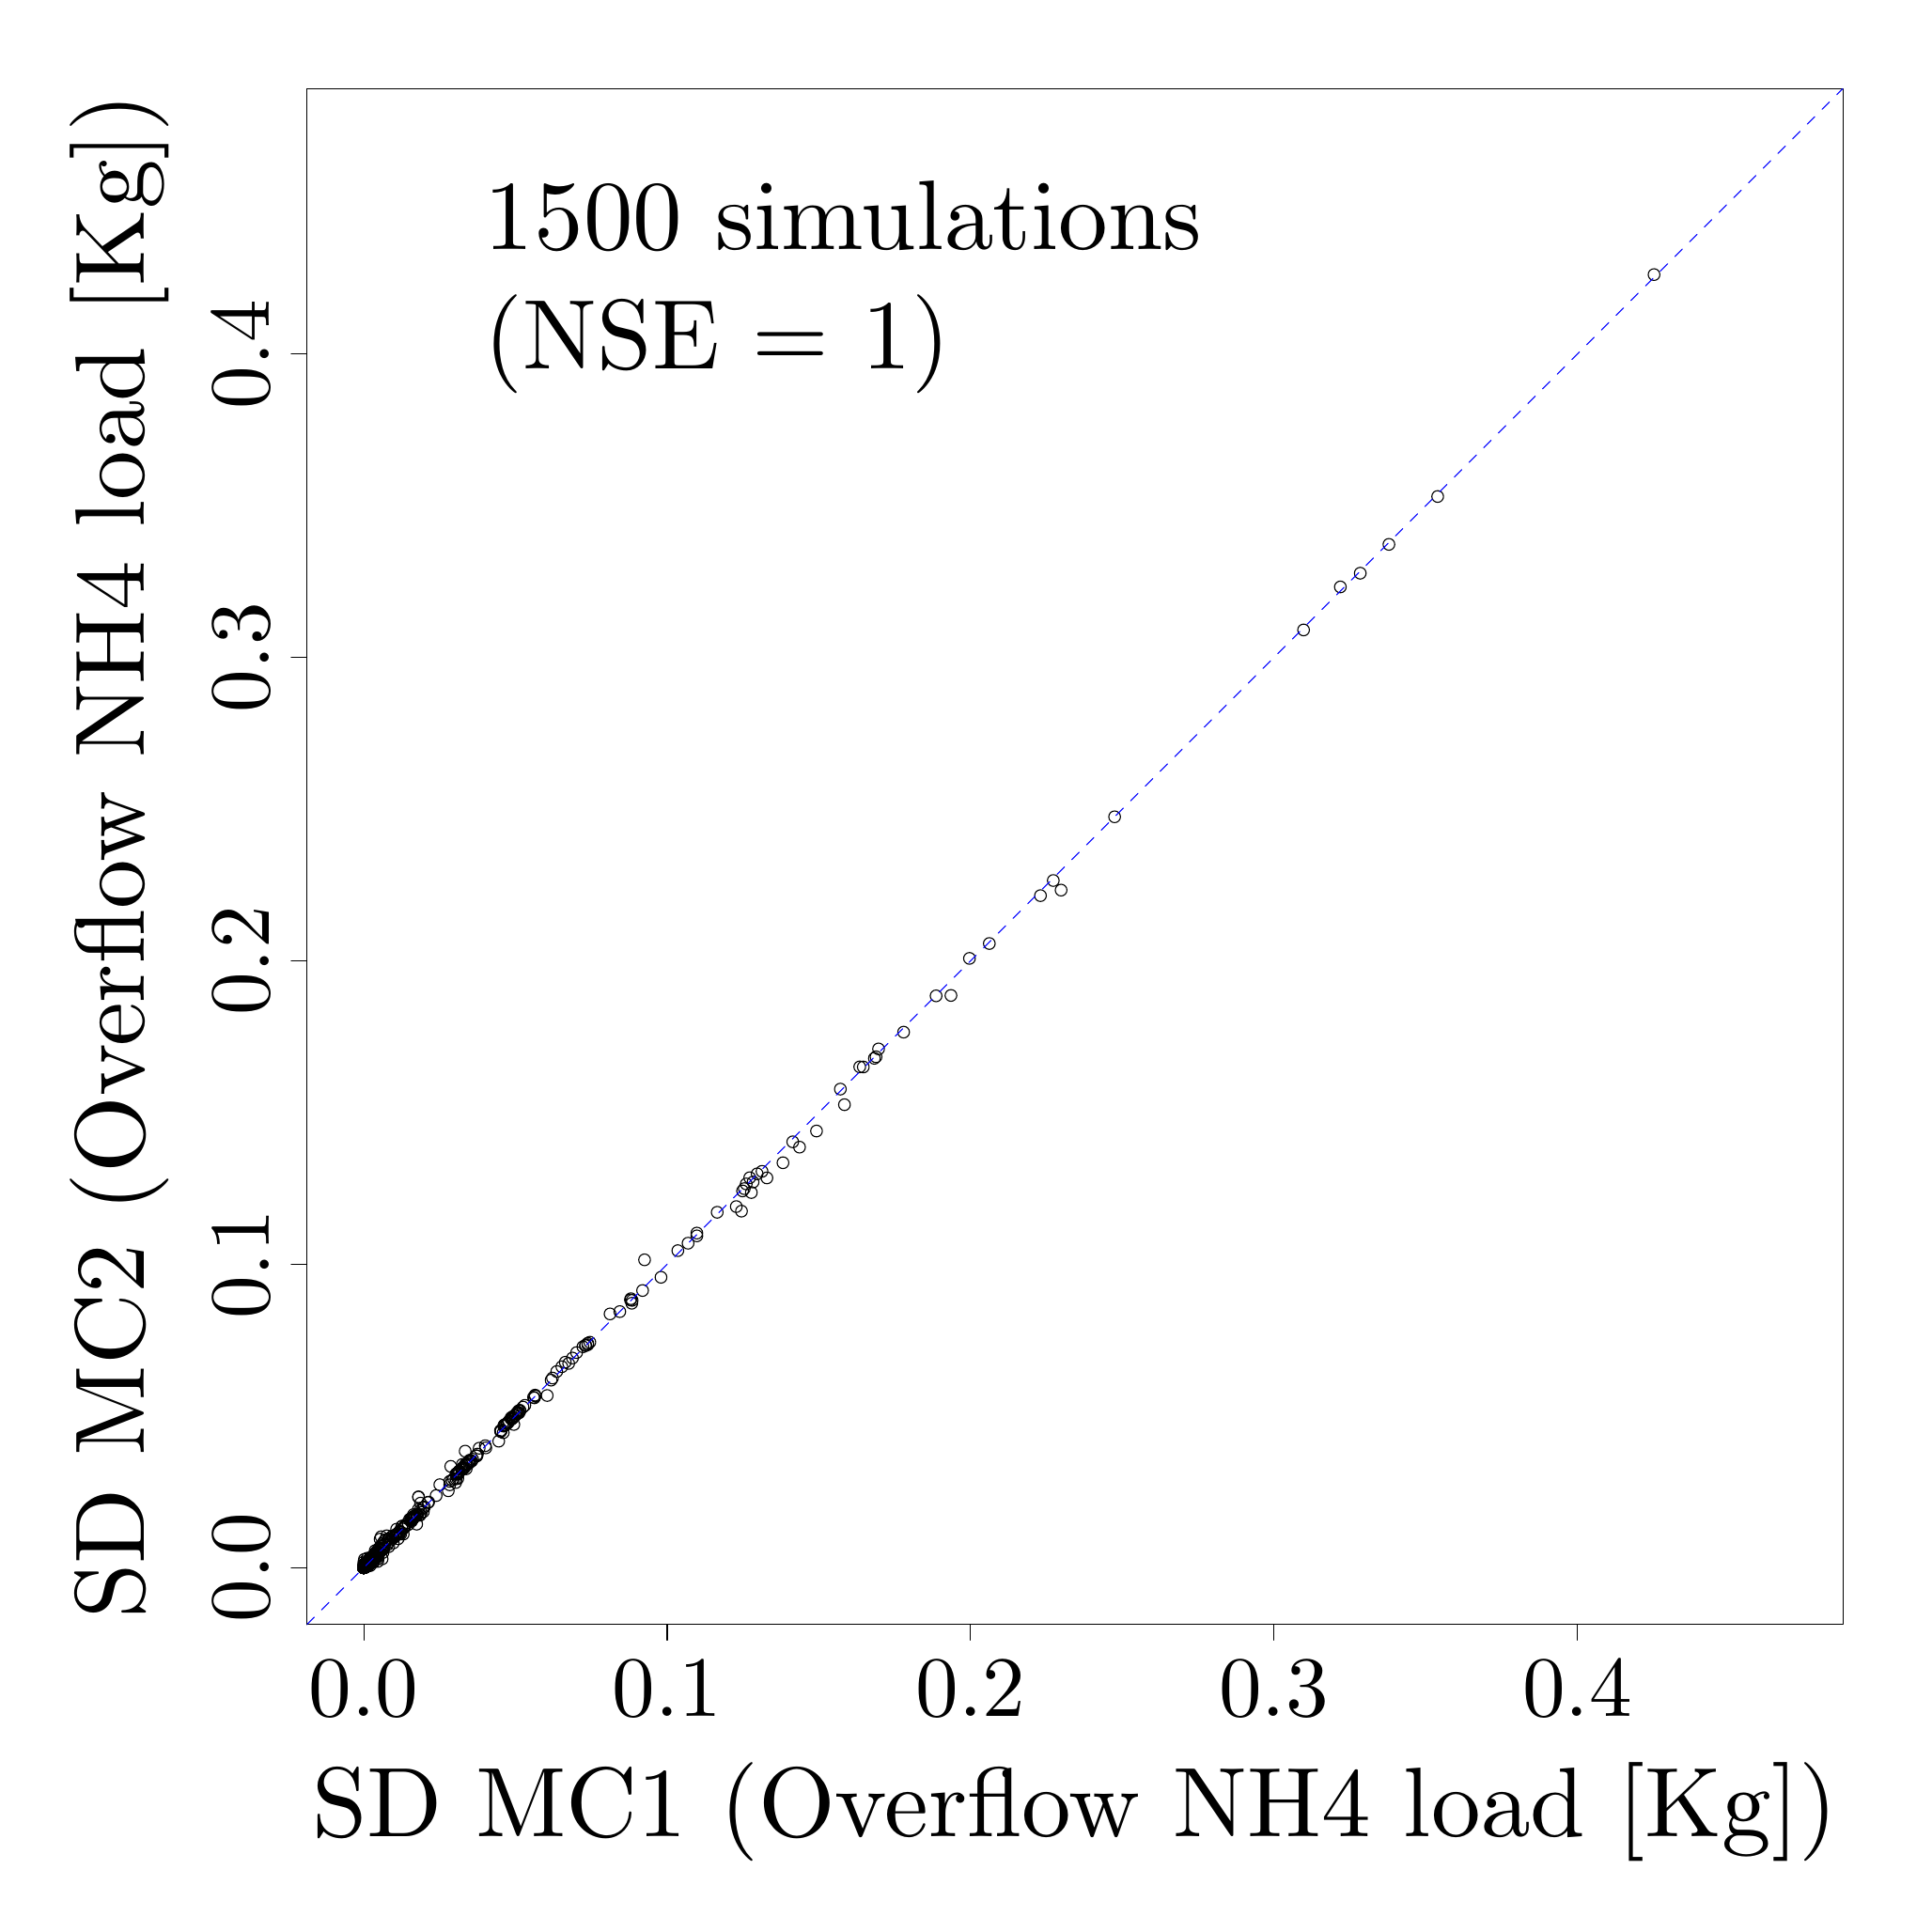
\begin{tikzpicture}[x=1pt,y=1pt]
\definecolor{fillColor}{RGB}{255,255,255}
\path[use as bounding box,fill=fillColor,fill opacity=0.00] (0,0) rectangle (722.70,722.70);
\begin{scope}
\path[clip] (108.00,108.00) rectangle (698.70,698.70);
\definecolor{drawColor}{RGB}{0,0,0}

\path[draw=drawColor,line width= 0.4pt,line join=round,line cap=round] (129.88,129.88) circle (  2.25);

\path[draw=drawColor,line width= 0.4pt,line join=round,line cap=round] (129.88,129.88) circle (  2.25);

\path[draw=drawColor,line width= 0.4pt,line join=round,line cap=round] (129.88,129.88) circle (  2.25);

\path[draw=drawColor,line width= 0.4pt,line join=round,line cap=round] (129.88,129.88) circle (  2.25);

\path[draw=drawColor,line width= 0.4pt,line join=round,line cap=round] (129.88,129.88) circle (  2.25);

\path[draw=drawColor,line width= 0.4pt,line join=round,line cap=round] (129.88,129.88) circle (  2.25);

\path[draw=drawColor,line width= 0.4pt,line join=round,line cap=round] (129.88,129.88) circle (  2.25);

\path[draw=drawColor,line width= 0.4pt,line join=round,line cap=round] (129.88,129.88) circle (  2.25);

\path[draw=drawColor,line width= 0.4pt,line join=round,line cap=round] (129.88,129.88) circle (  2.25);

\path[draw=drawColor,line width= 0.4pt,line join=round,line cap=round] (129.88,129.88) circle (  2.25);

\path[draw=drawColor,line width= 0.4pt,line join=round,line cap=round] (129.88,129.88) circle (  2.25);

\path[draw=drawColor,line width= 0.4pt,line join=round,line cap=round] (129.88,129.88) circle (  2.25);

\path[draw=drawColor,line width= 0.4pt,line join=round,line cap=round] (129.88,129.88) circle (  2.25);

\path[draw=drawColor,line width= 0.4pt,line join=round,line cap=round] (129.88,129.88) circle (  2.25);

\path[draw=drawColor,line width= 0.4pt,line join=round,line cap=round] (129.88,129.88) circle (  2.25);

\path[draw=drawColor,line width= 0.4pt,line join=round,line cap=round] (129.88,129.88) circle (  2.25);

\path[draw=drawColor,line width= 0.4pt,line join=round,line cap=round] (129.88,129.88) circle (  2.25);

\path[draw=drawColor,line width= 0.4pt,line join=round,line cap=round] (129.88,129.88) circle (  2.25);

\path[draw=drawColor,line width= 0.4pt,line join=round,line cap=round] (129.88,129.88) circle (  2.25);

\path[draw=drawColor,line width= 0.4pt,line join=round,line cap=round] (129.88,129.88) circle (  2.25);

\path[draw=drawColor,line width= 0.4pt,line join=round,line cap=round] (129.88,129.88) circle (  2.25);

\path[draw=drawColor,line width= 0.4pt,line join=round,line cap=round] (129.88,129.88) circle (  2.25);

\path[draw=drawColor,line width= 0.4pt,line join=round,line cap=round] (129.88,129.88) circle (  2.25);

\path[draw=drawColor,line width= 0.4pt,line join=round,line cap=round] (129.88,129.88) circle (  2.25);

\path[draw=drawColor,line width= 0.4pt,line join=round,line cap=round] (129.88,129.88) circle (  2.25);

\path[draw=drawColor,line width= 0.4pt,line join=round,line cap=round] (129.88,129.88) circle (  2.25);

\path[draw=drawColor,line width= 0.4pt,line join=round,line cap=round] (129.88,129.88) circle (  2.25);

\path[draw=drawColor,line width= 0.4pt,line join=round,line cap=round] (129.88,129.88) circle (  2.25);

\path[draw=drawColor,line width= 0.4pt,line join=round,line cap=round] (129.88,129.88) circle (  2.25);

\path[draw=drawColor,line width= 0.4pt,line join=round,line cap=round] (129.88,129.88) circle (  2.25);

\path[draw=drawColor,line width= 0.4pt,line join=round,line cap=round] (129.88,129.88) circle (  2.25);

\path[draw=drawColor,line width= 0.4pt,line join=round,line cap=round] (129.88,129.88) circle (  2.25);

\path[draw=drawColor,line width= 0.4pt,line join=round,line cap=round] (129.88,129.88) circle (  2.25);

\path[draw=drawColor,line width= 0.4pt,line join=round,line cap=round] (129.88,129.88) circle (  2.25);

\path[draw=drawColor,line width= 0.4pt,line join=round,line cap=round] (129.88,129.88) circle (  2.25);

\path[draw=drawColor,line width= 0.4pt,line join=round,line cap=round] (129.88,129.88) circle (  2.25);

\path[draw=drawColor,line width= 0.4pt,line join=round,line cap=round] (129.88,129.88) circle (  2.25);

\path[draw=drawColor,line width= 0.4pt,line join=round,line cap=round] (129.88,129.88) circle (  2.25);

\path[draw=drawColor,line width= 0.4pt,line join=round,line cap=round] (129.88,129.88) circle (  2.25);

\path[draw=drawColor,line width= 0.4pt,line join=round,line cap=round] (129.88,129.88) circle (  2.25);

\path[draw=drawColor,line width= 0.4pt,line join=round,line cap=round] (129.88,129.88) circle (  2.25);

\path[draw=drawColor,line width= 0.4pt,line join=round,line cap=round] (129.88,129.88) circle (  2.25);

\path[draw=drawColor,line width= 0.4pt,line join=round,line cap=round] (129.88,129.88) circle (  2.25);

\path[draw=drawColor,line width= 0.4pt,line join=round,line cap=round] (129.88,129.88) circle (  2.25);

\path[draw=drawColor,line width= 0.4pt,line join=round,line cap=round] (129.88,129.88) circle (  2.25);

\path[draw=drawColor,line width= 0.4pt,line join=round,line cap=round] (129.88,129.88) circle (  2.25);

\path[draw=drawColor,line width= 0.4pt,line join=round,line cap=round] (129.88,129.88) circle (  2.25);

\path[draw=drawColor,line width= 0.4pt,line join=round,line cap=round] (129.88,129.88) circle (  2.25);

\path[draw=drawColor,line width= 0.4pt,line join=round,line cap=round] (129.88,129.88) circle (  2.25);

\path[draw=drawColor,line width= 0.4pt,line join=round,line cap=round] (129.88,129.88) circle (  2.25);

\path[draw=drawColor,line width= 0.4pt,line join=round,line cap=round] (129.88,129.88) circle (  2.25);

\path[draw=drawColor,line width= 0.4pt,line join=round,line cap=round] (129.88,129.88) circle (  2.25);

\path[draw=drawColor,line width= 0.4pt,line join=round,line cap=round] (129.88,129.88) circle (  2.25);

\path[draw=drawColor,line width= 0.4pt,line join=round,line cap=round] (129.88,129.88) circle (  2.25);

\path[draw=drawColor,line width= 0.4pt,line join=round,line cap=round] (129.88,129.88) circle (  2.25);

\path[draw=drawColor,line width= 0.4pt,line join=round,line cap=round] (129.88,129.88) circle (  2.25);

\path[draw=drawColor,line width= 0.4pt,line join=round,line cap=round] (129.88,129.88) circle (  2.25);

\path[draw=drawColor,line width= 0.4pt,line join=round,line cap=round] (129.88,129.88) circle (  2.25);

\path[draw=drawColor,line width= 0.4pt,line join=round,line cap=round] (129.88,129.88) circle (  2.25);

\path[draw=drawColor,line width= 0.4pt,line join=round,line cap=round] (129.88,129.88) circle (  2.25);

\path[draw=drawColor,line width= 0.4pt,line join=round,line cap=round] (129.88,129.88) circle (  2.25);

\path[draw=drawColor,line width= 0.4pt,line join=round,line cap=round] (129.88,129.88) circle (  2.25);

\path[draw=drawColor,line width= 0.4pt,line join=round,line cap=round] (129.88,129.88) circle (  2.25);

\path[draw=drawColor,line width= 0.4pt,line join=round,line cap=round] (129.88,129.88) circle (  2.25);

\path[draw=drawColor,line width= 0.4pt,line join=round,line cap=round] (129.88,129.88) circle (  2.25);

\path[draw=drawColor,line width= 0.4pt,line join=round,line cap=round] (129.88,129.88) circle (  2.25);

\path[draw=drawColor,line width= 0.4pt,line join=round,line cap=round] (129.88,129.88) circle (  2.25);

\path[draw=drawColor,line width= 0.4pt,line join=round,line cap=round] (129.88,129.88) circle (  2.25);

\path[draw=drawColor,line width= 0.4pt,line join=round,line cap=round] (129.88,129.88) circle (  2.25);

\path[draw=drawColor,line width= 0.4pt,line join=round,line cap=round] (129.88,129.88) circle (  2.25);

\path[draw=drawColor,line width= 0.4pt,line join=round,line cap=round] (129.88,129.88) circle (  2.25);

\path[draw=drawColor,line width= 0.4pt,line join=round,line cap=round] (129.88,129.88) circle (  2.25);

\path[draw=drawColor,line width= 0.4pt,line join=round,line cap=round] (129.88,129.88) circle (  2.25);

\path[draw=drawColor,line width= 0.4pt,line join=round,line cap=round] (129.88,129.88) circle (  2.25);

\path[draw=drawColor,line width= 0.4pt,line join=round,line cap=round] (129.88,129.88) circle (  2.25);

\path[draw=drawColor,line width= 0.4pt,line join=round,line cap=round] (129.88,129.88) circle (  2.25);

\path[draw=drawColor,line width= 0.4pt,line join=round,line cap=round] (129.88,129.88) circle (  2.25);

\path[draw=drawColor,line width= 0.4pt,line join=round,line cap=round] (129.88,129.88) circle (  2.25);

\path[draw=drawColor,line width= 0.4pt,line join=round,line cap=round] (129.88,129.88) circle (  2.25);

\path[draw=drawColor,line width= 0.4pt,line join=round,line cap=round] (129.88,129.88) circle (  2.25);

\path[draw=drawColor,line width= 0.4pt,line join=round,line cap=round] (129.88,129.88) circle (  2.25);

\path[draw=drawColor,line width= 0.4pt,line join=round,line cap=round] (129.88,129.88) circle (  2.25);

\path[draw=drawColor,line width= 0.4pt,line join=round,line cap=round] (129.88,129.88) circle (  2.25);

\path[draw=drawColor,line width= 0.4pt,line join=round,line cap=round] (129.88,129.88) circle (  2.25);

\path[draw=drawColor,line width= 0.4pt,line join=round,line cap=round] (129.88,129.88) circle (  2.25);

\path[draw=drawColor,line width= 0.4pt,line join=round,line cap=round] (129.88,129.88) circle (  2.25);

\path[draw=drawColor,line width= 0.4pt,line join=round,line cap=round] (129.88,129.88) circle (  2.25);

\path[draw=drawColor,line width= 0.4pt,line join=round,line cap=round] (129.88,129.88) circle (  2.25);

\path[draw=drawColor,line width= 0.4pt,line join=round,line cap=round] (129.88,129.88) circle (  2.25);

\path[draw=drawColor,line width= 0.4pt,line join=round,line cap=round] (129.88,129.88) circle (  2.25);

\path[draw=drawColor,line width= 0.4pt,line join=round,line cap=round] (129.88,129.88) circle (  2.25);

\path[draw=drawColor,line width= 0.4pt,line join=round,line cap=round] (129.88,129.88) circle (  2.25);

\path[draw=drawColor,line width= 0.4pt,line join=round,line cap=round] (129.88,129.88) circle (  2.25);

\path[draw=drawColor,line width= 0.4pt,line join=round,line cap=round] (129.88,129.88) circle (  2.25);

\path[draw=drawColor,line width= 0.4pt,line join=round,line cap=round] (129.88,129.88) circle (  2.25);

\path[draw=drawColor,line width= 0.4pt,line join=round,line cap=round] (129.88,129.88) circle (  2.25);

\path[draw=drawColor,line width= 0.4pt,line join=round,line cap=round] (129.88,129.88) circle (  2.25);

\path[draw=drawColor,line width= 0.4pt,line join=round,line cap=round] (129.88,129.88) circle (  2.25);

\path[draw=drawColor,line width= 0.4pt,line join=round,line cap=round] (129.88,129.88) circle (  2.25);

\path[draw=drawColor,line width= 0.4pt,line join=round,line cap=round] (129.88,129.88) circle (  2.25);

\path[draw=drawColor,line width= 0.4pt,line join=round,line cap=round] (129.88,129.88) circle (  2.25);

\path[draw=drawColor,line width= 0.4pt,line join=round,line cap=round] (129.88,129.88) circle (  2.25);

\path[draw=drawColor,line width= 0.4pt,line join=round,line cap=round] (129.88,129.88) circle (  2.25);

\path[draw=drawColor,line width= 0.4pt,line join=round,line cap=round] (129.88,129.88) circle (  2.25);

\path[draw=drawColor,line width= 0.4pt,line join=round,line cap=round] (129.88,129.88) circle (  2.25);

\path[draw=drawColor,line width= 0.4pt,line join=round,line cap=round] (129.88,129.88) circle (  2.25);

\path[draw=drawColor,line width= 0.4pt,line join=round,line cap=round] (129.88,129.88) circle (  2.25);

\path[draw=drawColor,line width= 0.4pt,line join=round,line cap=round] (129.88,129.88) circle (  2.25);

\path[draw=drawColor,line width= 0.4pt,line join=round,line cap=round] (129.88,129.88) circle (  2.25);

\path[draw=drawColor,line width= 0.4pt,line join=round,line cap=round] (129.88,129.88) circle (  2.25);

\path[draw=drawColor,line width= 0.4pt,line join=round,line cap=round] (129.88,129.88) circle (  2.25);

\path[draw=drawColor,line width= 0.4pt,line join=round,line cap=round] (129.88,129.88) circle (  2.25);

\path[draw=drawColor,line width= 0.4pt,line join=round,line cap=round] (129.88,129.88) circle (  2.25);

\path[draw=drawColor,line width= 0.4pt,line join=round,line cap=round] (129.88,129.88) circle (  2.25);

\path[draw=drawColor,line width= 0.4pt,line join=round,line cap=round] (129.88,129.88) circle (  2.25);

\path[draw=drawColor,line width= 0.4pt,line join=round,line cap=round] (129.88,129.88) circle (  2.25);

\path[draw=drawColor,line width= 0.4pt,line join=round,line cap=round] (129.88,129.88) circle (  2.25);

\path[draw=drawColor,line width= 0.4pt,line join=round,line cap=round] (129.88,129.88) circle (  2.25);

\path[draw=drawColor,line width= 0.4pt,line join=round,line cap=round] (129.88,129.88) circle (  2.25);

\path[draw=drawColor,line width= 0.4pt,line join=round,line cap=round] (129.88,129.88) circle (  2.25);

\path[draw=drawColor,line width= 0.4pt,line join=round,line cap=round] (129.88,129.88) circle (  2.25);

\path[draw=drawColor,line width= 0.4pt,line join=round,line cap=round] (129.88,129.88) circle (  2.25);

\path[draw=drawColor,line width= 0.4pt,line join=round,line cap=round] (129.88,129.88) circle (  2.25);

\path[draw=drawColor,line width= 0.4pt,line join=round,line cap=round] (129.88,129.88) circle (  2.25);

\path[draw=drawColor,line width= 0.4pt,line join=round,line cap=round] (129.88,129.88) circle (  2.25);

\path[draw=drawColor,line width= 0.4pt,line join=round,line cap=round] (129.88,129.88) circle (  2.25);

\path[draw=drawColor,line width= 0.4pt,line join=round,line cap=round] (129.88,129.88) circle (  2.25);

\path[draw=drawColor,line width= 0.4pt,line join=round,line cap=round] (129.88,129.88) circle (  2.25);

\path[draw=drawColor,line width= 0.4pt,line join=round,line cap=round] (129.88,129.88) circle (  2.25);

\path[draw=drawColor,line width= 0.4pt,line join=round,line cap=round] (129.88,129.88) circle (  2.25);

\path[draw=drawColor,line width= 0.4pt,line join=round,line cap=round] (129.88,129.88) circle (  2.25);

\path[draw=drawColor,line width= 0.4pt,line join=round,line cap=round] (129.88,129.88) circle (  2.25);

\path[draw=drawColor,line width= 0.4pt,line join=round,line cap=round] (129.88,129.88) circle (  2.25);

\path[draw=drawColor,line width= 0.4pt,line join=round,line cap=round] (129.88,129.88) circle (  2.25);

\path[draw=drawColor,line width= 0.4pt,line join=round,line cap=round] (129.88,129.88) circle (  2.25);

\path[draw=drawColor,line width= 0.4pt,line join=round,line cap=round] (129.88,129.88) circle (  2.25);

\path[draw=drawColor,line width= 0.4pt,line join=round,line cap=round] (129.88,129.88) circle (  2.25);

\path[draw=drawColor,line width= 0.4pt,line join=round,line cap=round] (129.88,129.88) circle (  2.25);

\path[draw=drawColor,line width= 0.4pt,line join=round,line cap=round] (129.88,129.88) circle (  2.25);

\path[draw=drawColor,line width= 0.4pt,line join=round,line cap=round] (129.88,129.88) circle (  2.25);

\path[draw=drawColor,line width= 0.4pt,line join=round,line cap=round] (129.88,129.88) circle (  2.25);

\path[draw=drawColor,line width= 0.4pt,line join=round,line cap=round] (129.88,129.88) circle (  2.25);

\path[draw=drawColor,line width= 0.4pt,line join=round,line cap=round] (129.88,129.88) circle (  2.25);

\path[draw=drawColor,line width= 0.4pt,line join=round,line cap=round] (129.88,129.88) circle (  2.25);

\path[draw=drawColor,line width= 0.4pt,line join=round,line cap=round] (129.88,129.88) circle (  2.25);

\path[draw=drawColor,line width= 0.4pt,line join=round,line cap=round] (129.88,129.88) circle (  2.25);

\path[draw=drawColor,line width= 0.4pt,line join=round,line cap=round] (129.88,129.88) circle (  2.25);

\path[draw=drawColor,line width= 0.4pt,line join=round,line cap=round] (129.88,129.88) circle (  2.25);

\path[draw=drawColor,line width= 0.4pt,line join=round,line cap=round] (129.88,129.88) circle (  2.25);

\path[draw=drawColor,line width= 0.4pt,line join=round,line cap=round] (129.88,129.88) circle (  2.25);

\path[draw=drawColor,line width= 0.4pt,line join=round,line cap=round] (129.88,129.88) circle (  2.25);

\path[draw=drawColor,line width= 0.4pt,line join=round,line cap=round] (129.88,129.88) circle (  2.25);

\path[draw=drawColor,line width= 0.4pt,line join=round,line cap=round] (129.88,129.88) circle (  2.25);

\path[draw=drawColor,line width= 0.4pt,line join=round,line cap=round] (129.88,129.88) circle (  2.25);

\path[draw=drawColor,line width= 0.4pt,line join=round,line cap=round] (129.88,129.88) circle (  2.25);

\path[draw=drawColor,line width= 0.4pt,line join=round,line cap=round] (129.88,129.88) circle (  2.25);

\path[draw=drawColor,line width= 0.4pt,line join=round,line cap=round] (129.88,129.88) circle (  2.25);

\path[draw=drawColor,line width= 0.4pt,line join=round,line cap=round] (129.88,129.88) circle (  2.25);

\path[draw=drawColor,line width= 0.4pt,line join=round,line cap=round] (129.88,129.88) circle (  2.25);

\path[draw=drawColor,line width= 0.4pt,line join=round,line cap=round] (129.88,129.88) circle (  2.25);

\path[draw=drawColor,line width= 0.4pt,line join=round,line cap=round] (129.88,129.88) circle (  2.25);

\path[draw=drawColor,line width= 0.4pt,line join=round,line cap=round] (129.88,129.88) circle (  2.25);

\path[draw=drawColor,line width= 0.4pt,line join=round,line cap=round] (129.88,129.88) circle (  2.25);

\path[draw=drawColor,line width= 0.4pt,line join=round,line cap=round] (129.88,129.88) circle (  2.25);

\path[draw=drawColor,line width= 0.4pt,line join=round,line cap=round] (129.88,129.88) circle (  2.25);

\path[draw=drawColor,line width= 0.4pt,line join=round,line cap=round] (129.88,129.88) circle (  2.25);

\path[draw=drawColor,line width= 0.4pt,line join=round,line cap=round] (129.88,129.88) circle (  2.25);

\path[draw=drawColor,line width= 0.4pt,line join=round,line cap=round] (129.88,129.88) circle (  2.25);

\path[draw=drawColor,line width= 0.4pt,line join=round,line cap=round] (129.88,129.88) circle (  2.25);

\path[draw=drawColor,line width= 0.4pt,line join=round,line cap=round] (129.88,129.88) circle (  2.25);

\path[draw=drawColor,line width= 0.4pt,line join=round,line cap=round] (129.88,129.88) circle (  2.25);

\path[draw=drawColor,line width= 0.4pt,line join=round,line cap=round] (129.88,129.88) circle (  2.25);

\path[draw=drawColor,line width= 0.4pt,line join=round,line cap=round] (129.88,129.88) circle (  2.25);

\path[draw=drawColor,line width= 0.4pt,line join=round,line cap=round] (129.88,129.88) circle (  2.25);

\path[draw=drawColor,line width= 0.4pt,line join=round,line cap=round] (129.88,129.88) circle (  2.25);

\path[draw=drawColor,line width= 0.4pt,line join=round,line cap=round] (129.88,129.88) circle (  2.25);

\path[draw=drawColor,line width= 0.4pt,line join=round,line cap=round] (129.88,129.88) circle (  2.25);

\path[draw=drawColor,line width= 0.4pt,line join=round,line cap=round] (129.88,129.88) circle (  2.25);

\path[draw=drawColor,line width= 0.4pt,line join=round,line cap=round] (129.88,129.88) circle (  2.25);

\path[draw=drawColor,line width= 0.4pt,line join=round,line cap=round] (129.88,129.88) circle (  2.25);

\path[draw=drawColor,line width= 0.4pt,line join=round,line cap=round] (129.88,129.88) circle (  2.25);

\path[draw=drawColor,line width= 0.4pt,line join=round,line cap=round] (129.88,129.88) circle (  2.25);

\path[draw=drawColor,line width= 0.4pt,line join=round,line cap=round] (129.88,129.88) circle (  2.25);

\path[draw=drawColor,line width= 0.4pt,line join=round,line cap=round] (129.88,129.88) circle (  2.25);

\path[draw=drawColor,line width= 0.4pt,line join=round,line cap=round] (129.88,129.88) circle (  2.25);

\path[draw=drawColor,line width= 0.4pt,line join=round,line cap=round] (129.88,129.88) circle (  2.25);

\path[draw=drawColor,line width= 0.4pt,line join=round,line cap=round] (129.88,129.88) circle (  2.25);

\path[draw=drawColor,line width= 0.4pt,line join=round,line cap=round] (129.88,129.88) circle (  2.25);

\path[draw=drawColor,line width= 0.4pt,line join=round,line cap=round] (129.88,129.88) circle (  2.25);

\path[draw=drawColor,line width= 0.4pt,line join=round,line cap=round] (129.88,129.88) circle (  2.25);

\path[draw=drawColor,line width= 0.4pt,line join=round,line cap=round] (129.88,129.88) circle (  2.25);

\path[draw=drawColor,line width= 0.4pt,line join=round,line cap=round] (129.88,129.88) circle (  2.25);

\path[draw=drawColor,line width= 0.4pt,line join=round,line cap=round] (129.88,129.88) circle (  2.25);

\path[draw=drawColor,line width= 0.4pt,line join=round,line cap=round] (129.88,129.88) circle (  2.25);

\path[draw=drawColor,line width= 0.4pt,line join=round,line cap=round] (129.88,129.88) circle (  2.25);

\path[draw=drawColor,line width= 0.4pt,line join=round,line cap=round] (129.88,129.88) circle (  2.25);

\path[draw=drawColor,line width= 0.4pt,line join=round,line cap=round] (129.88,129.88) circle (  2.25);

\path[draw=drawColor,line width= 0.4pt,line join=round,line cap=round] (129.88,129.88) circle (  2.25);

\path[draw=drawColor,line width= 0.4pt,line join=round,line cap=round] (129.88,129.88) circle (  2.25);

\path[draw=drawColor,line width= 0.4pt,line join=round,line cap=round] (129.88,129.88) circle (  2.25);

\path[draw=drawColor,line width= 0.4pt,line join=round,line cap=round] (129.88,129.88) circle (  2.25);

\path[draw=drawColor,line width= 0.4pt,line join=round,line cap=round] (129.88,129.88) circle (  2.25);

\path[draw=drawColor,line width= 0.4pt,line join=round,line cap=round] (129.88,129.88) circle (  2.25);

\path[draw=drawColor,line width= 0.4pt,line join=round,line cap=round] (129.88,129.88) circle (  2.25);

\path[draw=drawColor,line width= 0.4pt,line join=round,line cap=round] (129.88,129.88) circle (  2.25);

\path[draw=drawColor,line width= 0.4pt,line join=round,line cap=round] (129.88,129.88) circle (  2.25);

\path[draw=drawColor,line width= 0.4pt,line join=round,line cap=round] (129.88,129.88) circle (  2.25);

\path[draw=drawColor,line width= 0.4pt,line join=round,line cap=round] (129.88,129.88) circle (  2.25);

\path[draw=drawColor,line width= 0.4pt,line join=round,line cap=round] (129.88,129.88) circle (  2.25);

\path[draw=drawColor,line width= 0.4pt,line join=round,line cap=round] (129.88,129.88) circle (  2.25);

\path[draw=drawColor,line width= 0.4pt,line join=round,line cap=round] (129.88,129.88) circle (  2.25);

\path[draw=drawColor,line width= 0.4pt,line join=round,line cap=round] (129.88,129.88) circle (  2.25);

\path[draw=drawColor,line width= 0.4pt,line join=round,line cap=round] (129.88,129.88) circle (  2.25);

\path[draw=drawColor,line width= 0.4pt,line join=round,line cap=round] (129.88,129.88) circle (  2.25);

\path[draw=drawColor,line width= 0.4pt,line join=round,line cap=round] (129.88,129.88) circle (  2.25);

\path[draw=drawColor,line width= 0.4pt,line join=round,line cap=round] (129.88,129.88) circle (  2.25);

\path[draw=drawColor,line width= 0.4pt,line join=round,line cap=round] (129.88,129.88) circle (  2.25);

\path[draw=drawColor,line width= 0.4pt,line join=round,line cap=round] (129.88,129.88) circle (  2.25);

\path[draw=drawColor,line width= 0.4pt,line join=round,line cap=round] (129.88,129.88) circle (  2.25);

\path[draw=drawColor,line width= 0.4pt,line join=round,line cap=round] (129.88,129.88) circle (  2.25);

\path[draw=drawColor,line width= 0.4pt,line join=round,line cap=round] (129.88,129.88) circle (  2.25);

\path[draw=drawColor,line width= 0.4pt,line join=round,line cap=round] (129.88,129.88) circle (  2.25);

\path[draw=drawColor,line width= 0.4pt,line join=round,line cap=round] (129.88,129.88) circle (  2.25);

\path[draw=drawColor,line width= 0.4pt,line join=round,line cap=round] (129.88,129.88) circle (  2.25);

\path[draw=drawColor,line width= 0.4pt,line join=round,line cap=round] (129.88,129.88) circle (  2.25);

\path[draw=drawColor,line width= 0.4pt,line join=round,line cap=round] (129.88,129.88) circle (  2.25);

\path[draw=drawColor,line width= 0.4pt,line join=round,line cap=round] (129.88,129.88) circle (  2.25);

\path[draw=drawColor,line width= 0.4pt,line join=round,line cap=round] (129.88,129.88) circle (  2.25);

\path[draw=drawColor,line width= 0.4pt,line join=round,line cap=round] (129.88,129.88) circle (  2.25);

\path[draw=drawColor,line width= 0.4pt,line join=round,line cap=round] (129.88,129.88) circle (  2.25);

\path[draw=drawColor,line width= 0.4pt,line join=round,line cap=round] (129.88,129.88) circle (  2.25);

\path[draw=drawColor,line width= 0.4pt,line join=round,line cap=round] (129.88,129.88) circle (  2.25);

\path[draw=drawColor,line width= 0.4pt,line join=round,line cap=round] (129.88,129.88) circle (  2.25);

\path[draw=drawColor,line width= 0.4pt,line join=round,line cap=round] (129.88,129.88) circle (  2.25);

\path[draw=drawColor,line width= 0.4pt,line join=round,line cap=round] (129.88,129.88) circle (  2.25);

\path[draw=drawColor,line width= 0.4pt,line join=round,line cap=round] (129.88,129.88) circle (  2.25);

\path[draw=drawColor,line width= 0.4pt,line join=round,line cap=round] (129.88,129.88) circle (  2.25);

\path[draw=drawColor,line width= 0.4pt,line join=round,line cap=round] (129.88,129.88) circle (  2.25);

\path[draw=drawColor,line width= 0.4pt,line join=round,line cap=round] (129.88,129.88) circle (  2.25);

\path[draw=drawColor,line width= 0.4pt,line join=round,line cap=round] (129.88,129.88) circle (  2.25);

\path[draw=drawColor,line width= 0.4pt,line join=round,line cap=round] (129.88,129.88) circle (  2.25);

\path[draw=drawColor,line width= 0.4pt,line join=round,line cap=round] (129.88,129.88) circle (  2.25);

\path[draw=drawColor,line width= 0.4pt,line join=round,line cap=round] (129.88,129.88) circle (  2.25);

\path[draw=drawColor,line width= 0.4pt,line join=round,line cap=round] (129.88,129.88) circle (  2.25);

\path[draw=drawColor,line width= 0.4pt,line join=round,line cap=round] (129.88,129.88) circle (  2.25);

\path[draw=drawColor,line width= 0.4pt,line join=round,line cap=round] (129.88,129.88) circle (  2.25);

\path[draw=drawColor,line width= 0.4pt,line join=round,line cap=round] (129.88,129.88) circle (  2.25);

\path[draw=drawColor,line width= 0.4pt,line join=round,line cap=round] (129.88,129.88) circle (  2.25);

\path[draw=drawColor,line width= 0.4pt,line join=round,line cap=round] (129.88,129.88) circle (  2.25);

\path[draw=drawColor,line width= 0.4pt,line join=round,line cap=round] (129.88,129.88) circle (  2.25);

\path[draw=drawColor,line width= 0.4pt,line join=round,line cap=round] (129.88,129.88) circle (  2.25);

\path[draw=drawColor,line width= 0.4pt,line join=round,line cap=round] (129.88,129.88) circle (  2.25);

\path[draw=drawColor,line width= 0.4pt,line join=round,line cap=round] (129.88,129.88) circle (  2.25);

\path[draw=drawColor,line width= 0.4pt,line join=round,line cap=round] (129.88,129.88) circle (  2.25);

\path[draw=drawColor,line width= 0.4pt,line join=round,line cap=round] (129.88,129.88) circle (  2.25);

\path[draw=drawColor,line width= 0.4pt,line join=round,line cap=round] (129.88,129.88) circle (  2.25);

\path[draw=drawColor,line width= 0.4pt,line join=round,line cap=round] (129.88,129.88) circle (  2.25);

\path[draw=drawColor,line width= 0.4pt,line join=round,line cap=round] (129.88,129.88) circle (  2.25);

\path[draw=drawColor,line width= 0.4pt,line join=round,line cap=round] (129.88,129.88) circle (  2.25);

\path[draw=drawColor,line width= 0.4pt,line join=round,line cap=round] (129.88,129.88) circle (  2.25);

\path[draw=drawColor,line width= 0.4pt,line join=round,line cap=round] (129.88,129.88) circle (  2.25);

\path[draw=drawColor,line width= 0.4pt,line join=round,line cap=round] (129.88,129.88) circle (  2.25);

\path[draw=drawColor,line width= 0.4pt,line join=round,line cap=round] (129.88,129.88) circle (  2.25);

\path[draw=drawColor,line width= 0.4pt,line join=round,line cap=round] (129.88,129.88) circle (  2.25);

\path[draw=drawColor,line width= 0.4pt,line join=round,line cap=round] (129.88,129.88) circle (  2.25);

\path[draw=drawColor,line width= 0.4pt,line join=round,line cap=round] (129.88,129.88) circle (  2.25);

\path[draw=drawColor,line width= 0.4pt,line join=round,line cap=round] (129.88,129.88) circle (  2.25);

\path[draw=drawColor,line width= 0.4pt,line join=round,line cap=round] (129.88,129.88) circle (  2.25);

\path[draw=drawColor,line width= 0.4pt,line join=round,line cap=round] (129.88,129.88) circle (  2.25);

\path[draw=drawColor,line width= 0.4pt,line join=round,line cap=round] (129.88,129.88) circle (  2.25);

\path[draw=drawColor,line width= 0.4pt,line join=round,line cap=round] (129.88,129.88) circle (  2.25);

\path[draw=drawColor,line width= 0.4pt,line join=round,line cap=round] (129.88,129.88) circle (  2.25);

\path[draw=drawColor,line width= 0.4pt,line join=round,line cap=round] (129.88,129.88) circle (  2.25);

\path[draw=drawColor,line width= 0.4pt,line join=round,line cap=round] (129.88,129.88) circle (  2.25);

\path[draw=drawColor,line width= 0.4pt,line join=round,line cap=round] (129.88,129.88) circle (  2.25);

\path[draw=drawColor,line width= 0.4pt,line join=round,line cap=round] (129.88,129.88) circle (  2.25);

\path[draw=drawColor,line width= 0.4pt,line join=round,line cap=round] (129.88,129.88) circle (  2.25);

\path[draw=drawColor,line width= 0.4pt,line join=round,line cap=round] (131.22,133.49) circle (  2.25);

\path[draw=drawColor,line width= 0.4pt,line join=round,line cap=round] (173.59,173.54) circle (  2.25);

\path[draw=drawColor,line width= 0.4pt,line join=round,line cap=round] (162.38,159.43) circle (  2.25);

\path[draw=drawColor,line width= 0.4pt,line join=round,line cap=round] (166.03,164.15) circle (  2.25);

\path[draw=drawColor,line width= 0.4pt,line join=round,line cap=round] (168.42,168.10) circle (  2.25);

\path[draw=drawColor,line width= 0.4pt,line join=round,line cap=round] (170.55,171.15) circle (  2.25);

\path[draw=drawColor,line width= 0.4pt,line join=round,line cap=round] (149.41,149.58) circle (  2.25);

\path[draw=drawColor,line width= 0.4pt,line join=round,line cap=round] (130.54,130.18) circle (  2.25);

\path[draw=drawColor,line width= 0.4pt,line join=round,line cap=round] (130.30,129.88) circle (  2.25);

\path[draw=drawColor,line width= 0.4pt,line join=round,line cap=round] (130.09,129.88) circle (  2.25);

\path[draw=drawColor,line width= 0.4pt,line join=round,line cap=round] (129.90,129.88) circle (  2.25);

\path[draw=drawColor,line width= 0.4pt,line join=round,line cap=round] (129.88,129.88) circle (  2.25);

\path[draw=drawColor,line width= 0.4pt,line join=round,line cap=round] (129.88,129.88) circle (  2.25);

\path[draw=drawColor,line width= 0.4pt,line join=round,line cap=round] (129.88,129.88) circle (  2.25);

\path[draw=drawColor,line width= 0.4pt,line join=round,line cap=round] (129.88,129.88) circle (  2.25);

\path[draw=drawColor,line width= 0.4pt,line join=round,line cap=round] (129.88,129.88) circle (  2.25);

\path[draw=drawColor,line width= 0.4pt,line join=round,line cap=round] (129.88,129.88) circle (  2.25);

\path[draw=drawColor,line width= 0.4pt,line join=round,line cap=round] (129.88,129.88) circle (  2.25);

\path[draw=drawColor,line width= 0.4pt,line join=round,line cap=round] (129.88,129.88) circle (  2.25);

\path[draw=drawColor,line width= 0.4pt,line join=round,line cap=round] (129.88,129.88) circle (  2.25);

\path[draw=drawColor,line width= 0.4pt,line join=round,line cap=round] (129.88,129.88) circle (  2.25);

\path[draw=drawColor,line width= 0.4pt,line join=round,line cap=round] (129.88,129.88) circle (  2.25);

\path[draw=drawColor,line width= 0.4pt,line join=round,line cap=round] (129.88,129.88) circle (  2.25);

\path[draw=drawColor,line width= 0.4pt,line join=round,line cap=round] (129.88,129.88) circle (  2.25);

\path[draw=drawColor,line width= 0.4pt,line join=round,line cap=round] (129.88,129.88) circle (  2.25);

\path[draw=drawColor,line width= 0.4pt,line join=round,line cap=round] (129.88,129.88) circle (  2.25);

\path[draw=drawColor,line width= 0.4pt,line join=round,line cap=round] (129.88,129.88) circle (  2.25);

\path[draw=drawColor,line width= 0.4pt,line join=round,line cap=round] (129.88,129.88) circle (  2.25);

\path[draw=drawColor,line width= 0.4pt,line join=round,line cap=round] (129.88,129.88) circle (  2.25);

\path[draw=drawColor,line width= 0.4pt,line join=round,line cap=round] (129.88,129.88) circle (  2.25);

\path[draw=drawColor,line width= 0.4pt,line join=round,line cap=round] (129.88,129.88) circle (  2.25);

\path[draw=drawColor,line width= 0.4pt,line join=round,line cap=round] (129.88,129.88) circle (  2.25);

\path[draw=drawColor,line width= 0.4pt,line join=round,line cap=round] (129.88,129.88) circle (  2.25);

\path[draw=drawColor,line width= 0.4pt,line join=round,line cap=round] (129.88,129.88) circle (  2.25);

\path[draw=drawColor,line width= 0.4pt,line join=round,line cap=round] (129.88,129.88) circle (  2.25);

\path[draw=drawColor,line width= 0.4pt,line join=round,line cap=round] (129.88,129.88) circle (  2.25);

\path[draw=drawColor,line width= 0.4pt,line join=round,line cap=round] (129.88,129.88) circle (  2.25);

\path[draw=drawColor,line width= 0.4pt,line join=round,line cap=round] (129.88,129.88) circle (  2.25);

\path[draw=drawColor,line width= 0.4pt,line join=round,line cap=round] (129.88,129.88) circle (  2.25);

\path[draw=drawColor,line width= 0.4pt,line join=round,line cap=round] (129.88,129.88) circle (  2.25);

\path[draw=drawColor,line width= 0.4pt,line join=round,line cap=round] (129.88,129.88) circle (  2.25);

\path[draw=drawColor,line width= 0.4pt,line join=round,line cap=round] (129.88,129.88) circle (  2.25);

\path[draw=drawColor,line width= 0.4pt,line join=round,line cap=round] (129.88,129.88) circle (  2.25);

\path[draw=drawColor,line width= 0.4pt,line join=round,line cap=round] (129.88,129.88) circle (  2.25);

\path[draw=drawColor,line width= 0.4pt,line join=round,line cap=round] (129.88,129.88) circle (  2.25);

\path[draw=drawColor,line width= 0.4pt,line join=round,line cap=round] (129.88,129.88) circle (  2.25);

\path[draw=drawColor,line width= 0.4pt,line join=round,line cap=round] (129.88,129.88) circle (  2.25);

\path[draw=drawColor,line width= 0.4pt,line join=round,line cap=round] (129.88,129.88) circle (  2.25);

\path[draw=drawColor,line width= 0.4pt,line join=round,line cap=round] (129.88,129.88) circle (  2.25);

\path[draw=drawColor,line width= 0.4pt,line join=round,line cap=round] (129.88,129.88) circle (  2.25);

\path[draw=drawColor,line width= 0.4pt,line join=round,line cap=round] (129.88,129.88) circle (  2.25);

\path[draw=drawColor,line width= 0.4pt,line join=round,line cap=round] (129.88,129.88) circle (  2.25);

\path[draw=drawColor,line width= 0.4pt,line join=round,line cap=round] (129.88,129.88) circle (  2.25);

\path[draw=drawColor,line width= 0.4pt,line join=round,line cap=round] (129.88,129.88) circle (  2.25);

\path[draw=drawColor,line width= 0.4pt,line join=round,line cap=round] (129.88,129.88) circle (  2.25);

\path[draw=drawColor,line width= 0.4pt,line join=round,line cap=round] (129.88,129.88) circle (  2.25);

\path[draw=drawColor,line width= 0.4pt,line join=round,line cap=round] (129.88,129.88) circle (  2.25);

\path[draw=drawColor,line width= 0.4pt,line join=round,line cap=round] (129.88,129.88) circle (  2.25);

\path[draw=drawColor,line width= 0.4pt,line join=round,line cap=round] (129.88,129.88) circle (  2.25);

\path[draw=drawColor,line width= 0.4pt,line join=round,line cap=round] (129.88,129.88) circle (  2.25);

\path[draw=drawColor,line width= 0.4pt,line join=round,line cap=round] (129.88,129.88) circle (  2.25);

\path[draw=drawColor,line width= 0.4pt,line join=round,line cap=round] (129.88,129.88) circle (  2.25);

\path[draw=drawColor,line width= 0.4pt,line join=round,line cap=round] (129.88,129.88) circle (  2.25);

\path[draw=drawColor,line width= 0.4pt,line join=round,line cap=round] (129.88,129.88) circle (  2.25);

\path[draw=drawColor,line width= 0.4pt,line join=round,line cap=round] (129.88,129.88) circle (  2.25);

\path[draw=drawColor,line width= 0.4pt,line join=round,line cap=round] (129.88,129.88) circle (  2.25);

\path[draw=drawColor,line width= 0.4pt,line join=round,line cap=round] (129.88,129.88) circle (  2.25);

\path[draw=drawColor,line width= 0.4pt,line join=round,line cap=round] (129.88,129.88) circle (  2.25);

\path[draw=drawColor,line width= 0.4pt,line join=round,line cap=round] (129.88,129.88) circle (  2.25);

\path[draw=drawColor,line width= 0.4pt,line join=round,line cap=round] (129.88,129.88) circle (  2.25);

\path[draw=drawColor,line width= 0.4pt,line join=round,line cap=round] (129.88,129.88) circle (  2.25);

\path[draw=drawColor,line width= 0.4pt,line join=round,line cap=round] (129.88,129.88) circle (  2.25);

\path[draw=drawColor,line width= 0.4pt,line join=round,line cap=round] (129.88,129.88) circle (  2.25);

\path[draw=drawColor,line width= 0.4pt,line join=round,line cap=round] (129.88,129.88) circle (  2.25);

\path[draw=drawColor,line width= 0.4pt,line join=round,line cap=round] (129.88,129.88) circle (  2.25);

\path[draw=drawColor,line width= 0.4pt,line join=round,line cap=round] (129.88,129.88) circle (  2.25);

\path[draw=drawColor,line width= 0.4pt,line join=round,line cap=round] (129.88,129.88) circle (  2.25);

\path[draw=drawColor,line width= 0.4pt,line join=round,line cap=round] (129.88,129.88) circle (  2.25);

\path[draw=drawColor,line width= 0.4pt,line join=round,line cap=round] (129.88,129.88) circle (  2.25);

\path[draw=drawColor,line width= 0.4pt,line join=round,line cap=round] (129.88,129.88) circle (  2.25);

\path[draw=drawColor,line width= 0.4pt,line join=round,line cap=round] (129.88,129.88) circle (  2.25);

\path[draw=drawColor,line width= 0.4pt,line join=round,line cap=round] (129.88,129.88) circle (  2.25);

\path[draw=drawColor,line width= 0.4pt,line join=round,line cap=round] (129.88,129.88) circle (  2.25);

\path[draw=drawColor,line width= 0.4pt,line join=round,line cap=round] (129.88,129.88) circle (  2.25);

\path[draw=drawColor,line width= 0.4pt,line join=round,line cap=round] (129.88,129.88) circle (  2.25);

\path[draw=drawColor,line width= 0.4pt,line join=round,line cap=round] (129.88,129.88) circle (  2.25);

\path[draw=drawColor,line width= 0.4pt,line join=round,line cap=round] (129.88,129.88) circle (  2.25);

\path[draw=drawColor,line width= 0.4pt,line join=round,line cap=round] (129.88,129.88) circle (  2.25);

\path[draw=drawColor,line width= 0.4pt,line join=round,line cap=round] (129.88,129.88) circle (  2.25);

\path[draw=drawColor,line width= 0.4pt,line join=round,line cap=round] (129.88,129.88) circle (  2.25);

\path[draw=drawColor,line width= 0.4pt,line join=round,line cap=round] (129.88,129.88) circle (  2.25);

\path[draw=drawColor,line width= 0.4pt,line join=round,line cap=round] (129.88,129.88) circle (  2.25);

\path[draw=drawColor,line width= 0.4pt,line join=round,line cap=round] (129.88,129.88) circle (  2.25);

\path[draw=drawColor,line width= 0.4pt,line join=round,line cap=round] (129.88,129.88) circle (  2.25);

\path[draw=drawColor,line width= 0.4pt,line join=round,line cap=round] (129.88,129.88) circle (  2.25);

\path[draw=drawColor,line width= 0.4pt,line join=round,line cap=round] (129.88,129.88) circle (  2.25);

\path[draw=drawColor,line width= 0.4pt,line join=round,line cap=round] (129.88,129.88) circle (  2.25);

\path[draw=drawColor,line width= 0.4pt,line join=round,line cap=round] (129.88,129.88) circle (  2.25);

\path[draw=drawColor,line width= 0.4pt,line join=round,line cap=round] (129.88,129.88) circle (  2.25);

\path[draw=drawColor,line width= 0.4pt,line join=round,line cap=round] (129.88,129.88) circle (  2.25);

\path[draw=drawColor,line width= 0.4pt,line join=round,line cap=round] (129.88,129.88) circle (  2.25);

\path[draw=drawColor,line width= 0.4pt,line join=round,line cap=round] (129.88,129.88) circle (  2.25);

\path[draw=drawColor,line width= 0.4pt,line join=round,line cap=round] (129.88,129.88) circle (  2.25);

\path[draw=drawColor,line width= 0.4pt,line join=round,line cap=round] (129.88,129.88) circle (  2.25);

\path[draw=drawColor,line width= 0.4pt,line join=round,line cap=round] (129.88,129.88) circle (  2.25);

\path[draw=drawColor,line width= 0.4pt,line join=round,line cap=round] (129.88,129.88) circle (  2.25);

\path[draw=drawColor,line width= 0.4pt,line join=round,line cap=round] (129.88,129.88) circle (  2.25);

\path[draw=drawColor,line width= 0.4pt,line join=round,line cap=round] (129.88,129.88) circle (  2.25);

\path[draw=drawColor,line width= 0.4pt,line join=round,line cap=round] (129.88,129.88) circle (  2.25);

\path[draw=drawColor,line width= 0.4pt,line join=round,line cap=round] (129.88,129.88) circle (  2.25);

\path[draw=drawColor,line width= 0.4pt,line join=round,line cap=round] (129.88,129.88) circle (  2.25);

\path[draw=drawColor,line width= 0.4pt,line join=round,line cap=round] (129.88,129.88) circle (  2.25);

\path[draw=drawColor,line width= 0.4pt,line join=round,line cap=round] (129.88,129.88) circle (  2.25);

\path[draw=drawColor,line width= 0.4pt,line join=round,line cap=round] (129.88,129.88) circle (  2.25);

\path[draw=drawColor,line width= 0.4pt,line join=round,line cap=round] (129.88,129.88) circle (  2.25);

\path[draw=drawColor,line width= 0.4pt,line join=round,line cap=round] (129.88,129.88) circle (  2.25);

\path[draw=drawColor,line width= 0.4pt,line join=round,line cap=round] (129.88,129.88) circle (  2.25);

\path[draw=drawColor,line width= 0.4pt,line join=round,line cap=round] (129.88,129.88) circle (  2.25);

\path[draw=drawColor,line width= 0.4pt,line join=round,line cap=round] (129.88,129.88) circle (  2.25);

\path[draw=drawColor,line width= 0.4pt,line join=round,line cap=round] (129.88,129.88) circle (  2.25);

\path[draw=drawColor,line width= 0.4pt,line join=round,line cap=round] (129.88,129.88) circle (  2.25);

\path[draw=drawColor,line width= 0.4pt,line join=round,line cap=round] (129.88,129.88) circle (  2.25);

\path[draw=drawColor,line width= 0.4pt,line join=round,line cap=round] (129.88,129.88) circle (  2.25);

\path[draw=drawColor,line width= 0.4pt,line join=round,line cap=round] (129.88,129.88) circle (  2.25);

\path[draw=drawColor,line width= 0.4pt,line join=round,line cap=round] (129.88,129.88) circle (  2.25);

\path[draw=drawColor,line width= 0.4pt,line join=round,line cap=round] (129.88,129.88) circle (  2.25);

\path[draw=drawColor,line width= 0.4pt,line join=round,line cap=round] (129.88,129.88) circle (  2.25);

\path[draw=drawColor,line width= 0.4pt,line join=round,line cap=round] (129.88,129.88) circle (  2.25);

\path[draw=drawColor,line width= 0.4pt,line join=round,line cap=round] (129.88,129.88) circle (  2.25);

\path[draw=drawColor,line width= 0.4pt,line join=round,line cap=round] (129.88,129.88) circle (  2.25);

\path[draw=drawColor,line width= 0.4pt,line join=round,line cap=round] (129.88,129.88) circle (  2.25);

\path[draw=drawColor,line width= 0.4pt,line join=round,line cap=round] (129.88,129.88) circle (  2.25);

\path[draw=drawColor,line width= 0.4pt,line join=round,line cap=round] (129.88,129.88) circle (  2.25);

\path[draw=drawColor,line width= 0.4pt,line join=round,line cap=round] (129.88,129.88) circle (  2.25);

\path[draw=drawColor,line width= 0.4pt,line join=round,line cap=round] (129.88,129.88) circle (  2.25);

\path[draw=drawColor,line width= 0.4pt,line join=round,line cap=round] (129.88,129.88) circle (  2.25);

\path[draw=drawColor,line width= 0.4pt,line join=round,line cap=round] (129.88,129.88) circle (  2.25);

\path[draw=drawColor,line width= 0.4pt,line join=round,line cap=round] (129.88,129.88) circle (  2.25);

\path[draw=drawColor,line width= 0.4pt,line join=round,line cap=round] (129.88,129.88) circle (  2.25);

\path[draw=drawColor,line width= 0.4pt,line join=round,line cap=round] (129.88,129.88) circle (  2.25);

\path[draw=drawColor,line width= 0.4pt,line join=round,line cap=round] (129.88,129.88) circle (  2.25);

\path[draw=drawColor,line width= 0.4pt,line join=round,line cap=round] (129.88,129.88) circle (  2.25);

\path[draw=drawColor,line width= 0.4pt,line join=round,line cap=round] (129.88,129.88) circle (  2.25);

\path[draw=drawColor,line width= 0.4pt,line join=round,line cap=round] (129.88,129.88) circle (  2.25);

\path[draw=drawColor,line width= 0.4pt,line join=round,line cap=round] (129.88,129.88) circle (  2.25);

\path[draw=drawColor,line width= 0.4pt,line join=round,line cap=round] (129.88,129.88) circle (  2.25);

\path[draw=drawColor,line width= 0.4pt,line join=round,line cap=round] (129.88,129.88) circle (  2.25);

\path[draw=drawColor,line width= 0.4pt,line join=round,line cap=round] (129.88,129.88) circle (  2.25);

\path[draw=drawColor,line width= 0.4pt,line join=round,line cap=round] (129.88,129.88) circle (  2.25);

\path[draw=drawColor,line width= 0.4pt,line join=round,line cap=round] (129.88,129.88) circle (  2.25);

\path[draw=drawColor,line width= 0.4pt,line join=round,line cap=round] (129.88,129.88) circle (  2.25);

\path[draw=drawColor,line width= 0.4pt,line join=round,line cap=round] (129.88,129.88) circle (  2.25);

\path[draw=drawColor,line width= 0.4pt,line join=round,line cap=round] (129.88,129.88) circle (  2.25);

\path[draw=drawColor,line width= 0.4pt,line join=round,line cap=round] (129.88,129.88) circle (  2.25);

\path[draw=drawColor,line width= 0.4pt,line join=round,line cap=round] (129.88,129.88) circle (  2.25);

\path[draw=drawColor,line width= 0.4pt,line join=round,line cap=round] (129.88,129.88) circle (  2.25);

\path[draw=drawColor,line width= 0.4pt,line join=round,line cap=round] (129.88,129.88) circle (  2.25);

\path[draw=drawColor,line width= 0.4pt,line join=round,line cap=round] (129.88,129.88) circle (  2.25);

\path[draw=drawColor,line width= 0.4pt,line join=round,line cap=round] (129.88,129.88) circle (  2.25);

\path[draw=drawColor,line width= 0.4pt,line join=round,line cap=round] (129.88,129.88) circle (  2.25);

\path[draw=drawColor,line width= 0.4pt,line join=round,line cap=round] (129.88,129.88) circle (  2.25);

\path[draw=drawColor,line width= 0.4pt,line join=round,line cap=round] (129.88,129.88) circle (  2.25);

\path[draw=drawColor,line width= 0.4pt,line join=round,line cap=round] (129.88,129.88) circle (  2.25);

\path[draw=drawColor,line width= 0.4pt,line join=round,line cap=round] (129.88,129.88) circle (  2.25);

\path[draw=drawColor,line width= 0.4pt,line join=round,line cap=round] (129.88,129.88) circle (  2.25);

\path[draw=drawColor,line width= 0.4pt,line join=round,line cap=round] (129.88,129.88) circle (  2.25);

\path[draw=drawColor,line width= 0.4pt,line join=round,line cap=round] (129.88,129.88) circle (  2.25);

\path[draw=drawColor,line width= 0.4pt,line join=round,line cap=round] (129.88,129.88) circle (  2.25);

\path[draw=drawColor,line width= 0.4pt,line join=round,line cap=round] (129.88,129.88) circle (  2.25);

\path[draw=drawColor,line width= 0.4pt,line join=round,line cap=round] (129.88,129.88) circle (  2.25);

\path[draw=drawColor,line width= 0.4pt,line join=round,line cap=round] (129.88,129.88) circle (  2.25);

\path[draw=drawColor,line width= 0.4pt,line join=round,line cap=round] (129.88,129.88) circle (  2.25);

\path[draw=drawColor,line width= 0.4pt,line join=round,line cap=round] (129.88,129.88) circle (  2.25);

\path[draw=drawColor,line width= 0.4pt,line join=round,line cap=round] (129.88,129.88) circle (  2.25);

\path[draw=drawColor,line width= 0.4pt,line join=round,line cap=round] (129.88,129.88) circle (  2.25);

\path[draw=drawColor,line width= 0.4pt,line join=round,line cap=round] (129.88,129.88) circle (  2.25);

\path[draw=drawColor,line width= 0.4pt,line join=round,line cap=round] (129.88,129.88) circle (  2.25);

\path[draw=drawColor,line width= 0.4pt,line join=round,line cap=round] (129.88,129.88) circle (  2.25);

\path[draw=drawColor,line width= 0.4pt,line join=round,line cap=round] (129.88,129.88) circle (  2.25);

\path[draw=drawColor,line width= 0.4pt,line join=round,line cap=round] (129.88,129.88) circle (  2.25);

\path[draw=drawColor,line width= 0.4pt,line join=round,line cap=round] (129.88,129.88) circle (  2.25);

\path[draw=drawColor,line width= 0.4pt,line join=round,line cap=round] (129.88,129.88) circle (  2.25);

\path[draw=drawColor,line width= 0.4pt,line join=round,line cap=round] (129.88,129.88) circle (  2.25);

\path[draw=drawColor,line width= 0.4pt,line join=round,line cap=round] (129.88,129.88) circle (  2.25);

\path[draw=drawColor,line width= 0.4pt,line join=round,line cap=round] (129.88,129.88) circle (  2.25);

\path[draw=drawColor,line width= 0.4pt,line join=round,line cap=round] (129.88,129.88) circle (  2.25);

\path[draw=drawColor,line width= 0.4pt,line join=round,line cap=round] (129.88,129.88) circle (  2.25);

\path[draw=drawColor,line width= 0.4pt,line join=round,line cap=round] (129.88,129.88) circle (  2.25);

\path[draw=drawColor,line width= 0.4pt,line join=round,line cap=round] (129.88,129.88) circle (  2.25);

\path[draw=drawColor,line width= 0.4pt,line join=round,line cap=round] (129.88,129.88) circle (  2.25);

\path[draw=drawColor,line width= 0.4pt,line join=round,line cap=round] (129.88,129.88) circle (  2.25);

\path[draw=drawColor,line width= 0.4pt,line join=round,line cap=round] (129.88,129.88) circle (  2.25);

\path[draw=drawColor,line width= 0.4pt,line join=round,line cap=round] (129.88,129.88) circle (  2.25);

\path[draw=drawColor,line width= 0.4pt,line join=round,line cap=round] (129.88,129.88) circle (  2.25);

\path[draw=drawColor,line width= 0.4pt,line join=round,line cap=round] (129.88,129.88) circle (  2.25);

\path[draw=drawColor,line width= 0.4pt,line join=round,line cap=round] (129.88,129.88) circle (  2.25);

\path[draw=drawColor,line width= 0.4pt,line join=round,line cap=round] (129.88,129.88) circle (  2.25);

\path[draw=drawColor,line width= 0.4pt,line join=round,line cap=round] (129.88,129.88) circle (  2.25);

\path[draw=drawColor,line width= 0.4pt,line join=round,line cap=round] (129.88,129.88) circle (  2.25);

\path[draw=drawColor,line width= 0.4pt,line join=round,line cap=round] (129.88,129.88) circle (  2.25);

\path[draw=drawColor,line width= 0.4pt,line join=round,line cap=round] (129.88,129.88) circle (  2.25);

\path[draw=drawColor,line width= 0.4pt,line join=round,line cap=round] (129.88,129.88) circle (  2.25);

\path[draw=drawColor,line width= 0.4pt,line join=round,line cap=round] (129.88,129.88) circle (  2.25);

\path[draw=drawColor,line width= 0.4pt,line join=round,line cap=round] (129.88,129.88) circle (  2.25);

\path[draw=drawColor,line width= 0.4pt,line join=round,line cap=round] (129.88,129.88) circle (  2.25);

\path[draw=drawColor,line width= 0.4pt,line join=round,line cap=round] (129.88,129.88) circle (  2.25);

\path[draw=drawColor,line width= 0.4pt,line join=round,line cap=round] (129.88,129.88) circle (  2.25);

\path[draw=drawColor,line width= 0.4pt,line join=round,line cap=round] (129.88,129.88) circle (  2.25);

\path[draw=drawColor,line width= 0.4pt,line join=round,line cap=round] (129.88,129.88) circle (  2.25);

\path[draw=drawColor,line width= 0.4pt,line join=round,line cap=round] (129.88,129.88) circle (  2.25);

\path[draw=drawColor,line width= 0.4pt,line join=round,line cap=round] (129.88,129.88) circle (  2.25);

\path[draw=drawColor,line width= 0.4pt,line join=round,line cap=round] (129.88,129.88) circle (  2.25);

\path[draw=drawColor,line width= 0.4pt,line join=round,line cap=round] (129.88,129.88) circle (  2.25);

\path[draw=drawColor,line width= 0.4pt,line join=round,line cap=round] (129.88,129.88) circle (  2.25);

\path[draw=drawColor,line width= 0.4pt,line join=round,line cap=round] (129.88,129.88) circle (  2.25);

\path[draw=drawColor,line width= 0.4pt,line join=round,line cap=round] (129.88,129.88) circle (  2.25);

\path[draw=drawColor,line width= 0.4pt,line join=round,line cap=round] (129.88,129.88) circle (  2.25);

\path[draw=drawColor,line width= 0.4pt,line join=round,line cap=round] (129.88,129.88) circle (  2.25);

\path[draw=drawColor,line width= 0.4pt,line join=round,line cap=round] (129.88,129.88) circle (  2.25);

\path[draw=drawColor,line width= 0.4pt,line join=round,line cap=round] (129.88,129.88) circle (  2.25);

\path[draw=drawColor,line width= 0.4pt,line join=round,line cap=round] (129.88,129.88) circle (  2.25);

\path[draw=drawColor,line width= 0.4pt,line join=round,line cap=round] (129.88,129.88) circle (  2.25);

\path[draw=drawColor,line width= 0.4pt,line join=round,line cap=round] (129.88,129.88) circle (  2.25);

\path[draw=drawColor,line width= 0.4pt,line join=round,line cap=round] (129.88,129.88) circle (  2.25);

\path[draw=drawColor,line width= 0.4pt,line join=round,line cap=round] (129.88,129.88) circle (  2.25);

\path[draw=drawColor,line width= 0.4pt,line join=round,line cap=round] (129.88,129.88) circle (  2.25);

\path[draw=drawColor,line width= 0.4pt,line join=round,line cap=round] (129.88,129.88) circle (  2.25);

\path[draw=drawColor,line width= 0.4pt,line join=round,line cap=round] (129.88,129.88) circle (  2.25);

\path[draw=drawColor,line width= 0.4pt,line join=round,line cap=round] (129.88,129.88) circle (  2.25);

\path[draw=drawColor,line width= 0.4pt,line join=round,line cap=round] (129.88,129.88) circle (  2.25);

\path[draw=drawColor,line width= 0.4pt,line join=round,line cap=round] (129.88,129.88) circle (  2.25);

\path[draw=drawColor,line width= 0.4pt,line join=round,line cap=round] (129.88,129.88) circle (  2.25);

\path[draw=drawColor,line width= 0.4pt,line join=round,line cap=round] (129.88,129.88) circle (  2.25);

\path[draw=drawColor,line width= 0.4pt,line join=round,line cap=round] (129.88,129.88) circle (  2.25);

\path[draw=drawColor,line width= 0.4pt,line join=round,line cap=round] (129.88,129.88) circle (  2.25);

\path[draw=drawColor,line width= 0.4pt,line join=round,line cap=round] (129.88,129.88) circle (  2.25);

\path[draw=drawColor,line width= 0.4pt,line join=round,line cap=round] (129.88,129.88) circle (  2.25);

\path[draw=drawColor,line width= 0.4pt,line join=round,line cap=round] (129.88,129.88) circle (  2.25);

\path[draw=drawColor,line width= 0.4pt,line join=round,line cap=round] (129.88,129.88) circle (  2.25);

\path[draw=drawColor,line width= 0.4pt,line join=round,line cap=round] (129.88,129.88) circle (  2.25);

\path[draw=drawColor,line width= 0.4pt,line join=round,line cap=round] (129.88,129.88) circle (  2.25);

\path[draw=drawColor,line width= 0.4pt,line join=round,line cap=round] (129.88,129.88) circle (  2.25);

\path[draw=drawColor,line width= 0.4pt,line join=round,line cap=round] (129.88,129.88) circle (  2.25);

\path[draw=drawColor,line width= 0.4pt,line join=round,line cap=round] (129.88,129.88) circle (  2.25);

\path[draw=drawColor,line width= 0.4pt,line join=round,line cap=round] (129.88,129.88) circle (  2.25);

\path[draw=drawColor,line width= 0.4pt,line join=round,line cap=round] (129.88,129.88) circle (  2.25);

\path[draw=drawColor,line width= 0.4pt,line join=round,line cap=round] (129.88,129.88) circle (  2.25);

\path[draw=drawColor,line width= 0.4pt,line join=round,line cap=round] (129.88,129.88) circle (  2.25);

\path[draw=drawColor,line width= 0.4pt,line join=round,line cap=round] (129.88,129.88) circle (  2.25);

\path[draw=drawColor,line width= 0.4pt,line join=round,line cap=round] (129.88,129.88) circle (  2.25);

\path[draw=drawColor,line width= 0.4pt,line join=round,line cap=round] (129.88,129.88) circle (  2.25);

\path[draw=drawColor,line width= 0.4pt,line join=round,line cap=round] (129.88,129.88) circle (  2.25);

\path[draw=drawColor,line width= 0.4pt,line join=round,line cap=round] (129.88,129.88) circle (  2.25);

\path[draw=drawColor,line width= 0.4pt,line join=round,line cap=round] (129.88,129.88) circle (  2.25);

\path[draw=drawColor,line width= 0.4pt,line join=round,line cap=round] (129.88,129.88) circle (  2.25);

\path[draw=drawColor,line width= 0.4pt,line join=round,line cap=round] (129.88,129.88) circle (  2.25);

\path[draw=drawColor,line width= 0.4pt,line join=round,line cap=round] (129.88,129.88) circle (  2.25);

\path[draw=drawColor,line width= 0.4pt,line join=round,line cap=round] (129.88,129.88) circle (  2.25);

\path[draw=drawColor,line width= 0.4pt,line join=round,line cap=round] (129.88,129.88) circle (  2.25);

\path[draw=drawColor,line width= 0.4pt,line join=round,line cap=round] (129.88,129.88) circle (  2.25);

\path[draw=drawColor,line width= 0.4pt,line join=round,line cap=round] (129.88,129.88) circle (  2.25);

\path[draw=drawColor,line width= 0.4pt,line join=round,line cap=round] (129.88,129.88) circle (  2.25);

\path[draw=drawColor,line width= 0.4pt,line join=round,line cap=round] (129.88,129.88) circle (  2.25);

\path[draw=drawColor,line width= 0.4pt,line join=round,line cap=round] (129.88,129.88) circle (  2.25);

\path[draw=drawColor,line width= 0.4pt,line join=round,line cap=round] (129.88,129.88) circle (  2.25);

\path[draw=drawColor,line width= 0.4pt,line join=round,line cap=round] (314.73,307.90) circle (  2.25);

\path[draw=drawColor,line width= 0.4pt,line join=round,line cap=round] (303.98,297.77) circle (  2.25);

\path[draw=drawColor,line width= 0.4pt,line join=round,line cap=round] (297.45,291.57) circle (  2.25);

\path[draw=drawColor,line width= 0.4pt,line join=round,line cap=round] (291.08,285.57) circle (  2.25);

\path[draw=drawColor,line width= 0.4pt,line join=round,line cap=round] (284.90,279.74) circle (  2.25);

\path[draw=drawColor,line width= 0.4pt,line join=round,line cap=round] (278.91,274.12) circle (  2.25);

\path[draw=drawColor,line width= 0.4pt,line join=round,line cap=round] (273.13,268.71) circle (  2.25);

\path[draw=drawColor,line width= 0.4pt,line join=round,line cap=round] (216.03,215.60) circle (  2.25);

\path[draw=drawColor,line width= 0.4pt,line join=round,line cap=round] (150.20,150.06) circle (  2.25);

\path[draw=drawColor,line width= 0.4pt,line join=round,line cap=round] (173.15,172.93) circle (  2.25);

\path[draw=drawColor,line width= 0.4pt,line join=round,line cap=round] (150.18,149.99) circle (  2.25);

\path[draw=drawColor,line width= 0.4pt,line join=round,line cap=round] (129.88,130.19) circle (  2.25);

\path[draw=drawColor,line width= 0.4pt,line join=round,line cap=round] (129.88,129.99) circle (  2.25);

\path[draw=drawColor,line width= 0.4pt,line join=round,line cap=round] (129.88,129.88) circle (  2.25);

\path[draw=drawColor,line width= 0.4pt,line join=round,line cap=round] (129.88,129.88) circle (  2.25);

\path[draw=drawColor,line width= 0.4pt,line join=round,line cap=round] (129.88,129.88) circle (  2.25);

\path[draw=drawColor,line width= 0.4pt,line join=round,line cap=round] (129.88,129.88) circle (  2.25);

\path[draw=drawColor,line width= 0.4pt,line join=round,line cap=round] (129.88,129.88) circle (  2.25);

\path[draw=drawColor,line width= 0.4pt,line join=round,line cap=round] (129.88,129.88) circle (  2.25);

\path[draw=drawColor,line width= 0.4pt,line join=round,line cap=round] (129.88,129.88) circle (  2.25);

\path[draw=drawColor,line width= 0.4pt,line join=round,line cap=round] (129.88,129.88) circle (  2.25);

\path[draw=drawColor,line width= 0.4pt,line join=round,line cap=round] (129.88,129.88) circle (  2.25);

\path[draw=drawColor,line width= 0.4pt,line join=round,line cap=round] (129.88,129.88) circle (  2.25);

\path[draw=drawColor,line width= 0.4pt,line join=round,line cap=round] (129.88,129.88) circle (  2.25);

\path[draw=drawColor,line width= 0.4pt,line join=round,line cap=round] (129.88,129.88) circle (  2.25);

\path[draw=drawColor,line width= 0.4pt,line join=round,line cap=round] (129.88,129.88) circle (  2.25);

\path[draw=drawColor,line width= 0.4pt,line join=round,line cap=round] (129.88,129.88) circle (  2.25);

\path[draw=drawColor,line width= 0.4pt,line join=round,line cap=round] (129.88,129.88) circle (  2.25);

\path[draw=drawColor,line width= 0.4pt,line join=round,line cap=round] (129.88,129.88) circle (  2.25);

\path[draw=drawColor,line width= 0.4pt,line join=round,line cap=round] (129.88,129.88) circle (  2.25);

\path[draw=drawColor,line width= 0.4pt,line join=round,line cap=round] (129.88,129.88) circle (  2.25);

\path[draw=drawColor,line width= 0.4pt,line join=round,line cap=round] (129.88,129.88) circle (  2.25);

\path[draw=drawColor,line width= 0.4pt,line join=round,line cap=round] (129.88,129.88) circle (  2.25);

\path[draw=drawColor,line width= 0.4pt,line join=round,line cap=round] (129.88,129.88) circle (  2.25);

\path[draw=drawColor,line width= 0.4pt,line join=round,line cap=round] (129.88,129.88) circle (  2.25);

\path[draw=drawColor,line width= 0.4pt,line join=round,line cap=round] (129.88,129.88) circle (  2.25);

\path[draw=drawColor,line width= 0.4pt,line join=round,line cap=round] (129.88,129.88) circle (  2.25);

\path[draw=drawColor,line width= 0.4pt,line join=round,line cap=round] (281.16,281.31) circle (  2.25);

\path[draw=drawColor,line width= 0.4pt,line join=round,line cap=round] (513.07,512.27) circle (  2.25);

\path[draw=drawColor,line width= 0.4pt,line join=round,line cap=round] (232.61,233.30) circle (  2.25);

\path[draw=drawColor,line width= 0.4pt,line join=round,line cap=round] (137.57,137.12) circle (  2.25);

\path[draw=drawColor,line width= 0.4pt,line join=round,line cap=round] (144.10,142.81) circle (  2.25);

\path[draw=drawColor,line width= 0.4pt,line join=round,line cap=round] (134.93,134.65) circle (  2.25);

\path[draw=drawColor,line width= 0.4pt,line join=round,line cap=round] (132.26,132.13) circle (  2.25);

\path[draw=drawColor,line width= 0.4pt,line join=round,line cap=round] (145.56,145.25) circle (  2.25);

\path[draw=drawColor,line width= 0.4pt,line join=round,line cap=round] (148.93,149.15) circle (  2.25);

\path[draw=drawColor,line width= 0.4pt,line join=round,line cap=round] (149.69,149.68) circle (  2.25);

\path[draw=drawColor,line width= 0.4pt,line join=round,line cap=round] (129.88,129.88) circle (  2.25);

\path[draw=drawColor,line width= 0.4pt,line join=round,line cap=round] (129.88,129.88) circle (  2.25);

\path[draw=drawColor,line width= 0.4pt,line join=round,line cap=round] (129.88,129.88) circle (  2.25);

\path[draw=drawColor,line width= 0.4pt,line join=round,line cap=round] (129.88,129.88) circle (  2.25);

\path[draw=drawColor,line width= 0.4pt,line join=round,line cap=round] (129.88,129.88) circle (  2.25);

\path[draw=drawColor,line width= 0.4pt,line join=round,line cap=round] (129.88,129.88) circle (  2.25);

\path[draw=drawColor,line width= 0.4pt,line join=round,line cap=round] (129.88,129.88) circle (  2.25);

\path[draw=drawColor,line width= 0.4pt,line join=round,line cap=round] (129.88,129.88) circle (  2.25);

\path[draw=drawColor,line width= 0.4pt,line join=round,line cap=round] (129.88,129.88) circle (  2.25);

\path[draw=drawColor,line width= 0.4pt,line join=round,line cap=round] (129.88,129.88) circle (  2.25);

\path[draw=drawColor,line width= 0.4pt,line join=round,line cap=round] (129.88,129.88) circle (  2.25);

\path[draw=drawColor,line width= 0.4pt,line join=round,line cap=round] (129.88,129.88) circle (  2.25);

\path[draw=drawColor,line width= 0.4pt,line join=round,line cap=round] (129.88,129.88) circle (  2.25);

\path[draw=drawColor,line width= 0.4pt,line join=round,line cap=round] (129.88,129.88) circle (  2.25);

\path[draw=drawColor,line width= 0.4pt,line join=round,line cap=round] (129.88,129.88) circle (  2.25);

\path[draw=drawColor,line width= 0.4pt,line join=round,line cap=round] (131.88,131.07) circle (  2.25);

\path[draw=drawColor,line width= 0.4pt,line join=round,line cap=round] (176.60,176.75) circle (  2.25);

\path[draw=drawColor,line width= 0.4pt,line join=round,line cap=round] (188.10,188.51) circle (  2.25);

\path[draw=drawColor,line width= 0.4pt,line join=round,line cap=round] (418.61,418.60) circle (  2.25);

\path[draw=drawColor,line width= 0.4pt,line join=round,line cap=round] (151.54,150.35) circle (  2.25);

\path[draw=drawColor,line width= 0.4pt,line join=round,line cap=round] (151.48,150.02) circle (  2.25);

\path[draw=drawColor,line width= 0.4pt,line join=round,line cap=round] (135.43,133.40) circle (  2.25);

\path[draw=drawColor,line width= 0.4pt,line join=round,line cap=round] (133.51,132.15) circle (  2.25);

\path[draw=drawColor,line width= 0.4pt,line join=round,line cap=round] (132.24,131.27) circle (  2.25);

\path[draw=drawColor,line width= 0.4pt,line join=round,line cap=round] (131.19,130.51) circle (  2.25);

\path[draw=drawColor,line width= 0.4pt,line join=round,line cap=round] (130.17,129.93) circle (  2.25);

\path[draw=drawColor,line width= 0.4pt,line join=round,line cap=round] (129.88,129.88) circle (  2.25);

\path[draw=drawColor,line width= 0.4pt,line join=round,line cap=round] (129.88,129.88) circle (  2.25);

\path[draw=drawColor,line width= 0.4pt,line join=round,line cap=round] (129.88,129.88) circle (  2.25);

\path[draw=drawColor,line width= 0.4pt,line join=round,line cap=round] (129.88,129.88) circle (  2.25);

\path[draw=drawColor,line width= 0.4pt,line join=round,line cap=round] (129.88,129.88) circle (  2.25);

\path[draw=drawColor,line width= 0.4pt,line join=round,line cap=round] (129.88,129.88) circle (  2.25);

\path[draw=drawColor,line width= 0.4pt,line join=round,line cap=round] (129.88,129.88) circle (  2.25);

\path[draw=drawColor,line width= 0.4pt,line join=round,line cap=round] (129.88,129.88) circle (  2.25);

\path[draw=drawColor,line width= 0.4pt,line join=round,line cap=round] (129.88,129.88) circle (  2.25);

\path[draw=drawColor,line width= 0.4pt,line join=round,line cap=round] (129.88,129.88) circle (  2.25);

\path[draw=drawColor,line width= 0.4pt,line join=round,line cap=round] (129.88,129.88) circle (  2.25);

\path[draw=drawColor,line width= 0.4pt,line join=round,line cap=round] (129.88,129.88) circle (  2.25);

\path[draw=drawColor,line width= 0.4pt,line join=round,line cap=round] (129.88,129.88) circle (  2.25);

\path[draw=drawColor,line width= 0.4pt,line join=round,line cap=round] (129.88,129.88) circle (  2.25);

\path[draw=drawColor,line width= 0.4pt,line join=round,line cap=round] (129.88,129.88) circle (  2.25);

\path[draw=drawColor,line width= 0.4pt,line join=round,line cap=round] (129.88,129.88) circle (  2.25);

\path[draw=drawColor,line width= 0.4pt,line join=round,line cap=round] (129.88,129.88) circle (  2.25);

\path[draw=drawColor,line width= 0.4pt,line join=round,line cap=round] (129.88,129.88) circle (  2.25);

\path[draw=drawColor,line width= 0.4pt,line join=round,line cap=round] (129.88,129.88) circle (  2.25);

\path[draw=drawColor,line width= 0.4pt,line join=round,line cap=round] (129.88,129.88) circle (  2.25);

\path[draw=drawColor,line width= 0.4pt,line join=round,line cap=round] (129.88,129.88) circle (  2.25);

\path[draw=drawColor,line width= 0.4pt,line join=round,line cap=round] (129.88,129.88) circle (  2.25);

\path[draw=drawColor,line width= 0.4pt,line join=round,line cap=round] (129.88,129.88) circle (  2.25);

\path[draw=drawColor,line width= 0.4pt,line join=round,line cap=round] (129.88,129.88) circle (  2.25);

\path[draw=drawColor,line width= 0.4pt,line join=round,line cap=round] (129.88,129.88) circle (  2.25);

\path[draw=drawColor,line width= 0.4pt,line join=round,line cap=round] (129.88,129.88) circle (  2.25);

\path[draw=drawColor,line width= 0.4pt,line join=round,line cap=round] (129.88,129.88) circle (  2.25);

\path[draw=drawColor,line width= 0.4pt,line join=round,line cap=round] (129.88,129.88) circle (  2.25);

\path[draw=drawColor,line width= 0.4pt,line join=round,line cap=round] (129.88,129.88) circle (  2.25);

\path[draw=drawColor,line width= 0.4pt,line join=round,line cap=round] (129.88,129.88) circle (  2.25);

\path[draw=drawColor,line width= 0.4pt,line join=round,line cap=round] (129.88,129.88) circle (  2.25);

\path[draw=drawColor,line width= 0.4pt,line join=round,line cap=round] (129.88,129.88) circle (  2.25);

\path[draw=drawColor,line width= 0.4pt,line join=round,line cap=round] (129.88,129.88) circle (  2.25);

\path[draw=drawColor,line width= 0.4pt,line join=round,line cap=round] (129.88,129.88) circle (  2.25);

\path[draw=drawColor,line width= 0.4pt,line join=round,line cap=round] (129.88,129.88) circle (  2.25);

\path[draw=drawColor,line width= 0.4pt,line join=round,line cap=round] (129.88,129.88) circle (  2.25);

\path[draw=drawColor,line width= 0.4pt,line join=round,line cap=round] (129.88,129.88) circle (  2.25);

\path[draw=drawColor,line width= 0.4pt,line join=round,line cap=round] (129.88,129.88) circle (  2.25);

\path[draw=drawColor,line width= 0.4pt,line join=round,line cap=round] (129.88,129.88) circle (  2.25);

\path[draw=drawColor,line width= 0.4pt,line join=round,line cap=round] (129.88,129.88) circle (  2.25);

\path[draw=drawColor,line width= 0.4pt,line join=round,line cap=round] (129.88,129.88) circle (  2.25);

\path[draw=drawColor,line width= 0.4pt,line join=round,line cap=round] (129.88,129.88) circle (  2.25);

\path[draw=drawColor,line width= 0.4pt,line join=round,line cap=round] (129.88,129.88) circle (  2.25);

\path[draw=drawColor,line width= 0.4pt,line join=round,line cap=round] (129.88,129.88) circle (  2.25);

\path[draw=drawColor,line width= 0.4pt,line join=round,line cap=round] (129.88,129.88) circle (  2.25);

\path[draw=drawColor,line width= 0.4pt,line join=round,line cap=round] (129.88,129.88) circle (  2.25);

\path[draw=drawColor,line width= 0.4pt,line join=round,line cap=round] (129.88,129.88) circle (  2.25);

\path[draw=drawColor,line width= 0.4pt,line join=round,line cap=round] (129.88,129.88) circle (  2.25);

\path[draw=drawColor,line width= 0.4pt,line join=round,line cap=round] (129.88,129.88) circle (  2.25);

\path[draw=drawColor,line width= 0.4pt,line join=round,line cap=round] (129.88,129.88) circle (  2.25);

\path[draw=drawColor,line width= 0.4pt,line join=round,line cap=round] (129.88,129.88) circle (  2.25);

\path[draw=drawColor,line width= 0.4pt,line join=round,line cap=round] (129.88,129.88) circle (  2.25);

\path[draw=drawColor,line width= 0.4pt,line join=round,line cap=round] (129.88,129.88) circle (  2.25);

\path[draw=drawColor,line width= 0.4pt,line join=round,line cap=round] (129.88,129.88) circle (  2.25);

\path[draw=drawColor,line width= 0.4pt,line join=round,line cap=round] (129.88,129.88) circle (  2.25);

\path[draw=drawColor,line width= 0.4pt,line join=round,line cap=round] (129.88,129.88) circle (  2.25);

\path[draw=drawColor,line width= 0.4pt,line join=round,line cap=round] (129.88,129.88) circle (  2.25);

\path[draw=drawColor,line width= 0.4pt,line join=round,line cap=round] (129.88,129.88) circle (  2.25);

\path[draw=drawColor,line width= 0.4pt,line join=round,line cap=round] (129.88,129.88) circle (  2.25);

\path[draw=drawColor,line width= 0.4pt,line join=round,line cap=round] (129.88,129.88) circle (  2.25);

\path[draw=drawColor,line width= 0.4pt,line join=round,line cap=round] (129.88,129.88) circle (  2.25);

\path[draw=drawColor,line width= 0.4pt,line join=round,line cap=round] (129.88,129.88) circle (  2.25);

\path[draw=drawColor,line width= 0.4pt,line join=round,line cap=round] (129.88,129.88) circle (  2.25);

\path[draw=drawColor,line width= 0.4pt,line join=round,line cap=round] (129.88,129.88) circle (  2.25);

\path[draw=drawColor,line width= 0.4pt,line join=round,line cap=round] (129.88,129.88) circle (  2.25);

\path[draw=drawColor,line width= 0.4pt,line join=round,line cap=round] (129.88,129.88) circle (  2.25);

\path[draw=drawColor,line width= 0.4pt,line join=round,line cap=round] (129.88,129.88) circle (  2.25);

\path[draw=drawColor,line width= 0.4pt,line join=round,line cap=round] (129.88,129.88) circle (  2.25);

\path[draw=drawColor,line width= 0.4pt,line join=round,line cap=round] (129.88,129.88) circle (  2.25);

\path[draw=drawColor,line width= 0.4pt,line join=round,line cap=round] (129.88,129.88) circle (  2.25);

\path[draw=drawColor,line width= 0.4pt,line join=round,line cap=round] (129.88,129.88) circle (  2.25);

\path[draw=drawColor,line width= 0.4pt,line join=round,line cap=round] (129.88,129.88) circle (  2.25);

\path[draw=drawColor,line width= 0.4pt,line join=round,line cap=round] (129.88,129.88) circle (  2.25);

\path[draw=drawColor,line width= 0.4pt,line join=round,line cap=round] (129.88,129.88) circle (  2.25);

\path[draw=drawColor,line width= 0.4pt,line join=round,line cap=round] (129.88,129.88) circle (  2.25);

\path[draw=drawColor,line width= 0.4pt,line join=round,line cap=round] (129.88,129.88) circle (  2.25);

\path[draw=drawColor,line width= 0.4pt,line join=round,line cap=round] (129.88,129.88) circle (  2.25);

\path[draw=drawColor,line width= 0.4pt,line join=round,line cap=round] (129.88,129.88) circle (  2.25);

\path[draw=drawColor,line width= 0.4pt,line join=round,line cap=round] (129.88,129.88) circle (  2.25);

\path[draw=drawColor,line width= 0.4pt,line join=round,line cap=round] (129.88,129.88) circle (  2.25);

\path[draw=drawColor,line width= 0.4pt,line join=round,line cap=round] (129.88,129.88) circle (  2.25);

\path[draw=drawColor,line width= 0.4pt,line join=round,line cap=round] (129.88,129.88) circle (  2.25);

\path[draw=drawColor,line width= 0.4pt,line join=round,line cap=round] (129.88,129.88) circle (  2.25);

\path[draw=drawColor,line width= 0.4pt,line join=round,line cap=round] (129.88,129.88) circle (  2.25);

\path[draw=drawColor,line width= 0.4pt,line join=round,line cap=round] (129.88,129.88) circle (  2.25);

\path[draw=drawColor,line width= 0.4pt,line join=round,line cap=round] (129.88,129.88) circle (  2.25);

\path[draw=drawColor,line width= 0.4pt,line join=round,line cap=round] (129.88,129.88) circle (  2.25);

\path[draw=drawColor,line width= 0.4pt,line join=round,line cap=round] (129.88,129.88) circle (  2.25);

\path[draw=drawColor,line width= 0.4pt,line join=round,line cap=round] (129.88,129.88) circle (  2.25);

\path[draw=drawColor,line width= 0.4pt,line join=round,line cap=round] (129.88,129.88) circle (  2.25);

\path[draw=drawColor,line width= 0.4pt,line join=round,line cap=round] (129.88,129.88) circle (  2.25);

\path[draw=drawColor,line width= 0.4pt,line join=round,line cap=round] (129.88,129.88) circle (  2.25);

\path[draw=drawColor,line width= 0.4pt,line join=round,line cap=round] (129.88,129.88) circle (  2.25);

\path[draw=drawColor,line width= 0.4pt,line join=round,line cap=round] (129.88,129.88) circle (  2.25);

\path[draw=drawColor,line width= 0.4pt,line join=round,line cap=round] (129.88,129.88) circle (  2.25);

\path[draw=drawColor,line width= 0.4pt,line join=round,line cap=round] (129.88,129.88) circle (  2.25);

\path[draw=drawColor,line width= 0.4pt,line join=round,line cap=round] (129.88,129.88) circle (  2.25);

\path[draw=drawColor,line width= 0.4pt,line join=round,line cap=round] (129.88,129.88) circle (  2.25);

\path[draw=drawColor,line width= 0.4pt,line join=round,line cap=round] (129.88,129.88) circle (  2.25);

\path[draw=drawColor,line width= 0.4pt,line join=round,line cap=round] (129.88,129.88) circle (  2.25);

\path[draw=drawColor,line width= 0.4pt,line join=round,line cap=round] (129.88,129.88) circle (  2.25);

\path[draw=drawColor,line width= 0.4pt,line join=round,line cap=round] (129.88,129.88) circle (  2.25);

\path[draw=drawColor,line width= 0.4pt,line join=round,line cap=round] (129.88,129.88) circle (  2.25);

\path[draw=drawColor,line width= 0.4pt,line join=round,line cap=round] (129.88,129.88) circle (  2.25);

\path[draw=drawColor,line width= 0.4pt,line join=round,line cap=round] (129.88,129.88) circle (  2.25);

\path[draw=drawColor,line width= 0.4pt,line join=round,line cap=round] (129.88,129.88) circle (  2.25);

\path[draw=drawColor,line width= 0.4pt,line join=round,line cap=round] (129.88,129.88) circle (  2.25);

\path[draw=drawColor,line width= 0.4pt,line join=round,line cap=round] (129.88,129.88) circle (  2.25);

\path[draw=drawColor,line width= 0.4pt,line join=round,line cap=round] (129.88,129.88) circle (  2.25);

\path[draw=drawColor,line width= 0.4pt,line join=round,line cap=round] (129.88,129.88) circle (  2.25);

\path[draw=drawColor,line width= 0.4pt,line join=round,line cap=round] (129.88,129.88) circle (  2.25);

\path[draw=drawColor,line width= 0.4pt,line join=round,line cap=round] (129.88,129.88) circle (  2.25);

\path[draw=drawColor,line width= 0.4pt,line join=round,line cap=round] (129.88,129.88) circle (  2.25);

\path[draw=drawColor,line width= 0.4pt,line join=round,line cap=round] (129.88,129.88) circle (  2.25);

\path[draw=drawColor,line width= 0.4pt,line join=round,line cap=round] (129.88,129.88) circle (  2.25);

\path[draw=drawColor,line width= 0.4pt,line join=round,line cap=round] (129.88,129.88) circle (  2.25);

\path[draw=drawColor,line width= 0.4pt,line join=round,line cap=round] (129.88,129.88) circle (  2.25);

\path[draw=drawColor,line width= 0.4pt,line join=round,line cap=round] (129.88,129.88) circle (  2.25);

\path[draw=drawColor,line width= 0.4pt,line join=round,line cap=round] (129.88,129.88) circle (  2.25);

\path[draw=drawColor,line width= 0.4pt,line join=round,line cap=round] (129.88,129.88) circle (  2.25);

\path[draw=drawColor,line width= 0.4pt,line join=round,line cap=round] (129.88,129.88) circle (  2.25);

\path[draw=drawColor,line width= 0.4pt,line join=round,line cap=round] (129.88,129.88) circle (  2.25);

\path[draw=drawColor,line width= 0.4pt,line join=round,line cap=round] (129.88,129.88) circle (  2.25);

\path[draw=drawColor,line width= 0.4pt,line join=round,line cap=round] (129.88,129.88) circle (  2.25);

\path[draw=drawColor,line width= 0.4pt,line join=round,line cap=round] (129.88,129.88) circle (  2.25);

\path[draw=drawColor,line width= 0.4pt,line join=round,line cap=round] (129.88,129.88) circle (  2.25);

\path[draw=drawColor,line width= 0.4pt,line join=round,line cap=round] (129.88,129.88) circle (  2.25);

\path[draw=drawColor,line width= 0.4pt,line join=round,line cap=round] (129.88,129.88) circle (  2.25);

\path[draw=drawColor,line width= 0.4pt,line join=round,line cap=round] (129.88,129.88) circle (  2.25);

\path[draw=drawColor,line width= 0.4pt,line join=round,line cap=round] (129.88,129.88) circle (  2.25);

\path[draw=drawColor,line width= 0.4pt,line join=round,line cap=round] (129.88,129.88) circle (  2.25);

\path[draw=drawColor,line width= 0.4pt,line join=round,line cap=round] (129.88,129.88) circle (  2.25);

\path[draw=drawColor,line width= 0.4pt,line join=round,line cap=round] (129.88,129.88) circle (  2.25);

\path[draw=drawColor,line width= 0.4pt,line join=round,line cap=round] (129.88,129.88) circle (  2.25);

\path[draw=drawColor,line width= 0.4pt,line join=round,line cap=round] (129.88,129.88) circle (  2.25);

\path[draw=drawColor,line width= 0.4pt,line join=round,line cap=round] (129.88,129.88) circle (  2.25);

\path[draw=drawColor,line width= 0.4pt,line join=round,line cap=round] (129.88,129.88) circle (  2.25);

\path[draw=drawColor,line width= 0.4pt,line join=round,line cap=round] (129.88,129.88) circle (  2.25);

\path[draw=drawColor,line width= 0.4pt,line join=round,line cap=round] (129.88,129.88) circle (  2.25);

\path[draw=drawColor,line width= 0.4pt,line join=round,line cap=round] (129.88,129.88) circle (  2.25);

\path[draw=drawColor,line width= 0.4pt,line join=round,line cap=round] (129.88,129.88) circle (  2.25);

\path[draw=drawColor,line width= 0.4pt,line join=round,line cap=round] (129.88,129.88) circle (  2.25);

\path[draw=drawColor,line width= 0.4pt,line join=round,line cap=round] (129.88,129.88) circle (  2.25);

\path[draw=drawColor,line width= 0.4pt,line join=round,line cap=round] (129.88,129.88) circle (  2.25);

\path[draw=drawColor,line width= 0.4pt,line join=round,line cap=round] (129.88,129.88) circle (  2.25);

\path[draw=drawColor,line width= 0.4pt,line join=round,line cap=round] (129.88,129.88) circle (  2.25);

\path[draw=drawColor,line width= 0.4pt,line join=round,line cap=round] (129.88,129.88) circle (  2.25);

\path[draw=drawColor,line width= 0.4pt,line join=round,line cap=round] (129.88,129.88) circle (  2.25);

\path[draw=drawColor,line width= 0.4pt,line join=round,line cap=round] (129.88,129.88) circle (  2.25);

\path[draw=drawColor,line width= 0.4pt,line join=round,line cap=round] (129.88,129.88) circle (  2.25);

\path[draw=drawColor,line width= 0.4pt,line join=round,line cap=round] (129.88,129.88) circle (  2.25);

\path[draw=drawColor,line width= 0.4pt,line join=round,line cap=round] (129.88,129.88) circle (  2.25);

\path[draw=drawColor,line width= 0.4pt,line join=round,line cap=round] (129.88,129.88) circle (  2.25);

\path[draw=drawColor,line width= 0.4pt,line join=round,line cap=round] (129.88,129.88) circle (  2.25);

\path[draw=drawColor,line width= 0.4pt,line join=round,line cap=round] (129.88,129.88) circle (  2.25);

\path[draw=drawColor,line width= 0.4pt,line join=round,line cap=round] (129.88,129.88) circle (  2.25);

\path[draw=drawColor,line width= 0.4pt,line join=round,line cap=round] (129.88,129.88) circle (  2.25);

\path[draw=drawColor,line width= 0.4pt,line join=round,line cap=round] (129.88,129.88) circle (  2.25);

\path[draw=drawColor,line width= 0.4pt,line join=round,line cap=round] (129.88,129.88) circle (  2.25);

\path[draw=drawColor,line width= 0.4pt,line join=round,line cap=round] (129.88,129.88) circle (  2.25);

\path[draw=drawColor,line width= 0.4pt,line join=round,line cap=round] (129.88,129.88) circle (  2.25);

\path[draw=drawColor,line width= 0.4pt,line join=round,line cap=round] (129.88,129.88) circle (  2.25);

\path[draw=drawColor,line width= 0.4pt,line join=round,line cap=round] (129.88,129.88) circle (  2.25);

\path[draw=drawColor,line width= 0.4pt,line join=round,line cap=round] (129.88,129.88) circle (  2.25);

\path[draw=drawColor,line width= 0.4pt,line join=round,line cap=round] (129.88,129.88) circle (  2.25);

\path[draw=drawColor,line width= 0.4pt,line join=round,line cap=round] (129.88,129.88) circle (  2.25);

\path[draw=drawColor,line width= 0.4pt,line join=round,line cap=round] (129.88,129.88) circle (  2.25);

\path[draw=drawColor,line width= 0.4pt,line join=round,line cap=round] (129.88,129.88) circle (  2.25);

\path[draw=drawColor,line width= 0.4pt,line join=round,line cap=round] (129.88,129.88) circle (  2.25);

\path[draw=drawColor,line width= 0.4pt,line join=round,line cap=round] (129.88,129.88) circle (  2.25);

\path[draw=drawColor,line width= 0.4pt,line join=round,line cap=round] (129.88,129.88) circle (  2.25);

\path[draw=drawColor,line width= 0.4pt,line join=round,line cap=round] (129.88,129.88) circle (  2.25);

\path[draw=drawColor,line width= 0.4pt,line join=round,line cap=round] (129.88,129.88) circle (  2.25);

\path[draw=drawColor,line width= 0.4pt,line join=round,line cap=round] (129.88,129.88) circle (  2.25);

\path[draw=drawColor,line width= 0.4pt,line join=round,line cap=round] (129.88,129.88) circle (  2.25);

\path[draw=drawColor,line width= 0.4pt,line join=round,line cap=round] (129.88,129.88) circle (  2.25);

\path[draw=drawColor,line width= 0.4pt,line join=round,line cap=round] (129.88,129.88) circle (  2.25);

\path[draw=drawColor,line width= 0.4pt,line join=round,line cap=round] (129.88,129.88) circle (  2.25);

\path[draw=drawColor,line width= 0.4pt,line join=round,line cap=round] (129.88,129.88) circle (  2.25);

\path[draw=drawColor,line width= 0.4pt,line join=round,line cap=round] (129.88,129.88) circle (  2.25);

\path[draw=drawColor,line width= 0.4pt,line join=round,line cap=round] (129.88,129.88) circle (  2.25);

\path[draw=drawColor,line width= 0.4pt,line join=round,line cap=round] (129.88,129.88) circle (  2.25);

\path[draw=drawColor,line width= 0.4pt,line join=round,line cap=round] (129.88,129.88) circle (  2.25);

\path[draw=drawColor,line width= 0.4pt,line join=round,line cap=round] (129.88,129.88) circle (  2.25);

\path[draw=drawColor,line width= 0.4pt,line join=round,line cap=round] (129.88,129.88) circle (  2.25);

\path[draw=drawColor,line width= 0.4pt,line join=round,line cap=round] (129.88,129.88) circle (  2.25);

\path[draw=drawColor,line width= 0.4pt,line join=round,line cap=round] (129.88,129.88) circle (  2.25);

\path[draw=drawColor,line width= 0.4pt,line join=round,line cap=round] (129.88,129.88) circle (  2.25);

\path[draw=drawColor,line width= 0.4pt,line join=round,line cap=round] (129.88,129.88) circle (  2.25);

\path[draw=drawColor,line width= 0.4pt,line join=round,line cap=round] (129.88,129.88) circle (  2.25);

\path[draw=drawColor,line width= 0.4pt,line join=round,line cap=round] (129.88,129.88) circle (  2.25);

\path[draw=drawColor,line width= 0.4pt,line join=round,line cap=round] (129.88,129.88) circle (  2.25);

\path[draw=drawColor,line width= 0.4pt,line join=round,line cap=round] (129.88,129.88) circle (  2.25);

\path[draw=drawColor,line width= 0.4pt,line join=round,line cap=round] (129.88,129.88) circle (  2.25);

\path[draw=drawColor,line width= 0.4pt,line join=round,line cap=round] (129.88,129.88) circle (  2.25);

\path[draw=drawColor,line width= 0.4pt,line join=round,line cap=round] (129.88,129.88) circle (  2.25);

\path[draw=drawColor,line width= 0.4pt,line join=round,line cap=round] (129.88,129.88) circle (  2.25);

\path[draw=drawColor,line width= 0.4pt,line join=round,line cap=round] (129.88,129.88) circle (  2.25);

\path[draw=drawColor,line width= 0.4pt,line join=round,line cap=round] (129.88,129.88) circle (  2.25);

\path[draw=drawColor,line width= 0.4pt,line join=round,line cap=round] (129.88,129.88) circle (  2.25);

\path[draw=drawColor,line width= 0.4pt,line join=round,line cap=round] (129.88,129.88) circle (  2.25);

\path[draw=drawColor,line width= 0.4pt,line join=round,line cap=round] (129.88,129.88) circle (  2.25);

\path[draw=drawColor,line width= 0.4pt,line join=round,line cap=round] (129.88,129.88) circle (  2.25);

\path[draw=drawColor,line width= 0.4pt,line join=round,line cap=round] (129.88,129.88) circle (  2.25);

\path[draw=drawColor,line width= 0.4pt,line join=round,line cap=round] (129.88,129.88) circle (  2.25);

\path[draw=drawColor,line width= 0.4pt,line join=round,line cap=round] (129.88,129.88) circle (  2.25);

\path[draw=drawColor,line width= 0.4pt,line join=round,line cap=round] (129.88,129.88) circle (  2.25);

\path[draw=drawColor,line width= 0.4pt,line join=round,line cap=round] (129.88,129.88) circle (  2.25);

\path[draw=drawColor,line width= 0.4pt,line join=round,line cap=round] (129.88,129.88) circle (  2.25);

\path[draw=drawColor,line width= 0.4pt,line join=round,line cap=round] (129.88,129.88) circle (  2.25);

\path[draw=drawColor,line width= 0.4pt,line join=round,line cap=round] (129.88,129.88) circle (  2.25);

\path[draw=drawColor,line width= 0.4pt,line join=round,line cap=round] (129.88,129.88) circle (  2.25);

\path[draw=drawColor,line width= 0.4pt,line join=round,line cap=round] (129.88,129.88) circle (  2.25);

\path[draw=drawColor,line width= 0.4pt,line join=round,line cap=round] (129.88,129.88) circle (  2.25);

\path[draw=drawColor,line width= 0.4pt,line join=round,line cap=round] (129.88,129.88) circle (  2.25);

\path[draw=drawColor,line width= 0.4pt,line join=round,line cap=round] (129.88,129.88) circle (  2.25);

\path[draw=drawColor,line width= 0.4pt,line join=round,line cap=round] (129.88,129.88) circle (  2.25);

\path[draw=drawColor,line width= 0.4pt,line join=round,line cap=round] (129.88,129.88) circle (  2.25);

\path[draw=drawColor,line width= 0.4pt,line join=round,line cap=round] (129.88,129.88) circle (  2.25);

\path[draw=drawColor,line width= 0.4pt,line join=round,line cap=round] (129.88,129.88) circle (  2.25);

\path[draw=drawColor,line width= 0.4pt,line join=round,line cap=round] (129.88,129.88) circle (  2.25);

\path[draw=drawColor,line width= 0.4pt,line join=round,line cap=round] (129.88,129.88) circle (  2.25);

\path[draw=drawColor,line width= 0.4pt,line join=round,line cap=round] (129.88,129.88) circle (  2.25);

\path[draw=drawColor,line width= 0.4pt,line join=round,line cap=round] (129.88,129.88) circle (  2.25);

\path[draw=drawColor,line width= 0.4pt,line join=round,line cap=round] (129.88,129.88) circle (  2.25);

\path[draw=drawColor,line width= 0.4pt,line join=round,line cap=round] (129.88,129.88) circle (  2.25);

\path[draw=drawColor,line width= 0.4pt,line join=round,line cap=round] (129.88,129.88) circle (  2.25);

\path[draw=drawColor,line width= 0.4pt,line join=round,line cap=round] (129.88,129.88) circle (  2.25);

\path[draw=drawColor,line width= 0.4pt,line join=round,line cap=round] (129.88,129.88) circle (  2.25);

\path[draw=drawColor,line width= 0.4pt,line join=round,line cap=round] (129.88,129.88) circle (  2.25);

\path[draw=drawColor,line width= 0.4pt,line join=round,line cap=round] (129.88,129.88) circle (  2.25);

\path[draw=drawColor,line width= 0.4pt,line join=round,line cap=round] (129.88,129.88) circle (  2.25);

\path[draw=drawColor,line width= 0.4pt,line join=round,line cap=round] (129.88,129.88) circle (  2.25);

\path[draw=drawColor,line width= 0.4pt,line join=round,line cap=round] (129.88,129.88) circle (  2.25);

\path[draw=drawColor,line width= 0.4pt,line join=round,line cap=round] (129.88,129.88) circle (  2.25);

\path[draw=drawColor,line width= 0.4pt,line join=round,line cap=round] (129.88,129.88) circle (  2.25);

\path[draw=drawColor,line width= 0.4pt,line join=round,line cap=round] (129.88,129.88) circle (  2.25);

\path[draw=drawColor,line width= 0.4pt,line join=round,line cap=round] (129.88,129.88) circle (  2.25);

\path[draw=drawColor,line width= 0.4pt,line join=round,line cap=round] (129.88,129.88) circle (  2.25);

\path[draw=drawColor,line width= 0.4pt,line join=round,line cap=round] (129.88,129.88) circle (  2.25);

\path[draw=drawColor,line width= 0.4pt,line join=round,line cap=round] (129.88,129.88) circle (  2.25);

\path[draw=drawColor,line width= 0.4pt,line join=round,line cap=round] (129.88,129.88) circle (  2.25);

\path[draw=drawColor,line width= 0.4pt,line join=round,line cap=round] (129.88,129.88) circle (  2.25);

\path[draw=drawColor,line width= 0.4pt,line join=round,line cap=round] (129.88,129.88) circle (  2.25);

\path[draw=drawColor,line width= 0.4pt,line join=round,line cap=round] (129.88,129.88) circle (  2.25);

\path[draw=drawColor,line width= 0.4pt,line join=round,line cap=round] (129.88,129.88) circle (  2.25);

\path[draw=drawColor,line width= 0.4pt,line join=round,line cap=round] (129.88,129.88) circle (  2.25);

\path[draw=drawColor,line width= 0.4pt,line join=round,line cap=round] (129.88,129.88) circle (  2.25);

\path[draw=drawColor,line width= 0.4pt,line join=round,line cap=round] (129.88,129.88) circle (  2.25);

\path[draw=drawColor,line width= 0.4pt,line join=round,line cap=round] (129.88,129.88) circle (  2.25);

\path[draw=drawColor,line width= 0.4pt,line join=round,line cap=round] (129.88,129.88) circle (  2.25);

\path[draw=drawColor,line width= 0.4pt,line join=round,line cap=round] (129.88,129.88) circle (  2.25);

\path[draw=drawColor,line width= 0.4pt,line join=round,line cap=round] (129.88,129.88) circle (  2.25);

\path[draw=drawColor,line width= 0.4pt,line join=round,line cap=round] (129.88,129.88) circle (  2.25);

\path[draw=drawColor,line width= 0.4pt,line join=round,line cap=round] (129.88,129.88) circle (  2.25);

\path[draw=drawColor,line width= 0.4pt,line join=round,line cap=round] (129.88,129.88) circle (  2.25);

\path[draw=drawColor,line width= 0.4pt,line join=round,line cap=round] (129.88,129.88) circle (  2.25);

\path[draw=drawColor,line width= 0.4pt,line join=round,line cap=round] (129.88,129.88) circle (  2.25);

\path[draw=drawColor,line width= 0.4pt,line join=round,line cap=round] (129.88,129.88) circle (  2.25);

\path[draw=drawColor,line width= 0.4pt,line join=round,line cap=round] (129.88,129.88) circle (  2.25);

\path[draw=drawColor,line width= 0.4pt,line join=round,line cap=round] (129.88,129.88) circle (  2.25);

\path[draw=drawColor,line width= 0.4pt,line join=round,line cap=round] (129.88,129.88) circle (  2.25);

\path[draw=drawColor,line width= 0.4pt,line join=round,line cap=round] (129.88,129.88) circle (  2.25);

\path[draw=drawColor,line width= 0.4pt,line join=round,line cap=round] (129.88,129.88) circle (  2.25);

\path[draw=drawColor,line width= 0.4pt,line join=round,line cap=round] (129.88,129.88) circle (  2.25);

\path[draw=drawColor,line width= 0.4pt,line join=round,line cap=round] (129.88,129.88) circle (  2.25);

\path[draw=drawColor,line width= 0.4pt,line join=round,line cap=round] (129.88,129.88) circle (  2.25);

\path[draw=drawColor,line width= 0.4pt,line join=round,line cap=round] (129.88,129.88) circle (  2.25);

\path[draw=drawColor,line width= 0.4pt,line join=round,line cap=round] (129.88,129.88) circle (  2.25);

\path[draw=drawColor,line width= 0.4pt,line join=round,line cap=round] (129.88,129.88) circle (  2.25);

\path[draw=drawColor,line width= 0.4pt,line join=round,line cap=round] (129.88,129.88) circle (  2.25);

\path[draw=drawColor,line width= 0.4pt,line join=round,line cap=round] (129.88,129.88) circle (  2.25);

\path[draw=drawColor,line width= 0.4pt,line join=round,line cap=round] (129.88,129.88) circle (  2.25);

\path[draw=drawColor,line width= 0.4pt,line join=round,line cap=round] (129.88,129.88) circle (  2.25);

\path[draw=drawColor,line width= 0.4pt,line join=round,line cap=round] (129.88,129.88) circle (  2.25);

\path[draw=drawColor,line width= 0.4pt,line join=round,line cap=round] (129.88,129.88) circle (  2.25);

\path[draw=drawColor,line width= 0.4pt,line join=round,line cap=round] (129.88,129.88) circle (  2.25);

\path[draw=drawColor,line width= 0.4pt,line join=round,line cap=round] (129.88,129.88) circle (  2.25);

\path[draw=drawColor,line width= 0.4pt,line join=round,line cap=round] (129.88,129.88) circle (  2.25);

\path[draw=drawColor,line width= 0.4pt,line join=round,line cap=round] (129.88,129.88) circle (  2.25);

\path[draw=drawColor,line width= 0.4pt,line join=round,line cap=round] (129.88,129.88) circle (  2.25);

\path[draw=drawColor,line width= 0.4pt,line join=round,line cap=round] (129.88,129.88) circle (  2.25);

\path[draw=drawColor,line width= 0.4pt,line join=round,line cap=round] (129.88,129.88) circle (  2.25);

\path[draw=drawColor,line width= 0.4pt,line join=round,line cap=round] (129.88,129.88) circle (  2.25);

\path[draw=drawColor,line width= 0.4pt,line join=round,line cap=round] (129.88,129.88) circle (  2.25);

\path[draw=drawColor,line width= 0.4pt,line join=round,line cap=round] (129.88,129.88) circle (  2.25);

\path[draw=drawColor,line width= 0.4pt,line join=round,line cap=round] (129.88,129.88) circle (  2.25);

\path[draw=drawColor,line width= 0.4pt,line join=round,line cap=round] (129.88,129.88) circle (  2.25);

\path[draw=drawColor,line width= 0.4pt,line join=round,line cap=round] (129.88,129.88) circle (  2.25);

\path[draw=drawColor,line width= 0.4pt,line join=round,line cap=round] (129.88,129.88) circle (  2.25);

\path[draw=drawColor,line width= 0.4pt,line join=round,line cap=round] (129.88,129.88) circle (  2.25);

\path[draw=drawColor,line width= 0.4pt,line join=round,line cap=round] (129.88,129.88) circle (  2.25);

\path[draw=drawColor,line width= 0.4pt,line join=round,line cap=round] (129.88,129.88) circle (  2.25);

\path[draw=drawColor,line width= 0.4pt,line join=round,line cap=round] (129.88,129.88) circle (  2.25);

\path[draw=drawColor,line width= 0.4pt,line join=round,line cap=round] (129.88,129.88) circle (  2.25);

\path[draw=drawColor,line width= 0.4pt,line join=round,line cap=round] (129.88,129.88) circle (  2.25);

\path[draw=drawColor,line width= 0.4pt,line join=round,line cap=round] (129.88,129.88) circle (  2.25);

\path[draw=drawColor,line width= 0.4pt,line join=round,line cap=round] (129.88,129.88) circle (  2.25);

\path[draw=drawColor,line width= 0.4pt,line join=round,line cap=round] (129.88,129.88) circle (  2.25);

\path[draw=drawColor,line width= 0.4pt,line join=round,line cap=round] (129.88,129.88) circle (  2.25);

\path[draw=drawColor,line width= 0.4pt,line join=round,line cap=round] (129.88,129.88) circle (  2.25);

\path[draw=drawColor,line width= 0.4pt,line join=round,line cap=round] (129.88,129.88) circle (  2.25);

\path[draw=drawColor,line width= 0.4pt,line join=round,line cap=round] (129.88,129.88) circle (  2.25);

\path[draw=drawColor,line width= 0.4pt,line join=round,line cap=round] (129.88,129.88) circle (  2.25);

\path[draw=drawColor,line width= 0.4pt,line join=round,line cap=round] (129.88,129.88) circle (  2.25);

\path[draw=drawColor,line width= 0.4pt,line join=round,line cap=round] (129.88,129.88) circle (  2.25);

\path[draw=drawColor,line width= 0.4pt,line join=round,line cap=round] (129.88,129.88) circle (  2.25);

\path[draw=drawColor,line width= 0.4pt,line join=round,line cap=round] (129.88,129.88) circle (  2.25);

\path[draw=drawColor,line width= 0.4pt,line join=round,line cap=round] (129.88,129.88) circle (  2.25);

\path[draw=drawColor,line width= 0.4pt,line join=round,line cap=round] (129.88,129.88) circle (  2.25);

\path[draw=drawColor,line width= 0.4pt,line join=round,line cap=round] (129.88,129.88) circle (  2.25);

\path[draw=drawColor,line width= 0.4pt,line join=round,line cap=round] (129.88,129.88) circle (  2.25);

\path[draw=drawColor,line width= 0.4pt,line join=round,line cap=round] (129.88,129.88) circle (  2.25);

\path[draw=drawColor,line width= 0.4pt,line join=round,line cap=round] (129.88,129.88) circle (  2.25);

\path[draw=drawColor,line width= 0.4pt,line join=round,line cap=round] (129.88,129.88) circle (  2.25);

\path[draw=drawColor,line width= 0.4pt,line join=round,line cap=round] (129.88,129.88) circle (  2.25);

\path[draw=drawColor,line width= 0.4pt,line join=round,line cap=round] (129.88,129.88) circle (  2.25);

\path[draw=drawColor,line width= 0.4pt,line join=round,line cap=round] (129.88,129.88) circle (  2.25);

\path[draw=drawColor,line width= 0.4pt,line join=round,line cap=round] (129.88,129.88) circle (  2.25);

\path[draw=drawColor,line width= 0.4pt,line join=round,line cap=round] (129.88,129.88) circle (  2.25);

\path[draw=drawColor,line width= 0.4pt,line join=round,line cap=round] (129.88,129.88) circle (  2.25);

\path[draw=drawColor,line width= 0.4pt,line join=round,line cap=round] (129.88,129.88) circle (  2.25);

\path[draw=drawColor,line width= 0.4pt,line join=round,line cap=round] (129.88,129.88) circle (  2.25);

\path[draw=drawColor,line width= 0.4pt,line join=round,line cap=round] (129.88,129.88) circle (  2.25);

\path[draw=drawColor,line width= 0.4pt,line join=round,line cap=round] (129.88,129.88) circle (  2.25);

\path[draw=drawColor,line width= 0.4pt,line join=round,line cap=round] (129.88,129.88) circle (  2.25);

\path[draw=drawColor,line width= 0.4pt,line join=round,line cap=round] (129.88,129.88) circle (  2.25);

\path[draw=drawColor,line width= 0.4pt,line join=round,line cap=round] (129.88,129.88) circle (  2.25);

\path[draw=drawColor,line width= 0.4pt,line join=round,line cap=round] (129.88,129.88) circle (  2.25);

\path[draw=drawColor,line width= 0.4pt,line join=round,line cap=round] (129.88,129.88) circle (  2.25);

\path[draw=drawColor,line width= 0.4pt,line join=round,line cap=round] (129.88,129.88) circle (  2.25);

\path[draw=drawColor,line width= 0.4pt,line join=round,line cap=round] (129.88,129.88) circle (  2.25);

\path[draw=drawColor,line width= 0.4pt,line join=round,line cap=round] (129.88,129.88) circle (  2.25);

\path[draw=drawColor,line width= 0.4pt,line join=round,line cap=round] (129.88,129.88) circle (  2.25);

\path[draw=drawColor,line width= 0.4pt,line join=round,line cap=round] (129.88,129.88) circle (  2.25);

\path[draw=drawColor,line width= 0.4pt,line join=round,line cap=round] (129.88,129.88) circle (  2.25);

\path[draw=drawColor,line width= 0.4pt,line join=round,line cap=round] (129.88,129.88) circle (  2.25);

\path[draw=drawColor,line width= 0.4pt,line join=round,line cap=round] (129.88,129.88) circle (  2.25);

\path[draw=drawColor,line width= 0.4pt,line join=round,line cap=round] (129.88,129.88) circle (  2.25);

\path[draw=drawColor,line width= 0.4pt,line join=round,line cap=round] (129.88,129.88) circle (  2.25);

\path[draw=drawColor,line width= 0.4pt,line join=round,line cap=round] (129.88,129.88) circle (  2.25);

\path[draw=drawColor,line width= 0.4pt,line join=round,line cap=round] (129.88,129.88) circle (  2.25);

\path[draw=drawColor,line width= 0.4pt,line join=round,line cap=round] (129.88,129.88) circle (  2.25);

\path[draw=drawColor,line width= 0.4pt,line join=round,line cap=round] (129.88,129.88) circle (  2.25);

\path[draw=drawColor,line width= 0.4pt,line join=round,line cap=round] (129.88,129.88) circle (  2.25);

\path[draw=drawColor,line width= 0.4pt,line join=round,line cap=round] (129.88,129.88) circle (  2.25);

\path[draw=drawColor,line width= 0.4pt,line join=round,line cap=round] (129.88,129.88) circle (  2.25);

\path[draw=drawColor,line width= 0.4pt,line join=round,line cap=round] (129.88,129.88) circle (  2.25);

\path[draw=drawColor,line width= 0.4pt,line join=round,line cap=round] (129.88,129.88) circle (  2.25);

\path[draw=drawColor,line width= 0.4pt,line join=round,line cap=round] (129.88,129.88) circle (  2.25);

\path[draw=drawColor,line width= 0.4pt,line join=round,line cap=round] (129.88,129.88) circle (  2.25);

\path[draw=drawColor,line width= 0.4pt,line join=round,line cap=round] (129.88,129.88) circle (  2.25);

\path[draw=drawColor,line width= 0.4pt,line join=round,line cap=round] (129.88,129.88) circle (  2.25);

\path[draw=drawColor,line width= 0.4pt,line join=round,line cap=round] (129.88,129.88) circle (  2.25);

\path[draw=drawColor,line width= 0.4pt,line join=round,line cap=round] (129.88,129.88) circle (  2.25);

\path[draw=drawColor,line width= 0.4pt,line join=round,line cap=round] (129.88,129.88) circle (  2.25);

\path[draw=drawColor,line width= 0.4pt,line join=round,line cap=round] (129.88,129.88) circle (  2.25);

\path[draw=drawColor,line width= 0.4pt,line join=round,line cap=round] (129.88,129.88) circle (  2.25);

\path[draw=drawColor,line width= 0.4pt,line join=round,line cap=round] (129.88,129.88) circle (  2.25);

\path[draw=drawColor,line width= 0.4pt,line join=round,line cap=round] (129.88,129.88) circle (  2.25);

\path[draw=drawColor,line width= 0.4pt,line join=round,line cap=round] (129.88,129.88) circle (  2.25);

\path[draw=drawColor,line width= 0.4pt,line join=round,line cap=round] (129.88,129.88) circle (  2.25);

\path[draw=drawColor,line width= 0.4pt,line join=round,line cap=round] (129.88,129.88) circle (  2.25);

\path[draw=drawColor,line width= 0.4pt,line join=round,line cap=round] (129.88,129.88) circle (  2.25);

\path[draw=drawColor,line width= 0.4pt,line join=round,line cap=round] (129.88,129.88) circle (  2.25);

\path[draw=drawColor,line width= 0.4pt,line join=round,line cap=round] (129.88,129.88) circle (  2.25);

\path[draw=drawColor,line width= 0.4pt,line join=round,line cap=round] (129.88,129.88) circle (  2.25);

\path[draw=drawColor,line width= 0.4pt,line join=round,line cap=round] (129.88,129.88) circle (  2.25);

\path[draw=drawColor,line width= 0.4pt,line join=round,line cap=round] (129.88,129.88) circle (  2.25);

\path[draw=drawColor,line width= 0.4pt,line join=round,line cap=round] (129.88,129.88) circle (  2.25);

\path[draw=drawColor,line width= 0.4pt,line join=round,line cap=round] (129.88,129.88) circle (  2.25);

\path[draw=drawColor,line width= 0.4pt,line join=round,line cap=round] (129.88,129.88) circle (  2.25);

\path[draw=drawColor,line width= 0.4pt,line join=round,line cap=round] (129.88,129.88) circle (  2.25);

\path[draw=drawColor,line width= 0.4pt,line join=round,line cap=round] (129.88,129.88) circle (  2.25);

\path[draw=drawColor,line width= 0.4pt,line join=round,line cap=round] (129.88,129.88) circle (  2.25);

\path[draw=drawColor,line width= 0.4pt,line join=round,line cap=round] (129.88,129.88) circle (  2.25);

\path[draw=drawColor,line width= 0.4pt,line join=round,line cap=round] (129.88,129.88) circle (  2.25);

\path[draw=drawColor,line width= 0.4pt,line join=round,line cap=round] (129.88,129.88) circle (  2.25);

\path[draw=drawColor,line width= 0.4pt,line join=round,line cap=round] (129.88,129.88) circle (  2.25);

\path[draw=drawColor,line width= 0.4pt,line join=round,line cap=round] (129.88,129.88) circle (  2.25);

\path[draw=drawColor,line width= 0.4pt,line join=round,line cap=round] (129.88,129.88) circle (  2.25);

\path[draw=drawColor,line width= 0.4pt,line join=round,line cap=round] (129.88,129.88) circle (  2.25);

\path[draw=drawColor,line width= 0.4pt,line join=round,line cap=round] (129.88,129.88) circle (  2.25);

\path[draw=drawColor,line width= 0.4pt,line join=round,line cap=round] (129.88,129.88) circle (  2.25);

\path[draw=drawColor,line width= 0.4pt,line join=round,line cap=round] (129.88,129.88) circle (  2.25);

\path[draw=drawColor,line width= 0.4pt,line join=round,line cap=round] (129.88,129.88) circle (  2.25);

\path[draw=drawColor,line width= 0.4pt,line join=round,line cap=round] (129.88,129.88) circle (  2.25);

\path[draw=drawColor,line width= 0.4pt,line join=round,line cap=round] (129.88,129.88) circle (  2.25);

\path[draw=drawColor,line width= 0.4pt,line join=round,line cap=round] (129.88,129.88) circle (  2.25);

\path[draw=drawColor,line width= 0.4pt,line join=round,line cap=round] (129.88,129.88) circle (  2.25);

\path[draw=drawColor,line width= 0.4pt,line join=round,line cap=round] (129.88,129.88) circle (  2.25);

\path[draw=drawColor,line width= 0.4pt,line join=round,line cap=round] (129.88,129.88) circle (  2.25);

\path[draw=drawColor,line width= 0.4pt,line join=round,line cap=round] (129.88,129.88) circle (  2.25);

\path[draw=drawColor,line width= 0.4pt,line join=round,line cap=round] (129.88,129.88) circle (  2.25);

\path[draw=drawColor,line width= 0.4pt,line join=round,line cap=round] (129.88,129.88) circle (  2.25);

\path[draw=drawColor,line width= 0.4pt,line join=round,line cap=round] (129.88,129.88) circle (  2.25);

\path[draw=drawColor,line width= 0.4pt,line join=round,line cap=round] (129.88,129.88) circle (  2.25);

\path[draw=drawColor,line width= 0.4pt,line join=round,line cap=round] (129.88,129.88) circle (  2.25);

\path[draw=drawColor,line width= 0.4pt,line join=round,line cap=round] (129.88,129.88) circle (  2.25);

\path[draw=drawColor,line width= 0.4pt,line join=round,line cap=round] (129.88,129.88) circle (  2.25);

\path[draw=drawColor,line width= 0.4pt,line join=round,line cap=round] (129.88,129.88) circle (  2.25);

\path[draw=drawColor,line width= 0.4pt,line join=round,line cap=round] (129.88,129.88) circle (  2.25);

\path[draw=drawColor,line width= 0.4pt,line join=round,line cap=round] (129.88,129.88) circle (  2.25);

\path[draw=drawColor,line width= 0.4pt,line join=round,line cap=round] (129.88,129.88) circle (  2.25);

\path[draw=drawColor,line width= 0.4pt,line join=round,line cap=round] (129.88,129.88) circle (  2.25);

\path[draw=drawColor,line width= 0.4pt,line join=round,line cap=round] (129.88,129.88) circle (  2.25);

\path[draw=drawColor,line width= 0.4pt,line join=round,line cap=round] (129.88,129.88) circle (  2.25);

\path[draw=drawColor,line width= 0.4pt,line join=round,line cap=round] (129.88,129.88) circle (  2.25);

\path[draw=drawColor,line width= 0.4pt,line join=round,line cap=round] (129.88,129.88) circle (  2.25);

\path[draw=drawColor,line width= 0.4pt,line join=round,line cap=round] (129.93,132.09) circle (  2.25);

\path[draw=drawColor,line width= 0.4pt,line join=round,line cap=round] (182.45,182.57) circle (  2.25);

\path[draw=drawColor,line width= 0.4pt,line join=round,line cap=round] (200.41,196.07) circle (  2.25);

\path[draw=drawColor,line width= 0.4pt,line join=round,line cap=round] (169.65,169.71) circle (  2.25);

\path[draw=drawColor,line width= 0.4pt,line join=round,line cap=round] (134.29,136.43) circle (  2.25);

\path[draw=drawColor,line width= 0.4pt,line join=round,line cap=round] (132.24,133.64) circle (  2.25);

\path[draw=drawColor,line width= 0.4pt,line join=round,line cap=round] (370.43,369.88) circle (  2.25);

\path[draw=drawColor,line width= 0.4pt,line join=round,line cap=round] (505.41,506.99) circle (  2.25);

\path[draw=drawColor,line width= 0.4pt,line join=round,line cap=round] (327.84,329.34) circle (  2.25);

\path[draw=drawColor,line width= 0.4pt,line join=round,line cap=round] (166.34,166.51) circle (  2.25);

\path[draw=drawColor,line width= 0.4pt,line join=round,line cap=round] (148.32,148.29) circle (  2.25);

\path[draw=drawColor,line width= 0.4pt,line join=round,line cap=round] (129.88,130.61) circle (  2.25);

\path[draw=drawColor,line width= 0.4pt,line join=round,line cap=round] (129.88,129.88) circle (  2.25);

\path[draw=drawColor,line width= 0.4pt,line join=round,line cap=round] (129.88,129.88) circle (  2.25);

\path[draw=drawColor,line width= 0.4pt,line join=round,line cap=round] (129.88,129.88) circle (  2.25);

\path[draw=drawColor,line width= 0.4pt,line join=round,line cap=round] (129.88,129.88) circle (  2.25);

\path[draw=drawColor,line width= 0.4pt,line join=round,line cap=round] (129.88,129.88) circle (  2.25);

\path[draw=drawColor,line width= 0.4pt,line join=round,line cap=round] (129.88,129.88) circle (  2.25);

\path[draw=drawColor,line width= 0.4pt,line join=round,line cap=round] (129.88,129.88) circle (  2.25);

\path[draw=drawColor,line width= 0.4pt,line join=round,line cap=round] (129.88,129.88) circle (  2.25);

\path[draw=drawColor,line width= 0.4pt,line join=round,line cap=round] (129.88,129.88) circle (  2.25);

\path[draw=drawColor,line width= 0.4pt,line join=round,line cap=round] (129.88,129.88) circle (  2.25);

\path[draw=drawColor,line width= 0.4pt,line join=round,line cap=round] (129.88,129.88) circle (  2.25);

\path[draw=drawColor,line width= 0.4pt,line join=round,line cap=round] (129.88,129.88) circle (  2.25);

\path[draw=drawColor,line width= 0.4pt,line join=round,line cap=round] (129.88,129.88) circle (  2.25);

\path[draw=drawColor,line width= 0.4pt,line join=round,line cap=round] (129.88,129.88) circle (  2.25);

\path[draw=drawColor,line width= 0.4pt,line join=round,line cap=round] (129.88,129.88) circle (  2.25);

\path[draw=drawColor,line width= 0.4pt,line join=round,line cap=round] (129.88,129.88) circle (  2.25);

\path[draw=drawColor,line width= 0.4pt,line join=round,line cap=round] (129.88,129.88) circle (  2.25);

\path[draw=drawColor,line width= 0.4pt,line join=round,line cap=round] (129.88,129.88) circle (  2.25);

\path[draw=drawColor,line width= 0.4pt,line join=round,line cap=round] (129.88,129.88) circle (  2.25);

\path[draw=drawColor,line width= 0.4pt,line join=round,line cap=round] (129.88,129.88) circle (  2.25);

\path[draw=drawColor,line width= 0.4pt,line join=round,line cap=round] (129.88,129.88) circle (  2.25);

\path[draw=drawColor,line width= 0.4pt,line join=round,line cap=round] (129.88,129.88) circle (  2.25);

\path[draw=drawColor,line width= 0.4pt,line join=round,line cap=round] (129.88,129.88) circle (  2.25);

\path[draw=drawColor,line width= 0.4pt,line join=round,line cap=round] (129.88,129.88) circle (  2.25);

\path[draw=drawColor,line width= 0.4pt,line join=round,line cap=round] (129.88,129.88) circle (  2.25);

\path[draw=drawColor,line width= 0.4pt,line join=round,line cap=round] (129.88,129.88) circle (  2.25);

\path[draw=drawColor,line width= 0.4pt,line join=round,line cap=round] (129.88,129.88) circle (  2.25);

\path[draw=drawColor,line width= 0.4pt,line join=round,line cap=round] (129.88,129.88) circle (  2.25);

\path[draw=drawColor,line width= 0.4pt,line join=round,line cap=round] (129.88,129.88) circle (  2.25);

\path[draw=drawColor,line width= 0.4pt,line join=round,line cap=round] (129.88,129.88) circle (  2.25);

\path[draw=drawColor,line width= 0.4pt,line join=round,line cap=round] (129.88,129.88) circle (  2.25);

\path[draw=drawColor,line width= 0.4pt,line join=round,line cap=round] (129.88,129.88) circle (  2.25);

\path[draw=drawColor,line width= 0.4pt,line join=round,line cap=round] (129.88,129.88) circle (  2.25);

\path[draw=drawColor,line width= 0.4pt,line join=round,line cap=round] (129.88,129.88) circle (  2.25);

\path[draw=drawColor,line width= 0.4pt,line join=round,line cap=round] (129.88,129.88) circle (  2.25);

\path[draw=drawColor,line width= 0.4pt,line join=round,line cap=round] (129.88,129.88) circle (  2.25);

\path[draw=drawColor,line width= 0.4pt,line join=round,line cap=round] (129.88,129.88) circle (  2.25);

\path[draw=drawColor,line width= 0.4pt,line join=round,line cap=round] (129.88,129.88) circle (  2.25);

\path[draw=drawColor,line width= 0.4pt,line join=round,line cap=round] (129.88,129.88) circle (  2.25);

\path[draw=drawColor,line width= 0.4pt,line join=round,line cap=round] (129.88,129.88) circle (  2.25);

\path[draw=drawColor,line width= 0.4pt,line join=round,line cap=round] (129.88,129.88) circle (  2.25);

\path[draw=drawColor,line width= 0.4pt,line join=round,line cap=round] (129.88,129.88) circle (  2.25);

\path[draw=drawColor,line width= 0.4pt,line join=round,line cap=round] (129.88,129.88) circle (  2.25);

\path[draw=drawColor,line width= 0.4pt,line join=round,line cap=round] (129.88,129.88) circle (  2.25);

\path[draw=drawColor,line width= 0.4pt,line join=round,line cap=round] (129.88,129.88) circle (  2.25);

\path[draw=drawColor,line width= 0.4pt,line join=round,line cap=round] (129.88,129.88) circle (  2.25);

\path[draw=drawColor,line width= 0.4pt,line join=round,line cap=round] (129.88,129.88) circle (  2.25);

\path[draw=drawColor,line width= 0.4pt,line join=round,line cap=round] (129.88,129.88) circle (  2.25);

\path[draw=drawColor,line width= 0.4pt,line join=round,line cap=round] (129.88,129.88) circle (  2.25);

\path[draw=drawColor,line width= 0.4pt,line join=round,line cap=round] (129.88,129.88) circle (  2.25);

\path[draw=drawColor,line width= 0.4pt,line join=round,line cap=round] (129.88,129.88) circle (  2.25);

\path[draw=drawColor,line width= 0.4pt,line join=round,line cap=round] (129.88,129.88) circle (  2.25);

\path[draw=drawColor,line width= 0.4pt,line join=round,line cap=round] (129.88,129.88) circle (  2.25);

\path[draw=drawColor,line width= 0.4pt,line join=round,line cap=round] (129.88,129.88) circle (  2.25);

\path[draw=drawColor,line width= 0.4pt,line join=round,line cap=round] (129.88,129.88) circle (  2.25);

\path[draw=drawColor,line width= 0.4pt,line join=round,line cap=round] (129.88,129.88) circle (  2.25);

\path[draw=drawColor,line width= 0.4pt,line join=round,line cap=round] (129.88,129.88) circle (  2.25);

\path[draw=drawColor,line width= 0.4pt,line join=round,line cap=round] (129.88,129.88) circle (  2.25);

\path[draw=drawColor,line width= 0.4pt,line join=round,line cap=round] (129.88,129.88) circle (  2.25);

\path[draw=drawColor,line width= 0.4pt,line join=round,line cap=round] (129.88,129.88) circle (  2.25);

\path[draw=drawColor,line width= 0.4pt,line join=round,line cap=round] (129.88,129.88) circle (  2.25);

\path[draw=drawColor,line width= 0.4pt,line join=round,line cap=round] (129.88,129.88) circle (  2.25);

\path[draw=drawColor,line width= 0.4pt,line join=round,line cap=round] (129.88,129.88) circle (  2.25);

\path[draw=drawColor,line width= 0.4pt,line join=round,line cap=round] (129.88,129.88) circle (  2.25);

\path[draw=drawColor,line width= 0.4pt,line join=round,line cap=round] (129.88,129.88) circle (  2.25);

\path[draw=drawColor,line width= 0.4pt,line join=round,line cap=round] (129.88,129.88) circle (  2.25);

\path[draw=drawColor,line width= 0.4pt,line join=round,line cap=round] (129.88,129.88) circle (  2.25);

\path[draw=drawColor,line width= 0.4pt,line join=round,line cap=round] (129.88,129.88) circle (  2.25);

\path[draw=drawColor,line width= 0.4pt,line join=round,line cap=round] (129.88,129.88) circle (  2.25);

\path[draw=drawColor,line width= 0.4pt,line join=round,line cap=round] (129.88,129.88) circle (  2.25);

\path[draw=drawColor,line width= 0.4pt,line join=round,line cap=round] (129.88,129.88) circle (  2.25);

\path[draw=drawColor,line width= 0.4pt,line join=round,line cap=round] (129.88,129.88) circle (  2.25);

\path[draw=drawColor,line width= 0.4pt,line join=round,line cap=round] (129.88,129.88) circle (  2.25);

\path[draw=drawColor,line width= 0.4pt,line join=round,line cap=round] (129.88,129.88) circle (  2.25);

\path[draw=drawColor,line width= 0.4pt,line join=round,line cap=round] (129.88,129.88) circle (  2.25);

\path[draw=drawColor,line width= 0.4pt,line join=round,line cap=round] (129.88,129.88) circle (  2.25);

\path[draw=drawColor,line width= 0.4pt,line join=round,line cap=round] (129.88,129.88) circle (  2.25);

\path[draw=drawColor,line width= 0.4pt,line join=round,line cap=round] (129.88,129.88) circle (  2.25);

\path[draw=drawColor,line width= 0.4pt,line join=round,line cap=round] (129.88,129.88) circle (  2.25);

\path[draw=drawColor,line width= 0.4pt,line join=round,line cap=round] (129.88,129.88) circle (  2.25);

\path[draw=drawColor,line width= 0.4pt,line join=round,line cap=round] (129.88,129.88) circle (  2.25);

\path[draw=drawColor,line width= 0.4pt,line join=round,line cap=round] (129.88,129.88) circle (  2.25);

\path[draw=drawColor,line width= 0.4pt,line join=round,line cap=round] (129.88,129.88) circle (  2.25);

\path[draw=drawColor,line width= 0.4pt,line join=round,line cap=round] (129.88,129.88) circle (  2.25);

\path[draw=drawColor,line width= 0.4pt,line join=round,line cap=round] (129.88,129.88) circle (  2.25);

\path[draw=drawColor,line width= 0.4pt,line join=round,line cap=round] (129.88,129.88) circle (  2.25);

\path[draw=drawColor,line width= 0.4pt,line join=round,line cap=round] (129.88,129.88) circle (  2.25);

\path[draw=drawColor,line width= 0.4pt,line join=round,line cap=round] (129.88,129.88) circle (  2.25);

\path[draw=drawColor,line width= 0.4pt,line join=round,line cap=round] (129.88,129.88) circle (  2.25);

\path[draw=drawColor,line width= 0.4pt,line join=round,line cap=round] (129.88,129.88) circle (  2.25);

\path[draw=drawColor,line width= 0.4pt,line join=round,line cap=round] (129.88,129.88) circle (  2.25);

\path[draw=drawColor,line width= 0.4pt,line join=round,line cap=round] (129.88,129.88) circle (  2.25);

\path[draw=drawColor,line width= 0.4pt,line join=round,line cap=round] (129.88,129.88) circle (  2.25);

\path[draw=drawColor,line width= 0.4pt,line join=round,line cap=round] (129.88,129.88) circle (  2.25);

\path[draw=drawColor,line width= 0.4pt,line join=round,line cap=round] (129.88,129.88) circle (  2.25);

\path[draw=drawColor,line width= 0.4pt,line join=round,line cap=round] (129.88,129.88) circle (  2.25);

\path[draw=drawColor,line width= 0.4pt,line join=round,line cap=round] (129.88,129.88) circle (  2.25);

\path[draw=drawColor,line width= 0.4pt,line join=round,line cap=round] (129.88,129.88) circle (  2.25);

\path[draw=drawColor,line width= 0.4pt,line join=round,line cap=round] (129.88,129.88) circle (  2.25);

\path[draw=drawColor,line width= 0.4pt,line join=round,line cap=round] (129.88,129.88) circle (  2.25);

\path[draw=drawColor,line width= 0.4pt,line join=round,line cap=round] (129.88,129.88) circle (  2.25);

\path[draw=drawColor,line width= 0.4pt,line join=round,line cap=round] (129.88,129.88) circle (  2.25);

\path[draw=drawColor,line width= 0.4pt,line join=round,line cap=round] (129.88,129.88) circle (  2.25);

\path[draw=drawColor,line width= 0.4pt,line join=round,line cap=round] (129.88,129.88) circle (  2.25);

\path[draw=drawColor,line width= 0.4pt,line join=round,line cap=round] (129.88,129.88) circle (  2.25);

\path[draw=drawColor,line width= 0.4pt,line join=round,line cap=round] (129.88,129.88) circle (  2.25);

\path[draw=drawColor,line width= 0.4pt,line join=round,line cap=round] (129.88,129.88) circle (  2.25);

\path[draw=drawColor,line width= 0.4pt,line join=round,line cap=round] (129.88,129.88) circle (  2.25);

\path[draw=drawColor,line width= 0.4pt,line join=round,line cap=round] (129.88,129.88) circle (  2.25);

\path[draw=drawColor,line width= 0.4pt,line join=round,line cap=round] (129.88,129.88) circle (  2.25);

\path[draw=drawColor,line width= 0.4pt,line join=round,line cap=round] (129.88,129.88) circle (  2.25);

\path[draw=drawColor,line width= 0.4pt,line join=round,line cap=round] (129.88,129.88) circle (  2.25);

\path[draw=drawColor,line width= 0.4pt,line join=round,line cap=round] (129.88,129.88) circle (  2.25);

\path[draw=drawColor,line width= 0.4pt,line join=round,line cap=round] (129.88,129.88) circle (  2.25);

\path[draw=drawColor,line width= 0.4pt,line join=round,line cap=round] (129.88,129.88) circle (  2.25);

\path[draw=drawColor,line width= 0.4pt,line join=round,line cap=round] (129.88,129.88) circle (  2.25);

\path[draw=drawColor,line width= 0.4pt,line join=round,line cap=round] (129.88,129.88) circle (  2.25);

\path[draw=drawColor,line width= 0.4pt,line join=round,line cap=round] (129.88,129.88) circle (  2.25);

\path[draw=drawColor,line width= 0.4pt,line join=round,line cap=round] (129.88,129.88) circle (  2.25);

\path[draw=drawColor,line width= 0.4pt,line join=round,line cap=round] (129.88,129.88) circle (  2.25);

\path[draw=drawColor,line width= 0.4pt,line join=round,line cap=round] (129.88,129.88) circle (  2.25);

\path[draw=drawColor,line width= 0.4pt,line join=round,line cap=round] (129.88,129.88) circle (  2.25);

\path[draw=drawColor,line width= 0.4pt,line join=round,line cap=round] (129.88,129.88) circle (  2.25);

\path[draw=drawColor,line width= 0.4pt,line join=round,line cap=round] (129.88,129.88) circle (  2.25);

\path[draw=drawColor,line width= 0.4pt,line join=round,line cap=round] (129.88,129.88) circle (  2.25);

\path[draw=drawColor,line width= 0.4pt,line join=round,line cap=round] (129.88,129.88) circle (  2.25);

\path[draw=drawColor,line width= 0.4pt,line join=round,line cap=round] (129.88,129.88) circle (  2.25);

\path[draw=drawColor,line width= 0.4pt,line join=round,line cap=round] (129.88,129.88) circle (  2.25);

\path[draw=drawColor,line width= 0.4pt,line join=round,line cap=round] (129.88,129.88) circle (  2.25);

\path[draw=drawColor,line width= 0.4pt,line join=round,line cap=round] (129.88,129.88) circle (  2.25);

\path[draw=drawColor,line width= 0.4pt,line join=round,line cap=round] (129.88,129.88) circle (  2.25);

\path[draw=drawColor,line width= 0.4pt,line join=round,line cap=round] (129.88,129.88) circle (  2.25);

\path[draw=drawColor,line width= 0.4pt,line join=round,line cap=round] (129.88,129.88) circle (  2.25);

\path[draw=drawColor,line width= 0.4pt,line join=round,line cap=round] (129.88,129.88) circle (  2.25);

\path[draw=drawColor,line width= 0.4pt,line join=round,line cap=round] (129.88,129.88) circle (  2.25);

\path[draw=drawColor,line width= 0.4pt,line join=round,line cap=round] (129.88,129.88) circle (  2.25);

\path[draw=drawColor,line width= 0.4pt,line join=round,line cap=round] (129.88,129.88) circle (  2.25);

\path[draw=drawColor,line width= 0.4pt,line join=round,line cap=round] (129.88,129.88) circle (  2.25);

\path[draw=drawColor,line width= 0.4pt,line join=round,line cap=round] (129.88,129.88) circle (  2.25);

\path[draw=drawColor,line width= 0.4pt,line join=round,line cap=round] (129.88,129.88) circle (  2.25);

\path[draw=drawColor,line width= 0.4pt,line join=round,line cap=round] (129.88,129.88) circle (  2.25);

\path[draw=drawColor,line width= 0.4pt,line join=round,line cap=round] (129.88,129.88) circle (  2.25);

\path[draw=drawColor,line width= 0.4pt,line join=round,line cap=round] (129.88,129.88) circle (  2.25);

\path[draw=drawColor,line width= 0.4pt,line join=round,line cap=round] (129.88,129.88) circle (  2.25);

\path[draw=drawColor,line width= 0.4pt,line join=round,line cap=round] (129.88,129.88) circle (  2.25);

\path[draw=drawColor,line width= 0.4pt,line join=round,line cap=round] (129.88,129.88) circle (  2.25);

\path[draw=drawColor,line width= 0.4pt,line join=round,line cap=round] (129.88,129.88) circle (  2.25);

\path[draw=drawColor,line width= 0.4pt,line join=round,line cap=round] (129.88,129.88) circle (  2.25);

\path[draw=drawColor,line width= 0.4pt,line join=round,line cap=round] (129.88,129.88) circle (  2.25);

\path[draw=drawColor,line width= 0.4pt,line join=round,line cap=round] (129.88,129.88) circle (  2.25);

\path[draw=drawColor,line width= 0.4pt,line join=round,line cap=round] (129.88,129.88) circle (  2.25);

\path[draw=drawColor,line width= 0.4pt,line join=round,line cap=round] (129.88,129.88) circle (  2.25);

\path[draw=drawColor,line width= 0.4pt,line join=round,line cap=round] (129.88,129.88) circle (  2.25);

\path[draw=drawColor,line width= 0.4pt,line join=round,line cap=round] (129.88,129.88) circle (  2.25);

\path[draw=drawColor,line width= 0.4pt,line join=round,line cap=round] (129.88,129.88) circle (  2.25);

\path[draw=drawColor,line width= 0.4pt,line join=round,line cap=round] (129.88,129.88) circle (  2.25);

\path[draw=drawColor,line width= 0.4pt,line join=round,line cap=round] (129.88,129.88) circle (  2.25);

\path[draw=drawColor,line width= 0.4pt,line join=round,line cap=round] (129.88,129.88) circle (  2.25);

\path[draw=drawColor,line width= 0.4pt,line join=round,line cap=round] (129.88,129.88) circle (  2.25);

\path[draw=drawColor,line width= 0.4pt,line join=round,line cap=round] (129.88,129.88) circle (  2.25);

\path[draw=drawColor,line width= 0.4pt,line join=round,line cap=round] (129.88,129.88) circle (  2.25);

\path[draw=drawColor,line width= 0.4pt,line join=round,line cap=round] (129.88,129.88) circle (  2.25);

\path[draw=drawColor,line width= 0.4pt,line join=round,line cap=round] (129.88,129.88) circle (  2.25);

\path[draw=drawColor,line width= 0.4pt,line join=round,line cap=round] (129.88,129.88) circle (  2.25);

\path[draw=drawColor,line width= 0.4pt,line join=round,line cap=round] (129.88,129.88) circle (  2.25);

\path[draw=drawColor,line width= 0.4pt,line join=round,line cap=round] (129.88,129.88) circle (  2.25);

\path[draw=drawColor,line width= 0.4pt,line join=round,line cap=round] (129.88,129.88) circle (  2.25);

\path[draw=drawColor,line width= 0.4pt,line join=round,line cap=round] (129.88,129.88) circle (  2.25);

\path[draw=drawColor,line width= 0.4pt,line join=round,line cap=round] (129.88,129.88) circle (  2.25);

\path[draw=drawColor,line width= 0.4pt,line join=round,line cap=round] (129.88,129.88) circle (  2.25);

\path[draw=drawColor,line width= 0.4pt,line join=round,line cap=round] (129.88,129.88) circle (  2.25);

\path[draw=drawColor,line width= 0.4pt,line join=round,line cap=round] (129.88,129.88) circle (  2.25);

\path[draw=drawColor,line width= 0.4pt,line join=round,line cap=round] (129.88,129.88) circle (  2.25);

\path[draw=drawColor,line width= 0.4pt,line join=round,line cap=round] (129.88,129.88) circle (  2.25);

\path[draw=drawColor,line width= 0.4pt,line join=round,line cap=round] (129.88,129.88) circle (  2.25);

\path[draw=drawColor,line width= 0.4pt,line join=round,line cap=round] (129.88,129.88) circle (  2.25);

\path[draw=drawColor,line width= 0.4pt,line join=round,line cap=round] (129.88,129.88) circle (  2.25);

\path[draw=drawColor,line width= 0.4pt,line join=round,line cap=round] (129.88,129.88) circle (  2.25);

\path[draw=drawColor,line width= 0.4pt,line join=round,line cap=round] (129.88,129.88) circle (  2.25);

\path[draw=drawColor,line width= 0.4pt,line join=round,line cap=round] (129.88,129.88) circle (  2.25);

\path[draw=drawColor,line width= 0.4pt,line join=round,line cap=round] (129.88,129.88) circle (  2.25);

\path[draw=drawColor,line width= 0.4pt,line join=round,line cap=round] (129.88,129.88) circle (  2.25);

\path[draw=drawColor,line width= 0.4pt,line join=round,line cap=round] (129.88,129.88) circle (  2.25);

\path[draw=drawColor,line width= 0.4pt,line join=round,line cap=round] (129.88,129.88) circle (  2.25);

\path[draw=drawColor,line width= 0.4pt,line join=round,line cap=round] (129.88,129.88) circle (  2.25);

\path[draw=drawColor,line width= 0.4pt,line join=round,line cap=round] (129.88,129.88) circle (  2.25);

\path[draw=drawColor,line width= 0.4pt,line join=round,line cap=round] (129.88,129.88) circle (  2.25);

\path[draw=drawColor,line width= 0.4pt,line join=round,line cap=round] (129.88,129.88) circle (  2.25);

\path[draw=drawColor,line width= 0.4pt,line join=round,line cap=round] (129.88,129.88) circle (  2.25);

\path[draw=drawColor,line width= 0.4pt,line join=round,line cap=round] (129.88,129.88) circle (  2.25);

\path[draw=drawColor,line width= 0.4pt,line join=round,line cap=round] (129.88,129.88) circle (  2.25);

\path[draw=drawColor,line width= 0.4pt,line join=round,line cap=round] (129.88,129.88) circle (  2.25);

\path[draw=drawColor,line width= 0.4pt,line join=round,line cap=round] (129.88,129.88) circle (  2.25);

\path[draw=drawColor,line width= 0.4pt,line join=round,line cap=round] (129.88,129.88) circle (  2.25);

\path[draw=drawColor,line width= 0.4pt,line join=round,line cap=round] (129.88,129.88) circle (  2.25);

\path[draw=drawColor,line width= 0.4pt,line join=round,line cap=round] (129.88,129.88) circle (  2.25);

\path[draw=drawColor,line width= 0.4pt,line join=round,line cap=round] (129.88,129.88) circle (  2.25);

\path[draw=drawColor,line width= 0.4pt,line join=round,line cap=round] (129.88,129.88) circle (  2.25);

\path[draw=drawColor,line width= 0.4pt,line join=round,line cap=round] (129.88,129.88) circle (  2.25);

\path[draw=drawColor,line width= 0.4pt,line join=round,line cap=round] (129.88,129.88) circle (  2.25);

\path[draw=drawColor,line width= 0.4pt,line join=round,line cap=round] (129.88,129.88) circle (  2.25);

\path[draw=drawColor,line width= 0.4pt,line join=round,line cap=round] (129.88,129.88) circle (  2.25);

\path[draw=drawColor,line width= 0.4pt,line join=round,line cap=round] (129.88,129.88) circle (  2.25);

\path[draw=drawColor,line width= 0.4pt,line join=round,line cap=round] (129.88,129.88) circle (  2.25);

\path[draw=drawColor,line width= 0.4pt,line join=round,line cap=round] (129.88,129.88) circle (  2.25);

\path[draw=drawColor,line width= 0.4pt,line join=round,line cap=round] (129.88,129.88) circle (  2.25);

\path[draw=drawColor,line width= 0.4pt,line join=round,line cap=round] (129.88,129.88) circle (  2.25);

\path[draw=drawColor,line width= 0.4pt,line join=round,line cap=round] (129.88,129.88) circle (  2.25);

\path[draw=drawColor,line width= 0.4pt,line join=round,line cap=round] (129.88,129.88) circle (  2.25);

\path[draw=drawColor,line width= 0.4pt,line join=round,line cap=round] (129.88,129.88) circle (  2.25);

\path[draw=drawColor,line width= 0.4pt,line join=round,line cap=round] (129.88,129.88) circle (  2.25);

\path[draw=drawColor,line width= 0.4pt,line join=round,line cap=round] (129.88,129.88) circle (  2.25);

\path[draw=drawColor,line width= 0.4pt,line join=round,line cap=round] (129.88,129.88) circle (  2.25);

\path[draw=drawColor,line width= 0.4pt,line join=round,line cap=round] (129.88,129.88) circle (  2.25);

\path[draw=drawColor,line width= 0.4pt,line join=round,line cap=round] (129.88,129.88) circle (  2.25);

\path[draw=drawColor,line width= 0.4pt,line join=round,line cap=round] (129.88,129.88) circle (  2.25);

\path[draw=drawColor,line width= 0.4pt,line join=round,line cap=round] (129.88,129.88) circle (  2.25);

\path[draw=drawColor,line width= 0.4pt,line join=round,line cap=round] (129.88,129.88) circle (  2.25);

\path[draw=drawColor,line width= 0.4pt,line join=round,line cap=round] (129.88,129.88) circle (  2.25);

\path[draw=drawColor,line width= 0.4pt,line join=round,line cap=round] (129.88,129.88) circle (  2.25);

\path[draw=drawColor,line width= 0.4pt,line join=round,line cap=round] (129.88,129.88) circle (  2.25);

\path[draw=drawColor,line width= 0.4pt,line join=round,line cap=round] (129.88,129.88) circle (  2.25);

\path[draw=drawColor,line width= 0.4pt,line join=round,line cap=round] (129.88,129.88) circle (  2.25);

\path[draw=drawColor,line width= 0.4pt,line join=round,line cap=round] (129.88,129.88) circle (  2.25);

\path[draw=drawColor,line width= 0.4pt,line join=round,line cap=round] (129.88,129.88) circle (  2.25);

\path[draw=drawColor,line width= 0.4pt,line join=round,line cap=round] (129.88,129.88) circle (  2.25);

\path[draw=drawColor,line width= 0.4pt,line join=round,line cap=round] (129.88,129.88) circle (  2.25);

\path[draw=drawColor,line width= 0.4pt,line join=round,line cap=round] (129.88,129.88) circle (  2.25);

\path[draw=drawColor,line width= 0.4pt,line join=round,line cap=round] (129.88,129.88) circle (  2.25);

\path[draw=drawColor,line width= 0.4pt,line join=round,line cap=round] (129.88,129.88) circle (  2.25);

\path[draw=drawColor,line width= 0.4pt,line join=round,line cap=round] (129.88,129.88) circle (  2.25);

\path[draw=drawColor,line width= 0.4pt,line join=round,line cap=round] (129.88,129.88) circle (  2.25);

\path[draw=drawColor,line width= 0.4pt,line join=round,line cap=round] (129.88,129.88) circle (  2.25);

\path[draw=drawColor,line width= 0.4pt,line join=round,line cap=round] (129.88,129.88) circle (  2.25);

\path[draw=drawColor,line width= 0.4pt,line join=round,line cap=round] (129.88,129.88) circle (  2.25);

\path[draw=drawColor,line width= 0.4pt,line join=round,line cap=round] (129.88,129.88) circle (  2.25);

\path[draw=drawColor,line width= 0.4pt,line join=round,line cap=round] (129.88,129.88) circle (  2.25);

\path[draw=drawColor,line width= 0.4pt,line join=round,line cap=round] (129.88,129.88) circle (  2.25);

\path[draw=drawColor,line width= 0.4pt,line join=round,line cap=round] (129.88,129.88) circle (  2.25);

\path[draw=drawColor,line width= 0.4pt,line join=round,line cap=round] (129.88,129.88) circle (  2.25);

\path[draw=drawColor,line width= 0.4pt,line join=round,line cap=round] (129.88,129.88) circle (  2.25);

\path[draw=drawColor,line width= 0.4pt,line join=round,line cap=round] (129.88,129.88) circle (  2.25);

\path[draw=drawColor,line width= 0.4pt,line join=round,line cap=round] (129.88,129.88) circle (  2.25);

\path[draw=drawColor,line width= 0.4pt,line join=round,line cap=round] (129.88,129.88) circle (  2.25);

\path[draw=drawColor,line width= 0.4pt,line join=round,line cap=round] (129.88,129.88) circle (  2.25);

\path[draw=drawColor,line width= 0.4pt,line join=round,line cap=round] (129.88,129.88) circle (  2.25);

\path[draw=drawColor,line width= 0.4pt,line join=round,line cap=round] (129.88,129.88) circle (  2.25);

\path[draw=drawColor,line width= 0.4pt,line join=round,line cap=round] (129.88,129.88) circle (  2.25);

\path[draw=drawColor,line width= 0.4pt,line join=round,line cap=round] (129.88,129.88) circle (  2.25);

\path[draw=drawColor,line width= 0.4pt,line join=round,line cap=round] (129.88,129.88) circle (  2.25);

\path[draw=drawColor,line width= 0.4pt,line join=round,line cap=round] (129.88,129.88) circle (  2.25);

\path[draw=drawColor,line width= 0.4pt,line join=round,line cap=round] (129.88,129.88) circle (  2.25);

\path[draw=drawColor,line width= 0.4pt,line join=round,line cap=round] (129.88,129.88) circle (  2.25);

\path[draw=drawColor,line width= 0.4pt,line join=round,line cap=round] (129.88,129.88) circle (  2.25);

\path[draw=drawColor,line width= 0.4pt,line join=round,line cap=round] (129.88,129.88) circle (  2.25);

\path[draw=drawColor,line width= 0.4pt,line join=round,line cap=round] (129.88,129.88) circle (  2.25);

\path[draw=drawColor,line width= 0.4pt,line join=round,line cap=round] (129.88,129.88) circle (  2.25);

\path[draw=drawColor,line width= 0.4pt,line join=round,line cap=round] (129.88,129.88) circle (  2.25);

\path[draw=drawColor,line width= 0.4pt,line join=round,line cap=round] (129.88,129.88) circle (  2.25);

\path[draw=drawColor,line width= 0.4pt,line join=round,line cap=round] (129.88,129.88) circle (  2.25);

\path[draw=drawColor,line width= 0.4pt,line join=round,line cap=round] (129.88,129.88) circle (  2.25);

\path[draw=drawColor,line width= 0.4pt,line join=round,line cap=round] (129.88,129.88) circle (  2.25);

\path[draw=drawColor,line width= 0.4pt,line join=round,line cap=round] (129.88,129.88) circle (  2.25);

\path[draw=drawColor,line width= 0.4pt,line join=round,line cap=round] (129.88,129.88) circle (  2.25);

\path[draw=drawColor,line width= 0.4pt,line join=round,line cap=round] (129.88,129.88) circle (  2.25);

\path[draw=drawColor,line width= 0.4pt,line join=round,line cap=round] (129.88,129.88) circle (  2.25);

\path[draw=drawColor,line width= 0.4pt,line join=round,line cap=round] (129.88,129.88) circle (  2.25);

\path[draw=drawColor,line width= 0.4pt,line join=round,line cap=round] (129.88,129.88) circle (  2.25);

\path[draw=drawColor,line width= 0.4pt,line join=round,line cap=round] (129.88,129.88) circle (  2.25);

\path[draw=drawColor,line width= 0.4pt,line join=round,line cap=round] (129.88,129.88) circle (  2.25);

\path[draw=drawColor,line width= 0.4pt,line join=round,line cap=round] (129.88,129.88) circle (  2.25);

\path[draw=drawColor,line width= 0.4pt,line join=round,line cap=round] (129.88,129.88) circle (  2.25);

\path[draw=drawColor,line width= 0.4pt,line join=round,line cap=round] (129.88,129.88) circle (  2.25);

\path[draw=drawColor,line width= 0.4pt,line join=round,line cap=round] (129.88,129.88) circle (  2.25);

\path[draw=drawColor,line width= 0.4pt,line join=round,line cap=round] (129.88,129.88) circle (  2.25);

\path[draw=drawColor,line width= 0.4pt,line join=round,line cap=round] (129.88,129.88) circle (  2.25);

\path[draw=drawColor,line width= 0.4pt,line join=round,line cap=round] (129.88,129.88) circle (  2.25);

\path[draw=drawColor,line width= 0.4pt,line join=round,line cap=round] (129.88,129.88) circle (  2.25);

\path[draw=drawColor,line width= 0.4pt,line join=round,line cap=round] (129.88,129.88) circle (  2.25);

\path[draw=drawColor,line width= 0.4pt,line join=round,line cap=round] (129.88,129.88) circle (  2.25);

\path[draw=drawColor,line width= 0.4pt,line join=round,line cap=round] (129.88,129.88) circle (  2.25);

\path[draw=drawColor,line width= 0.4pt,line join=round,line cap=round] (129.88,129.88) circle (  2.25);

\path[draw=drawColor,line width= 0.4pt,line join=round,line cap=round] (129.88,129.88) circle (  2.25);

\path[draw=drawColor,line width= 0.4pt,line join=round,line cap=round] (129.88,129.88) circle (  2.25);

\path[draw=drawColor,line width= 0.4pt,line join=round,line cap=round] (129.88,129.88) circle (  2.25);

\path[draw=drawColor,line width= 0.4pt,line join=round,line cap=round] (129.88,129.88) circle (  2.25);

\path[draw=drawColor,line width= 0.4pt,line join=round,line cap=round] (129.88,129.88) circle (  2.25);

\path[draw=drawColor,line width= 0.4pt,line join=round,line cap=round] (129.88,129.88) circle (  2.25);

\path[draw=drawColor,line width= 0.4pt,line join=round,line cap=round] (129.88,129.88) circle (  2.25);

\path[draw=drawColor,line width= 0.4pt,line join=round,line cap=round] (129.88,129.88) circle (  2.25);

\path[draw=drawColor,line width= 0.4pt,line join=round,line cap=round] (129.88,129.88) circle (  2.25);

\path[draw=drawColor,line width= 0.4pt,line join=round,line cap=round] (129.88,129.88) circle (  2.25);

\path[draw=drawColor,line width= 0.4pt,line join=round,line cap=round] (129.88,129.88) circle (  2.25);

\path[draw=drawColor,line width= 0.4pt,line join=round,line cap=round] (129.88,129.88) circle (  2.25);

\path[draw=drawColor,line width= 0.4pt,line join=round,line cap=round] (129.88,129.88) circle (  2.25);

\path[draw=drawColor,line width= 0.4pt,line join=round,line cap=round] (129.88,129.88) circle (  2.25);

\path[draw=drawColor,line width= 0.4pt,line join=round,line cap=round] (129.88,129.88) circle (  2.25);

\path[draw=drawColor,line width= 0.4pt,line join=round,line cap=round] (129.88,129.88) circle (  2.25);

\path[draw=drawColor,line width= 0.4pt,line join=round,line cap=round] (129.88,129.88) circle (  2.25);

\path[draw=drawColor,line width= 0.4pt,line join=round,line cap=round] (129.88,129.88) circle (  2.25);

\path[draw=drawColor,line width= 0.4pt,line join=round,line cap=round] (129.88,129.88) circle (  2.25);

\path[draw=drawColor,line width= 0.4pt,line join=round,line cap=round] (129.88,129.88) circle (  2.25);

\path[draw=drawColor,line width= 0.4pt,line join=round,line cap=round] (129.88,129.88) circle (  2.25);

\path[draw=drawColor,line width= 0.4pt,line join=round,line cap=round] (129.88,129.88) circle (  2.25);

\path[draw=drawColor,line width= 0.4pt,line join=round,line cap=round] (129.88,129.88) circle (  2.25);

\path[draw=drawColor,line width= 0.4pt,line join=round,line cap=round] (129.88,129.88) circle (  2.25);

\path[draw=drawColor,line width= 0.4pt,line join=round,line cap=round] (129.88,129.88) circle (  2.25);

\path[draw=drawColor,line width= 0.4pt,line join=round,line cap=round] (129.88,129.88) circle (  2.25);

\path[draw=drawColor,line width= 0.4pt,line join=round,line cap=round] (129.88,129.88) circle (  2.25);

\path[draw=drawColor,line width= 0.4pt,line join=round,line cap=round] (129.88,129.88) circle (  2.25);

\path[draw=drawColor,line width= 0.4pt,line join=round,line cap=round] (129.88,129.88) circle (  2.25);

\path[draw=drawColor,line width= 0.4pt,line join=round,line cap=round] (129.88,129.88) circle (  2.25);

\path[draw=drawColor,line width= 0.4pt,line join=round,line cap=round] (129.88,129.88) circle (  2.25);

\path[draw=drawColor,line width= 0.4pt,line join=round,line cap=round] (129.88,129.88) circle (  2.25);

\path[draw=drawColor,line width= 0.4pt,line join=round,line cap=round] (129.88,129.88) circle (  2.25);

\path[draw=drawColor,line width= 0.4pt,line join=round,line cap=round] (129.88,129.88) circle (  2.25);

\path[draw=drawColor,line width= 0.4pt,line join=round,line cap=round] (129.88,129.88) circle (  2.25);

\path[draw=drawColor,line width= 0.4pt,line join=round,line cap=round] (129.88,129.88) circle (  2.25);

\path[draw=drawColor,line width= 0.4pt,line join=round,line cap=round] (129.88,129.88) circle (  2.25);

\path[draw=drawColor,line width= 0.4pt,line join=round,line cap=round] (129.88,129.88) circle (  2.25);

\path[draw=drawColor,line width= 0.4pt,line join=round,line cap=round] (129.88,129.88) circle (  2.25);

\path[draw=drawColor,line width= 0.4pt,line join=round,line cap=round] (129.88,129.88) circle (  2.25);

\path[draw=drawColor,line width= 0.4pt,line join=round,line cap=round] (129.88,129.88) circle (  2.25);

\path[draw=drawColor,line width= 0.4pt,line join=round,line cap=round] (129.88,129.88) circle (  2.25);

\path[draw=drawColor,line width= 0.4pt,line join=round,line cap=round] (129.88,129.88) circle (  2.25);

\path[draw=drawColor,line width= 0.4pt,line join=round,line cap=round] (129.88,129.88) circle (  2.25);

\path[draw=drawColor,line width= 0.4pt,line join=round,line cap=round] (129.88,129.88) circle (  2.25);

\path[draw=drawColor,line width= 0.4pt,line join=round,line cap=round] (129.88,129.88) circle (  2.25);

\path[draw=drawColor,line width= 0.4pt,line join=round,line cap=round] (129.88,129.88) circle (  2.25);

\path[draw=drawColor,line width= 0.4pt,line join=round,line cap=round] (129.88,129.88) circle (  2.25);

\path[draw=drawColor,line width= 0.4pt,line join=round,line cap=round] (129.88,129.88) circle (  2.25);

\path[draw=drawColor,line width= 0.4pt,line join=round,line cap=round] (129.88,129.88) circle (  2.25);

\path[draw=drawColor,line width= 0.4pt,line join=round,line cap=round] (129.88,129.88) circle (  2.25);

\path[draw=drawColor,line width= 0.4pt,line join=round,line cap=round] (129.88,129.88) circle (  2.25);

\path[draw=drawColor,line width= 0.4pt,line join=round,line cap=round] (129.88,129.88) circle (  2.25);

\path[draw=drawColor,line width= 0.4pt,line join=round,line cap=round] (129.88,129.88) circle (  2.25);

\path[draw=drawColor,line width= 0.4pt,line join=round,line cap=round] (129.88,129.88) circle (  2.25);

\path[draw=drawColor,line width= 0.4pt,line join=round,line cap=round] (129.88,129.88) circle (  2.25);

\path[draw=drawColor,line width= 0.4pt,line join=round,line cap=round] (129.88,129.88) circle (  2.25);

\path[draw=drawColor,line width= 0.4pt,line join=round,line cap=round] (129.88,129.88) circle (  2.25);

\path[draw=drawColor,line width= 0.4pt,line join=round,line cap=round] (129.88,129.88) circle (  2.25);

\path[draw=drawColor,line width= 0.4pt,line join=round,line cap=round] (129.88,129.88) circle (  2.25);

\path[draw=drawColor,line width= 0.4pt,line join=round,line cap=round] (129.88,129.88) circle (  2.25);

\path[draw=drawColor,line width= 0.4pt,line join=round,line cap=round] (129.88,129.88) circle (  2.25);

\path[draw=drawColor,line width= 0.4pt,line join=round,line cap=round] (129.88,129.88) circle (  2.25);

\path[draw=drawColor,line width= 0.4pt,line join=round,line cap=round] (129.88,129.88) circle (  2.25);

\path[draw=drawColor,line width= 0.4pt,line join=round,line cap=round] (129.88,129.88) circle (  2.25);

\path[draw=drawColor,line width= 0.4pt,line join=round,line cap=round] (129.88,129.88) circle (  2.25);

\path[draw=drawColor,line width= 0.4pt,line join=round,line cap=round] (129.88,129.88) circle (  2.25);

\path[draw=drawColor,line width= 0.4pt,line join=round,line cap=round] (129.88,129.88) circle (  2.25);

\path[draw=drawColor,line width= 0.4pt,line join=round,line cap=round] (129.88,129.88) circle (  2.25);

\path[draw=drawColor,line width= 0.4pt,line join=round,line cap=round] (129.88,129.88) circle (  2.25);

\path[draw=drawColor,line width= 0.4pt,line join=round,line cap=round] (129.88,129.88) circle (  2.25);

\path[draw=drawColor,line width= 0.4pt,line join=round,line cap=round] (129.88,129.88) circle (  2.25);

\path[draw=drawColor,line width= 0.4pt,line join=round,line cap=round] (129.88,129.88) circle (  2.25);

\path[draw=drawColor,line width= 0.4pt,line join=round,line cap=round] (129.88,129.88) circle (  2.25);

\path[draw=drawColor,line width= 0.4pt,line join=round,line cap=round] (129.88,129.88) circle (  2.25);

\path[draw=drawColor,line width= 0.4pt,line join=round,line cap=round] (129.88,129.88) circle (  2.25);

\path[draw=drawColor,line width= 0.4pt,line join=round,line cap=round] (129.88,129.88) circle (  2.25);

\path[draw=drawColor,line width= 0.4pt,line join=round,line cap=round] (129.88,129.88) circle (  2.25);

\path[draw=drawColor,line width= 0.4pt,line join=round,line cap=round] (129.88,129.88) circle (  2.25);

\path[draw=drawColor,line width= 0.4pt,line join=round,line cap=round] (129.88,129.88) circle (  2.25);

\path[draw=drawColor,line width= 0.4pt,line join=round,line cap=round] (129.88,129.88) circle (  2.25);

\path[draw=drawColor,line width= 0.4pt,line join=round,line cap=round] (129.88,129.88) circle (  2.25);

\path[draw=drawColor,line width= 0.4pt,line join=round,line cap=round] (129.88,129.88) circle (  2.25);

\path[draw=drawColor,line width= 0.4pt,line join=round,line cap=round] (129.88,129.88) circle (  2.25);

\path[draw=drawColor,line width= 0.4pt,line join=round,line cap=round] (129.88,129.88) circle (  2.25);

\path[draw=drawColor,line width= 0.4pt,line join=round,line cap=round] (129.88,129.88) circle (  2.25);

\path[draw=drawColor,line width= 0.4pt,line join=round,line cap=round] (129.88,129.88) circle (  2.25);

\path[draw=drawColor,line width= 0.4pt,line join=round,line cap=round] (129.88,129.88) circle (  2.25);

\path[draw=drawColor,line width= 0.4pt,line join=round,line cap=round] (129.88,129.88) circle (  2.25);

\path[draw=drawColor,line width= 0.4pt,line join=round,line cap=round] (129.88,129.88) circle (  2.25);

\path[draw=drawColor,line width= 0.4pt,line join=round,line cap=round] (129.88,129.88) circle (  2.25);

\path[draw=drawColor,line width= 0.4pt,line join=round,line cap=round] (129.88,129.88) circle (  2.25);

\path[draw=drawColor,line width= 0.4pt,line join=round,line cap=round] (129.88,129.88) circle (  2.25);

\path[draw=drawColor,line width= 0.4pt,line join=round,line cap=round] (129.88,129.88) circle (  2.25);

\path[draw=drawColor,line width= 0.4pt,line join=round,line cap=round] (129.88,129.88) circle (  2.25);

\path[draw=drawColor,line width= 0.4pt,line join=round,line cap=round] (129.88,129.88) circle (  2.25);

\path[draw=drawColor,line width= 0.4pt,line join=round,line cap=round] (129.88,129.88) circle (  2.25);

\path[draw=drawColor,line width= 0.4pt,line join=round,line cap=round] (129.88,129.88) circle (  2.25);

\path[draw=drawColor,line width= 0.4pt,line join=round,line cap=round] (129.88,129.88) circle (  2.25);

\path[draw=drawColor,line width= 0.4pt,line join=round,line cap=round] (129.88,129.88) circle (  2.25);

\path[draw=drawColor,line width= 0.4pt,line join=round,line cap=round] (129.88,129.88) circle (  2.25);

\path[draw=drawColor,line width= 0.4pt,line join=round,line cap=round] (129.88,129.88) circle (  2.25);

\path[draw=drawColor,line width= 0.4pt,line join=round,line cap=round] (129.88,129.88) circle (  2.25);

\path[draw=drawColor,line width= 0.4pt,line join=round,line cap=round] (129.88,129.88) circle (  2.25);

\path[draw=drawColor,line width= 0.4pt,line join=round,line cap=round] (129.88,129.88) circle (  2.25);

\path[draw=drawColor,line width= 0.4pt,line join=round,line cap=round] (129.88,129.88) circle (  2.25);

\path[draw=drawColor,line width= 0.4pt,line join=round,line cap=round] (129.88,129.88) circle (  2.25);

\path[draw=drawColor,line width= 0.4pt,line join=round,line cap=round] (129.88,129.88) circle (  2.25);

\path[draw=drawColor,line width= 0.4pt,line join=round,line cap=round] (129.88,129.88) circle (  2.25);

\path[draw=drawColor,line width= 0.4pt,line join=round,line cap=round] (129.88,129.88) circle (  2.25);

\path[draw=drawColor,line width= 0.4pt,line join=round,line cap=round] (129.88,129.88) circle (  2.25);

\path[draw=drawColor,line width= 0.4pt,line join=round,line cap=round] (129.88,129.88) circle (  2.25);

\path[draw=drawColor,line width= 0.4pt,line join=round,line cap=round] (129.88,129.88) circle (  2.25);

\path[draw=drawColor,line width= 0.4pt,line join=round,line cap=round] (129.88,129.88) circle (  2.25);

\path[draw=drawColor,line width= 0.4pt,line join=round,line cap=round] (129.88,129.88) circle (  2.25);

\path[draw=drawColor,line width= 0.4pt,line join=round,line cap=round] (129.88,129.88) circle (  2.25);

\path[draw=drawColor,line width= 0.4pt,line join=round,line cap=round] (129.88,129.88) circle (  2.25);

\path[draw=drawColor,line width= 0.4pt,line join=round,line cap=round] (129.88,129.88) circle (  2.25);

\path[draw=drawColor,line width= 0.4pt,line join=round,line cap=round] (129.88,129.88) circle (  2.25);

\path[draw=drawColor,line width= 0.4pt,line join=round,line cap=round] (129.88,129.88) circle (  2.25);

\path[draw=drawColor,line width= 0.4pt,line join=round,line cap=round] (129.88,129.88) circle (  2.25);

\path[draw=drawColor,line width= 0.4pt,line join=round,line cap=round] (129.88,129.88) circle (  2.25);

\path[draw=drawColor,line width= 0.4pt,line join=round,line cap=round] (129.88,129.88) circle (  2.25);

\path[draw=drawColor,line width= 0.4pt,line join=round,line cap=round] (129.88,129.88) circle (  2.25);

\path[draw=drawColor,line width= 0.4pt,line join=round,line cap=round] (129.88,129.88) circle (  2.25);

\path[draw=drawColor,line width= 0.4pt,line join=round,line cap=round] (129.88,129.88) circle (  2.25);

\path[draw=drawColor,line width= 0.4pt,line join=round,line cap=round] (129.88,129.88) circle (  2.25);

\path[draw=drawColor,line width= 0.4pt,line join=round,line cap=round] (129.88,130.99) circle (  2.25);

\path[draw=drawColor,line width= 0.4pt,line join=round,line cap=round] (167.77,169.55) circle (  2.25);

\path[draw=drawColor,line width= 0.4pt,line join=round,line cap=round] (143.65,142.88) circle (  2.25);

\path[draw=drawColor,line width= 0.4pt,line join=round,line cap=round] (131.86,130.92) circle (  2.25);

\path[draw=drawColor,line width= 0.4pt,line join=round,line cap=round] (130.74,130.29) circle (  2.25);

\path[draw=drawColor,line width= 0.4pt,line join=round,line cap=round] (137.27,135.68) circle (  2.25);

\path[draw=drawColor,line width= 0.4pt,line join=round,line cap=round] (132.19,131.76) circle (  2.25);

\path[draw=drawColor,line width= 0.4pt,line join=round,line cap=round] (130.99,130.61) circle (  2.25);

\path[draw=drawColor,line width= 0.4pt,line join=round,line cap=round] (130.17,130.03) circle (  2.25);

\path[draw=drawColor,line width= 0.4pt,line join=round,line cap=round] (129.88,129.88) circle (  2.25);

\path[draw=drawColor,line width= 0.4pt,line join=round,line cap=round] (129.88,129.88) circle (  2.25);

\path[draw=drawColor,line width= 0.4pt,line join=round,line cap=round] (129.88,129.88) circle (  2.25);

\path[draw=drawColor,line width= 0.4pt,line join=round,line cap=round] (132.50,131.58) circle (  2.25);

\path[draw=drawColor,line width= 0.4pt,line join=round,line cap=round] (130.92,130.36) circle (  2.25);

\path[draw=drawColor,line width= 0.4pt,line join=round,line cap=round] (130.38,130.10) circle (  2.25);

\path[draw=drawColor,line width= 0.4pt,line join=round,line cap=round] (129.98,129.90) circle (  2.25);

\path[draw=drawColor,line width= 0.4pt,line join=round,line cap=round] (129.88,129.88) circle (  2.25);

\path[draw=drawColor,line width= 0.4pt,line join=round,line cap=round] (129.88,129.88) circle (  2.25);

\path[draw=drawColor,line width= 0.4pt,line join=round,line cap=round] (129.88,129.88) circle (  2.25);

\path[draw=drawColor,line width= 0.4pt,line join=round,line cap=round] (129.88,129.88) circle (  2.25);

\path[draw=drawColor,line width= 0.4pt,line join=round,line cap=round] (129.88,129.88) circle (  2.25);

\path[draw=drawColor,line width= 0.4pt,line join=round,line cap=round] (129.88,129.88) circle (  2.25);

\path[draw=drawColor,line width= 0.4pt,line join=round,line cap=round] (129.88,129.88) circle (  2.25);

\path[draw=drawColor,line width= 0.4pt,line join=round,line cap=round] (129.88,129.88) circle (  2.25);

\path[draw=drawColor,line width= 0.4pt,line join=round,line cap=round] (129.88,129.88) circle (  2.25);

\path[draw=drawColor,line width= 0.4pt,line join=round,line cap=round] (129.88,129.88) circle (  2.25);

\path[draw=drawColor,line width= 0.4pt,line join=round,line cap=round] (129.88,129.88) circle (  2.25);

\path[draw=drawColor,line width= 0.4pt,line join=round,line cap=round] (129.88,129.88) circle (  2.25);

\path[draw=drawColor,line width= 0.4pt,line join=round,line cap=round] (129.88,129.88) circle (  2.25);

\path[draw=drawColor,line width= 0.4pt,line join=round,line cap=round] (129.88,129.88) circle (  2.25);

\path[draw=drawColor,line width= 0.4pt,line join=round,line cap=round] (129.88,129.88) circle (  2.25);

\path[draw=drawColor,line width= 0.4pt,line join=round,line cap=round] (129.88,129.88) circle (  2.25);

\path[draw=drawColor,line width= 0.4pt,line join=round,line cap=round] (129.88,129.88) circle (  2.25);

\path[draw=drawColor,line width= 0.4pt,line join=round,line cap=round] (129.88,129.88) circle (  2.25);

\path[draw=drawColor,line width= 0.4pt,line join=round,line cap=round] (129.88,129.88) circle (  2.25);

\path[draw=drawColor,line width= 0.4pt,line join=round,line cap=round] (129.88,129.88) circle (  2.25);

\path[draw=drawColor,line width= 0.4pt,line join=round,line cap=round] (129.88,129.88) circle (  2.25);

\path[draw=drawColor,line width= 0.4pt,line join=round,line cap=round] (129.88,129.88) circle (  2.25);

\path[draw=drawColor,line width= 0.4pt,line join=round,line cap=round] (129.88,129.88) circle (  2.25);

\path[draw=drawColor,line width= 0.4pt,line join=round,line cap=round] (129.88,129.88) circle (  2.25);

\path[draw=drawColor,line width= 0.4pt,line join=round,line cap=round] (129.88,129.88) circle (  2.25);

\path[draw=drawColor,line width= 0.4pt,line join=round,line cap=round] (129.88,129.88) circle (  2.25);

\path[draw=drawColor,line width= 0.4pt,line join=round,line cap=round] (129.88,129.88) circle (  2.25);

\path[draw=drawColor,line width= 0.4pt,line join=round,line cap=round] (129.88,129.88) circle (  2.25);

\path[draw=drawColor,line width= 0.4pt,line join=round,line cap=round] (129.88,129.88) circle (  2.25);

\path[draw=drawColor,line width= 0.4pt,line join=round,line cap=round] (129.88,129.88) circle (  2.25);

\path[draw=drawColor,line width= 0.4pt,line join=round,line cap=round] (129.88,129.88) circle (  2.25);

\path[draw=drawColor,line width= 0.4pt,line join=round,line cap=round] (129.88,129.88) circle (  2.25);

\path[draw=drawColor,line width= 0.4pt,line join=round,line cap=round] (129.88,129.88) circle (  2.25);

\path[draw=drawColor,line width= 0.4pt,line join=round,line cap=round] (129.88,129.88) circle (  2.25);

\path[draw=drawColor,line width= 0.4pt,line join=round,line cap=round] (129.88,129.88) circle (  2.25);

\path[draw=drawColor,line width= 0.4pt,line join=round,line cap=round] (129.88,129.88) circle (  2.25);

\path[draw=drawColor,line width= 0.4pt,line join=round,line cap=round] (129.88,129.88) circle (  2.25);

\path[draw=drawColor,line width= 0.4pt,line join=round,line cap=round] (129.88,129.88) circle (  2.25);

\path[draw=drawColor,line width= 0.4pt,line join=round,line cap=round] (129.88,129.88) circle (  2.25);

\path[draw=drawColor,line width= 0.4pt,line join=round,line cap=round] (129.88,129.88) circle (  2.25);

\path[draw=drawColor,line width= 0.4pt,line join=round,line cap=round] (129.88,129.88) circle (  2.25);

\path[draw=drawColor,line width= 0.4pt,line join=round,line cap=round] (129.88,129.88) circle (  2.25);

\path[draw=drawColor,line width= 0.4pt,line join=round,line cap=round] (129.88,129.88) circle (  2.25);

\path[draw=drawColor,line width= 0.4pt,line join=round,line cap=round] (129.88,129.88) circle (  2.25);

\path[draw=drawColor,line width= 0.4pt,line join=round,line cap=round] (129.88,129.88) circle (  2.25);

\path[draw=drawColor,line width= 0.4pt,line join=round,line cap=round] (129.88,129.88) circle (  2.25);

\path[draw=drawColor,line width= 0.4pt,line join=round,line cap=round] (129.88,129.88) circle (  2.25);

\path[draw=drawColor,line width= 0.4pt,line join=round,line cap=round] (129.88,129.88) circle (  2.25);

\path[draw=drawColor,line width= 0.4pt,line join=round,line cap=round] (129.88,129.88) circle (  2.25);

\path[draw=drawColor,line width= 0.4pt,line join=round,line cap=round] (129.88,129.88) circle (  2.25);

\path[draw=drawColor,line width= 0.4pt,line join=round,line cap=round] (129.88,129.88) circle (  2.25);

\path[draw=drawColor,line width= 0.4pt,line join=round,line cap=round] (129.88,129.88) circle (  2.25);

\path[draw=drawColor,line width= 0.4pt,line join=round,line cap=round] (129.88,129.88) circle (  2.25);

\path[draw=drawColor,line width= 0.4pt,line join=round,line cap=round] (129.88,129.88) circle (  2.25);

\path[draw=drawColor,line width= 0.4pt,line join=round,line cap=round] (129.88,129.88) circle (  2.25);

\path[draw=drawColor,line width= 0.4pt,line join=round,line cap=round] (129.88,129.88) circle (  2.25);

\path[draw=drawColor,line width= 0.4pt,line join=round,line cap=round] (129.88,129.88) circle (  2.25);

\path[draw=drawColor,line width= 0.4pt,line join=round,line cap=round] (129.88,129.88) circle (  2.25);

\path[draw=drawColor,line width= 0.4pt,line join=round,line cap=round] (129.88,129.88) circle (  2.25);

\path[draw=drawColor,line width= 0.4pt,line join=round,line cap=round] (129.88,129.88) circle (  2.25);

\path[draw=drawColor,line width= 0.4pt,line join=round,line cap=round] (129.88,129.88) circle (  2.25);

\path[draw=drawColor,line width= 0.4pt,line join=round,line cap=round] (129.88,129.88) circle (  2.25);

\path[draw=drawColor,line width= 0.4pt,line join=round,line cap=round] (129.88,129.88) circle (  2.25);

\path[draw=drawColor,line width= 0.4pt,line join=round,line cap=round] (129.88,129.88) circle (  2.25);

\path[draw=drawColor,line width= 0.4pt,line join=round,line cap=round] (129.88,129.88) circle (  2.25);

\path[draw=drawColor,line width= 0.4pt,line join=round,line cap=round] (129.88,129.88) circle (  2.25);

\path[draw=drawColor,line width= 0.4pt,line join=round,line cap=round] (129.88,129.88) circle (  2.25);

\path[draw=drawColor,line width= 0.4pt,line join=round,line cap=round] (129.88,129.88) circle (  2.25);

\path[draw=drawColor,line width= 0.4pt,line join=round,line cap=round] (129.88,129.88) circle (  2.25);

\path[draw=drawColor,line width= 0.4pt,line join=round,line cap=round] (129.88,129.88) circle (  2.25);

\path[draw=drawColor,line width= 0.4pt,line join=round,line cap=round] (130.03,129.88) circle (  2.25);

\path[draw=drawColor,line width= 0.4pt,line join=round,line cap=round] (132.36,130.66) circle (  2.25);

\path[draw=drawColor,line width= 0.4pt,line join=round,line cap=round] (165.22,162.59) circle (  2.25);

\path[draw=drawColor,line width= 0.4pt,line join=round,line cap=round] (139.78,140.87) circle (  2.25);

\path[draw=drawColor,line width= 0.4pt,line join=round,line cap=round] (130.90,131.86) circle (  2.25);

\path[draw=drawColor,line width= 0.4pt,line join=round,line cap=round] (130.46,131.12) circle (  2.25);

\path[draw=drawColor,line width= 0.4pt,line join=round,line cap=round] (137.06,138.22) circle (  2.25);

\path[draw=drawColor,line width= 0.4pt,line join=round,line cap=round] (140.85,141.79) circle (  2.25);

\path[draw=drawColor,line width= 0.4pt,line join=round,line cap=round] (166.62,167.06) circle (  2.25);

\path[draw=drawColor,line width= 0.4pt,line join=round,line cap=round] (145.05,142.75) circle (  2.25);

\path[draw=drawColor,line width= 0.4pt,line join=round,line cap=round] (143.09,140.99) circle (  2.25);

\path[draw=drawColor,line width= 0.4pt,line join=round,line cap=round] (141.25,139.38) circle (  2.25);

\path[draw=drawColor,line width= 0.4pt,line join=round,line cap=round] (139.50,137.96) circle (  2.25);

\path[draw=drawColor,line width= 0.4pt,line join=round,line cap=round] (152.78,151.35) circle (  2.25);

\path[draw=drawColor,line width= 0.4pt,line join=round,line cap=round] (244.18,241.53) circle (  2.25);

\path[draw=drawColor,line width= 0.4pt,line join=round,line cap=round] (294.84,293.62) circle (  2.25);

\path[draw=drawColor,line width= 0.4pt,line join=round,line cap=round] (326.23,325.73) circle (  2.25);

\path[draw=drawColor,line width= 0.4pt,line join=round,line cap=round] (320.60,322.44) circle (  2.25);

\path[draw=drawColor,line width= 0.4pt,line join=round,line cap=round] (169.14,169.82) circle (  2.25);

\path[draw=drawColor,line width= 0.4pt,line join=round,line cap=round] (168.95,169.50) circle (  2.25);

\path[draw=drawColor,line width= 0.4pt,line join=round,line cap=round] (189.43,190.19) circle (  2.25);

\path[draw=drawColor,line width= 0.4pt,line join=round,line cap=round] (250.65,251.77) circle (  2.25);

\path[draw=drawColor,line width= 0.4pt,line join=round,line cap=round] (207.37,208.85) circle (  2.25);

\path[draw=drawColor,line width= 0.4pt,line join=round,line cap=round] (148.20,148.63) circle (  2.25);

\path[draw=drawColor,line width= 0.4pt,line join=round,line cap=round] (148.15,148.66) circle (  2.25);

\path[draw=drawColor,line width= 0.4pt,line join=round,line cap=round] (148.11,148.67) circle (  2.25);

\path[draw=drawColor,line width= 0.4pt,line join=round,line cap=round] (148.06,148.66) circle (  2.25);

\path[draw=drawColor,line width= 0.4pt,line join=round,line cap=round] (148.09,148.62) circle (  2.25);

\path[draw=drawColor,line width= 0.4pt,line join=round,line cap=round] (130.08,130.76) circle (  2.25);

\path[draw=drawColor,line width= 0.4pt,line join=round,line cap=round] (129.88,130.08) circle (  2.25);

\path[draw=drawColor,line width= 0.4pt,line join=round,line cap=round] (129.88,129.88) circle (  2.25);

\path[draw=drawColor,line width= 0.4pt,line join=round,line cap=round] (129.88,129.88) circle (  2.25);

\path[draw=drawColor,line width= 0.4pt,line join=round,line cap=round] (129.88,129.88) circle (  2.25);

\path[draw=drawColor,line width= 0.4pt,line join=round,line cap=round] (129.88,129.88) circle (  2.25);

\path[draw=drawColor,line width= 0.4pt,line join=round,line cap=round] (129.88,129.88) circle (  2.25);

\path[draw=drawColor,line width= 0.4pt,line join=round,line cap=round] (129.88,129.88) circle (  2.25);

\path[draw=drawColor,line width= 0.4pt,line join=round,line cap=round] (129.88,129.88) circle (  2.25);

\path[draw=drawColor,line width= 0.4pt,line join=round,line cap=round] (129.88,129.88) circle (  2.25);

\path[draw=drawColor,line width= 0.4pt,line join=round,line cap=round] (129.88,129.88) circle (  2.25);

\path[draw=drawColor,line width= 0.4pt,line join=round,line cap=round] (129.88,129.88) circle (  2.25);

\path[draw=drawColor,line width= 0.4pt,line join=round,line cap=round] (129.88,129.88) circle (  2.25);

\path[draw=drawColor,line width= 0.4pt,line join=round,line cap=round] (129.88,129.88) circle (  2.25);

\path[draw=drawColor,line width= 0.4pt,line join=round,line cap=round] (129.88,129.88) circle (  2.25);

\path[draw=drawColor,line width= 0.4pt,line join=round,line cap=round] (129.88,129.88) circle (  2.25);

\path[draw=drawColor,line width= 0.4pt,line join=round,line cap=round] (129.88,129.88) circle (  2.25);

\path[draw=drawColor,line width= 0.4pt,line join=round,line cap=round] (129.88,129.88) circle (  2.25);

\path[draw=drawColor,line width= 0.4pt,line join=round,line cap=round] (129.88,129.88) circle (  2.25);

\path[draw=drawColor,line width= 0.4pt,line join=round,line cap=round] (129.88,129.88) circle (  2.25);

\path[draw=drawColor,line width= 0.4pt,line join=round,line cap=round] (129.88,129.88) circle (  2.25);

\path[draw=drawColor,line width= 0.4pt,line join=round,line cap=round] (129.88,129.88) circle (  2.25);

\path[draw=drawColor,line width= 0.4pt,line join=round,line cap=round] (130.57,130.13) circle (  2.25);

\path[draw=drawColor,line width= 0.4pt,line join=round,line cap=round] (152.68,152.90) circle (  2.25);

\path[draw=drawColor,line width= 0.4pt,line join=round,line cap=round] (176.82,175.93) circle (  2.25);

\path[draw=drawColor,line width= 0.4pt,line join=round,line cap=round] (186.45,187.11) circle (  2.25);

\path[draw=drawColor,line width= 0.4pt,line join=round,line cap=round] (171.11,170.84) circle (  2.25);

\path[draw=drawColor,line width= 0.4pt,line join=round,line cap=round] (171.74,171.57) circle (  2.25);

\path[draw=drawColor,line width= 0.4pt,line join=round,line cap=round] (133.85,133.65) circle (  2.25);

\path[draw=drawColor,line width= 0.4pt,line join=round,line cap=round] (130.81,130.61) circle (  2.25);

\path[draw=drawColor,line width= 0.4pt,line join=round,line cap=round] (137.51,137.43) circle (  2.25);

\path[draw=drawColor,line width= 0.4pt,line join=round,line cap=round] (132.23,132.22) circle (  2.25);

\path[draw=drawColor,line width= 0.4pt,line join=round,line cap=round] (130.99,130.77) circle (  2.25);

\path[draw=drawColor,line width= 0.4pt,line join=round,line cap=round] (130.26,130.05) circle (  2.25);

\path[draw=drawColor,line width= 0.4pt,line join=round,line cap=round] (129.89,129.88) circle (  2.25);

\path[draw=drawColor,line width= 0.4pt,line join=round,line cap=round] (129.88,129.88) circle (  2.25);

\path[draw=drawColor,line width= 0.4pt,line join=round,line cap=round] (134.72,134.17) circle (  2.25);

\path[draw=drawColor,line width= 0.4pt,line join=round,line cap=round] (157.71,157.58) circle (  2.25);

\path[draw=drawColor,line width= 0.4pt,line join=round,line cap=round] (188.29,188.49) circle (  2.25);

\path[draw=drawColor,line width= 0.4pt,line join=round,line cap=round] (215.12,215.24) circle (  2.25);

\path[draw=drawColor,line width= 0.4pt,line join=round,line cap=round] (214.15,214.80) circle (  2.25);

\path[draw=drawColor,line width= 0.4pt,line join=round,line cap=round] (170.24,170.54) circle (  2.25);

\path[draw=drawColor,line width= 0.4pt,line join=round,line cap=round] (148.39,148.39) circle (  2.25);

\path[draw=drawColor,line width= 0.4pt,line join=round,line cap=round] (129.88,129.88) circle (  2.25);

\path[draw=drawColor,line width= 0.4pt,line join=round,line cap=round] (129.88,129.88) circle (  2.25);

\path[draw=drawColor,line width= 0.4pt,line join=round,line cap=round] (129.88,129.88) circle (  2.25);

\path[draw=drawColor,line width= 0.4pt,line join=round,line cap=round] (129.88,129.88) circle (  2.25);

\path[draw=drawColor,line width= 0.4pt,line join=round,line cap=round] (131.22,130.83) circle (  2.25);

\path[draw=drawColor,line width= 0.4pt,line join=round,line cap=round] (130.08,129.96) circle (  2.25);

\path[draw=drawColor,line width= 0.4pt,line join=round,line cap=round] (129.88,129.88) circle (  2.25);

\path[draw=drawColor,line width= 0.4pt,line join=round,line cap=round] (129.88,129.88) circle (  2.25);

\path[draw=drawColor,line width= 0.4pt,line join=round,line cap=round] (129.88,129.88) circle (  2.25);

\path[draw=drawColor,line width= 0.4pt,line join=round,line cap=round] (129.88,129.88) circle (  2.25);

\path[draw=drawColor,line width= 0.4pt,line join=round,line cap=round] (131.40,130.66) circle (  2.25);

\path[draw=drawColor,line width= 0.4pt,line join=round,line cap=round] (130.29,130.06) circle (  2.25);

\path[draw=drawColor,line width= 0.4pt,line join=round,line cap=round] (129.94,129.88) circle (  2.25);

\path[draw=drawColor,line width= 0.4pt,line join=round,line cap=round] (135.36,134.40) circle (  2.25);

\path[draw=drawColor,line width= 0.4pt,line join=round,line cap=round] (132.34,131.70) circle (  2.25);

\path[draw=drawColor,line width= 0.4pt,line join=round,line cap=round] (131.57,130.88) circle (  2.25);

\path[draw=drawColor,line width= 0.4pt,line join=round,line cap=round] (130.96,130.37) circle (  2.25);

\path[draw=drawColor,line width= 0.4pt,line join=round,line cap=round] (130.47,130.12) circle (  2.25);

\path[draw=drawColor,line width= 0.4pt,line join=round,line cap=round] (130.10,129.93) circle (  2.25);

\path[draw=drawColor,line width= 0.4pt,line join=round,line cap=round] (129.88,129.88) circle (  2.25);

\path[draw=drawColor,line width= 0.4pt,line join=round,line cap=round] (129.88,129.88) circle (  2.25);

\path[draw=drawColor,line width= 0.4pt,line join=round,line cap=round] (129.88,129.88) circle (  2.25);

\path[draw=drawColor,line width= 0.4pt,line join=round,line cap=round] (129.88,129.88) circle (  2.25);

\path[draw=drawColor,line width= 0.4pt,line join=round,line cap=round] (129.88,129.88) circle (  2.25);

\path[draw=drawColor,line width= 0.4pt,line join=round,line cap=round] (129.88,129.88) circle (  2.25);

\path[draw=drawColor,line width= 0.4pt,line join=round,line cap=round] (129.88,129.88) circle (  2.25);

\path[draw=drawColor,line width= 0.4pt,line join=round,line cap=round] (129.88,129.88) circle (  2.25);

\path[draw=drawColor,line width= 0.4pt,line join=round,line cap=round] (129.88,129.88) circle (  2.25);

\path[draw=drawColor,line width= 0.4pt,line join=round,line cap=round] (129.88,129.88) circle (  2.25);

\path[draw=drawColor,line width= 0.4pt,line join=round,line cap=round] (129.88,129.88) circle (  2.25);

\path[draw=drawColor,line width= 0.4pt,line join=round,line cap=round] (129.88,129.88) circle (  2.25);

\path[draw=drawColor,line width= 0.4pt,line join=round,line cap=round] (129.88,129.88) circle (  2.25);

\path[draw=drawColor,line width= 0.4pt,line join=round,line cap=round] (129.88,129.88) circle (  2.25);

\path[draw=drawColor,line width= 0.4pt,line join=round,line cap=round] (129.88,129.88) circle (  2.25);

\path[draw=drawColor,line width= 0.4pt,line join=round,line cap=round] (129.88,129.88) circle (  2.25);

\path[draw=drawColor,line width= 0.4pt,line join=round,line cap=round] (129.88,129.88) circle (  2.25);

\path[draw=drawColor,line width= 0.4pt,line join=round,line cap=round] (129.88,129.88) circle (  2.25);

\path[draw=drawColor,line width= 0.4pt,line join=round,line cap=round] (129.88,129.88) circle (  2.25);

\path[draw=drawColor,line width= 0.4pt,line join=round,line cap=round] (129.88,129.88) circle (  2.25);

\path[draw=drawColor,line width= 0.4pt,line join=round,line cap=round] (129.88,129.88) circle (  2.25);

\path[draw=drawColor,line width= 0.4pt,line join=round,line cap=round] (129.88,129.88) circle (  2.25);

\path[draw=drawColor,line width= 0.4pt,line join=round,line cap=round] (129.88,129.88) circle (  2.25);

\path[draw=drawColor,line width= 0.4pt,line join=round,line cap=round] (129.88,129.88) circle (  2.25);

\path[draw=drawColor,line width= 0.4pt,line join=round,line cap=round] (129.88,129.88) circle (  2.25);

\path[draw=drawColor,line width= 0.4pt,line join=round,line cap=round] (129.88,129.88) circle (  2.25);

\path[draw=drawColor,line width= 0.4pt,line join=round,line cap=round] (129.88,129.88) circle (  2.25);

\path[draw=drawColor,line width= 0.4pt,line join=round,line cap=round] (129.88,129.88) circle (  2.25);

\path[draw=drawColor,line width= 0.4pt,line join=round,line cap=round] (129.88,129.88) circle (  2.25);

\path[draw=drawColor,line width= 0.4pt,line join=round,line cap=round] (129.88,129.88) circle (  2.25);

\path[draw=drawColor,line width= 0.4pt,line join=round,line cap=round] (129.88,129.88) circle (  2.25);

\path[draw=drawColor,line width= 0.4pt,line join=round,line cap=round] (129.88,129.88) circle (  2.25);

\path[draw=drawColor,line width= 0.4pt,line join=round,line cap=round] (129.88,129.88) circle (  2.25);

\path[draw=drawColor,line width= 0.4pt,line join=round,line cap=round] (129.88,129.88) circle (  2.25);

\path[draw=drawColor,line width= 0.4pt,line join=round,line cap=round] (129.88,129.88) circle (  2.25);

\path[draw=drawColor,line width= 0.4pt,line join=round,line cap=round] (129.88,129.88) circle (  2.25);

\path[draw=drawColor,line width= 0.4pt,line join=round,line cap=round] (129.88,129.88) circle (  2.25);

\path[draw=drawColor,line width= 0.4pt,line join=round,line cap=round] (129.88,129.88) circle (  2.25);

\path[draw=drawColor,line width= 0.4pt,line join=round,line cap=round] (129.88,129.88) circle (  2.25);

\path[draw=drawColor,line width= 0.4pt,line join=round,line cap=round] (129.88,129.88) circle (  2.25);

\path[draw=drawColor,line width= 0.4pt,line join=round,line cap=round] (129.88,129.88) circle (  2.25);

\path[draw=drawColor,line width= 0.4pt,line join=round,line cap=round] (129.88,129.88) circle (  2.25);

\path[draw=drawColor,line width= 0.4pt,line join=round,line cap=round] (129.88,129.88) circle (  2.25);

\path[draw=drawColor,line width= 0.4pt,line join=round,line cap=round] (129.88,129.88) circle (  2.25);

\path[draw=drawColor,line width= 0.4pt,line join=round,line cap=round] (129.88,129.88) circle (  2.25);

\path[draw=drawColor,line width= 0.4pt,line join=round,line cap=round] (129.88,129.88) circle (  2.25);

\path[draw=drawColor,line width= 0.4pt,line join=round,line cap=round] (129.88,129.88) circle (  2.25);

\path[draw=drawColor,line width= 0.4pt,line join=round,line cap=round] (129.88,129.88) circle (  2.25);

\path[draw=drawColor,line width= 0.4pt,line join=round,line cap=round] (129.88,129.88) circle (  2.25);

\path[draw=drawColor,line width= 0.4pt,line join=round,line cap=round] (129.88,129.88) circle (  2.25);

\path[draw=drawColor,line width= 0.4pt,line join=round,line cap=round] (129.88,129.88) circle (  2.25);

\path[draw=drawColor,line width= 0.4pt,line join=round,line cap=round] (129.88,129.88) circle (  2.25);

\path[draw=drawColor,line width= 0.4pt,line join=round,line cap=round] (129.88,129.88) circle (  2.25);

\path[draw=drawColor,line width= 0.4pt,line join=round,line cap=round] (129.88,129.88) circle (  2.25);

\path[draw=drawColor,line width= 0.4pt,line join=round,line cap=round] (129.88,129.88) circle (  2.25);

\path[draw=drawColor,line width= 0.4pt,line join=round,line cap=round] (129.88,129.88) circle (  2.25);

\path[draw=drawColor,line width= 0.4pt,line join=round,line cap=round] (129.88,129.88) circle (  2.25);

\path[draw=drawColor,line width= 0.4pt,line join=round,line cap=round] (129.88,129.88) circle (  2.25);

\path[draw=drawColor,line width= 0.4pt,line join=round,line cap=round] (129.88,129.88) circle (  2.25);

\path[draw=drawColor,line width= 0.4pt,line join=round,line cap=round] (129.88,129.88) circle (  2.25);

\path[draw=drawColor,line width= 0.4pt,line join=round,line cap=round] (129.88,129.88) circle (  2.25);

\path[draw=drawColor,line width= 0.4pt,line join=round,line cap=round] (129.88,129.88) circle (  2.25);

\path[draw=drawColor,line width= 0.4pt,line join=round,line cap=round] (129.88,129.88) circle (  2.25);

\path[draw=drawColor,line width= 0.4pt,line join=round,line cap=round] (129.88,129.88) circle (  2.25);

\path[draw=drawColor,line width= 0.4pt,line join=round,line cap=round] (129.88,129.88) circle (  2.25);

\path[draw=drawColor,line width= 0.4pt,line join=round,line cap=round] (129.88,129.88) circle (  2.25);

\path[draw=drawColor,line width= 0.4pt,line join=round,line cap=round] (129.88,129.88) circle (  2.25);

\path[draw=drawColor,line width= 0.4pt,line join=round,line cap=round] (129.88,129.88) circle (  2.25);

\path[draw=drawColor,line width= 0.4pt,line join=round,line cap=round] (129.88,129.88) circle (  2.25);

\path[draw=drawColor,line width= 0.4pt,line join=round,line cap=round] (129.88,129.88) circle (  2.25);

\path[draw=drawColor,line width= 0.4pt,line join=round,line cap=round] (129.88,129.88) circle (  2.25);

\path[draw=drawColor,line width= 0.4pt,line join=round,line cap=round] (129.88,129.88) circle (  2.25);

\path[draw=drawColor,line width= 0.4pt,line join=round,line cap=round] (129.88,129.88) circle (  2.25);

\path[draw=drawColor,line width= 0.4pt,line join=round,line cap=round] (129.88,129.88) circle (  2.25);

\path[draw=drawColor,line width= 0.4pt,line join=round,line cap=round] (129.88,129.88) circle (  2.25);

\path[draw=drawColor,line width= 0.4pt,line join=round,line cap=round] (129.88,129.88) circle (  2.25);

\path[draw=drawColor,line width= 0.4pt,line join=round,line cap=round] (129.88,129.88) circle (  2.25);

\path[draw=drawColor,line width= 0.4pt,line join=round,line cap=round] (129.88,129.88) circle (  2.25);

\path[draw=drawColor,line width= 0.4pt,line join=round,line cap=round] (129.88,129.88) circle (  2.25);

\path[draw=drawColor,line width= 0.4pt,line join=round,line cap=round] (129.88,129.88) circle (  2.25);

\path[draw=drawColor,line width= 0.4pt,line join=round,line cap=round] (129.88,129.88) circle (  2.25);

\path[draw=drawColor,line width= 0.4pt,line join=round,line cap=round] (129.88,129.88) circle (  2.25);

\path[draw=drawColor,line width= 0.4pt,line join=round,line cap=round] (129.88,129.88) circle (  2.25);

\path[draw=drawColor,line width= 0.4pt,line join=round,line cap=round] (129.88,129.88) circle (  2.25);

\path[draw=drawColor,line width= 0.4pt,line join=round,line cap=round] (129.88,129.88) circle (  2.25);

\path[draw=drawColor,line width= 0.4pt,line join=round,line cap=round] (129.88,129.88) circle (  2.25);

\path[draw=drawColor,line width= 0.4pt,line join=round,line cap=round] (129.88,129.88) circle (  2.25);

\path[draw=drawColor,line width= 0.4pt,line join=round,line cap=round] (129.88,129.88) circle (  2.25);

\path[draw=drawColor,line width= 0.4pt,line join=round,line cap=round] (129.88,129.88) circle (  2.25);

\path[draw=drawColor,line width= 0.4pt,line join=round,line cap=round] (129.88,129.88) circle (  2.25);

\path[draw=drawColor,line width= 0.4pt,line join=round,line cap=round] (129.88,129.88) circle (  2.25);

\path[draw=drawColor,line width= 0.4pt,line join=round,line cap=round] (129.88,129.88) circle (  2.25);

\path[draw=drawColor,line width= 0.4pt,line join=round,line cap=round] (129.88,129.88) circle (  2.25);

\path[draw=drawColor,line width= 0.4pt,line join=round,line cap=round] (129.88,129.88) circle (  2.25);

\path[draw=drawColor,line width= 0.4pt,line join=round,line cap=round] (129.88,129.88) circle (  2.25);

\path[draw=drawColor,line width= 0.4pt,line join=round,line cap=round] (129.88,129.88) circle (  2.25);

\path[draw=drawColor,line width= 0.4pt,line join=round,line cap=round] (129.88,129.88) circle (  2.25);

\path[draw=drawColor,line width= 0.4pt,line join=round,line cap=round] (129.88,129.88) circle (  2.25);

\path[draw=drawColor,line width= 0.4pt,line join=round,line cap=round] (129.88,129.88) circle (  2.25);

\path[draw=drawColor,line width= 0.4pt,line join=round,line cap=round] (129.88,129.88) circle (  2.25);

\path[draw=drawColor,line width= 0.4pt,line join=round,line cap=round] (129.88,129.88) circle (  2.25);

\path[draw=drawColor,line width= 0.4pt,line join=round,line cap=round] (129.88,129.88) circle (  2.25);

\path[draw=drawColor,line width= 0.4pt,line join=round,line cap=round] (129.88,129.88) circle (  2.25);

\path[draw=drawColor,line width= 0.4pt,line join=round,line cap=round] (129.88,129.88) circle (  2.25);

\path[draw=drawColor,line width= 0.4pt,line join=round,line cap=round] (129.88,129.88) circle (  2.25);

\path[draw=drawColor,line width= 0.4pt,line join=round,line cap=round] (129.88,129.88) circle (  2.25);

\path[draw=drawColor,line width= 0.4pt,line join=round,line cap=round] (129.88,129.88) circle (  2.25);

\path[draw=drawColor,line width= 0.4pt,line join=round,line cap=round] (129.88,129.88) circle (  2.25);

\path[draw=drawColor,line width= 0.4pt,line join=round,line cap=round] (129.88,129.88) circle (  2.25);

\path[draw=drawColor,line width= 0.4pt,line join=round,line cap=round] (129.88,129.88) circle (  2.25);

\path[draw=drawColor,line width= 0.4pt,line join=round,line cap=round] (129.88,129.88) circle (  2.25);

\path[draw=drawColor,line width= 0.4pt,line join=round,line cap=round] (129.88,129.88) circle (  2.25);

\path[draw=drawColor,line width= 0.4pt,line join=round,line cap=round] (129.88,129.88) circle (  2.25);

\path[draw=drawColor,line width= 0.4pt,line join=round,line cap=round] (129.88,129.88) circle (  2.25);

\path[draw=drawColor,line width= 0.4pt,line join=round,line cap=round] (129.88,129.88) circle (  2.25);

\path[draw=drawColor,line width= 0.4pt,line join=round,line cap=round] (129.88,129.88) circle (  2.25);

\path[draw=drawColor,line width= 0.4pt,line join=round,line cap=round] (129.88,129.88) circle (  2.25);

\path[draw=drawColor,line width= 0.4pt,line join=round,line cap=round] (129.88,129.88) circle (  2.25);

\path[draw=drawColor,line width= 0.4pt,line join=round,line cap=round] (129.88,129.88) circle (  2.25);

\path[draw=drawColor,line width= 0.4pt,line join=round,line cap=round] (129.88,129.88) circle (  2.25);

\path[draw=drawColor,line width= 0.4pt,line join=round,line cap=round] (129.88,129.88) circle (  2.25);

\path[draw=drawColor,line width= 0.4pt,line join=round,line cap=round] (129.88,129.88) circle (  2.25);

\path[draw=drawColor,line width= 0.4pt,line join=round,line cap=round] (129.88,129.88) circle (  2.25);

\path[draw=drawColor,line width= 0.4pt,line join=round,line cap=round] (129.88,129.88) circle (  2.25);

\path[draw=drawColor,line width= 0.4pt,line join=round,line cap=round] (129.88,129.88) circle (  2.25);

\path[draw=drawColor,line width= 0.4pt,line join=round,line cap=round] (129.88,129.88) circle (  2.25);

\path[draw=drawColor,line width= 0.4pt,line join=round,line cap=round] (129.88,129.88) circle (  2.25);

\path[draw=drawColor,line width= 0.4pt,line join=round,line cap=round] (129.88,129.88) circle (  2.25);

\path[draw=drawColor,line width= 0.4pt,line join=round,line cap=round] (129.88,129.88) circle (  2.25);

\path[draw=drawColor,line width= 0.4pt,line join=round,line cap=round] (129.88,129.88) circle (  2.25);

\path[draw=drawColor,line width= 0.4pt,line join=round,line cap=round] (129.88,129.88) circle (  2.25);

\path[draw=drawColor,line width= 0.4pt,line join=round,line cap=round] (129.88,129.88) circle (  2.25);

\path[draw=drawColor,line width= 0.4pt,line join=round,line cap=round] (129.88,129.88) circle (  2.25);

\path[draw=drawColor,line width= 0.4pt,line join=round,line cap=round] (129.88,129.88) circle (  2.25);

\path[draw=drawColor,line width= 0.4pt,line join=round,line cap=round] (129.88,129.88) circle (  2.25);

\path[draw=drawColor,line width= 0.4pt,line join=round,line cap=round] (129.88,129.88) circle (  2.25);

\path[draw=drawColor,line width= 0.4pt,line join=round,line cap=round] (129.88,129.88) circle (  2.25);

\path[draw=drawColor,line width= 0.4pt,line join=round,line cap=round] (129.88,129.88) circle (  2.25);

\path[draw=drawColor,line width= 0.4pt,line join=round,line cap=round] (129.88,129.88) circle (  2.25);

\path[draw=drawColor,line width= 0.4pt,line join=round,line cap=round] (129.88,129.88) circle (  2.25);

\path[draw=drawColor,line width= 0.4pt,line join=round,line cap=round] (129.88,129.88) circle (  2.25);

\path[draw=drawColor,line width= 0.4pt,line join=round,line cap=round] (129.88,129.88) circle (  2.25);

\path[draw=drawColor,line width= 0.4pt,line join=round,line cap=round] (129.88,129.88) circle (  2.25);

\path[draw=drawColor,line width= 0.4pt,line join=round,line cap=round] (129.88,129.88) circle (  2.25);

\path[draw=drawColor,line width= 0.4pt,line join=round,line cap=round] (129.88,129.88) circle (  2.25);

\path[draw=drawColor,line width= 0.4pt,line join=round,line cap=round] (129.88,129.88) circle (  2.25);

\path[draw=drawColor,line width= 0.4pt,line join=round,line cap=round] (129.88,129.88) circle (  2.25);

\path[draw=drawColor,line width= 0.4pt,line join=round,line cap=round] (129.88,129.88) circle (  2.25);

\path[draw=drawColor,line width= 0.4pt,line join=round,line cap=round] (129.88,129.88) circle (  2.25);

\path[draw=drawColor,line width= 0.4pt,line join=round,line cap=round] (129.88,129.88) circle (  2.25);

\path[draw=drawColor,line width= 0.4pt,line join=round,line cap=round] (129.88,129.88) circle (  2.25);

\path[draw=drawColor,line width= 0.4pt,line join=round,line cap=round] (129.88,129.88) circle (  2.25);

\path[draw=drawColor,line width= 0.4pt,line join=round,line cap=round] (129.88,129.88) circle (  2.25);

\path[draw=drawColor,line width= 0.4pt,line join=round,line cap=round] (129.88,129.88) circle (  2.25);

\path[draw=drawColor,line width= 0.4pt,line join=round,line cap=round] (129.88,129.88) circle (  2.25);

\path[draw=drawColor,line width= 0.4pt,line join=round,line cap=round] (129.88,129.88) circle (  2.25);

\path[draw=drawColor,line width= 0.4pt,line join=round,line cap=round] (129.88,129.88) circle (  2.25);

\path[draw=drawColor,line width= 0.4pt,line join=round,line cap=round] (129.88,129.88) circle (  2.25);

\path[draw=drawColor,line width= 0.4pt,line join=round,line cap=round] (129.88,129.88) circle (  2.25);

\path[draw=drawColor,line width= 0.4pt,line join=round,line cap=round] (129.88,129.88) circle (  2.25);

\path[draw=drawColor,line width= 0.4pt,line join=round,line cap=round] (129.88,129.88) circle (  2.25);

\path[draw=drawColor,line width= 0.4pt,line join=round,line cap=round] (129.88,129.88) circle (  2.25);

\path[draw=drawColor,line width= 0.4pt,line join=round,line cap=round] (129.88,129.88) circle (  2.25);

\path[draw=drawColor,line width= 0.4pt,line join=round,line cap=round] (129.88,129.88) circle (  2.25);

\path[draw=drawColor,line width= 0.4pt,line join=round,line cap=round] (129.88,129.88) circle (  2.25);

\path[draw=drawColor,line width= 0.4pt,line join=round,line cap=round] (129.88,129.88) circle (  2.25);

\path[draw=drawColor,line width= 0.4pt,line join=round,line cap=round] (129.88,129.88) circle (  2.25);

\path[draw=drawColor,line width= 0.4pt,line join=round,line cap=round] (129.88,129.88) circle (  2.25);

\path[draw=drawColor,line width= 0.4pt,line join=round,line cap=round] (129.88,129.88) circle (  2.25);

\path[draw=drawColor,line width= 0.4pt,line join=round,line cap=round] (129.88,129.88) circle (  2.25);

\path[draw=drawColor,line width= 0.4pt,line join=round,line cap=round] (129.88,129.88) circle (  2.25);

\path[draw=drawColor,line width= 0.4pt,line join=round,line cap=round] (129.88,129.88) circle (  2.25);

\path[draw=drawColor,line width= 0.4pt,line join=round,line cap=round] (129.88,129.88) circle (  2.25);

\path[draw=drawColor,line width= 0.4pt,line join=round,line cap=round] (129.88,129.88) circle (  2.25);

\path[draw=drawColor,line width= 0.4pt,line join=round,line cap=round] (129.88,129.88) circle (  2.25);

\path[draw=drawColor,line width= 0.4pt,line join=round,line cap=round] (129.88,129.88) circle (  2.25);

\path[draw=drawColor,line width= 0.4pt,line join=round,line cap=round] (129.88,129.88) circle (  2.25);

\path[draw=drawColor,line width= 0.4pt,line join=round,line cap=round] (129.88,129.88) circle (  2.25);

\path[draw=drawColor,line width= 0.4pt,line join=round,line cap=round] (129.88,129.88) circle (  2.25);

\path[draw=drawColor,line width= 0.4pt,line join=round,line cap=round] (129.88,129.88) circle (  2.25);

\path[draw=drawColor,line width= 0.4pt,line join=round,line cap=round] (129.88,129.88) circle (  2.25);

\path[draw=drawColor,line width= 0.4pt,line join=round,line cap=round] (129.88,129.88) circle (  2.25);

\path[draw=drawColor,line width= 0.4pt,line join=round,line cap=round] (129.88,129.88) circle (  2.25);

\path[draw=drawColor,line width= 0.4pt,line join=round,line cap=round] (129.88,129.88) circle (  2.25);

\path[draw=drawColor,line width= 0.4pt,line join=round,line cap=round] (129.88,129.88) circle (  2.25);

\path[draw=drawColor,line width= 0.4pt,line join=round,line cap=round] (129.88,129.88) circle (  2.25);

\path[draw=drawColor,line width= 0.4pt,line join=round,line cap=round] (129.88,129.88) circle (  2.25);

\path[draw=drawColor,line width= 0.4pt,line join=round,line cap=round] (129.88,129.88) circle (  2.25);

\path[draw=drawColor,line width= 0.4pt,line join=round,line cap=round] (129.88,129.88) circle (  2.25);

\path[draw=drawColor,line width= 0.4pt,line join=round,line cap=round] (129.88,129.88) circle (  2.25);

\path[draw=drawColor,line width= 0.4pt,line join=round,line cap=round] (129.88,129.88) circle (  2.25);

\path[draw=drawColor,line width= 0.4pt,line join=round,line cap=round] (129.88,129.88) circle (  2.25);

\path[draw=drawColor,line width= 0.4pt,line join=round,line cap=round] (129.88,129.88) circle (  2.25);

\path[draw=drawColor,line width= 0.4pt,line join=round,line cap=round] (129.88,129.88) circle (  2.25);

\path[draw=drawColor,line width= 0.4pt,line join=round,line cap=round] (129.88,129.88) circle (  2.25);

\path[draw=drawColor,line width= 0.4pt,line join=round,line cap=round] (129.88,129.88) circle (  2.25);

\path[draw=drawColor,line width= 0.4pt,line join=round,line cap=round] (129.88,129.88) circle (  2.25);

\path[draw=drawColor,line width= 0.4pt,line join=round,line cap=round] (129.88,129.88) circle (  2.25);

\path[draw=drawColor,line width= 0.4pt,line join=round,line cap=round] (129.88,129.88) circle (  2.25);

\path[draw=drawColor,line width= 0.4pt,line join=round,line cap=round] (129.88,129.88) circle (  2.25);

\path[draw=drawColor,line width= 0.4pt,line join=round,line cap=round] (129.88,129.88) circle (  2.25);

\path[draw=drawColor,line width= 0.4pt,line join=round,line cap=round] (129.88,129.88) circle (  2.25);

\path[draw=drawColor,line width= 0.4pt,line join=round,line cap=round] (129.88,129.88) circle (  2.25);

\path[draw=drawColor,line width= 0.4pt,line join=round,line cap=round] (129.88,129.88) circle (  2.25);

\path[draw=drawColor,line width= 0.4pt,line join=round,line cap=round] (129.88,129.88) circle (  2.25);

\path[draw=drawColor,line width= 0.4pt,line join=round,line cap=round] (129.88,129.88) circle (  2.25);

\path[draw=drawColor,line width= 0.4pt,line join=round,line cap=round] (129.88,129.88) circle (  2.25);

\path[draw=drawColor,line width= 0.4pt,line join=round,line cap=round] (129.88,129.88) circle (  2.25);

\path[draw=drawColor,line width= 0.4pt,line join=round,line cap=round] (129.88,129.88) circle (  2.25);

\path[draw=drawColor,line width= 0.4pt,line join=round,line cap=round] (129.88,129.88) circle (  2.25);

\path[draw=drawColor,line width= 0.4pt,line join=round,line cap=round] (129.88,129.88) circle (  2.25);

\path[draw=drawColor,line width= 0.4pt,line join=round,line cap=round] (129.88,129.88) circle (  2.25);

\path[draw=drawColor,line width= 0.4pt,line join=round,line cap=round] (129.88,129.88) circle (  2.25);

\path[draw=drawColor,line width= 0.4pt,line join=round,line cap=round] (129.88,129.88) circle (  2.25);

\path[draw=drawColor,line width= 0.4pt,line join=round,line cap=round] (129.88,129.88) circle (  2.25);

\path[draw=drawColor,line width= 0.4pt,line join=round,line cap=round] (129.88,129.88) circle (  2.25);

\path[draw=drawColor,line width= 0.4pt,line join=round,line cap=round] (129.88,129.88) circle (  2.25);

\path[draw=drawColor,line width= 0.4pt,line join=round,line cap=round] (129.88,129.88) circle (  2.25);

\path[draw=drawColor,line width= 0.4pt,line join=round,line cap=round] (129.88,129.88) circle (  2.25);

\path[draw=drawColor,line width= 0.4pt,line join=round,line cap=round] (129.88,129.88) circle (  2.25);

\path[draw=drawColor,line width= 0.4pt,line join=round,line cap=round] (129.88,129.88) circle (  2.25);

\path[draw=drawColor,line width= 0.4pt,line join=round,line cap=round] (129.88,129.88) circle (  2.25);

\path[draw=drawColor,line width= 0.4pt,line join=round,line cap=round] (129.88,129.88) circle (  2.25);

\path[draw=drawColor,line width= 0.4pt,line join=round,line cap=round] (129.88,129.88) circle (  2.25);

\path[draw=drawColor,line width= 0.4pt,line join=round,line cap=round] (129.88,129.88) circle (  2.25);

\path[draw=drawColor,line width= 0.4pt,line join=round,line cap=round] (129.88,129.88) circle (  2.25);

\path[draw=drawColor,line width= 0.4pt,line join=round,line cap=round] (129.88,129.88) circle (  2.25);

\path[draw=drawColor,line width= 0.4pt,line join=round,line cap=round] (129.88,129.88) circle (  2.25);

\path[draw=drawColor,line width= 0.4pt,line join=round,line cap=round] (129.88,129.88) circle (  2.25);

\path[draw=drawColor,line width= 0.4pt,line join=round,line cap=round] (129.88,129.88) circle (  2.25);

\path[draw=drawColor,line width= 0.4pt,line join=round,line cap=round] (129.88,129.88) circle (  2.25);

\path[draw=drawColor,line width= 0.4pt,line join=round,line cap=round] (129.88,129.88) circle (  2.25);

\path[draw=drawColor,line width= 0.4pt,line join=round,line cap=round] (129.88,129.88) circle (  2.25);

\path[draw=drawColor,line width= 0.4pt,line join=round,line cap=round] (129.88,129.88) circle (  2.25);

\path[draw=drawColor,line width= 0.4pt,line join=round,line cap=round] (129.88,129.88) circle (  2.25);

\path[draw=drawColor,line width= 0.4pt,line join=round,line cap=round] (129.88,129.88) circle (  2.25);

\path[draw=drawColor,line width= 0.4pt,line join=round,line cap=round] (129.88,129.88) circle (  2.25);

\path[draw=drawColor,line width= 0.4pt,line join=round,line cap=round] (129.88,129.88) circle (  2.25);

\path[draw=drawColor,line width= 0.4pt,line join=round,line cap=round] (129.88,129.88) circle (  2.25);

\path[draw=drawColor,line width= 0.4pt,line join=round,line cap=round] (129.88,129.88) circle (  2.25);

\path[draw=drawColor,line width= 0.4pt,line join=round,line cap=round] (129.88,129.88) circle (  2.25);

\path[draw=drawColor,line width= 0.4pt,line join=round,line cap=round] (129.88,129.88) circle (  2.25);

\path[draw=drawColor,line width= 0.4pt,line join=round,line cap=round] (129.88,129.88) circle (  2.25);

\path[draw=drawColor,line width= 0.4pt,line join=round,line cap=round] (129.88,129.88) circle (  2.25);

\path[draw=drawColor,line width= 0.4pt,line join=round,line cap=round] (129.88,129.88) circle (  2.25);

\path[draw=drawColor,line width= 0.4pt,line join=round,line cap=round] (129.88,129.88) circle (  2.25);

\path[draw=drawColor,line width= 0.4pt,line join=round,line cap=round] (129.88,129.88) circle (  2.25);

\path[draw=drawColor,line width= 0.4pt,line join=round,line cap=round] (129.88,129.88) circle (  2.25);

\path[draw=drawColor,line width= 0.4pt,line join=round,line cap=round] (129.88,129.88) circle (  2.25);

\path[draw=drawColor,line width= 0.4pt,line join=round,line cap=round] (129.88,129.88) circle (  2.25);

\path[draw=drawColor,line width= 0.4pt,line join=round,line cap=round] (129.88,129.88) circle (  2.25);

\path[draw=drawColor,line width= 0.4pt,line join=round,line cap=round] (129.88,129.88) circle (  2.25);

\path[draw=drawColor,line width= 0.4pt,line join=round,line cap=round] (129.88,129.88) circle (  2.25);

\path[draw=drawColor,line width= 0.4pt,line join=round,line cap=round] (129.88,129.88) circle (  2.25);

\path[draw=drawColor,line width= 0.4pt,line join=round,line cap=round] (129.88,129.88) circle (  2.25);

\path[draw=drawColor,line width= 0.4pt,line join=round,line cap=round] (129.88,129.88) circle (  2.25);

\path[draw=drawColor,line width= 0.4pt,line join=round,line cap=round] (129.88,129.88) circle (  2.25);

\path[draw=drawColor,line width= 0.4pt,line join=round,line cap=round] (129.88,129.88) circle (  2.25);

\path[draw=drawColor,line width= 0.4pt,line join=round,line cap=round] (129.88,129.88) circle (  2.25);

\path[draw=drawColor,line width= 0.4pt,line join=round,line cap=round] (129.88,129.88) circle (  2.25);

\path[draw=drawColor,line width= 0.4pt,line join=round,line cap=round] (129.88,129.88) circle (  2.25);

\path[draw=drawColor,line width= 0.4pt,line join=round,line cap=round] (129.88,129.88) circle (  2.25);

\path[draw=drawColor,line width= 0.4pt,line join=round,line cap=round] (129.88,129.88) circle (  2.25);

\path[draw=drawColor,line width= 0.4pt,line join=round,line cap=round] (129.88,129.88) circle (  2.25);

\path[draw=drawColor,line width= 0.4pt,line join=round,line cap=round] (129.88,129.88) circle (  2.25);

\path[draw=drawColor,line width= 0.4pt,line join=round,line cap=round] (129.88,129.88) circle (  2.25);

\path[draw=drawColor,line width= 0.4pt,line join=round,line cap=round] (129.88,129.88) circle (  2.25);

\path[draw=drawColor,line width= 0.4pt,line join=round,line cap=round] (129.88,129.88) circle (  2.25);

\path[draw=drawColor,line width= 0.4pt,line join=round,line cap=round] (129.88,129.88) circle (  2.25);

\path[draw=drawColor,line width= 0.4pt,line join=round,line cap=round] (129.88,129.88) circle (  2.25);

\path[draw=drawColor,line width= 0.4pt,line join=round,line cap=round] (129.88,129.88) circle (  2.25);

\path[draw=drawColor,line width= 0.4pt,line join=round,line cap=round] (129.88,129.88) circle (  2.25);

\path[draw=drawColor,line width= 0.4pt,line join=round,line cap=round] (129.88,129.88) circle (  2.25);

\path[draw=drawColor,line width= 0.4pt,line join=round,line cap=round] (129.88,129.88) circle (  2.25);

\path[draw=drawColor,line width= 0.4pt,line join=round,line cap=round] (129.88,129.88) circle (  2.25);

\path[draw=drawColor,line width= 0.4pt,line join=round,line cap=round] (129.88,129.88) circle (  2.25);

\path[draw=drawColor,line width= 0.4pt,line join=round,line cap=round] (129.88,129.88) circle (  2.25);

\path[draw=drawColor,line width= 0.4pt,line join=round,line cap=round] (129.88,129.88) circle (  2.25);

\path[draw=drawColor,line width= 0.4pt,line join=round,line cap=round] (129.88,129.88) circle (  2.25);

\path[draw=drawColor,line width= 0.4pt,line join=round,line cap=round] (129.88,129.88) circle (  2.25);

\path[draw=drawColor,line width= 0.4pt,line join=round,line cap=round] (129.88,129.88) circle (  2.25);

\path[draw=drawColor,line width= 0.4pt,line join=round,line cap=round] (129.88,129.88) circle (  2.25);

\path[draw=drawColor,line width= 0.4pt,line join=round,line cap=round] (129.88,129.88) circle (  2.25);

\path[draw=drawColor,line width= 0.4pt,line join=round,line cap=round] (129.88,129.88) circle (  2.25);

\path[draw=drawColor,line width= 0.4pt,line join=round,line cap=round] (129.88,129.88) circle (  2.25);

\path[draw=drawColor,line width= 0.4pt,line join=round,line cap=round] (129.88,129.88) circle (  2.25);

\path[draw=drawColor,line width= 0.4pt,line join=round,line cap=round] (129.88,129.88) circle (  2.25);

\path[draw=drawColor,line width= 0.4pt,line join=round,line cap=round] (129.88,129.88) circle (  2.25);

\path[draw=drawColor,line width= 0.4pt,line join=round,line cap=round] (129.88,129.88) circle (  2.25);

\path[draw=drawColor,line width= 0.4pt,line join=round,line cap=round] (129.88,129.88) circle (  2.25);

\path[draw=drawColor,line width= 0.4pt,line join=round,line cap=round] (129.88,129.88) circle (  2.25);

\path[draw=drawColor,line width= 0.4pt,line join=round,line cap=round] (129.88,129.88) circle (  2.25);

\path[draw=drawColor,line width= 0.4pt,line join=round,line cap=round] (129.88,129.88) circle (  2.25);

\path[draw=drawColor,line width= 0.4pt,line join=round,line cap=round] (129.88,129.88) circle (  2.25);

\path[draw=drawColor,line width= 0.4pt,line join=round,line cap=round] (129.88,129.88) circle (  2.25);

\path[draw=drawColor,line width= 0.4pt,line join=round,line cap=round] (129.88,129.88) circle (  2.25);

\path[draw=drawColor,line width= 0.4pt,line join=round,line cap=round] (129.88,129.88) circle (  2.25);

\path[draw=drawColor,line width= 0.4pt,line join=round,line cap=round] (129.88,129.88) circle (  2.25);

\path[draw=drawColor,line width= 0.4pt,line join=round,line cap=round] (129.88,129.88) circle (  2.25);

\path[draw=drawColor,line width= 0.4pt,line join=round,line cap=round] (129.88,129.88) circle (  2.25);

\path[draw=drawColor,line width= 0.4pt,line join=round,line cap=round] (129.88,129.88) circle (  2.25);

\path[draw=drawColor,line width= 0.4pt,line join=round,line cap=round] (129.88,129.88) circle (  2.25);

\path[draw=drawColor,line width= 0.4pt,line join=round,line cap=round] (129.88,129.88) circle (  2.25);

\path[draw=drawColor,line width= 0.4pt,line join=round,line cap=round] (129.88,129.88) circle (  2.25);

\path[draw=drawColor,line width= 0.4pt,line join=round,line cap=round] (129.88,129.88) circle (  2.25);

\path[draw=drawColor,line width= 0.4pt,line join=round,line cap=round] (129.88,129.88) circle (  2.25);

\path[draw=drawColor,line width= 0.4pt,line join=round,line cap=round] (129.88,129.88) circle (  2.25);

\path[draw=drawColor,line width= 0.4pt,line join=round,line cap=round] (129.88,129.88) circle (  2.25);

\path[draw=drawColor,line width= 0.4pt,line join=round,line cap=round] (129.88,129.88) circle (  2.25);

\path[draw=drawColor,line width= 0.4pt,line join=round,line cap=round] (129.88,129.88) circle (  2.25);

\path[draw=drawColor,line width= 0.4pt,line join=round,line cap=round] (129.88,129.88) circle (  2.25);

\path[draw=drawColor,line width= 0.4pt,line join=round,line cap=round] (129.88,129.88) circle (  2.25);

\path[draw=drawColor,line width= 0.4pt,line join=round,line cap=round] (129.88,129.88) circle (  2.25);

\path[draw=drawColor,line width= 0.4pt,line join=round,line cap=round] (129.88,129.88) circle (  2.25);

\path[draw=drawColor,line width= 0.4pt,line join=round,line cap=round] (129.88,129.88) circle (  2.25);

\path[draw=drawColor,line width= 0.4pt,line join=round,line cap=round] (129.88,129.88) circle (  2.25);

\path[draw=drawColor,line width= 0.4pt,line join=round,line cap=round] (129.88,129.88) circle (  2.25);

\path[draw=drawColor,line width= 0.4pt,line join=round,line cap=round] (129.88,129.88) circle (  2.25);

\path[draw=drawColor,line width= 0.4pt,line join=round,line cap=round] (129.88,129.88) circle (  2.25);

\path[draw=drawColor,line width= 0.4pt,line join=round,line cap=round] (129.88,129.88) circle (  2.25);

\path[draw=drawColor,line width= 0.4pt,line join=round,line cap=round] (129.88,129.88) circle (  2.25);

\path[draw=drawColor,line width= 0.4pt,line join=round,line cap=round] (129.88,129.88) circle (  2.25);

\path[draw=drawColor,line width= 0.4pt,line join=round,line cap=round] (129.88,129.88) circle (  2.25);

\path[draw=drawColor,line width= 0.4pt,line join=round,line cap=round] (129.88,129.88) circle (  2.25);

\path[draw=drawColor,line width= 0.4pt,line join=round,line cap=round] (129.88,129.88) circle (  2.25);

\path[draw=drawColor,line width= 0.4pt,line join=round,line cap=round] (129.88,129.88) circle (  2.25);

\path[draw=drawColor,line width= 0.4pt,line join=round,line cap=round] (129.88,129.88) circle (  2.25);

\path[draw=drawColor,line width= 0.4pt,line join=round,line cap=round] (129.88,129.88) circle (  2.25);

\path[draw=drawColor,line width= 0.4pt,line join=round,line cap=round] (129.88,129.88) circle (  2.25);

\path[draw=drawColor,line width= 0.4pt,line join=round,line cap=round] (129.88,129.88) circle (  2.25);

\path[draw=drawColor,line width= 0.4pt,line join=round,line cap=round] (129.88,129.88) circle (  2.25);

\path[draw=drawColor,line width= 0.4pt,line join=round,line cap=round] (129.88,129.88) circle (  2.25);

\path[draw=drawColor,line width= 0.4pt,line join=round,line cap=round] (129.88,129.88) circle (  2.25);

\path[draw=drawColor,line width= 0.4pt,line join=round,line cap=round] (129.88,129.88) circle (  2.25);

\path[draw=drawColor,line width= 0.4pt,line join=round,line cap=round] (129.88,129.88) circle (  2.25);

\path[draw=drawColor,line width= 0.4pt,line join=round,line cap=round] (129.88,129.88) circle (  2.25);

\path[draw=drawColor,line width= 0.4pt,line join=round,line cap=round] (129.88,129.88) circle (  2.25);

\path[draw=drawColor,line width= 0.4pt,line join=round,line cap=round] (129.88,129.88) circle (  2.25);

\path[draw=drawColor,line width= 0.4pt,line join=round,line cap=round] (129.88,129.88) circle (  2.25);

\path[draw=drawColor,line width= 0.4pt,line join=round,line cap=round] (129.88,129.88) circle (  2.25);

\path[draw=drawColor,line width= 0.4pt,line join=round,line cap=round] (129.88,129.88) circle (  2.25);

\path[draw=drawColor,line width= 0.4pt,line join=round,line cap=round] (148.98,150.26) circle (  2.25);

\path[draw=drawColor,line width= 0.4pt,line join=round,line cap=round] (275.13,266.96) circle (  2.25);

\path[draw=drawColor,line width= 0.4pt,line join=round,line cap=round] (149.56,149.72) circle (  2.25);

\path[draw=drawColor,line width= 0.4pt,line join=round,line cap=round] (131.34,130.85) circle (  2.25);

\path[draw=drawColor,line width= 0.4pt,line join=round,line cap=round] (130.73,130.46) circle (  2.25);

\path[draw=drawColor,line width= 0.4pt,line join=round,line cap=round] (138.90,138.58) circle (  2.25);

\path[draw=drawColor,line width= 0.4pt,line join=round,line cap=round] (189.98,190.17) circle (  2.25);

\path[draw=drawColor,line width= 0.4pt,line join=round,line cap=round] (195.16,195.38) circle (  2.25);

\path[draw=drawColor,line width= 0.4pt,line join=round,line cap=round] (216.81,216.56) circle (  2.25);

\path[draw=drawColor,line width= 0.4pt,line join=round,line cap=round] (257.96,258.53) circle (  2.25);

\path[draw=drawColor,line width= 0.4pt,line join=round,line cap=round] (151.99,151.14) circle (  2.25);

\path[draw=drawColor,line width= 0.4pt,line join=round,line cap=round] (133.50,133.13) circle (  2.25);

\path[draw=drawColor,line width= 0.4pt,line join=round,line cap=round] (162.94,163.05) circle (  2.25);

\path[draw=drawColor,line width= 0.4pt,line join=round,line cap=round] (153.21,153.19) circle (  2.25);

\path[draw=drawColor,line width= 0.4pt,line join=round,line cap=round] (148.86,148.91) circle (  2.25);

\path[draw=drawColor,line width= 0.4pt,line join=round,line cap=round] (145.20,145.20) circle (  2.25);

\path[draw=drawColor,line width= 0.4pt,line join=round,line cap=round] (142.14,142.16) circle (  2.25);

\path[draw=drawColor,line width= 0.4pt,line join=round,line cap=round] (139.56,139.63) circle (  2.25);

\path[draw=drawColor,line width= 0.4pt,line join=round,line cap=round] (137.43,137.52) circle (  2.25);

\path[draw=drawColor,line width= 0.4pt,line join=round,line cap=round] (135.75,135.78) circle (  2.25);

\path[draw=drawColor,line width= 0.4pt,line join=round,line cap=round] (134.47,134.32) circle (  2.25);

\path[draw=drawColor,line width= 0.4pt,line join=round,line cap=round] (133.46,133.12) circle (  2.25);

\path[draw=drawColor,line width= 0.4pt,line join=round,line cap=round] (132.65,132.14) circle (  2.25);

\path[draw=drawColor,line width= 0.4pt,line join=round,line cap=round] (131.96,131.35) circle (  2.25);

\path[draw=drawColor,line width= 0.4pt,line join=round,line cap=round] (131.37,130.75) circle (  2.25);

\path[draw=drawColor,line width= 0.4pt,line join=round,line cap=round] (130.90,130.35) circle (  2.25);

\path[draw=drawColor,line width= 0.4pt,line join=round,line cap=round] (130.51,130.13) circle (  2.25);

\path[draw=drawColor,line width= 0.4pt,line join=round,line cap=round] (130.21,129.97) circle (  2.25);

\path[draw=drawColor,line width= 0.4pt,line join=round,line cap=round] (129.97,129.88) circle (  2.25);

\path[draw=drawColor,line width= 0.4pt,line join=round,line cap=round] (129.88,129.88) circle (  2.25);

\path[draw=drawColor,line width= 0.4pt,line join=round,line cap=round] (129.88,129.88) circle (  2.25);

\path[draw=drawColor,line width= 0.4pt,line join=round,line cap=round] (129.88,129.88) circle (  2.25);

\path[draw=drawColor,line width= 0.4pt,line join=round,line cap=round] (129.88,129.88) circle (  2.25);

\path[draw=drawColor,line width= 0.4pt,line join=round,line cap=round] (129.88,129.88) circle (  2.25);

\path[draw=drawColor,line width= 0.4pt,line join=round,line cap=round] (129.88,129.88) circle (  2.25);

\path[draw=drawColor,line width= 0.4pt,line join=round,line cap=round] (129.88,129.88) circle (  2.25);

\path[draw=drawColor,line width= 0.4pt,line join=round,line cap=round] (129.88,129.88) circle (  2.25);

\path[draw=drawColor,line width= 0.4pt,line join=round,line cap=round] (129.88,129.88) circle (  2.25);

\path[draw=drawColor,line width= 0.4pt,line join=round,line cap=round] (129.88,129.88) circle (  2.25);

\path[draw=drawColor,line width= 0.4pt,line join=round,line cap=round] (129.88,129.88) circle (  2.25);

\path[draw=drawColor,line width= 0.4pt,line join=round,line cap=round] (129.88,129.88) circle (  2.25);

\path[draw=drawColor,line width= 0.4pt,line join=round,line cap=round] (129.88,129.88) circle (  2.25);

\path[draw=drawColor,line width= 0.4pt,line join=round,line cap=round] (129.88,129.88) circle (  2.25);

\path[draw=drawColor,line width= 0.4pt,line join=round,line cap=round] (129.88,129.88) circle (  2.25);

\path[draw=drawColor,line width= 0.4pt,line join=round,line cap=round] (129.88,129.88) circle (  2.25);

\path[draw=drawColor,line width= 0.4pt,line join=round,line cap=round] (129.88,129.88) circle (  2.25);

\path[draw=drawColor,line width= 0.4pt,line join=round,line cap=round] (129.88,129.88) circle (  2.25);

\path[draw=drawColor,line width= 0.4pt,line join=round,line cap=round] (129.88,129.88) circle (  2.25);

\path[draw=drawColor,line width= 0.4pt,line join=round,line cap=round] (129.88,129.88) circle (  2.25);

\path[draw=drawColor,line width= 0.4pt,line join=round,line cap=round] (129.88,129.88) circle (  2.25);

\path[draw=drawColor,line width= 0.4pt,line join=round,line cap=round] (129.88,129.88) circle (  2.25);

\path[draw=drawColor,line width= 0.4pt,line join=round,line cap=round] (129.88,129.88) circle (  2.25);

\path[draw=drawColor,line width= 0.4pt,line join=round,line cap=round] (129.88,129.88) circle (  2.25);

\path[draw=drawColor,line width= 0.4pt,line join=round,line cap=round] (129.88,129.88) circle (  2.25);

\path[draw=drawColor,line width= 0.4pt,line join=round,line cap=round] (129.88,129.88) circle (  2.25);

\path[draw=drawColor,line width= 0.4pt,line join=round,line cap=round] (129.88,129.88) circle (  2.25);

\path[draw=drawColor,line width= 0.4pt,line join=round,line cap=round] (129.88,129.88) circle (  2.25);

\path[draw=drawColor,line width= 0.4pt,line join=round,line cap=round] (129.88,129.88) circle (  2.25);

\path[draw=drawColor,line width= 0.4pt,line join=round,line cap=round] (129.88,129.88) circle (  2.25);

\path[draw=drawColor,line width= 0.4pt,line join=round,line cap=round] (129.88,129.88) circle (  2.25);

\path[draw=drawColor,line width= 0.4pt,line join=round,line cap=round] (129.88,129.88) circle (  2.25);

\path[draw=drawColor,line width= 0.4pt,line join=round,line cap=round] (129.88,129.88) circle (  2.25);

\path[draw=drawColor,line width= 0.4pt,line join=round,line cap=round] (129.88,129.88) circle (  2.25);

\path[draw=drawColor,line width= 0.4pt,line join=round,line cap=round] (129.88,129.88) circle (  2.25);

\path[draw=drawColor,line width= 0.4pt,line join=round,line cap=round] (129.88,129.88) circle (  2.25);

\path[draw=drawColor,line width= 0.4pt,line join=round,line cap=round] (129.88,129.88) circle (  2.25);

\path[draw=drawColor,line width= 0.4pt,line join=round,line cap=round] (129.88,129.88) circle (  2.25);

\path[draw=drawColor,line width= 0.4pt,line join=round,line cap=round] (129.88,129.88) circle (  2.25);

\path[draw=drawColor,line width= 0.4pt,line join=round,line cap=round] (129.88,129.88) circle (  2.25);

\path[draw=drawColor,line width= 0.4pt,line join=round,line cap=round] (129.88,129.88) circle (  2.25);

\path[draw=drawColor,line width= 0.4pt,line join=round,line cap=round] (129.88,129.88) circle (  2.25);

\path[draw=drawColor,line width= 0.4pt,line join=round,line cap=round] (129.88,129.88) circle (  2.25);

\path[draw=drawColor,line width= 0.4pt,line join=round,line cap=round] (129.88,129.88) circle (  2.25);

\path[draw=drawColor,line width= 0.4pt,line join=round,line cap=round] (129.88,129.88) circle (  2.25);

\path[draw=drawColor,line width= 0.4pt,line join=round,line cap=round] (129.88,129.88) circle (  2.25);

\path[draw=drawColor,line width= 0.4pt,line join=round,line cap=round] (129.88,129.88) circle (  2.25);

\path[draw=drawColor,line width= 0.4pt,line join=round,line cap=round] (129.88,129.88) circle (  2.25);

\path[draw=drawColor,line width= 0.4pt,line join=round,line cap=round] (129.88,129.88) circle (  2.25);

\path[draw=drawColor,line width= 0.4pt,line join=round,line cap=round] (129.88,129.88) circle (  2.25);

\path[draw=drawColor,line width= 0.4pt,line join=round,line cap=round] (129.88,129.88) circle (  2.25);

\path[draw=drawColor,line width= 0.4pt,line join=round,line cap=round] (129.88,129.88) circle (  2.25);

\path[draw=drawColor,line width= 0.4pt,line join=round,line cap=round] (129.88,129.88) circle (  2.25);

\path[draw=drawColor,line width= 0.4pt,line join=round,line cap=round] (129.88,129.88) circle (  2.25);

\path[draw=drawColor,line width= 0.4pt,line join=round,line cap=round] (129.88,129.88) circle (  2.25);

\path[draw=drawColor,line width= 0.4pt,line join=round,line cap=round] (129.88,129.88) circle (  2.25);

\path[draw=drawColor,line width= 0.4pt,line join=round,line cap=round] (129.88,129.88) circle (  2.25);

\path[draw=drawColor,line width= 0.4pt,line join=round,line cap=round] (129.88,129.88) circle (  2.25);

\path[draw=drawColor,line width= 0.4pt,line join=round,line cap=round] (129.88,129.88) circle (  2.25);

\path[draw=drawColor,line width= 0.4pt,line join=round,line cap=round] (129.88,129.88) circle (  2.25);

\path[draw=drawColor,line width= 0.4pt,line join=round,line cap=round] (129.88,129.88) circle (  2.25);

\path[draw=drawColor,line width= 0.4pt,line join=round,line cap=round] (129.88,129.88) circle (  2.25);

\path[draw=drawColor,line width= 0.4pt,line join=round,line cap=round] (129.88,129.88) circle (  2.25);

\path[draw=drawColor,line width= 0.4pt,line join=round,line cap=round] (129.88,129.88) circle (  2.25);

\path[draw=drawColor,line width= 0.4pt,line join=round,line cap=round] (129.88,129.88) circle (  2.25);

\path[draw=drawColor,line width= 0.4pt,line join=round,line cap=round] (129.88,129.88) circle (  2.25);

\path[draw=drawColor,line width= 0.4pt,line join=round,line cap=round] (129.88,129.88) circle (  2.25);

\path[draw=drawColor,line width= 0.4pt,line join=round,line cap=round] (129.88,129.88) circle (  2.25);

\path[draw=drawColor,line width= 0.4pt,line join=round,line cap=round] (129.88,129.88) circle (  2.25);

\path[draw=drawColor,line width= 0.4pt,line join=round,line cap=round] (129.88,129.88) circle (  2.25);

\path[draw=drawColor,line width= 0.4pt,line join=round,line cap=round] (129.88,129.88) circle (  2.25);

\path[draw=drawColor,line width= 0.4pt,line join=round,line cap=round] (129.88,129.88) circle (  2.25);

\path[draw=drawColor,line width= 0.4pt,line join=round,line cap=round] (129.88,129.88) circle (  2.25);

\path[draw=drawColor,line width= 0.4pt,line join=round,line cap=round] (129.88,129.88) circle (  2.25);

\path[draw=drawColor,line width= 0.4pt,line join=round,line cap=round] (129.88,129.88) circle (  2.25);

\path[draw=drawColor,line width= 0.4pt,line join=round,line cap=round] (129.88,129.88) circle (  2.25);

\path[draw=drawColor,line width= 0.4pt,line join=round,line cap=round] (129.88,129.88) circle (  2.25);

\path[draw=drawColor,line width= 0.4pt,line join=round,line cap=round] (129.88,129.88) circle (  2.25);

\path[draw=drawColor,line width= 0.4pt,line join=round,line cap=round] (129.88,129.88) circle (  2.25);

\path[draw=drawColor,line width= 0.4pt,line join=round,line cap=round] (129.88,129.88) circle (  2.25);

\path[draw=drawColor,line width= 0.4pt,line join=round,line cap=round] (129.88,129.88) circle (  2.25);

\path[draw=drawColor,line width= 0.4pt,line join=round,line cap=round] (129.88,129.88) circle (  2.25);

\path[draw=drawColor,line width= 0.4pt,line join=round,line cap=round] (129.88,129.88) circle (  2.25);

\path[draw=drawColor,line width= 0.4pt,line join=round,line cap=round] (129.88,129.88) circle (  2.25);

\path[draw=drawColor,line width= 0.4pt,line join=round,line cap=round] (129.88,129.88) circle (  2.25);

\path[draw=drawColor,line width= 0.4pt,line join=round,line cap=round] (129.88,129.88) circle (  2.25);

\path[draw=drawColor,line width= 0.4pt,line join=round,line cap=round] (129.88,129.88) circle (  2.25);

\path[draw=drawColor,line width= 0.4pt,line join=round,line cap=round] (129.88,129.88) circle (  2.25);

\path[draw=drawColor,line width= 0.4pt,line join=round,line cap=round] (129.88,129.88) circle (  2.25);

\path[draw=drawColor,line width= 0.4pt,line join=round,line cap=round] (129.88,129.88) circle (  2.25);

\path[draw=drawColor,line width= 0.4pt,line join=round,line cap=round] (129.88,129.88) circle (  2.25);

\path[draw=drawColor,line width= 0.4pt,line join=round,line cap=round] (129.88,129.88) circle (  2.25);

\path[draw=drawColor,line width= 0.4pt,line join=round,line cap=round] (129.88,129.88) circle (  2.25);

\path[draw=drawColor,line width= 0.4pt,line join=round,line cap=round] (129.88,129.88) circle (  2.25);

\path[draw=drawColor,line width= 0.4pt,line join=round,line cap=round] (129.88,129.88) circle (  2.25);

\path[draw=drawColor,line width= 0.4pt,line join=round,line cap=round] (129.88,129.88) circle (  2.25);

\path[draw=drawColor,line width= 0.4pt,line join=round,line cap=round] (129.88,129.88) circle (  2.25);

\path[draw=drawColor,line width= 0.4pt,line join=round,line cap=round] (129.88,129.88) circle (  2.25);

\path[draw=drawColor,line width= 0.4pt,line join=round,line cap=round] (129.88,129.88) circle (  2.25);

\path[draw=drawColor,line width= 0.4pt,line join=round,line cap=round] (129.88,129.88) circle (  2.25);

\path[draw=drawColor,line width= 0.4pt,line join=round,line cap=round] (129.88,129.88) circle (  2.25);

\path[draw=drawColor,line width= 0.4pt,line join=round,line cap=round] (129.88,129.88) circle (  2.25);

\path[draw=drawColor,line width= 0.4pt,line join=round,line cap=round] (129.88,129.88) circle (  2.25);

\path[draw=drawColor,line width= 0.4pt,line join=round,line cap=round] (129.88,129.88) circle (  2.25);

\path[draw=drawColor,line width= 0.4pt,line join=round,line cap=round] (135.25,132.25) circle (  2.25);

\path[draw=drawColor,line width= 0.4pt,line join=round,line cap=round] (150.23,146.59) circle (  2.25);

\path[draw=drawColor,line width= 0.4pt,line join=round,line cap=round] (144.65,145.88) circle (  2.25);

\path[draw=drawColor,line width= 0.4pt,line join=round,line cap=round] (132.78,133.16) circle (  2.25);

\path[draw=drawColor,line width= 0.4pt,line join=round,line cap=round] (147.48,148.44) circle (  2.25);

\path[draw=drawColor,line width= 0.4pt,line join=round,line cap=round] (140.84,142.02) circle (  2.25);

\path[draw=drawColor,line width= 0.4pt,line join=round,line cap=round] (130.85,130.42) circle (  2.25);

\path[draw=drawColor,line width= 0.4pt,line join=round,line cap=round] (150.87,152.26) circle (  2.25);

\path[draw=drawColor,line width= 0.4pt,line join=round,line cap=round] (144.46,145.68) circle (  2.25);

\path[draw=drawColor,line width= 0.4pt,line join=round,line cap=round] (170.71,171.04) circle (  2.25);

\path[draw=drawColor,line width= 0.4pt,line join=round,line cap=round] (147.04,146.46) circle (  2.25);

\path[draw=drawColor,line width= 0.4pt,line join=round,line cap=round] (165.36,164.05) circle (  2.25);

\path[draw=drawColor,line width= 0.4pt,line join=round,line cap=round] (135.03,135.58) circle (  2.25);

\path[draw=drawColor,line width= 0.4pt,line join=round,line cap=round] (162.94,161.73) circle (  2.25);

\path[draw=drawColor,line width= 0.4pt,line join=round,line cap=round] (169.27,167.89) circle (  2.25);

\path[draw=drawColor,line width= 0.4pt,line join=round,line cap=round] (337.48,335.80) circle (  2.25);

\path[draw=drawColor,line width= 0.4pt,line join=round,line cap=round] (283.03,282.26) circle (  2.25);

\path[draw=drawColor,line width= 0.4pt,line join=round,line cap=round] (215.21,215.48) circle (  2.25);

\path[draw=drawColor,line width= 0.4pt,line join=round,line cap=round] (170.71,171.06) circle (  2.25);

\path[draw=drawColor,line width= 0.4pt,line join=round,line cap=round] (191.83,192.29) circle (  2.25);

\path[draw=drawColor,line width= 0.4pt,line join=round,line cap=round] (191.11,191.61) circle (  2.25);

\path[draw=drawColor,line width= 0.4pt,line join=round,line cap=round] (232.44,232.82) circle (  2.25);

\path[draw=drawColor,line width= 0.4pt,line join=round,line cap=round] (210.14,210.47) circle (  2.25);

\path[draw=drawColor,line width= 0.4pt,line join=round,line cap=round] (148.89,149.10) circle (  2.25);

\path[draw=drawColor,line width= 0.4pt,line join=round,line cap=round] (188.60,189.01) circle (  2.25);

\path[draw=drawColor,line width= 0.4pt,line join=round,line cap=round] (167.84,168.21) circle (  2.25);

\path[draw=drawColor,line width= 0.4pt,line join=round,line cap=round] (187.72,188.23) circle (  2.25);

\path[draw=drawColor,line width= 0.4pt,line join=round,line cap=round] (187.13,187.88) circle (  2.25);

\path[draw=drawColor,line width= 0.4pt,line join=round,line cap=round] (186.57,187.57) circle (  2.25);

\path[draw=drawColor,line width= 0.4pt,line join=round,line cap=round] (206.06,207.13) circle (  2.25);

\path[draw=drawColor,line width= 0.4pt,line join=round,line cap=round] (166.57,166.97) circle (  2.25);

\path[draw=drawColor,line width= 0.4pt,line join=round,line cap=round] (185.73,186.27) circle (  2.25);

\path[draw=drawColor,line width= 0.4pt,line join=round,line cap=round] (166.36,166.62) circle (  2.25);

\path[draw=drawColor,line width= 0.4pt,line join=round,line cap=round] (148.51,148.42) circle (  2.25);

\path[draw=drawColor,line width= 0.4pt,line join=round,line cap=round] (185.60,185.88) circle (  2.25);

\path[draw=drawColor,line width= 0.4pt,line join=round,line cap=round] (185.22,185.50) circle (  2.25);

\path[draw=drawColor,line width= 0.4pt,line join=round,line cap=round] (166.03,166.20) circle (  2.25);

\path[draw=drawColor,line width= 0.4pt,line join=round,line cap=round] (184.92,185.19) circle (  2.25);

\path[draw=drawColor,line width= 0.4pt,line join=round,line cap=round] (165.90,166.02) circle (  2.25);

\path[draw=drawColor,line width= 0.4pt,line join=round,line cap=round] (165.88,165.99) circle (  2.25);

\path[draw=drawColor,line width= 0.4pt,line join=round,line cap=round] (165.80,165.98) circle (  2.25);

\path[draw=drawColor,line width= 0.4pt,line join=round,line cap=round] (165.76,165.95) circle (  2.25);

\path[draw=drawColor,line width= 0.4pt,line join=round,line cap=round] (184.42,184.83) circle (  2.25);

\path[draw=drawColor,line width= 0.4pt,line join=round,line cap=round] (184.28,184.69) circle (  2.25);

\path[draw=drawColor,line width= 0.4pt,line join=round,line cap=round] (148.43,148.44) circle (  2.25);

\path[draw=drawColor,line width= 0.4pt,line join=round,line cap=round] (165.97,166.27) circle (  2.25);

\path[draw=drawColor,line width= 0.4pt,line join=round,line cap=round] (165.54,165.99) circle (  2.25);

\path[draw=drawColor,line width= 0.4pt,line join=round,line cap=round] (148.43,148.57) circle (  2.25);

\path[draw=drawColor,line width= 0.4pt,line join=round,line cap=round] (165.98,166.36) circle (  2.25);

\path[draw=drawColor,line width= 0.4pt,line join=round,line cap=round] (183.97,184.80) circle (  2.25);

\path[draw=drawColor,line width= 0.4pt,line join=round,line cap=round] (165.41,165.97) circle (  2.25);

\path[draw=drawColor,line width= 0.4pt,line join=round,line cap=round] (183.88,184.61) circle (  2.25);

\path[draw=drawColor,line width= 0.4pt,line join=round,line cap=round] (183.86,184.42) circle (  2.25);

\path[draw=drawColor,line width= 0.4pt,line join=round,line cap=round] (183.69,184.28) circle (  2.25);

\path[draw=drawColor,line width= 0.4pt,line join=round,line cap=round] (165.31,165.73) circle (  2.25);

\path[draw=drawColor,line width= 0.4pt,line join=round,line cap=round] (148.36,148.52) circle (  2.25);

\path[draw=drawColor,line width= 0.4pt,line join=round,line cap=round] (129.88,129.88) circle (  2.25);

\path[draw=drawColor,line width= 0.4pt,line join=round,line cap=round] (142.64,142.88) circle (  2.25);

\path[draw=drawColor,line width= 0.4pt,line join=round,line cap=round] (149.64,149.77) circle (  2.25);

\path[draw=drawColor,line width= 0.4pt,line join=round,line cap=round] (149.17,149.31) circle (  2.25);

\path[draw=drawColor,line width= 0.4pt,line join=round,line cap=round] (148.79,148.97) circle (  2.25);

\path[draw=drawColor,line width= 0.4pt,line join=round,line cap=round] (129.88,129.88) circle (  2.25);

\path[draw=drawColor,line width= 0.4pt,line join=round,line cap=round] (142.34,142.59) circle (  2.25);

\path[draw=drawColor,line width= 0.4pt,line join=round,line cap=round] (134.85,134.87) circle (  2.25);

\path[draw=drawColor,line width= 0.4pt,line join=round,line cap=round] (167.70,167.85) circle (  2.25);

\path[draw=drawColor,line width= 0.4pt,line join=round,line cap=round] (169.55,169.69) circle (  2.25);

\path[draw=drawColor,line width= 0.4pt,line join=round,line cap=round] (148.36,148.54) circle (  2.25);

\path[draw=drawColor,line width= 0.4pt,line join=round,line cap=round] (129.88,129.88) circle (  2.25);

\path[draw=drawColor,line width= 0.4pt,line join=round,line cap=round] (142.05,142.34) circle (  2.25);

\path[draw=drawColor,line width= 0.4pt,line join=round,line cap=round] (134.56,134.59) circle (  2.25);

\path[draw=drawColor,line width= 0.4pt,line join=round,line cap=round] (148.44,148.73) circle (  2.25);

\path[draw=drawColor,line width= 0.4pt,line join=round,line cap=round] (189.56,189.42) circle (  2.25);

\path[draw=drawColor,line width= 0.4pt,line join=round,line cap=round] (228.33,228.33) circle (  2.25);

\path[draw=drawColor,line width= 0.4pt,line join=round,line cap=round] (154.82,155.07) circle (  2.25);

\path[draw=drawColor,line width= 0.4pt,line join=round,line cap=round] (154.53,154.91) circle (  2.25);

\path[draw=drawColor,line width= 0.4pt,line join=round,line cap=round] (135.56,135.93) circle (  2.25);

\path[draw=drawColor,line width= 0.4pt,line join=round,line cap=round] (132.19,132.37) circle (  2.25);

\path[draw=drawColor,line width= 0.4pt,line join=round,line cap=round] (130.15,130.18) circle (  2.25);

\path[draw=drawColor,line width= 0.4pt,line join=round,line cap=round] (129.88,129.88) circle (  2.25);

\path[draw=drawColor,line width= 0.4pt,line join=round,line cap=round] (144.62,144.81) circle (  2.25);

\path[draw=drawColor,line width= 0.4pt,line join=round,line cap=round] (149.21,149.41) circle (  2.25);

\path[draw=drawColor,line width= 0.4pt,line join=round,line cap=round] (208.67,208.40) circle (  2.25);

\path[draw=drawColor,line width= 0.4pt,line join=round,line cap=round] (186.81,187.03) circle (  2.25);

\path[draw=drawColor,line width= 0.4pt,line join=round,line cap=round] (148.96,149.34) circle (  2.25);

\path[draw=drawColor,line width= 0.4pt,line join=round,line cap=round] (131.99,131.57) circle (  2.25);

\path[draw=drawColor,line width= 0.4pt,line join=round,line cap=round] (141.99,142.10) circle (  2.25);

\path[draw=drawColor,line width= 0.4pt,line join=round,line cap=round] (134.05,134.09) circle (  2.25);

\path[draw=drawColor,line width= 0.4pt,line join=round,line cap=round] (148.25,148.39) circle (  2.25);

\path[draw=drawColor,line width= 0.4pt,line join=round,line cap=round] (189.38,189.30) circle (  2.25);

\path[draw=drawColor,line width= 0.4pt,line join=round,line cap=round] (149.04,149.15) circle (  2.25);

\path[draw=drawColor,line width= 0.4pt,line join=round,line cap=round] (149.03,149.15) circle (  2.25);

\path[draw=drawColor,line width= 0.4pt,line join=round,line cap=round] (131.82,131.40) circle (  2.25);

\path[draw=drawColor,line width= 0.4pt,line join=round,line cap=round] (129.88,129.88) circle (  2.25);

\path[draw=drawColor,line width= 0.4pt,line join=round,line cap=round] (129.88,129.88) circle (  2.25);

\path[draw=drawColor,line width= 0.4pt,line join=round,line cap=round] (132.99,133.09) circle (  2.25);

\path[draw=drawColor,line width= 0.4pt,line join=round,line cap=round] (145.54,145.37) circle (  2.25);

\path[draw=drawColor,line width= 0.4pt,line join=round,line cap=round] (149.27,149.42) circle (  2.25);

\path[draw=drawColor,line width= 0.4pt,line join=round,line cap=round] (130.76,130.59) circle (  2.25);

\path[draw=drawColor,line width= 0.4pt,line join=round,line cap=round] (143.75,143.51) circle (  2.25);

\path[draw=drawColor,line width= 0.4pt,line join=round,line cap=round] (134.28,134.32) circle (  2.25);

\path[draw=drawColor,line width= 0.4pt,line join=round,line cap=round] (132.05,132.03) circle (  2.25);

\path[draw=drawColor,line width= 0.4pt,line join=round,line cap=round] (130.88,130.65) circle (  2.25);

\path[draw=drawColor,line width= 0.4pt,line join=round,line cap=round] (130.20,130.02) circle (  2.25);

\path[draw=drawColor,line width= 0.4pt,line join=round,line cap=round] (129.88,129.88) circle (  2.25);

\path[draw=drawColor,line width= 0.4pt,line join=round,line cap=round] (129.88,129.88) circle (  2.25);

\path[draw=drawColor,line width= 0.4pt,line join=round,line cap=round] (129.88,129.88) circle (  2.25);

\path[draw=drawColor,line width= 0.4pt,line join=round,line cap=round] (129.88,129.88) circle (  2.25);

\path[draw=drawColor,line width= 0.4pt,line join=round,line cap=round] (129.88,129.88) circle (  2.25);

\path[draw=drawColor,line width= 0.4pt,line join=round,line cap=round] (129.88,129.88) circle (  2.25);

\path[draw=drawColor,line width= 0.4pt,line join=round,line cap=round] (129.88,129.88) circle (  2.25);

\path[draw=drawColor,line width= 0.4pt,line join=round,line cap=round] (129.88,129.88) circle (  2.25);

\path[draw=drawColor,line width= 0.4pt,line join=round,line cap=round] (129.88,129.88) circle (  2.25);

\path[draw=drawColor,line width= 0.4pt,line join=round,line cap=round] (129.88,129.88) circle (  2.25);

\path[draw=drawColor,line width= 0.4pt,line join=round,line cap=round] (129.88,129.88) circle (  2.25);

\path[draw=drawColor,line width= 0.4pt,line join=round,line cap=round] (129.88,129.88) circle (  2.25);

\path[draw=drawColor,line width= 0.4pt,line join=round,line cap=round] (129.88,129.88) circle (  2.25);

\path[draw=drawColor,line width= 0.4pt,line join=round,line cap=round] (129.88,129.88) circle (  2.25);

\path[draw=drawColor,line width= 0.4pt,line join=round,line cap=round] (129.88,129.88) circle (  2.25);

\path[draw=drawColor,line width= 0.4pt,line join=round,line cap=round] (129.88,129.88) circle (  2.25);

\path[draw=drawColor,line width= 0.4pt,line join=round,line cap=round] (129.88,129.88) circle (  2.25);

\path[draw=drawColor,line width= 0.4pt,line join=round,line cap=round] (129.88,129.88) circle (  2.25);

\path[draw=drawColor,line width= 0.4pt,line join=round,line cap=round] (129.88,129.88) circle (  2.25);

\path[draw=drawColor,line width= 0.4pt,line join=round,line cap=round] (129.88,129.88) circle (  2.25);

\path[draw=drawColor,line width= 0.4pt,line join=round,line cap=round] (129.88,129.88) circle (  2.25);

\path[draw=drawColor,line width= 0.4pt,line join=round,line cap=round] (129.88,129.88) circle (  2.25);

\path[draw=drawColor,line width= 0.4pt,line join=round,line cap=round] (129.88,129.88) circle (  2.25);

\path[draw=drawColor,line width= 0.4pt,line join=round,line cap=round] (129.88,129.88) circle (  2.25);

\path[draw=drawColor,line width= 0.4pt,line join=round,line cap=round] (129.88,129.88) circle (  2.25);

\path[draw=drawColor,line width= 0.4pt,line join=round,line cap=round] (129.88,129.88) circle (  2.25);

\path[draw=drawColor,line width= 0.4pt,line join=round,line cap=round] (129.88,129.88) circle (  2.25);

\path[draw=drawColor,line width= 0.4pt,line join=round,line cap=round] (129.88,129.88) circle (  2.25);

\path[draw=drawColor,line width= 0.4pt,line join=round,line cap=round] (129.88,129.88) circle (  2.25);

\path[draw=drawColor,line width= 0.4pt,line join=round,line cap=round] (129.88,129.88) circle (  2.25);

\path[draw=drawColor,line width= 0.4pt,line join=round,line cap=round] (129.88,129.88) circle (  2.25);

\path[draw=drawColor,line width= 0.4pt,line join=round,line cap=round] (129.88,129.88) circle (  2.25);

\path[draw=drawColor,line width= 0.4pt,line join=round,line cap=round] (129.88,129.88) circle (  2.25);

\path[draw=drawColor,line width= 0.4pt,line join=round,line cap=round] (129.88,129.88) circle (  2.25);

\path[draw=drawColor,line width= 0.4pt,line join=round,line cap=round] (129.88,129.88) circle (  2.25);

\path[draw=drawColor,line width= 0.4pt,line join=round,line cap=round] (129.88,129.88) circle (  2.25);

\path[draw=drawColor,line width= 0.4pt,line join=round,line cap=round] (129.88,129.88) circle (  2.25);

\path[draw=drawColor,line width= 0.4pt,line join=round,line cap=round] (129.88,129.88) circle (  2.25);

\path[draw=drawColor,line width= 0.4pt,line join=round,line cap=round] (129.88,129.88) circle (  2.25);

\path[draw=drawColor,line width= 0.4pt,line join=round,line cap=round] (129.88,129.88) circle (  2.25);

\path[draw=drawColor,line width= 0.4pt,line join=round,line cap=round] (129.88,129.88) circle (  2.25);

\path[draw=drawColor,line width= 0.4pt,line join=round,line cap=round] (129.88,129.88) circle (  2.25);

\path[draw=drawColor,line width= 0.4pt,line join=round,line cap=round] (129.88,129.88) circle (  2.25);

\path[draw=drawColor,line width= 0.4pt,line join=round,line cap=round] (129.88,129.88) circle (  2.25);

\path[draw=drawColor,line width= 0.4pt,line join=round,line cap=round] (129.88,129.88) circle (  2.25);

\path[draw=drawColor,line width= 0.4pt,line join=round,line cap=round] (129.88,129.88) circle (  2.25);

\path[draw=drawColor,line width= 0.4pt,line join=round,line cap=round] (129.88,129.88) circle (  2.25);

\path[draw=drawColor,line width= 0.4pt,line join=round,line cap=round] (129.88,129.88) circle (  2.25);

\path[draw=drawColor,line width= 0.4pt,line join=round,line cap=round] (129.88,129.88) circle (  2.25);

\path[draw=drawColor,line width= 0.4pt,line join=round,line cap=round] (129.88,129.88) circle (  2.25);

\path[draw=drawColor,line width= 0.4pt,line join=round,line cap=round] (129.88,129.88) circle (  2.25);

\path[draw=drawColor,line width= 0.4pt,line join=round,line cap=round] (129.88,129.88) circle (  2.25);

\path[draw=drawColor,line width= 0.4pt,line join=round,line cap=round] (129.88,129.88) circle (  2.25);

\path[draw=drawColor,line width= 0.4pt,line join=round,line cap=round] (129.88,129.88) circle (  2.25);

\path[draw=drawColor,line width= 0.4pt,line join=round,line cap=round] (129.88,129.88) circle (  2.25);

\path[draw=drawColor,line width= 0.4pt,line join=round,line cap=round] (129.88,129.88) circle (  2.25);

\path[draw=drawColor,line width= 0.4pt,line join=round,line cap=round] (129.88,129.88) circle (  2.25);

\path[draw=drawColor,line width= 0.4pt,line join=round,line cap=round] (129.88,129.88) circle (  2.25);

\path[draw=drawColor,line width= 0.4pt,line join=round,line cap=round] (129.88,129.88) circle (  2.25);

\path[draw=drawColor,line width= 0.4pt,line join=round,line cap=round] (129.88,129.88) circle (  2.25);

\path[draw=drawColor,line width= 0.4pt,line join=round,line cap=round] (129.88,129.88) circle (  2.25);

\path[draw=drawColor,line width= 0.4pt,line join=round,line cap=round] (129.88,129.88) circle (  2.25);

\path[draw=drawColor,line width= 0.4pt,line join=round,line cap=round] (129.88,129.88) circle (  2.25);

\path[draw=drawColor,line width= 0.4pt,line join=round,line cap=round] (129.88,129.88) circle (  2.25);

\path[draw=drawColor,line width= 0.4pt,line join=round,line cap=round] (129.88,129.88) circle (  2.25);

\path[draw=drawColor,line width= 0.4pt,line join=round,line cap=round] (129.88,129.88) circle (  2.25);

\path[draw=drawColor,line width= 0.4pt,line join=round,line cap=round] (129.88,129.88) circle (  2.25);

\path[draw=drawColor,line width= 0.4pt,line join=round,line cap=round] (129.88,129.88) circle (  2.25);

\path[draw=drawColor,line width= 0.4pt,line join=round,line cap=round] (129.88,129.88) circle (  2.25);

\path[draw=drawColor,line width= 0.4pt,line join=round,line cap=round] (129.88,129.88) circle (  2.25);

\path[draw=drawColor,line width= 0.4pt,line join=round,line cap=round] (129.88,129.88) circle (  2.25);

\path[draw=drawColor,line width= 0.4pt,line join=round,line cap=round] (129.88,129.88) circle (  2.25);

\path[draw=drawColor,line width= 0.4pt,line join=round,line cap=round] (129.88,129.88) circle (  2.25);

\path[draw=drawColor,line width= 0.4pt,line join=round,line cap=round] (129.88,129.88) circle (  2.25);

\path[draw=drawColor,line width= 0.4pt,line join=round,line cap=round] (129.88,129.88) circle (  2.25);

\path[draw=drawColor,line width= 0.4pt,line join=round,line cap=round] (129.88,129.88) circle (  2.25);

\path[draw=drawColor,line width= 0.4pt,line join=round,line cap=round] (129.88,129.88) circle (  2.25);

\path[draw=drawColor,line width= 0.4pt,line join=round,line cap=round] (129.88,129.88) circle (  2.25);

\path[draw=drawColor,line width= 0.4pt,line join=round,line cap=round] (129.88,129.88) circle (  2.25);

\path[draw=drawColor,line width= 0.4pt,line join=round,line cap=round] (129.88,129.88) circle (  2.25);

\path[draw=drawColor,line width= 0.4pt,line join=round,line cap=round] (129.88,129.88) circle (  2.25);

\path[draw=drawColor,line width= 0.4pt,line join=round,line cap=round] (129.88,129.88) circle (  2.25);

\path[draw=drawColor,line width= 0.4pt,line join=round,line cap=round] (129.88,129.88) circle (  2.25);

\path[draw=drawColor,line width= 0.4pt,line join=round,line cap=round] (129.88,129.88) circle (  2.25);

\path[draw=drawColor,line width= 0.4pt,line join=round,line cap=round] (129.88,129.88) circle (  2.25);

\path[draw=drawColor,line width= 0.4pt,line join=round,line cap=round] (129.88,129.88) circle (  2.25);

\path[draw=drawColor,line width= 0.4pt,line join=round,line cap=round] (129.88,129.88) circle (  2.25);

\path[draw=drawColor,line width= 0.4pt,line join=round,line cap=round] (129.88,129.88) circle (  2.25);

\path[draw=drawColor,line width= 0.4pt,line join=round,line cap=round] (129.88,129.88) circle (  2.25);

\path[draw=drawColor,line width= 0.4pt,line join=round,line cap=round] (129.88,129.88) circle (  2.25);

\path[draw=drawColor,line width= 0.4pt,line join=round,line cap=round] (129.88,129.88) circle (  2.25);

\path[draw=drawColor,line width= 0.4pt,line join=round,line cap=round] (129.88,129.88) circle (  2.25);

\path[draw=drawColor,line width= 0.4pt,line join=round,line cap=round] (129.88,129.88) circle (  2.25);

\path[draw=drawColor,line width= 0.4pt,line join=round,line cap=round] (129.88,129.88) circle (  2.25);

\path[draw=drawColor,line width= 0.4pt,line join=round,line cap=round] (129.88,129.88) circle (  2.25);

\path[draw=drawColor,line width= 0.4pt,line join=round,line cap=round] (129.88,129.88) circle (  2.25);

\path[draw=drawColor,line width= 0.4pt,line join=round,line cap=round] (129.88,129.88) circle (  2.25);

\path[draw=drawColor,line width= 0.4pt,line join=round,line cap=round] (129.88,129.88) circle (  2.25);

\path[draw=drawColor,line width= 0.4pt,line join=round,line cap=round] (129.88,129.88) circle (  2.25);

\path[draw=drawColor,line width= 0.4pt,line join=round,line cap=round] (129.88,129.88) circle (  2.25);

\path[draw=drawColor,line width= 0.4pt,line join=round,line cap=round] (129.88,129.88) circle (  2.25);

\path[draw=drawColor,line width= 0.4pt,line join=round,line cap=round] (129.88,129.88) circle (  2.25);

\path[draw=drawColor,line width= 0.4pt,line join=round,line cap=round] (129.88,129.88) circle (  2.25);

\path[draw=drawColor,line width= 0.4pt,line join=round,line cap=round] (129.88,129.88) circle (  2.25);

\path[draw=drawColor,line width= 0.4pt,line join=round,line cap=round] (129.88,129.88) circle (  2.25);

\path[draw=drawColor,line width= 0.4pt,line join=round,line cap=round] (129.88,129.88) circle (  2.25);

\path[draw=drawColor,line width= 0.4pt,line join=round,line cap=round] (136.94,133.23) circle (  2.25);

\path[draw=drawColor,line width= 0.4pt,line join=round,line cap=round] (146.80,147.15) circle (  2.25);

\path[draw=drawColor,line width= 0.4pt,line join=round,line cap=round] (174.26,175.80) circle (  2.25);

\path[draw=drawColor,line width= 0.4pt,line join=round,line cap=round] (145.77,146.09) circle (  2.25);

\path[draw=drawColor,line width= 0.4pt,line join=round,line cap=round] (131.20,130.85) circle (  2.25);

\path[draw=drawColor,line width= 0.4pt,line join=round,line cap=round] (141.29,141.35) circle (  2.25);

\path[draw=drawColor,line width= 0.4pt,line join=round,line cap=round] (164.47,163.97) circle (  2.25);

\path[draw=drawColor,line width= 0.4pt,line join=round,line cap=round] (187.59,184.92) circle (  2.25);

\path[draw=drawColor,line width= 0.4pt,line join=round,line cap=round] (149.20,149.27) circle (  2.25);

\path[draw=drawColor,line width= 0.4pt,line join=round,line cap=round] (149.31,149.66) circle (  2.25);

\path[draw=drawColor,line width= 0.4pt,line join=round,line cap=round] (130.43,130.32) circle (  2.25);

\path[draw=drawColor,line width= 0.4pt,line join=round,line cap=round] (142.03,142.14) circle (  2.25);

\path[draw=drawColor,line width= 0.4pt,line join=round,line cap=round] (149.32,149.59) circle (  2.25);

\path[draw=drawColor,line width= 0.4pt,line join=round,line cap=round] (237.10,236.44) circle (  2.25);

\path[draw=drawColor,line width= 0.4pt,line join=round,line cap=round] (326.87,326.31) circle (  2.25);

\path[draw=drawColor,line width= 0.4pt,line join=round,line cap=round] (216.00,216.15) circle (  2.25);

\path[draw=drawColor,line width= 0.4pt,line join=round,line cap=round] (278.30,279.81) circle (  2.25);

\path[draw=drawColor,line width= 0.4pt,line join=round,line cap=round] (150.96,157.11) circle (  2.25);

\path[draw=drawColor,line width= 0.4pt,line join=round,line cap=round] (150.91,156.98) circle (  2.25);

\path[draw=drawColor,line width= 0.4pt,line join=round,line cap=round] (211.74,212.57) circle (  2.25);

\path[draw=drawColor,line width= 0.4pt,line join=round,line cap=round] (189.88,190.39) circle (  2.25);

\path[draw=drawColor,line width= 0.4pt,line join=round,line cap=round] (148.48,148.56) circle (  2.25);

\path[draw=drawColor,line width= 0.4pt,line join=round,line cap=round] (130.26,130.22) circle (  2.25);

\path[draw=drawColor,line width= 0.4pt,line join=round,line cap=round] (141.49,141.53) circle (  2.25);

\path[draw=drawColor,line width= 0.4pt,line join=round,line cap=round] (189.04,189.38) circle (  2.25);

\path[draw=drawColor,line width= 0.4pt,line join=round,line cap=round] (189.09,189.69) circle (  2.25);

\path[draw=drawColor,line width= 0.4pt,line join=round,line cap=round] (188.61,189.16) circle (  2.25);

\path[draw=drawColor,line width= 0.4pt,line join=round,line cap=round] (167.79,168.25) circle (  2.25);

\path[draw=drawColor,line width= 0.4pt,line join=round,line cap=round] (148.21,148.48) circle (  2.25);

\path[draw=drawColor,line width= 0.4pt,line join=round,line cap=round] (129.88,129.88) circle (  2.25);

\path[draw=drawColor,line width= 0.4pt,line join=round,line cap=round] (129.88,129.88) circle (  2.25);

\path[draw=drawColor,line width= 0.4pt,line join=round,line cap=round] (136.32,136.40) circle (  2.25);

\path[draw=drawColor,line width= 0.4pt,line join=round,line cap=round] (148.11,148.37) circle (  2.25);

\path[draw=drawColor,line width= 0.4pt,line join=round,line cap=round] (131.85,131.94) circle (  2.25);

\path[draw=drawColor,line width= 0.4pt,line join=round,line cap=round] (129.89,129.88) circle (  2.25);

\path[draw=drawColor,line width= 0.4pt,line join=round,line cap=round] (129.88,129.88) circle (  2.25);

\path[draw=drawColor,line width= 0.4pt,line join=round,line cap=round] (129.88,129.88) circle (  2.25);

\path[draw=drawColor,line width= 0.4pt,line join=round,line cap=round] (129.88,129.88) circle (  2.25);

\path[draw=drawColor,line width= 0.4pt,line join=round,line cap=round] (129.88,129.88) circle (  2.25);

\path[draw=drawColor,line width= 0.4pt,line join=round,line cap=round] (129.88,129.88) circle (  2.25);

\path[draw=drawColor,line width= 0.4pt,line join=round,line cap=round] (129.88,129.88) circle (  2.25);

\path[draw=drawColor,line width= 0.4pt,line join=round,line cap=round] (129.88,129.88) circle (  2.25);

\path[draw=drawColor,line width= 0.4pt,line join=round,line cap=round] (129.88,129.88) circle (  2.25);

\path[draw=drawColor,line width= 0.4pt,line join=round,line cap=round] (129.88,129.88) circle (  2.25);

\path[draw=drawColor,line width= 0.4pt,line join=round,line cap=round] (129.88,129.88) circle (  2.25);

\path[draw=drawColor,line width= 0.4pt,line join=round,line cap=round] (129.88,129.88) circle (  2.25);

\path[draw=drawColor,line width= 0.4pt,line join=round,line cap=round] (129.88,129.88) circle (  2.25);

\path[draw=drawColor,line width= 0.4pt,line join=round,line cap=round] (129.88,129.88) circle (  2.25);

\path[draw=drawColor,line width= 0.4pt,line join=round,line cap=round] (129.88,129.88) circle (  2.25);

\path[draw=drawColor,line width= 0.4pt,line join=round,line cap=round] (129.88,129.88) circle (  2.25);

\path[draw=drawColor,line width= 0.4pt,line join=round,line cap=round] (129.88,129.88) circle (  2.25);

\path[draw=drawColor,line width= 0.4pt,line join=round,line cap=round] (129.88,129.88) circle (  2.25);

\path[draw=drawColor,line width= 0.4pt,line join=round,line cap=round] (129.88,129.88) circle (  2.25);

\path[draw=drawColor,line width= 0.4pt,line join=round,line cap=round] (129.88,129.88) circle (  2.25);

\path[draw=drawColor,line width= 0.4pt,line join=round,line cap=round] (129.88,129.88) circle (  2.25);

\path[draw=drawColor,line width= 0.4pt,line join=round,line cap=round] (129.88,129.88) circle (  2.25);

\path[draw=drawColor,line width= 0.4pt,line join=round,line cap=round] (129.88,129.88) circle (  2.25);

\path[draw=drawColor,line width= 0.4pt,line join=round,line cap=round] (129.88,129.88) circle (  2.25);

\path[draw=drawColor,line width= 0.4pt,line join=round,line cap=round] (129.88,129.88) circle (  2.25);

\path[draw=drawColor,line width= 0.4pt,line join=round,line cap=round] (129.88,129.88) circle (  2.25);

\path[draw=drawColor,line width= 0.4pt,line join=round,line cap=round] (129.88,129.88) circle (  2.25);

\path[draw=drawColor,line width= 0.4pt,line join=round,line cap=round] (129.88,129.88) circle (  2.25);

\path[draw=drawColor,line width= 0.4pt,line join=round,line cap=round] (129.88,129.88) circle (  2.25);

\path[draw=drawColor,line width= 0.4pt,line join=round,line cap=round] (129.88,129.88) circle (  2.25);

\path[draw=drawColor,line width= 0.4pt,line join=round,line cap=round] (129.88,129.88) circle (  2.25);

\path[draw=drawColor,line width= 0.4pt,line join=round,line cap=round] (129.88,129.88) circle (  2.25);

\path[draw=drawColor,line width= 0.4pt,line join=round,line cap=round] (129.88,129.88) circle (  2.25);

\path[draw=drawColor,line width= 0.4pt,line join=round,line cap=round] (129.88,129.88) circle (  2.25);

\path[draw=drawColor,line width= 0.4pt,line join=round,line cap=round] (129.88,129.88) circle (  2.25);

\path[draw=drawColor,line width= 0.4pt,line join=round,line cap=round] (129.88,129.88) circle (  2.25);

\path[draw=drawColor,line width= 0.4pt,line join=round,line cap=round] (129.88,129.88) circle (  2.25);

\path[draw=drawColor,line width= 0.4pt,line join=round,line cap=round] (129.88,129.88) circle (  2.25);

\path[draw=drawColor,line width= 0.4pt,line join=round,line cap=round] (129.88,129.88) circle (  2.25);

\path[draw=drawColor,line width= 0.4pt,line join=round,line cap=round] (129.88,129.88) circle (  2.25);

\path[draw=drawColor,line width= 0.4pt,line join=round,line cap=round] (129.88,129.88) circle (  2.25);

\path[draw=drawColor,line width= 0.4pt,line join=round,line cap=round] (129.88,129.88) circle (  2.25);

\path[draw=drawColor,line width= 0.4pt,line join=round,line cap=round] (129.88,129.88) circle (  2.25);

\path[draw=drawColor,line width= 0.4pt,line join=round,line cap=round] (129.88,129.88) circle (  2.25);

\path[draw=drawColor,line width= 0.4pt,line join=round,line cap=round] (129.88,129.88) circle (  2.25);

\path[draw=drawColor,line width= 0.4pt,line join=round,line cap=round] (129.88,129.88) circle (  2.25);

\path[draw=drawColor,line width= 0.4pt,line join=round,line cap=round] (129.88,129.88) circle (  2.25);

\path[draw=drawColor,line width= 0.4pt,line join=round,line cap=round] (129.88,129.88) circle (  2.25);

\path[draw=drawColor,line width= 0.4pt,line join=round,line cap=round] (129.88,129.88) circle (  2.25);

\path[draw=drawColor,line width= 0.4pt,line join=round,line cap=round] (129.88,129.88) circle (  2.25);

\path[draw=drawColor,line width= 0.4pt,line join=round,line cap=round] (129.88,129.88) circle (  2.25);

\path[draw=drawColor,line width= 0.4pt,line join=round,line cap=round] (129.88,129.88) circle (  2.25);

\path[draw=drawColor,line width= 0.4pt,line join=round,line cap=round] (129.88,129.88) circle (  2.25);

\path[draw=drawColor,line width= 0.4pt,line join=round,line cap=round] (129.88,129.88) circle (  2.25);

\path[draw=drawColor,line width= 0.4pt,line join=round,line cap=round] (129.88,129.88) circle (  2.25);

\path[draw=drawColor,line width= 0.4pt,line join=round,line cap=round] (129.88,129.88) circle (  2.25);

\path[draw=drawColor,line width= 0.4pt,line join=round,line cap=round] (129.88,129.88) circle (  2.25);

\path[draw=drawColor,line width= 0.4pt,line join=round,line cap=round] (129.88,129.88) circle (  2.25);

\path[draw=drawColor,line width= 0.4pt,line join=round,line cap=round] (129.88,129.88) circle (  2.25);

\path[draw=drawColor,line width= 0.4pt,line join=round,line cap=round] (129.88,129.88) circle (  2.25);

\path[draw=drawColor,line width= 0.4pt,line join=round,line cap=round] (129.88,129.88) circle (  2.25);

\path[draw=drawColor,line width= 0.4pt,line join=round,line cap=round] (129.88,129.88) circle (  2.25);

\path[draw=drawColor,line width= 0.4pt,line join=round,line cap=round] (129.88,129.88) circle (  2.25);

\path[draw=drawColor,line width= 0.4pt,line join=round,line cap=round] (129.88,129.88) circle (  2.25);

\path[draw=drawColor,line width= 0.4pt,line join=round,line cap=round] (129.88,129.88) circle (  2.25);

\path[draw=drawColor,line width= 0.4pt,line join=round,line cap=round] (129.88,129.88) circle (  2.25);

\path[draw=drawColor,line width= 0.4pt,line join=round,line cap=round] (129.88,129.88) circle (  2.25);

\path[draw=drawColor,line width= 0.4pt,line join=round,line cap=round] (129.88,129.88) circle (  2.25);

\path[draw=drawColor,line width= 0.4pt,line join=round,line cap=round] (129.88,129.88) circle (  2.25);

\path[draw=drawColor,line width= 0.4pt,line join=round,line cap=round] (129.88,129.88) circle (  2.25);

\path[draw=drawColor,line width= 0.4pt,line join=round,line cap=round] (129.88,129.88) circle (  2.25);

\path[draw=drawColor,line width= 0.4pt,line join=round,line cap=round] (129.88,129.88) circle (  2.25);

\path[draw=drawColor,line width= 0.4pt,line join=round,line cap=round] (129.88,129.88) circle (  2.25);

\path[draw=drawColor,line width= 0.4pt,line join=round,line cap=round] (129.88,129.88) circle (  2.25);

\path[draw=drawColor,line width= 0.4pt,line join=round,line cap=round] (129.88,129.88) circle (  2.25);

\path[draw=drawColor,line width= 0.4pt,line join=round,line cap=round] (129.88,129.88) circle (  2.25);

\path[draw=drawColor,line width= 0.4pt,line join=round,line cap=round] (129.88,129.88) circle (  2.25);

\path[draw=drawColor,line width= 0.4pt,line join=round,line cap=round] (129.88,129.88) circle (  2.25);

\path[draw=drawColor,line width= 0.4pt,line join=round,line cap=round] (129.88,129.88) circle (  2.25);

\path[draw=drawColor,line width= 0.4pt,line join=round,line cap=round] (129.88,129.88) circle (  2.25);

\path[draw=drawColor,line width= 0.4pt,line join=round,line cap=round] (129.88,129.88) circle (  2.25);

\path[draw=drawColor,line width= 0.4pt,line join=round,line cap=round] (129.88,129.88) circle (  2.25);

\path[draw=drawColor,line width= 0.4pt,line join=round,line cap=round] (129.88,129.88) circle (  2.25);

\path[draw=drawColor,line width= 0.4pt,line join=round,line cap=round] (129.88,129.88) circle (  2.25);

\path[draw=drawColor,line width= 0.4pt,line join=round,line cap=round] (129.88,129.88) circle (  2.25);

\path[draw=drawColor,line width= 0.4pt,line join=round,line cap=round] (129.88,129.88) circle (  2.25);

\path[draw=drawColor,line width= 0.4pt,line join=round,line cap=round] (129.88,129.88) circle (  2.25);

\path[draw=drawColor,line width= 0.4pt,line join=round,line cap=round] (129.88,129.88) circle (  2.25);

\path[draw=drawColor,line width= 0.4pt,line join=round,line cap=round] (129.88,129.88) circle (  2.25);

\path[draw=drawColor,line width= 0.4pt,line join=round,line cap=round] (129.88,129.88) circle (  2.25);

\path[draw=drawColor,line width= 0.4pt,line join=round,line cap=round] (129.88,129.88) circle (  2.25);

\path[draw=drawColor,line width= 0.4pt,line join=round,line cap=round] (129.88,129.88) circle (  2.25);

\path[draw=drawColor,line width= 0.4pt,line join=round,line cap=round] (129.88,129.88) circle (  2.25);

\path[draw=drawColor,line width= 0.4pt,line join=round,line cap=round] (129.88,129.88) circle (  2.25);

\path[draw=drawColor,line width= 0.4pt,line join=round,line cap=round] (129.88,129.88) circle (  2.25);

\path[draw=drawColor,line width= 0.4pt,line join=round,line cap=round] (129.88,129.88) circle (  2.25);

\path[draw=drawColor,line width= 0.4pt,line join=round,line cap=round] (129.88,129.88) circle (  2.25);

\path[draw=drawColor,line width= 0.4pt,line join=round,line cap=round] (129.88,129.88) circle (  2.25);

\path[draw=drawColor,line width= 0.4pt,line join=round,line cap=round] (129.88,129.88) circle (  2.25);

\path[draw=drawColor,line width= 0.4pt,line join=round,line cap=round] (129.88,129.88) circle (  2.25);

\path[draw=drawColor,line width= 0.4pt,line join=round,line cap=round] (129.88,129.88) circle (  2.25);

\path[draw=drawColor,line width= 0.4pt,line join=round,line cap=round] (129.88,129.88) circle (  2.25);

\path[draw=drawColor,line width= 0.4pt,line join=round,line cap=round] (129.88,129.88) circle (  2.25);

\path[draw=drawColor,line width= 0.4pt,line join=round,line cap=round] (129.88,129.88) circle (  2.25);

\path[draw=drawColor,line width= 0.4pt,line join=round,line cap=round] (129.88,129.88) circle (  2.25);

\path[draw=drawColor,line width= 0.4pt,line join=round,line cap=round] (129.88,129.88) circle (  2.25);

\path[draw=drawColor,line width= 0.4pt,line join=round,line cap=round] (129.88,129.88) circle (  2.25);

\path[draw=drawColor,line width= 0.4pt,line join=round,line cap=round] (129.88,129.88) circle (  2.25);

\path[draw=drawColor,line width= 0.4pt,line join=round,line cap=round] (129.88,129.88) circle (  2.25);

\path[draw=drawColor,line width= 0.4pt,line join=round,line cap=round] (129.88,129.88) circle (  2.25);

\path[draw=drawColor,line width= 0.4pt,line join=round,line cap=round] (129.88,129.88) circle (  2.25);

\path[draw=drawColor,line width= 0.4pt,line join=round,line cap=round] (129.88,129.88) circle (  2.25);

\path[draw=drawColor,line width= 0.4pt,line join=round,line cap=round] (129.88,129.88) circle (  2.25);

\path[draw=drawColor,line width= 0.4pt,line join=round,line cap=round] (129.88,129.88) circle (  2.25);

\path[draw=drawColor,line width= 0.4pt,line join=round,line cap=round] (129.88,129.88) circle (  2.25);

\path[draw=drawColor,line width= 0.4pt,line join=round,line cap=round] (129.88,129.88) circle (  2.25);

\path[draw=drawColor,line width= 0.4pt,line join=round,line cap=round] (129.88,129.88) circle (  2.25);

\path[draw=drawColor,line width= 0.4pt,line join=round,line cap=round] (129.88,129.88) circle (  2.25);

\path[draw=drawColor,line width= 0.4pt,line join=round,line cap=round] (129.88,129.88) circle (  2.25);

\path[draw=drawColor,line width= 0.4pt,line join=round,line cap=round] (129.88,129.88) circle (  2.25);

\path[draw=drawColor,line width= 0.4pt,line join=round,line cap=round] (129.88,129.88) circle (  2.25);

\path[draw=drawColor,line width= 0.4pt,line join=round,line cap=round] (129.88,129.88) circle (  2.25);

\path[draw=drawColor,line width= 0.4pt,line join=round,line cap=round] (129.88,129.88) circle (  2.25);

\path[draw=drawColor,line width= 0.4pt,line join=round,line cap=round] (129.88,129.88) circle (  2.25);

\path[draw=drawColor,line width= 0.4pt,line join=round,line cap=round] (129.88,129.88) circle (  2.25);

\path[draw=drawColor,line width= 0.4pt,line join=round,line cap=round] (129.88,129.88) circle (  2.25);

\path[draw=drawColor,line width= 0.4pt,line join=round,line cap=round] (129.88,129.88) circle (  2.25);

\path[draw=drawColor,line width= 0.4pt,line join=round,line cap=round] (129.88,129.88) circle (  2.25);

\path[draw=drawColor,line width= 0.4pt,line join=round,line cap=round] (129.88,129.88) circle (  2.25);

\path[draw=drawColor,line width= 0.4pt,line join=round,line cap=round] (129.88,129.88) circle (  2.25);

\path[draw=drawColor,line width= 0.4pt,line join=round,line cap=round] (129.88,129.88) circle (  2.25);

\path[draw=drawColor,line width= 0.4pt,line join=round,line cap=round] (129.88,129.88) circle (  2.25);

\path[draw=drawColor,line width= 0.4pt,line join=round,line cap=round] (129.88,129.88) circle (  2.25);

\path[draw=drawColor,line width= 0.4pt,line join=round,line cap=round] (129.88,129.88) circle (  2.25);

\path[draw=drawColor,line width= 0.4pt,line join=round,line cap=round] (129.88,129.88) circle (  2.25);

\path[draw=drawColor,line width= 0.4pt,line join=round,line cap=round] (129.88,129.88) circle (  2.25);

\path[draw=drawColor,line width= 0.4pt,line join=round,line cap=round] (129.88,129.88) circle (  2.25);

\path[draw=drawColor,line width= 0.4pt,line join=round,line cap=round] (129.88,129.88) circle (  2.25);

\path[draw=drawColor,line width= 0.4pt,line join=round,line cap=round] (129.88,129.88) circle (  2.25);

\path[draw=drawColor,line width= 0.4pt,line join=round,line cap=round] (129.88,129.88) circle (  2.25);

\path[draw=drawColor,line width= 0.4pt,line join=round,line cap=round] (129.88,129.88) circle (  2.25);

\path[draw=drawColor,line width= 0.4pt,line join=round,line cap=round] (129.88,129.88) circle (  2.25);

\path[draw=drawColor,line width= 0.4pt,line join=round,line cap=round] (129.88,129.88) circle (  2.25);

\path[draw=drawColor,line width= 0.4pt,line join=round,line cap=round] (129.88,129.88) circle (  2.25);

\path[draw=drawColor,line width= 0.4pt,line join=round,line cap=round] (129.88,129.88) circle (  2.25);

\path[draw=drawColor,line width= 0.4pt,line join=round,line cap=round] (129.88,129.88) circle (  2.25);

\path[draw=drawColor,line width= 0.4pt,line join=round,line cap=round] (129.88,129.88) circle (  2.25);

\path[draw=drawColor,line width= 0.4pt,line join=round,line cap=round] (129.88,129.88) circle (  2.25);

\path[draw=drawColor,line width= 0.4pt,line join=round,line cap=round] (129.88,129.88) circle (  2.25);

\path[draw=drawColor,line width= 0.4pt,line join=round,line cap=round] (129.88,129.88) circle (  2.25);

\path[draw=drawColor,line width= 0.4pt,line join=round,line cap=round] (129.88,129.88) circle (  2.25);

\path[draw=drawColor,line width= 0.4pt,line join=round,line cap=round] (129.88,129.88) circle (  2.25);

\path[draw=drawColor,line width= 0.4pt,line join=round,line cap=round] (129.88,129.88) circle (  2.25);

\path[draw=drawColor,line width= 0.4pt,line join=round,line cap=round] (129.88,129.88) circle (  2.25);

\path[draw=drawColor,line width= 0.4pt,line join=round,line cap=round] (129.88,129.88) circle (  2.25);

\path[draw=drawColor,line width= 0.4pt,line join=round,line cap=round] (129.88,129.88) circle (  2.25);

\path[draw=drawColor,line width= 0.4pt,line join=round,line cap=round] (129.88,129.88) circle (  2.25);

\path[draw=drawColor,line width= 0.4pt,line join=round,line cap=round] (129.88,129.88) circle (  2.25);

\path[draw=drawColor,line width= 0.4pt,line join=round,line cap=round] (129.88,129.88) circle (  2.25);

\path[draw=drawColor,line width= 0.4pt,line join=round,line cap=round] (129.88,129.88) circle (  2.25);

\path[draw=drawColor,line width= 0.4pt,line join=round,line cap=round] (129.88,129.88) circle (  2.25);

\path[draw=drawColor,line width= 0.4pt,line join=round,line cap=round] (129.88,129.88) circle (  2.25);

\path[draw=drawColor,line width= 0.4pt,line join=round,line cap=round] (129.88,129.88) circle (  2.25);

\path[draw=drawColor,line width= 0.4pt,line join=round,line cap=round] (129.88,129.88) circle (  2.25);

\path[draw=drawColor,line width= 0.4pt,line join=round,line cap=round] (129.88,129.88) circle (  2.25);

\path[draw=drawColor,line width= 0.4pt,line join=round,line cap=round] (129.88,129.88) circle (  2.25);

\path[draw=drawColor,line width= 0.4pt,line join=round,line cap=round] (129.88,129.88) circle (  2.25);

\path[draw=drawColor,line width= 0.4pt,line join=round,line cap=round] (129.88,129.88) circle (  2.25);

\path[draw=drawColor,line width= 0.4pt,line join=round,line cap=round] (129.88,129.88) circle (  2.25);

\path[draw=drawColor,line width= 0.4pt,line join=round,line cap=round] (129.88,129.88) circle (  2.25);

\path[draw=drawColor,line width= 0.4pt,line join=round,line cap=round] (129.88,129.88) circle (  2.25);

\path[draw=drawColor,line width= 0.4pt,line join=round,line cap=round] (129.88,129.88) circle (  2.25);

\path[draw=drawColor,line width= 0.4pt,line join=round,line cap=round] (129.88,129.88) circle (  2.25);

\path[draw=drawColor,line width= 0.4pt,line join=round,line cap=round] (129.88,129.88) circle (  2.25);

\path[draw=drawColor,line width= 0.4pt,line join=round,line cap=round] (129.88,129.88) circle (  2.25);

\path[draw=drawColor,line width= 0.4pt,line join=round,line cap=round] (129.88,129.88) circle (  2.25);

\path[draw=drawColor,line width= 0.4pt,line join=round,line cap=round] (129.88,129.88) circle (  2.25);

\path[draw=drawColor,line width= 0.4pt,line join=round,line cap=round] (129.88,129.88) circle (  2.25);

\path[draw=drawColor,line width= 0.4pt,line join=round,line cap=round] (129.88,129.88) circle (  2.25);

\path[draw=drawColor,line width= 0.4pt,line join=round,line cap=round] (129.88,129.88) circle (  2.25);

\path[draw=drawColor,line width= 0.4pt,line join=round,line cap=round] (129.88,129.88) circle (  2.25);

\path[draw=drawColor,line width= 0.4pt,line join=round,line cap=round] (129.88,129.88) circle (  2.25);

\path[draw=drawColor,line width= 0.4pt,line join=round,line cap=round] (129.88,129.88) circle (  2.25);

\path[draw=drawColor,line width= 0.4pt,line join=round,line cap=round] (129.88,129.88) circle (  2.25);

\path[draw=drawColor,line width= 0.4pt,line join=round,line cap=round] (129.88,129.88) circle (  2.25);

\path[draw=drawColor,line width= 0.4pt,line join=round,line cap=round] (129.88,129.88) circle (  2.25);

\path[draw=drawColor,line width= 0.4pt,line join=round,line cap=round] (129.88,129.88) circle (  2.25);

\path[draw=drawColor,line width= 0.4pt,line join=round,line cap=round] (129.88,129.88) circle (  2.25);

\path[draw=drawColor,line width= 0.4pt,line join=round,line cap=round] (129.88,129.88) circle (  2.25);

\path[draw=drawColor,line width= 0.4pt,line join=round,line cap=round] (129.88,129.88) circle (  2.25);

\path[draw=drawColor,line width= 0.4pt,line join=round,line cap=round] (129.88,129.88) circle (  2.25);

\path[draw=drawColor,line width= 0.4pt,line join=round,line cap=round] (129.88,129.88) circle (  2.25);

\path[draw=drawColor,line width= 0.4pt,line join=round,line cap=round] (129.88,129.88) circle (  2.25);

\path[draw=drawColor,line width= 0.4pt,line join=round,line cap=round] (129.88,129.88) circle (  2.25);

\path[draw=drawColor,line width= 0.4pt,line join=round,line cap=round] (129.88,129.88) circle (  2.25);

\path[draw=drawColor,line width= 0.4pt,line join=round,line cap=round] (129.88,129.88) circle (  2.25);

\path[draw=drawColor,line width= 0.4pt,line join=round,line cap=round] (129.88,129.88) circle (  2.25);

\path[draw=drawColor,line width= 0.4pt,line join=round,line cap=round] (129.88,129.88) circle (  2.25);

\path[draw=drawColor,line width= 0.4pt,line join=round,line cap=round] (129.88,129.88) circle (  2.25);

\path[draw=drawColor,line width= 0.4pt,line join=round,line cap=round] (129.88,129.88) circle (  2.25);

\path[draw=drawColor,line width= 0.4pt,line join=round,line cap=round] (129.88,129.88) circle (  2.25);

\path[draw=drawColor,line width= 0.4pt,line join=round,line cap=round] (129.88,129.88) circle (  2.25);

\path[draw=drawColor,line width= 0.4pt,line join=round,line cap=round] (129.88,129.88) circle (  2.25);

\path[draw=drawColor,line width= 0.4pt,line join=round,line cap=round] (129.88,129.88) circle (  2.25);

\path[draw=drawColor,line width= 0.4pt,line join=round,line cap=round] (129.88,129.88) circle (  2.25);

\path[draw=drawColor,line width= 0.4pt,line join=round,line cap=round] (129.88,129.88) circle (  2.25);

\path[draw=drawColor,line width= 0.4pt,line join=round,line cap=round] (129.88,129.88) circle (  2.25);

\path[draw=drawColor,line width= 0.4pt,line join=round,line cap=round] (129.88,129.88) circle (  2.25);

\path[draw=drawColor,line width= 0.4pt,line join=round,line cap=round] (129.88,129.88) circle (  2.25);

\path[draw=drawColor,line width= 0.4pt,line join=round,line cap=round] (129.88,129.88) circle (  2.25);

\path[draw=drawColor,line width= 0.4pt,line join=round,line cap=round] (129.88,129.88) circle (  2.25);

\path[draw=drawColor,line width= 0.4pt,line join=round,line cap=round] (129.88,129.88) circle (  2.25);

\path[draw=drawColor,line width= 0.4pt,line join=round,line cap=round] (129.88,129.88) circle (  2.25);

\path[draw=drawColor,line width= 0.4pt,line join=round,line cap=round] (129.88,129.88) circle (  2.25);

\path[draw=drawColor,line width= 0.4pt,line join=round,line cap=round] (129.88,129.88) circle (  2.25);

\path[draw=drawColor,line width= 0.4pt,line join=round,line cap=round] (129.88,129.88) circle (  2.25);

\path[draw=drawColor,line width= 0.4pt,line join=round,line cap=round] (129.88,129.88) circle (  2.25);

\path[draw=drawColor,line width= 0.4pt,line join=round,line cap=round] (129.88,129.88) circle (  2.25);

\path[draw=drawColor,line width= 0.4pt,line join=round,line cap=round] (129.88,129.88) circle (  2.25);

\path[draw=drawColor,line width= 0.4pt,line join=round,line cap=round] (129.88,129.88) circle (  2.25);

\path[draw=drawColor,line width= 0.4pt,line join=round,line cap=round] (129.88,129.88) circle (  2.25);

\path[draw=drawColor,line width= 0.4pt,line join=round,line cap=round] (129.88,129.88) circle (  2.25);

\path[draw=drawColor,line width= 0.4pt,line join=round,line cap=round] (129.88,129.88) circle (  2.25);

\path[draw=drawColor,line width= 0.4pt,line join=round,line cap=round] (129.88,129.88) circle (  2.25);

\path[draw=drawColor,line width= 0.4pt,line join=round,line cap=round] (129.88,129.88) circle (  2.25);

\path[draw=drawColor,line width= 0.4pt,line join=round,line cap=round] (129.88,129.88) circle (  2.25);

\path[draw=drawColor,line width= 0.4pt,line join=round,line cap=round] (129.88,129.88) circle (  2.25);

\path[draw=drawColor,line width= 0.4pt,line join=round,line cap=round] (129.88,129.88) circle (  2.25);

\path[draw=drawColor,line width= 0.4pt,line join=round,line cap=round] (129.88,129.88) circle (  2.25);

\path[draw=drawColor,line width= 0.4pt,line join=round,line cap=round] (129.88,129.88) circle (  2.25);

\path[draw=drawColor,line width= 0.4pt,line join=round,line cap=round] (129.88,129.88) circle (  2.25);

\path[draw=drawColor,line width= 0.4pt,line join=round,line cap=round] (129.88,129.88) circle (  2.25);

\path[draw=drawColor,line width= 0.4pt,line join=round,line cap=round] (129.88,129.88) circle (  2.25);

\path[draw=drawColor,line width= 0.4pt,line join=round,line cap=round] (129.88,129.88) circle (  2.25);

\path[draw=drawColor,line width= 0.4pt,line join=round,line cap=round] (129.88,129.88) circle (  2.25);

\path[draw=drawColor,line width= 0.4pt,line join=round,line cap=round] (129.88,129.88) circle (  2.25);

\path[draw=drawColor,line width= 0.4pt,line join=round,line cap=round] (129.88,129.88) circle (  2.25);

\path[draw=drawColor,line width= 0.4pt,line join=round,line cap=round] (129.88,129.88) circle (  2.25);

\path[draw=drawColor,line width= 0.4pt,line join=round,line cap=round] (129.88,129.88) circle (  2.25);

\path[draw=drawColor,line width= 0.4pt,line join=round,line cap=round] (129.88,129.88) circle (  2.25);

\path[draw=drawColor,line width= 0.4pt,line join=round,line cap=round] (129.88,129.88) circle (  2.25);

\path[draw=drawColor,line width= 0.4pt,line join=round,line cap=round] (129.88,129.88) circle (  2.25);

\path[draw=drawColor,line width= 0.4pt,line join=round,line cap=round] (129.88,129.88) circle (  2.25);

\path[draw=drawColor,line width= 0.4pt,line join=round,line cap=round] (129.88,129.88) circle (  2.25);

\path[draw=drawColor,line width= 0.4pt,line join=round,line cap=round] (129.88,129.88) circle (  2.25);

\path[draw=drawColor,line width= 0.4pt,line join=round,line cap=round] (129.88,129.88) circle (  2.25);

\path[draw=drawColor,line width= 0.4pt,line join=round,line cap=round] (129.88,129.88) circle (  2.25);

\path[draw=drawColor,line width= 0.4pt,line join=round,line cap=round] (129.88,129.88) circle (  2.25);

\path[draw=drawColor,line width= 0.4pt,line join=round,line cap=round] (129.88,129.88) circle (  2.25);

\path[draw=drawColor,line width= 0.4pt,line join=round,line cap=round] (129.88,129.88) circle (  2.25);

\path[draw=drawColor,line width= 0.4pt,line join=round,line cap=round] (129.88,129.88) circle (  2.25);

\path[draw=drawColor,line width= 0.4pt,line join=round,line cap=round] (129.88,129.88) circle (  2.25);

\path[draw=drawColor,line width= 0.4pt,line join=round,line cap=round] (129.88,129.88) circle (  2.25);

\path[draw=drawColor,line width= 0.4pt,line join=round,line cap=round] (129.88,129.88) circle (  2.25);

\path[draw=drawColor,line width= 0.4pt,line join=round,line cap=round] (129.88,129.88) circle (  2.25);

\path[draw=drawColor,line width= 0.4pt,line join=round,line cap=round] (129.88,129.88) circle (  2.25);

\path[draw=drawColor,line width= 0.4pt,line join=round,line cap=round] (129.88,129.88) circle (  2.25);

\path[draw=drawColor,line width= 0.4pt,line join=round,line cap=round] (129.88,129.88) circle (  2.25);

\path[draw=drawColor,line width= 0.4pt,line join=round,line cap=round] (129.88,129.88) circle (  2.25);

\path[draw=drawColor,line width= 0.4pt,line join=round,line cap=round] (129.88,129.88) circle (  2.25);

\path[draw=drawColor,line width= 0.4pt,line join=round,line cap=round] (129.88,129.88) circle (  2.25);

\path[draw=drawColor,line width= 0.4pt,line join=round,line cap=round] (129.88,129.88) circle (  2.25);

\path[draw=drawColor,line width= 0.4pt,line join=round,line cap=round] (129.88,129.88) circle (  2.25);

\path[draw=drawColor,line width= 0.4pt,line join=round,line cap=round] (129.88,129.88) circle (  2.25);

\path[draw=drawColor,line width= 0.4pt,line join=round,line cap=round] (129.88,129.88) circle (  2.25);

\path[draw=drawColor,line width= 0.4pt,line join=round,line cap=round] (129.88,129.88) circle (  2.25);

\path[draw=drawColor,line width= 0.4pt,line join=round,line cap=round] (129.88,129.88) circle (  2.25);

\path[draw=drawColor,line width= 0.4pt,line join=round,line cap=round] (129.88,129.88) circle (  2.25);

\path[draw=drawColor,line width= 0.4pt,line join=round,line cap=round] (129.88,129.88) circle (  2.25);

\path[draw=drawColor,line width= 0.4pt,line join=round,line cap=round] (129.88,129.88) circle (  2.25);

\path[draw=drawColor,line width= 0.4pt,line join=round,line cap=round] (129.88,129.88) circle (  2.25);

\path[draw=drawColor,line width= 0.4pt,line join=round,line cap=round] (129.88,129.88) circle (  2.25);

\path[draw=drawColor,line width= 0.4pt,line join=round,line cap=round] (129.88,129.88) circle (  2.25);

\path[draw=drawColor,line width= 0.4pt,line join=round,line cap=round] (129.88,129.88) circle (  2.25);

\path[draw=drawColor,line width= 0.4pt,line join=round,line cap=round] (129.88,129.88) circle (  2.25);

\path[draw=drawColor,line width= 0.4pt,line join=round,line cap=round] (129.88,129.88) circle (  2.25);

\path[draw=drawColor,line width= 0.4pt,line join=round,line cap=round] (129.88,129.88) circle (  2.25);

\path[draw=drawColor,line width= 0.4pt,line join=round,line cap=round] (129.88,129.88) circle (  2.25);

\path[draw=drawColor,line width= 0.4pt,line join=round,line cap=round] (129.88,129.88) circle (  2.25);

\path[draw=drawColor,line width= 0.4pt,line join=round,line cap=round] (129.88,129.88) circle (  2.25);

\path[draw=drawColor,line width= 0.4pt,line join=round,line cap=round] (129.88,129.88) circle (  2.25);

\path[draw=drawColor,line width= 0.4pt,line join=round,line cap=round] (129.88,129.88) circle (  2.25);

\path[draw=drawColor,line width= 0.4pt,line join=round,line cap=round] (129.88,129.88) circle (  2.25);

\path[draw=drawColor,line width= 0.4pt,line join=round,line cap=round] (129.88,129.88) circle (  2.25);

\path[draw=drawColor,line width= 0.4pt,line join=round,line cap=round] (129.88,129.88) circle (  2.25);

\path[draw=drawColor,line width= 0.4pt,line join=round,line cap=round] (129.88,129.88) circle (  2.25);

\path[draw=drawColor,line width= 0.4pt,line join=round,line cap=round] (129.88,129.88) circle (  2.25);

\path[draw=drawColor,line width= 0.4pt,line join=round,line cap=round] (129.88,129.88) circle (  2.25);

\path[draw=drawColor,line width= 0.4pt,line join=round,line cap=round] (129.88,129.88) circle (  2.25);

\path[draw=drawColor,line width= 0.4pt,line join=round,line cap=round] (129.88,129.88) circle (  2.25);

\path[draw=drawColor,line width= 0.4pt,line join=round,line cap=round] (129.88,129.88) circle (  2.25);

\path[draw=drawColor,line width= 0.4pt,line join=round,line cap=round] (129.88,129.88) circle (  2.25);

\path[draw=drawColor,line width= 0.4pt,line join=round,line cap=round] (129.88,129.88) circle (  2.25);

\path[draw=drawColor,line width= 0.4pt,line join=round,line cap=round] (129.88,129.88) circle (  2.25);

\path[draw=drawColor,line width= 0.4pt,line join=round,line cap=round] (129.88,129.88) circle (  2.25);

\path[draw=drawColor,line width= 0.4pt,line join=round,line cap=round] (129.88,129.88) circle (  2.25);

\path[draw=drawColor,line width= 0.4pt,line join=round,line cap=round] (129.88,129.88) circle (  2.25);

\path[draw=drawColor,line width= 0.4pt,line join=round,line cap=round] (129.88,129.88) circle (  2.25);

\path[draw=drawColor,line width= 0.4pt,line join=round,line cap=round] (129.88,129.88) circle (  2.25);

\path[draw=drawColor,line width= 0.4pt,line join=round,line cap=round] (129.88,129.88) circle (  2.25);

\path[draw=drawColor,line width= 0.4pt,line join=round,line cap=round] (129.88,129.88) circle (  2.25);

\path[draw=drawColor,line width= 0.4pt,line join=round,line cap=round] (129.88,129.88) circle (  2.25);

\path[draw=drawColor,line width= 0.4pt,line join=round,line cap=round] (129.88,129.88) circle (  2.25);

\path[draw=drawColor,line width= 0.4pt,line join=round,line cap=round] (129.88,129.88) circle (  2.25);

\path[draw=drawColor,line width= 0.4pt,line join=round,line cap=round] (129.88,129.88) circle (  2.25);

\path[draw=drawColor,line width= 0.4pt,line join=round,line cap=round] (129.88,129.88) circle (  2.25);

\path[draw=drawColor,line width= 0.4pt,line join=round,line cap=round] (129.88,129.88) circle (  2.25);

\path[draw=drawColor,line width= 0.4pt,line join=round,line cap=round] (129.88,129.88) circle (  2.25);

\path[draw=drawColor,line width= 0.4pt,line join=round,line cap=round] (129.88,129.88) circle (  2.25);

\path[draw=drawColor,line width= 0.4pt,line join=round,line cap=round] (129.88,129.88) circle (  2.25);

\path[draw=drawColor,line width= 0.4pt,line join=round,line cap=round] (129.88,129.88) circle (  2.25);

\path[draw=drawColor,line width= 0.4pt,line join=round,line cap=round] (129.88,129.88) circle (  2.25);

\path[draw=drawColor,line width= 0.4pt,line join=round,line cap=round] (129.88,129.88) circle (  2.25);

\path[draw=drawColor,line width= 0.4pt,line join=round,line cap=round] (129.88,129.88) circle (  2.25);

\path[draw=drawColor,line width= 0.4pt,line join=round,line cap=round] (129.88,129.88) circle (  2.25);

\path[draw=drawColor,line width= 0.4pt,line join=round,line cap=round] (129.88,129.88) circle (  2.25);

\path[draw=drawColor,line width= 0.4pt,line join=round,line cap=round] (129.88,129.88) circle (  2.25);

\path[draw=drawColor,line width= 0.4pt,line join=round,line cap=round] (129.88,129.88) circle (  2.25);

\path[draw=drawColor,line width= 0.4pt,line join=round,line cap=round] (129.88,129.88) circle (  2.25);

\path[draw=drawColor,line width= 0.4pt,line join=round,line cap=round] (129.88,129.88) circle (  2.25);

\path[draw=drawColor,line width= 0.4pt,line join=round,line cap=round] (129.88,129.88) circle (  2.25);

\path[draw=drawColor,line width= 0.4pt,line join=round,line cap=round] (129.88,129.88) circle (  2.25);

\path[draw=drawColor,line width= 0.4pt,line join=round,line cap=round] (129.88,129.88) circle (  2.25);

\path[draw=drawColor,line width= 0.4pt,line join=round,line cap=round] (129.88,129.88) circle (  2.25);

\path[draw=drawColor,line width= 0.4pt,line join=round,line cap=round] (129.88,129.88) circle (  2.25);

\path[draw=drawColor,line width= 0.4pt,line join=round,line cap=round] (129.88,129.88) circle (  2.25);

\path[draw=drawColor,line width= 0.4pt,line join=round,line cap=round] (129.88,129.88) circle (  2.25);

\path[draw=drawColor,line width= 0.4pt,line join=round,line cap=round] (129.88,129.88) circle (  2.25);

\path[draw=drawColor,line width= 0.4pt,line join=round,line cap=round] (129.88,129.88) circle (  2.25);

\path[draw=drawColor,line width= 0.4pt,line join=round,line cap=round] (129.88,129.88) circle (  2.25);

\path[draw=drawColor,line width= 0.4pt,line join=round,line cap=round] (129.88,129.88) circle (  2.25);

\path[draw=drawColor,line width= 0.4pt,line join=round,line cap=round] (129.88,129.88) circle (  2.25);

\path[draw=drawColor,line width= 0.4pt,line join=round,line cap=round] (129.88,129.88) circle (  2.25);

\path[draw=drawColor,line width= 0.4pt,line join=round,line cap=round] (129.88,129.88) circle (  2.25);

\path[draw=drawColor,line width= 0.4pt,line join=round,line cap=round] (129.88,129.88) circle (  2.25);

\path[draw=drawColor,line width= 0.4pt,line join=round,line cap=round] (129.88,129.88) circle (  2.25);

\path[draw=drawColor,line width= 0.4pt,line join=round,line cap=round] (129.88,129.88) circle (  2.25);

\path[draw=drawColor,line width= 0.4pt,line join=round,line cap=round] (129.88,129.88) circle (  2.25);

\path[draw=drawColor,line width= 0.4pt,line join=round,line cap=round] (129.88,129.88) circle (  2.25);

\path[draw=drawColor,line width= 0.4pt,line join=round,line cap=round] (129.88,129.88) circle (  2.25);

\path[draw=drawColor,line width= 0.4pt,line join=round,line cap=round] (129.88,129.88) circle (  2.25);

\path[draw=drawColor,line width= 0.4pt,line join=round,line cap=round] (129.88,129.88) circle (  2.25);

\path[draw=drawColor,line width= 0.4pt,line join=round,line cap=round] (129.88,129.88) circle (  2.25);

\path[draw=drawColor,line width= 0.4pt,line join=round,line cap=round] (129.88,129.88) circle (  2.25);

\path[draw=drawColor,line width= 0.4pt,line join=round,line cap=round] (129.88,129.88) circle (  2.25);

\path[draw=drawColor,line width= 0.4pt,line join=round,line cap=round] (129.88,129.88) circle (  2.25);

\path[draw=drawColor,line width= 0.4pt,line join=round,line cap=round] (129.88,129.88) circle (  2.25);

\path[draw=drawColor,line width= 0.4pt,line join=round,line cap=round] (129.88,129.88) circle (  2.25);

\path[draw=drawColor,line width= 0.4pt,line join=round,line cap=round] (129.88,129.88) circle (  2.25);

\path[draw=drawColor,line width= 0.4pt,line join=round,line cap=round] (129.88,129.88) circle (  2.25);

\path[draw=drawColor,line width= 0.4pt,line join=round,line cap=round] (129.88,129.88) circle (  2.25);

\path[draw=drawColor,line width= 0.4pt,line join=round,line cap=round] (129.88,129.88) circle (  2.25);

\path[draw=drawColor,line width= 0.4pt,line join=round,line cap=round] (129.88,129.88) circle (  2.25);

\path[draw=drawColor,line width= 0.4pt,line join=round,line cap=round] (129.88,129.88) circle (  2.25);

\path[draw=drawColor,line width= 0.4pt,line join=round,line cap=round] (129.88,129.88) circle (  2.25);

\path[draw=drawColor,line width= 0.4pt,line join=round,line cap=round] (129.88,129.88) circle (  2.25);

\path[draw=drawColor,line width= 0.4pt,line join=round,line cap=round] (129.88,129.88) circle (  2.25);

\path[draw=drawColor,line width= 0.4pt,line join=round,line cap=round] (129.88,129.88) circle (  2.25);

\path[draw=drawColor,line width= 0.4pt,line join=round,line cap=round] (129.88,129.88) circle (  2.25);

\path[draw=drawColor,line width= 0.4pt,line join=round,line cap=round] (129.88,129.88) circle (  2.25);

\path[draw=drawColor,line width= 0.4pt,line join=round,line cap=round] (129.88,129.88) circle (  2.25);

\path[draw=drawColor,line width= 0.4pt,line join=round,line cap=round] (129.88,129.88) circle (  2.25);

\path[draw=drawColor,line width= 0.4pt,line join=round,line cap=round] (129.88,129.88) circle (  2.25);

\path[draw=drawColor,line width= 0.4pt,line join=round,line cap=round] (129.88,129.88) circle (  2.25);

\path[draw=drawColor,line width= 0.4pt,line join=round,line cap=round] (129.88,129.88) circle (  2.25);

\path[draw=drawColor,line width= 0.4pt,line join=round,line cap=round] (129.88,129.88) circle (  2.25);

\path[draw=drawColor,line width= 0.4pt,line join=round,line cap=round] (129.88,129.88) circle (  2.25);

\path[draw=drawColor,line width= 0.4pt,line join=round,line cap=round] (129.88,129.88) circle (  2.25);

\path[draw=drawColor,line width= 0.4pt,line join=round,line cap=round] (129.88,129.88) circle (  2.25);

\path[draw=drawColor,line width= 0.4pt,line join=round,line cap=round] (129.88,129.88) circle (  2.25);

\path[draw=drawColor,line width= 0.4pt,line join=round,line cap=round] (129.88,129.88) circle (  2.25);

\path[draw=drawColor,line width= 0.4pt,line join=round,line cap=round] (129.88,129.88) circle (  2.25);

\path[draw=drawColor,line width= 0.4pt,line join=round,line cap=round] (129.88,129.88) circle (  2.25);

\path[draw=drawColor,line width= 0.4pt,line join=round,line cap=round] (129.88,129.88) circle (  2.25);

\path[draw=drawColor,line width= 0.4pt,line join=round,line cap=round] (129.88,129.88) circle (  2.25);

\path[draw=drawColor,line width= 0.4pt,line join=round,line cap=round] (129.88,129.88) circle (  2.25);

\path[draw=drawColor,line width= 0.4pt,line join=round,line cap=round] (129.88,129.88) circle (  2.25);

\path[draw=drawColor,line width= 0.4pt,line join=round,line cap=round] (129.88,129.88) circle (  2.25);

\path[draw=drawColor,line width= 0.4pt,line join=round,line cap=round] (129.88,129.88) circle (  2.25);

\path[draw=drawColor,line width= 0.4pt,line join=round,line cap=round] (129.88,129.88) circle (  2.25);

\path[draw=drawColor,line width= 0.4pt,line join=round,line cap=round] (129.88,129.88) circle (  2.25);

\path[draw=drawColor,line width= 0.4pt,line join=round,line cap=round] (129.88,129.88) circle (  2.25);

\path[draw=drawColor,line width= 0.4pt,line join=round,line cap=round] (129.88,129.88) circle (  2.25);

\path[draw=drawColor,line width= 0.4pt,line join=round,line cap=round] (129.88,129.88) circle (  2.25);

\path[draw=drawColor,line width= 0.4pt,line join=round,line cap=round] (129.88,129.88) circle (  2.25);

\path[draw=drawColor,line width= 0.4pt,line join=round,line cap=round] (129.88,129.88) circle (  2.25);

\path[draw=drawColor,line width= 0.4pt,line join=round,line cap=round] (129.88,129.88) circle (  2.25);

\path[draw=drawColor,line width= 0.4pt,line join=round,line cap=round] (129.88,129.88) circle (  2.25);

\path[draw=drawColor,line width= 0.4pt,line join=round,line cap=round] (129.88,129.88) circle (  2.25);

\path[draw=drawColor,line width= 0.4pt,line join=round,line cap=round] (129.88,129.88) circle (  2.25);

\path[draw=drawColor,line width= 0.4pt,line join=round,line cap=round] (129.88,129.88) circle (  2.25);

\path[draw=drawColor,line width= 0.4pt,line join=round,line cap=round] (129.88,129.88) circle (  2.25);

\path[draw=drawColor,line width= 0.4pt,line join=round,line cap=round] (129.88,129.88) circle (  2.25);

\path[draw=drawColor,line width= 0.4pt,line join=round,line cap=round] (129.88,129.88) circle (  2.25);

\path[draw=drawColor,line width= 0.4pt,line join=round,line cap=round] (129.88,129.88) circle (  2.25);

\path[draw=drawColor,line width= 0.4pt,line join=round,line cap=round] (129.88,129.88) circle (  2.25);

\path[draw=drawColor,line width= 0.4pt,line join=round,line cap=round] (129.88,129.88) circle (  2.25);

\path[draw=drawColor,line width= 0.4pt,line join=round,line cap=round] (129.88,129.88) circle (  2.25);

\path[draw=drawColor,line width= 0.4pt,line join=round,line cap=round] (129.88,129.88) circle (  2.25);

\path[draw=drawColor,line width= 0.4pt,line join=round,line cap=round] (129.88,129.88) circle (  2.25);

\path[draw=drawColor,line width= 0.4pt,line join=round,line cap=round] (129.88,129.88) circle (  2.25);

\path[draw=drawColor,line width= 0.4pt,line join=round,line cap=round] (129.88,129.88) circle (  2.25);

\path[draw=drawColor,line width= 0.4pt,line join=round,line cap=round] (129.88,129.88) circle (  2.25);

\path[draw=drawColor,line width= 0.4pt,line join=round,line cap=round] (129.88,129.88) circle (  2.25);

\path[draw=drawColor,line width= 0.4pt,line join=round,line cap=round] (129.88,129.88) circle (  2.25);

\path[draw=drawColor,line width= 0.4pt,line join=round,line cap=round] (129.88,129.88) circle (  2.25);

\path[draw=drawColor,line width= 0.4pt,line join=round,line cap=round] (129.88,129.88) circle (  2.25);

\path[draw=drawColor,line width= 0.4pt,line join=round,line cap=round] (129.88,129.88) circle (  2.25);

\path[draw=drawColor,line width= 0.4pt,line join=round,line cap=round] (129.88,129.88) circle (  2.25);

\path[draw=drawColor,line width= 0.4pt,line join=round,line cap=round] (129.88,129.88) circle (  2.25);

\path[draw=drawColor,line width= 0.4pt,line join=round,line cap=round] (129.88,129.88) circle (  2.25);

\path[draw=drawColor,line width= 0.4pt,line join=round,line cap=round] (129.88,129.88) circle (  2.25);

\path[draw=drawColor,line width= 0.4pt,line join=round,line cap=round] (129.88,129.88) circle (  2.25);

\path[draw=drawColor,line width= 0.4pt,line join=round,line cap=round] (129.88,129.88) circle (  2.25);

\path[draw=drawColor,line width= 0.4pt,line join=round,line cap=round] (129.88,129.88) circle (  2.25);

\path[draw=drawColor,line width= 0.4pt,line join=round,line cap=round] (129.88,129.88) circle (  2.25);

\path[draw=drawColor,line width= 0.4pt,line join=round,line cap=round] (129.88,129.88) circle (  2.25);

\path[draw=drawColor,line width= 0.4pt,line join=round,line cap=round] (129.88,129.88) circle (  2.25);

\path[draw=drawColor,line width= 0.4pt,line join=round,line cap=round] (129.88,129.88) circle (  2.25);

\path[draw=drawColor,line width= 0.4pt,line join=round,line cap=round] (129.88,129.88) circle (  2.25);

\path[draw=drawColor,line width= 0.4pt,line join=round,line cap=round] (129.88,129.88) circle (  2.25);

\path[draw=drawColor,line width= 0.4pt,line join=round,line cap=round] (129.88,129.88) circle (  2.25);

\path[draw=drawColor,line width= 0.4pt,line join=round,line cap=round] (129.88,129.88) circle (  2.25);

\path[draw=drawColor,line width= 0.4pt,line join=round,line cap=round] (129.88,129.88) circle (  2.25);

\path[draw=drawColor,line width= 0.4pt,line join=round,line cap=round] (129.88,129.88) circle (  2.25);

\path[draw=drawColor,line width= 0.4pt,line join=round,line cap=round] (129.88,129.88) circle (  2.25);

\path[draw=drawColor,line width= 0.4pt,line join=round,line cap=round] (129.88,129.88) circle (  2.25);

\path[draw=drawColor,line width= 0.4pt,line join=round,line cap=round] (129.88,129.88) circle (  2.25);

\path[draw=drawColor,line width= 0.4pt,line join=round,line cap=round] (129.88,129.88) circle (  2.25);

\path[draw=drawColor,line width= 0.4pt,line join=round,line cap=round] (129.88,129.88) circle (  2.25);

\path[draw=drawColor,line width= 0.4pt,line join=round,line cap=round] (129.88,129.88) circle (  2.25);

\path[draw=drawColor,line width= 0.4pt,line join=round,line cap=round] (129.88,129.88) circle (  2.25);

\path[draw=drawColor,line width= 0.4pt,line join=round,line cap=round] (129.88,129.88) circle (  2.25);

\path[draw=drawColor,line width= 0.4pt,line join=round,line cap=round] (129.88,129.88) circle (  2.25);

\path[draw=drawColor,line width= 0.4pt,line join=round,line cap=round] (129.88,129.88) circle (  2.25);

\path[draw=drawColor,line width= 0.4pt,line join=round,line cap=round] (129.88,129.88) circle (  2.25);

\path[draw=drawColor,line width= 0.4pt,line join=round,line cap=round] (129.88,129.88) circle (  2.25);

\path[draw=drawColor,line width= 0.4pt,line join=round,line cap=round] (129.88,129.88) circle (  2.25);

\path[draw=drawColor,line width= 0.4pt,line join=round,line cap=round] (129.88,129.88) circle (  2.25);

\path[draw=drawColor,line width= 0.4pt,line join=round,line cap=round] (129.88,129.88) circle (  2.25);

\path[draw=drawColor,line width= 0.4pt,line join=round,line cap=round] (129.88,129.88) circle (  2.25);

\path[draw=drawColor,line width= 0.4pt,line join=round,line cap=round] (129.88,129.88) circle (  2.25);

\path[draw=drawColor,line width= 0.4pt,line join=round,line cap=round] (129.88,129.88) circle (  2.25);

\path[draw=drawColor,line width= 0.4pt,line join=round,line cap=round] (129.88,129.88) circle (  2.25);

\path[draw=drawColor,line width= 0.4pt,line join=round,line cap=round] (129.88,129.88) circle (  2.25);

\path[draw=drawColor,line width= 0.4pt,line join=round,line cap=round] (129.88,129.88) circle (  2.25);

\path[draw=drawColor,line width= 0.4pt,line join=round,line cap=round] (129.88,129.88) circle (  2.25);

\path[draw=drawColor,line width= 0.4pt,line join=round,line cap=round] (129.88,129.88) circle (  2.25);

\path[draw=drawColor,line width= 0.4pt,line join=round,line cap=round] (129.88,129.88) circle (  2.25);

\path[draw=drawColor,line width= 0.4pt,line join=round,line cap=round] (129.88,129.88) circle (  2.25);

\path[draw=drawColor,line width= 0.4pt,line join=round,line cap=round] (129.88,129.88) circle (  2.25);

\path[draw=drawColor,line width= 0.4pt,line join=round,line cap=round] (129.88,129.88) circle (  2.25);

\path[draw=drawColor,line width= 0.4pt,line join=round,line cap=round] (129.88,129.88) circle (  2.25);

\path[draw=drawColor,line width= 0.4pt,line join=round,line cap=round] (129.88,129.88) circle (  2.25);

\path[draw=drawColor,line width= 0.4pt,line join=round,line cap=round] (129.88,129.88) circle (  2.25);

\path[draw=drawColor,line width= 0.4pt,line join=round,line cap=round] (129.88,129.88) circle (  2.25);

\path[draw=drawColor,line width= 0.4pt,line join=round,line cap=round] (129.88,129.88) circle (  2.25);

\path[draw=drawColor,line width= 0.4pt,line join=round,line cap=round] (129.88,129.88) circle (  2.25);

\path[draw=drawColor,line width= 0.4pt,line join=round,line cap=round] (129.88,129.88) circle (  2.25);

\path[draw=drawColor,line width= 0.4pt,line join=round,line cap=round] (129.88,129.88) circle (  2.25);

\path[draw=drawColor,line width= 0.4pt,line join=round,line cap=round] (129.88,129.88) circle (  2.25);

\path[draw=drawColor,line width= 0.4pt,line join=round,line cap=round] (129.88,129.88) circle (  2.25);

\path[draw=drawColor,line width= 0.4pt,line join=round,line cap=round] (129.88,129.88) circle (  2.25);

\path[draw=drawColor,line width= 0.4pt,line join=round,line cap=round] (129.88,129.88) circle (  2.25);

\path[draw=drawColor,line width= 0.4pt,line join=round,line cap=round] (129.88,129.88) circle (  2.25);

\path[draw=drawColor,line width= 0.4pt,line join=round,line cap=round] (129.88,129.88) circle (  2.25);

\path[draw=drawColor,line width= 0.4pt,line join=round,line cap=round] (129.88,129.88) circle (  2.25);

\path[draw=drawColor,line width= 0.4pt,line join=round,line cap=round] (129.88,129.88) circle (  2.25);

\path[draw=drawColor,line width= 0.4pt,line join=round,line cap=round] (129.88,129.88) circle (  2.25);

\path[draw=drawColor,line width= 0.4pt,line join=round,line cap=round] (129.88,129.88) circle (  2.25);

\path[draw=drawColor,line width= 0.4pt,line join=round,line cap=round] (129.88,129.88) circle (  2.25);

\path[draw=drawColor,line width= 0.4pt,line join=round,line cap=round] (129.88,129.88) circle (  2.25);

\path[draw=drawColor,line width= 0.4pt,line join=round,line cap=round] (129.88,129.88) circle (  2.25);

\path[draw=drawColor,line width= 0.4pt,line join=round,line cap=round] (129.88,129.88) circle (  2.25);

\path[draw=drawColor,line width= 0.4pt,line join=round,line cap=round] (129.88,129.88) circle (  2.25);

\path[draw=drawColor,line width= 0.4pt,line join=round,line cap=round] (129.88,129.88) circle (  2.25);

\path[draw=drawColor,line width= 0.4pt,line join=round,line cap=round] (129.88,129.88) circle (  2.25);

\path[draw=drawColor,line width= 0.4pt,line join=round,line cap=round] (129.88,129.88) circle (  2.25);

\path[draw=drawColor,line width= 0.4pt,line join=round,line cap=round] (129.88,129.88) circle (  2.25);

\path[draw=drawColor,line width= 0.4pt,line join=round,line cap=round] (129.88,129.88) circle (  2.25);

\path[draw=drawColor,line width= 0.4pt,line join=round,line cap=round] (129.88,129.88) circle (  2.25);

\path[draw=drawColor,line width= 0.4pt,line join=round,line cap=round] (129.88,129.88) circle (  2.25);

\path[draw=drawColor,line width= 0.4pt,line join=round,line cap=round] (129.88,129.88) circle (  2.25);

\path[draw=drawColor,line width= 0.4pt,line join=round,line cap=round] (129.88,129.88) circle (  2.25);

\path[draw=drawColor,line width= 0.4pt,line join=round,line cap=round] (129.88,129.88) circle (  2.25);

\path[draw=drawColor,line width= 0.4pt,line join=round,line cap=round] (129.88,129.88) circle (  2.25);

\path[draw=drawColor,line width= 0.4pt,line join=round,line cap=round] (129.88,129.88) circle (  2.25);

\path[draw=drawColor,line width= 0.4pt,line join=round,line cap=round] (129.88,129.88) circle (  2.25);

\path[draw=drawColor,line width= 0.4pt,line join=round,line cap=round] (129.88,129.88) circle (  2.25);

\path[draw=drawColor,line width= 0.4pt,line join=round,line cap=round] (129.88,129.88) circle (  2.25);

\path[draw=drawColor,line width= 0.4pt,line join=round,line cap=round] (129.88,129.88) circle (  2.25);

\path[draw=drawColor,line width= 0.4pt,line join=round,line cap=round] (129.88,129.88) circle (  2.25);

\path[draw=drawColor,line width= 0.4pt,line join=round,line cap=round] (129.88,129.88) circle (  2.25);

\path[draw=drawColor,line width= 0.4pt,line join=round,line cap=round] (129.88,129.88) circle (  2.25);

\path[draw=drawColor,line width= 0.4pt,line join=round,line cap=round] (129.88,129.88) circle (  2.25);

\path[draw=drawColor,line width= 0.4pt,line join=round,line cap=round] (129.88,129.88) circle (  2.25);

\path[draw=drawColor,line width= 0.4pt,line join=round,line cap=round] (129.88,129.88) circle (  2.25);

\path[draw=drawColor,line width= 0.4pt,line join=round,line cap=round] (129.88,129.88) circle (  2.25);

\path[draw=drawColor,line width= 0.4pt,line join=round,line cap=round] (129.88,129.88) circle (  2.25);

\path[draw=drawColor,line width= 0.4pt,line join=round,line cap=round] (129.88,129.88) circle (  2.25);

\path[draw=drawColor,line width= 0.4pt,line join=round,line cap=round] (129.88,129.88) circle (  2.25);

\path[draw=drawColor,line width= 0.4pt,line join=round,line cap=round] (129.88,129.88) circle (  2.25);

\path[draw=drawColor,line width= 0.4pt,line join=round,line cap=round] (129.88,129.88) circle (  2.25);

\path[draw=drawColor,line width= 0.4pt,line join=round,line cap=round] (129.88,129.88) circle (  2.25);

\path[draw=drawColor,line width= 0.4pt,line join=round,line cap=round] (129.88,129.88) circle (  2.25);

\path[draw=drawColor,line width= 0.4pt,line join=round,line cap=round] (129.88,129.88) circle (  2.25);

\path[draw=drawColor,line width= 0.4pt,line join=round,line cap=round] (129.88,129.88) circle (  2.25);

\path[draw=drawColor,line width= 0.4pt,line join=round,line cap=round] (129.88,129.88) circle (  2.25);

\path[draw=drawColor,line width= 0.4pt,line join=round,line cap=round] (129.88,129.88) circle (  2.25);

\path[draw=drawColor,line width= 0.4pt,line join=round,line cap=round] (129.88,129.88) circle (  2.25);

\path[draw=drawColor,line width= 0.4pt,line join=round,line cap=round] (129.88,129.88) circle (  2.25);

\path[draw=drawColor,line width= 0.4pt,line join=round,line cap=round] (129.88,129.88) circle (  2.25);

\path[draw=drawColor,line width= 0.4pt,line join=round,line cap=round] (129.88,129.88) circle (  2.25);

\path[draw=drawColor,line width= 0.4pt,line join=round,line cap=round] (129.88,129.88) circle (  2.25);

\path[draw=drawColor,line width= 0.4pt,line join=round,line cap=round] (129.88,129.88) circle (  2.25);

\path[draw=drawColor,line width= 0.4pt,line join=round,line cap=round] (129.88,129.88) circle (  2.25);

\path[draw=drawColor,line width= 0.4pt,line join=round,line cap=round] (129.88,129.88) circle (  2.25);

\path[draw=drawColor,line width= 0.4pt,line join=round,line cap=round] (129.88,129.88) circle (  2.25);

\path[draw=drawColor,line width= 0.4pt,line join=round,line cap=round] (129.88,129.88) circle (  2.25);

\path[draw=drawColor,line width= 0.4pt,line join=round,line cap=round] (129.88,129.88) circle (  2.25);

\path[draw=drawColor,line width= 0.4pt,line join=round,line cap=round] (129.88,129.88) circle (  2.25);

\path[draw=drawColor,line width= 0.4pt,line join=round,line cap=round] (129.88,129.88) circle (  2.25);

\path[draw=drawColor,line width= 0.4pt,line join=round,line cap=round] (129.88,129.88) circle (  2.25);

\path[draw=drawColor,line width= 0.4pt,line join=round,line cap=round] (129.88,129.88) circle (  2.25);

\path[draw=drawColor,line width= 0.4pt,line join=round,line cap=round] (129.88,129.88) circle (  2.25);

\path[draw=drawColor,line width= 0.4pt,line join=round,line cap=round] (129.88,129.88) circle (  2.25);

\path[draw=drawColor,line width= 0.4pt,line join=round,line cap=round] (129.88,129.88) circle (  2.25);

\path[draw=drawColor,line width= 0.4pt,line join=round,line cap=round] (129.88,129.88) circle (  2.25);

\path[draw=drawColor,line width= 0.4pt,line join=round,line cap=round] (129.88,129.88) circle (  2.25);

\path[draw=drawColor,line width= 0.4pt,line join=round,line cap=round] (129.88,129.88) circle (  2.25);

\path[draw=drawColor,line width= 0.4pt,line join=round,line cap=round] (129.88,129.88) circle (  2.25);

\path[draw=drawColor,line width= 0.4pt,line join=round,line cap=round] (129.88,129.88) circle (  2.25);

\path[draw=drawColor,line width= 0.4pt,line join=round,line cap=round] (129.88,129.88) circle (  2.25);

\path[draw=drawColor,line width= 0.4pt,line join=round,line cap=round] (129.88,129.88) circle (  2.25);

\path[draw=drawColor,line width= 0.4pt,line join=round,line cap=round] (129.88,129.88) circle (  2.25);

\path[draw=drawColor,line width= 0.4pt,line join=round,line cap=round] (129.88,129.88) circle (  2.25);

\path[draw=drawColor,line width= 0.4pt,line join=round,line cap=round] (129.88,129.88) circle (  2.25);

\path[draw=drawColor,line width= 0.4pt,line join=round,line cap=round] (129.88,129.88) circle (  2.25);

\path[draw=drawColor,line width= 0.4pt,line join=round,line cap=round] (129.88,129.88) circle (  2.25);

\path[draw=drawColor,line width= 0.4pt,line join=round,line cap=round] (129.88,129.88) circle (  2.25);

\path[draw=drawColor,line width= 0.4pt,line join=round,line cap=round] (129.88,129.88) circle (  2.25);

\path[draw=drawColor,line width= 0.4pt,line join=round,line cap=round] (129.88,129.88) circle (  2.25);

\path[draw=drawColor,line width= 0.4pt,line join=round,line cap=round] (129.88,129.88) circle (  2.25);

\path[draw=drawColor,line width= 0.4pt,line join=round,line cap=round] (129.88,129.88) circle (  2.25);

\path[draw=drawColor,line width= 0.4pt,line join=round,line cap=round] (129.88,129.88) circle (  2.25);

\path[draw=drawColor,line width= 0.4pt,line join=round,line cap=round] (129.88,129.88) circle (  2.25);

\path[draw=drawColor,line width= 0.4pt,line join=round,line cap=round] (129.88,129.88) circle (  2.25);

\path[draw=drawColor,line width= 0.4pt,line join=round,line cap=round] (129.88,129.88) circle (  2.25);

\path[draw=drawColor,line width= 0.4pt,line join=round,line cap=round] (129.88,129.88) circle (  2.25);

\path[draw=drawColor,line width= 0.4pt,line join=round,line cap=round] (129.88,129.88) circle (  2.25);

\path[draw=drawColor,line width= 0.4pt,line join=round,line cap=round] (129.88,129.88) circle (  2.25);

\path[draw=drawColor,line width= 0.4pt,line join=round,line cap=round] (129.88,129.88) circle (  2.25);

\path[draw=drawColor,line width= 0.4pt,line join=round,line cap=round] (129.88,129.88) circle (  2.25);

\path[draw=drawColor,line width= 0.4pt,line join=round,line cap=round] (129.88,129.88) circle (  2.25);

\path[draw=drawColor,line width= 0.4pt,line join=round,line cap=round] (129.88,129.88) circle (  2.25);

\path[draw=drawColor,line width= 0.4pt,line join=round,line cap=round] (129.88,129.88) circle (  2.25);

\path[draw=drawColor,line width= 0.4pt,line join=round,line cap=round] (129.88,129.88) circle (  2.25);

\path[draw=drawColor,line width= 0.4pt,line join=round,line cap=round] (129.88,129.88) circle (  2.25);

\path[draw=drawColor,line width= 0.4pt,line join=round,line cap=round] (129.88,129.88) circle (  2.25);

\path[draw=drawColor,line width= 0.4pt,line join=round,line cap=round] (129.88,129.88) circle (  2.25);

\path[draw=drawColor,line width= 0.4pt,line join=round,line cap=round] (129.88,129.88) circle (  2.25);

\path[draw=drawColor,line width= 0.4pt,line join=round,line cap=round] (129.88,129.88) circle (  2.25);

\path[draw=drawColor,line width= 0.4pt,line join=round,line cap=round] (129.88,129.88) circle (  2.25);

\path[draw=drawColor,line width= 0.4pt,line join=round,line cap=round] (129.88,129.88) circle (  2.25);

\path[draw=drawColor,line width= 0.4pt,line join=round,line cap=round] (129.88,129.88) circle (  2.25);

\path[draw=drawColor,line width= 0.4pt,line join=round,line cap=round] (129.88,129.88) circle (  2.25);

\path[draw=drawColor,line width= 0.4pt,line join=round,line cap=round] (129.88,129.88) circle (  2.25);

\path[draw=drawColor,line width= 0.4pt,line join=round,line cap=round] (129.88,129.88) circle (  2.25);

\path[draw=drawColor,line width= 0.4pt,line join=round,line cap=round] (129.88,129.88) circle (  2.25);

\path[draw=drawColor,line width= 0.4pt,line join=round,line cap=round] (129.88,129.88) circle (  2.25);

\path[draw=drawColor,line width= 0.4pt,line join=round,line cap=round] (129.88,129.88) circle (  2.25);

\path[draw=drawColor,line width= 0.4pt,line join=round,line cap=round] (129.88,129.88) circle (  2.25);

\path[draw=drawColor,line width= 0.4pt,line join=round,line cap=round] (129.88,129.88) circle (  2.25);

\path[draw=drawColor,line width= 0.4pt,line join=round,line cap=round] (129.88,129.88) circle (  2.25);

\path[draw=drawColor,line width= 0.4pt,line join=round,line cap=round] (129.88,129.88) circle (  2.25);

\path[draw=drawColor,line width= 0.4pt,line join=round,line cap=round] (129.88,129.88) circle (  2.25);

\path[draw=drawColor,line width= 0.4pt,line join=round,line cap=round] (129.88,129.88) circle (  2.25);

\path[draw=drawColor,line width= 0.4pt,line join=round,line cap=round] (129.88,129.88) circle (  2.25);

\path[draw=drawColor,line width= 0.4pt,line join=round,line cap=round] (129.88,129.88) circle (  2.25);

\path[draw=drawColor,line width= 0.4pt,line join=round,line cap=round] (129.88,129.88) circle (  2.25);

\path[draw=drawColor,line width= 0.4pt,line join=round,line cap=round] (129.88,129.88) circle (  2.25);

\path[draw=drawColor,line width= 0.4pt,line join=round,line cap=round] (129.88,129.88) circle (  2.25);

\path[draw=drawColor,line width= 0.4pt,line join=round,line cap=round] (129.88,129.88) circle (  2.25);

\path[draw=drawColor,line width= 0.4pt,line join=round,line cap=round] (129.88,129.88) circle (  2.25);

\path[draw=drawColor,line width= 0.4pt,line join=round,line cap=round] (129.88,129.88) circle (  2.25);

\path[draw=drawColor,line width= 0.4pt,line join=round,line cap=round] (129.88,129.88) circle (  2.25);

\path[draw=drawColor,line width= 0.4pt,line join=round,line cap=round] (129.88,129.88) circle (  2.25);

\path[draw=drawColor,line width= 0.4pt,line join=round,line cap=round] (129.88,129.88) circle (  2.25);

\path[draw=drawColor,line width= 0.4pt,line join=round,line cap=round] (129.88,129.88) circle (  2.25);

\path[draw=drawColor,line width= 0.4pt,line join=round,line cap=round] (129.88,129.88) circle (  2.25);

\path[draw=drawColor,line width= 0.4pt,line join=round,line cap=round] (129.88,129.88) circle (  2.25);

\path[draw=drawColor,line width= 0.4pt,line join=round,line cap=round] (129.88,129.88) circle (  2.25);

\path[draw=drawColor,line width= 0.4pt,line join=round,line cap=round] (129.88,129.88) circle (  2.25);

\path[draw=drawColor,line width= 0.4pt,line join=round,line cap=round] (129.88,129.88) circle (  2.25);

\path[draw=drawColor,line width= 0.4pt,line join=round,line cap=round] (129.88,129.88) circle (  2.25);

\path[draw=drawColor,line width= 0.4pt,line join=round,line cap=round] (129.88,129.88) circle (  2.25);

\path[draw=drawColor,line width= 0.4pt,line join=round,line cap=round] (129.88,129.88) circle (  2.25);

\path[draw=drawColor,line width= 0.4pt,line join=round,line cap=round] (129.88,129.88) circle (  2.25);

\path[draw=drawColor,line width= 0.4pt,line join=round,line cap=round] (129.88,129.88) circle (  2.25);

\path[draw=drawColor,line width= 0.4pt,line join=round,line cap=round] (129.88,129.88) circle (  2.25);

\path[draw=drawColor,line width= 0.4pt,line join=round,line cap=round] (129.88,129.88) circle (  2.25);

\path[draw=drawColor,line width= 0.4pt,line join=round,line cap=round] (129.88,129.88) circle (  2.25);

\path[draw=drawColor,line width= 0.4pt,line join=round,line cap=round] (129.88,129.88) circle (  2.25);

\path[draw=drawColor,line width= 0.4pt,line join=round,line cap=round] (129.88,129.88) circle (  2.25);

\path[draw=drawColor,line width= 0.4pt,line join=round,line cap=round] (129.88,129.88) circle (  2.25);

\path[draw=drawColor,line width= 0.4pt,line join=round,line cap=round] (129.88,129.88) circle (  2.25);

\path[draw=drawColor,line width= 0.4pt,line join=round,line cap=round] (129.88,129.88) circle (  2.25);

\path[draw=drawColor,line width= 0.4pt,line join=round,line cap=round] (129.88,129.88) circle (  2.25);

\path[draw=drawColor,line width= 0.4pt,line join=round,line cap=round] (129.88,129.88) circle (  2.25);

\path[draw=drawColor,line width= 0.4pt,line join=round,line cap=round] (129.88,129.88) circle (  2.25);

\path[draw=drawColor,line width= 0.4pt,line join=round,line cap=round] (129.88,129.88) circle (  2.25);

\path[draw=drawColor,line width= 0.4pt,line join=round,line cap=round] (129.88,129.88) circle (  2.25);

\path[draw=drawColor,line width= 0.4pt,line join=round,line cap=round] (129.88,129.88) circle (  2.25);

\path[draw=drawColor,line width= 0.4pt,line join=round,line cap=round] (129.88,129.88) circle (  2.25);

\path[draw=drawColor,line width= 0.4pt,line join=round,line cap=round] (129.88,129.88) circle (  2.25);

\path[draw=drawColor,line width= 0.4pt,line join=round,line cap=round] (129.88,129.88) circle (  2.25);

\path[draw=drawColor,line width= 0.4pt,line join=round,line cap=round] (129.88,129.88) circle (  2.25);

\path[draw=drawColor,line width= 0.4pt,line join=round,line cap=round] (129.88,129.88) circle (  2.25);

\path[draw=drawColor,line width= 0.4pt,line join=round,line cap=round] (129.88,129.88) circle (  2.25);

\path[draw=drawColor,line width= 0.4pt,line join=round,line cap=round] (129.88,129.88) circle (  2.25);

\path[draw=drawColor,line width= 0.4pt,line join=round,line cap=round] (129.88,129.88) circle (  2.25);

\path[draw=drawColor,line width= 0.4pt,line join=round,line cap=round] (129.88,129.88) circle (  2.25);

\path[draw=drawColor,line width= 0.4pt,line join=round,line cap=round] (129.88,129.88) circle (  2.25);

\path[draw=drawColor,line width= 0.4pt,line join=round,line cap=round] (129.88,129.88) circle (  2.25);

\path[draw=drawColor,line width= 0.4pt,line join=round,line cap=round] (129.88,129.88) circle (  2.25);

\path[draw=drawColor,line width= 0.4pt,line join=round,line cap=round] (129.88,129.88) circle (  2.25);

\path[draw=drawColor,line width= 0.4pt,line join=round,line cap=round] (129.88,129.88) circle (  2.25);

\path[draw=drawColor,line width= 0.4pt,line join=round,line cap=round] (129.88,129.88) circle (  2.25);

\path[draw=drawColor,line width= 0.4pt,line join=round,line cap=round] (129.88,129.88) circle (  2.25);

\path[draw=drawColor,line width= 0.4pt,line join=round,line cap=round] (129.88,129.88) circle (  2.25);

\path[draw=drawColor,line width= 0.4pt,line join=round,line cap=round] (129.88,129.88) circle (  2.25);

\path[draw=drawColor,line width= 0.4pt,line join=round,line cap=round] (129.88,129.88) circle (  2.25);

\path[draw=drawColor,line width= 0.4pt,line join=round,line cap=round] (129.88,129.88) circle (  2.25);

\path[draw=drawColor,line width= 0.4pt,line join=round,line cap=round] (129.88,129.88) circle (  2.25);

\path[draw=drawColor,line width= 0.4pt,line join=round,line cap=round] (129.88,129.88) circle (  2.25);

\path[draw=drawColor,line width= 0.4pt,line join=round,line cap=round] (129.88,129.88) circle (  2.25);

\path[draw=drawColor,line width= 0.4pt,line join=round,line cap=round] (129.88,129.88) circle (  2.25);

\path[draw=drawColor,line width= 0.4pt,line join=round,line cap=round] (129.88,129.88) circle (  2.25);

\path[draw=drawColor,line width= 0.4pt,line join=round,line cap=round] (129.88,129.88) circle (  2.25);

\path[draw=drawColor,line width= 0.4pt,line join=round,line cap=round] (129.88,129.88) circle (  2.25);

\path[draw=drawColor,line width= 0.4pt,line join=round,line cap=round] (129.88,129.88) circle (  2.25);

\path[draw=drawColor,line width= 0.4pt,line join=round,line cap=round] (129.88,129.88) circle (  2.25);

\path[draw=drawColor,line width= 0.4pt,line join=round,line cap=round] (129.88,129.88) circle (  2.25);

\path[draw=drawColor,line width= 0.4pt,line join=round,line cap=round] (129.88,129.88) circle (  2.25);

\path[draw=drawColor,line width= 0.4pt,line join=round,line cap=round] (129.88,129.88) circle (  2.25);

\path[draw=drawColor,line width= 0.4pt,line join=round,line cap=round] (129.88,129.88) circle (  2.25);

\path[draw=drawColor,line width= 0.4pt,line join=round,line cap=round] (129.88,129.88) circle (  2.25);

\path[draw=drawColor,line width= 0.4pt,line join=round,line cap=round] (129.88,129.88) circle (  2.25);

\path[draw=drawColor,line width= 0.4pt,line join=round,line cap=round] (129.88,129.88) circle (  2.25);

\path[draw=drawColor,line width= 0.4pt,line join=round,line cap=round] (129.88,129.88) circle (  2.25);

\path[draw=drawColor,line width= 0.4pt,line join=round,line cap=round] (129.88,129.88) circle (  2.25);

\path[draw=drawColor,line width= 0.4pt,line join=round,line cap=round] (129.88,129.88) circle (  2.25);

\path[draw=drawColor,line width= 0.4pt,line join=round,line cap=round] (129.88,129.88) circle (  2.25);

\path[draw=drawColor,line width= 0.4pt,line join=round,line cap=round] (129.88,129.88) circle (  2.25);

\path[draw=drawColor,line width= 0.4pt,line join=round,line cap=round] (129.88,129.88) circle (  2.25);

\path[draw=drawColor,line width= 0.4pt,line join=round,line cap=round] (129.88,129.88) circle (  2.25);

\path[draw=drawColor,line width= 0.4pt,line join=round,line cap=round] (129.88,129.88) circle (  2.25);

\path[draw=drawColor,line width= 0.4pt,line join=round,line cap=round] (129.88,129.88) circle (  2.25);

\path[draw=drawColor,line width= 0.4pt,line join=round,line cap=round] (129.88,129.88) circle (  2.25);

\path[draw=drawColor,line width= 0.4pt,line join=round,line cap=round] (129.88,129.88) circle (  2.25);

\path[draw=drawColor,line width= 0.4pt,line join=round,line cap=round] (129.88,129.88) circle (  2.25);

\path[draw=drawColor,line width= 0.4pt,line join=round,line cap=round] (129.88,129.88) circle (  2.25);

\path[draw=drawColor,line width= 0.4pt,line join=round,line cap=round] (129.88,129.88) circle (  2.25);

\path[draw=drawColor,line width= 0.4pt,line join=round,line cap=round] (129.88,129.88) circle (  2.25);

\path[draw=drawColor,line width= 0.4pt,line join=round,line cap=round] (129.88,129.88) circle (  2.25);

\path[draw=drawColor,line width= 0.4pt,line join=round,line cap=round] (129.88,129.88) circle (  2.25);

\path[draw=drawColor,line width= 0.4pt,line join=round,line cap=round] (129.88,129.88) circle (  2.25);

\path[draw=drawColor,line width= 0.4pt,line join=round,line cap=round] (129.88,129.88) circle (  2.25);

\path[draw=drawColor,line width= 0.4pt,line join=round,line cap=round] (129.88,129.88) circle (  2.25);

\path[draw=drawColor,line width= 0.4pt,line join=round,line cap=round] (129.88,129.88) circle (  2.25);

\path[draw=drawColor,line width= 0.4pt,line join=round,line cap=round] (129.88,129.88) circle (  2.25);

\path[draw=drawColor,line width= 0.4pt,line join=round,line cap=round] (129.88,129.88) circle (  2.25);

\path[draw=drawColor,line width= 0.4pt,line join=round,line cap=round] (129.88,129.88) circle (  2.25);

\path[draw=drawColor,line width= 0.4pt,line join=round,line cap=round] (129.88,129.88) circle (  2.25);

\path[draw=drawColor,line width= 0.4pt,line join=round,line cap=round] (129.88,129.88) circle (  2.25);

\path[draw=drawColor,line width= 0.4pt,line join=round,line cap=round] (129.88,129.88) circle (  2.25);

\path[draw=drawColor,line width= 0.4pt,line join=round,line cap=round] (129.88,129.88) circle (  2.25);

\path[draw=drawColor,line width= 0.4pt,line join=round,line cap=round] (129.88,129.88) circle (  2.25);

\path[draw=drawColor,line width= 0.4pt,line join=round,line cap=round] (129.88,129.88) circle (  2.25);

\path[draw=drawColor,line width= 0.4pt,line join=round,line cap=round] (129.88,129.88) circle (  2.25);

\path[draw=drawColor,line width= 0.4pt,line join=round,line cap=round] (129.88,129.88) circle (  2.25);

\path[draw=drawColor,line width= 0.4pt,line join=round,line cap=round] (129.88,129.88) circle (  2.25);

\path[draw=drawColor,line width= 0.4pt,line join=round,line cap=round] (129.88,129.88) circle (  2.25);

\path[draw=drawColor,line width= 0.4pt,line join=round,line cap=round] (129.88,129.88) circle (  2.25);

\path[draw=drawColor,line width= 0.4pt,line join=round,line cap=round] (129.88,129.88) circle (  2.25);

\path[draw=drawColor,line width= 0.4pt,line join=round,line cap=round] (129.88,129.88) circle (  2.25);

\path[draw=drawColor,line width= 0.4pt,line join=round,line cap=round] (129.88,129.88) circle (  2.25);

\path[draw=drawColor,line width= 0.4pt,line join=round,line cap=round] (129.88,129.88) circle (  2.25);

\path[draw=drawColor,line width= 0.4pt,line join=round,line cap=round] (129.88,129.88) circle (  2.25);

\path[draw=drawColor,line width= 0.4pt,line join=round,line cap=round] (129.88,129.88) circle (  2.25);

\path[draw=drawColor,line width= 0.4pt,line join=round,line cap=round] (129.88,129.88) circle (  2.25);

\path[draw=drawColor,line width= 0.4pt,line join=round,line cap=round] (129.88,129.88) circle (  2.25);

\path[draw=drawColor,line width= 0.4pt,line join=round,line cap=round] (129.88,129.88) circle (  2.25);

\path[draw=drawColor,line width= 0.4pt,line join=round,line cap=round] (129.88,129.88) circle (  2.25);

\path[draw=drawColor,line width= 0.4pt,line join=round,line cap=round] (129.88,129.88) circle (  2.25);

\path[draw=drawColor,line width= 0.4pt,line join=round,line cap=round] (129.88,129.88) circle (  2.25);

\path[draw=drawColor,line width= 0.4pt,line join=round,line cap=round] (129.88,129.88) circle (  2.25);

\path[draw=drawColor,line width= 0.4pt,line join=round,line cap=round] (129.88,129.88) circle (  2.25);

\path[draw=drawColor,line width= 0.4pt,line join=round,line cap=round] (129.88,129.88) circle (  2.25);

\path[draw=drawColor,line width= 0.4pt,line join=round,line cap=round] (129.88,129.88) circle (  2.25);

\path[draw=drawColor,line width= 0.4pt,line join=round,line cap=round] (129.88,129.88) circle (  2.25);

\path[draw=drawColor,line width= 0.4pt,line join=round,line cap=round] (129.88,129.88) circle (  2.25);

\path[draw=drawColor,line width= 0.4pt,line join=round,line cap=round] (129.88,129.88) circle (  2.25);

\path[draw=drawColor,line width= 0.4pt,line join=round,line cap=round] (129.88,129.88) circle (  2.25);

\path[draw=drawColor,line width= 0.4pt,line join=round,line cap=round] (129.88,129.88) circle (  2.25);

\path[draw=drawColor,line width= 0.4pt,line join=round,line cap=round] (129.88,129.88) circle (  2.25);

\path[draw=drawColor,line width= 0.4pt,line join=round,line cap=round] (129.88,129.88) circle (  2.25);

\path[draw=drawColor,line width= 0.4pt,line join=round,line cap=round] (129.88,129.88) circle (  2.25);

\path[draw=drawColor,line width= 0.4pt,line join=round,line cap=round] (129.88,129.88) circle (  2.25);

\path[draw=drawColor,line width= 0.4pt,line join=round,line cap=round] (129.88,129.88) circle (  2.25);

\path[draw=drawColor,line width= 0.4pt,line join=round,line cap=round] (129.88,129.88) circle (  2.25);

\path[draw=drawColor,line width= 0.4pt,line join=round,line cap=round] (129.88,129.88) circle (  2.25);

\path[draw=drawColor,line width= 0.4pt,line join=round,line cap=round] (129.88,129.88) circle (  2.25);

\path[draw=drawColor,line width= 0.4pt,line join=round,line cap=round] (129.88,129.88) circle (  2.25);

\path[draw=drawColor,line width= 0.4pt,line join=round,line cap=round] (129.88,129.88) circle (  2.25);

\path[draw=drawColor,line width= 0.4pt,line join=round,line cap=round] (129.88,129.88) circle (  2.25);

\path[draw=drawColor,line width= 0.4pt,line join=round,line cap=round] (129.88,129.88) circle (  2.25);

\path[draw=drawColor,line width= 0.4pt,line join=round,line cap=round] (129.88,129.88) circle (  2.25);

\path[draw=drawColor,line width= 0.4pt,line join=round,line cap=round] (129.88,129.88) circle (  2.25);

\path[draw=drawColor,line width= 0.4pt,line join=round,line cap=round] (129.88,129.88) circle (  2.25);

\path[draw=drawColor,line width= 0.4pt,line join=round,line cap=round] (129.88,129.88) circle (  2.25);

\path[draw=drawColor,line width= 0.4pt,line join=round,line cap=round] (129.88,129.88) circle (  2.25);

\path[draw=drawColor,line width= 0.4pt,line join=round,line cap=round] (129.88,129.88) circle (  2.25);

\path[draw=drawColor,line width= 0.4pt,line join=round,line cap=round] (129.88,129.88) circle (  2.25);

\path[draw=drawColor,line width= 0.4pt,line join=round,line cap=round] (129.88,129.88) circle (  2.25);

\path[draw=drawColor,line width= 0.4pt,line join=round,line cap=round] (129.88,129.88) circle (  2.25);

\path[draw=drawColor,line width= 0.4pt,line join=round,line cap=round] (129.88,129.88) circle (  2.25);

\path[draw=drawColor,line width= 0.4pt,line join=round,line cap=round] (129.88,129.88) circle (  2.25);

\path[draw=drawColor,line width= 0.4pt,line join=round,line cap=round] (129.88,129.88) circle (  2.25);

\path[draw=drawColor,line width= 0.4pt,line join=round,line cap=round] (129.88,129.88) circle (  2.25);

\path[draw=drawColor,line width= 0.4pt,line join=round,line cap=round] (129.88,129.88) circle (  2.25);

\path[draw=drawColor,line width= 0.4pt,line join=round,line cap=round] (129.88,129.88) circle (  2.25);

\path[draw=drawColor,line width= 0.4pt,line join=round,line cap=round] (129.88,129.88) circle (  2.25);

\path[draw=drawColor,line width= 0.4pt,line join=round,line cap=round] (129.88,129.88) circle (  2.25);

\path[draw=drawColor,line width= 0.4pt,line join=round,line cap=round] (129.88,129.88) circle (  2.25);

\path[draw=drawColor,line width= 0.4pt,line join=round,line cap=round] (129.88,129.88) circle (  2.25);

\path[draw=drawColor,line width= 0.4pt,line join=round,line cap=round] (129.88,129.88) circle (  2.25);

\path[draw=drawColor,line width= 0.4pt,line join=round,line cap=round] (129.88,129.88) circle (  2.25);

\path[draw=drawColor,line width= 0.4pt,line join=round,line cap=round] (129.88,129.88) circle (  2.25);

\path[draw=drawColor,line width= 0.4pt,line join=round,line cap=round] (129.88,129.88) circle (  2.25);

\path[draw=drawColor,line width= 0.4pt,line join=round,line cap=round] (129.88,129.88) circle (  2.25);

\path[draw=drawColor,line width= 0.4pt,line join=round,line cap=round] (129.88,129.88) circle (  2.25);

\path[draw=drawColor,line width= 0.4pt,line join=round,line cap=round] (129.88,129.88) circle (  2.25);

\path[draw=drawColor,line width= 0.4pt,line join=round,line cap=round] (129.88,129.88) circle (  2.25);

\path[draw=drawColor,line width= 0.4pt,line join=round,line cap=round] (129.88,129.88) circle (  2.25);

\path[draw=drawColor,line width= 0.4pt,line join=round,line cap=round] (129.88,129.88) circle (  2.25);

\path[draw=drawColor,line width= 0.4pt,line join=round,line cap=round] (129.88,129.88) circle (  2.25);

\path[draw=drawColor,line width= 0.4pt,line join=round,line cap=round] (129.88,129.88) circle (  2.25);

\path[draw=drawColor,line width= 0.4pt,line join=round,line cap=round] (129.88,129.88) circle (  2.25);

\path[draw=drawColor,line width= 0.4pt,line join=round,line cap=round] (129.88,129.88) circle (  2.25);

\path[draw=drawColor,line width= 0.4pt,line join=round,line cap=round] (129.88,129.88) circle (  2.25);

\path[draw=drawColor,line width= 0.4pt,line join=round,line cap=round] (129.88,129.88) circle (  2.25);

\path[draw=drawColor,line width= 0.4pt,line join=round,line cap=round] (129.88,129.88) circle (  2.25);

\path[draw=drawColor,line width= 0.4pt,line join=round,line cap=round] (129.88,129.88) circle (  2.25);

\path[draw=drawColor,line width= 0.4pt,line join=round,line cap=round] (129.88,129.88) circle (  2.25);

\path[draw=drawColor,line width= 0.4pt,line join=round,line cap=round] (129.88,129.88) circle (  2.25);

\path[draw=drawColor,line width= 0.4pt,line join=round,line cap=round] (129.88,129.88) circle (  2.25);

\path[draw=drawColor,line width= 0.4pt,line join=round,line cap=round] (129.88,129.88) circle (  2.25);

\path[draw=drawColor,line width= 0.4pt,line join=round,line cap=round] (129.88,129.88) circle (  2.25);

\path[draw=drawColor,line width= 0.4pt,line join=round,line cap=round] (129.88,129.88) circle (  2.25);

\path[draw=drawColor,line width= 0.4pt,line join=round,line cap=round] (129.88,129.88) circle (  2.25);

\path[draw=drawColor,line width= 0.4pt,line join=round,line cap=round] (129.88,129.88) circle (  2.25);

\path[draw=drawColor,line width= 0.4pt,line join=round,line cap=round] (129.88,129.88) circle (  2.25);

\path[draw=drawColor,line width= 0.4pt,line join=round,line cap=round] (129.88,129.88) circle (  2.25);

\path[draw=drawColor,line width= 0.4pt,line join=round,line cap=round] (129.88,129.88) circle (  2.25);

\path[draw=drawColor,line width= 0.4pt,line join=round,line cap=round] (129.88,129.88) circle (  2.25);

\path[draw=drawColor,line width= 0.4pt,line join=round,line cap=round] (129.88,129.88) circle (  2.25);

\path[draw=drawColor,line width= 0.4pt,line join=round,line cap=round] (129.88,129.88) circle (  2.25);

\path[draw=drawColor,line width= 0.4pt,line join=round,line cap=round] (129.88,129.88) circle (  2.25);

\path[draw=drawColor,line width= 0.4pt,line join=round,line cap=round] (129.88,129.88) circle (  2.25);

\path[draw=drawColor,line width= 0.4pt,line join=round,line cap=round] (129.88,129.88) circle (  2.25);

\path[draw=drawColor,line width= 0.4pt,line join=round,line cap=round] (129.88,129.88) circle (  2.25);

\path[draw=drawColor,line width= 0.4pt,line join=round,line cap=round] (129.88,129.88) circle (  2.25);

\path[draw=drawColor,line width= 0.4pt,line join=round,line cap=round] (129.88,129.88) circle (  2.25);

\path[draw=drawColor,line width= 0.4pt,line join=round,line cap=round] (129.88,129.88) circle (  2.25);

\path[draw=drawColor,line width= 0.4pt,line join=round,line cap=round] (129.88,129.88) circle (  2.25);

\path[draw=drawColor,line width= 0.4pt,line join=round,line cap=round] (129.88,129.88) circle (  2.25);

\path[draw=drawColor,line width= 0.4pt,line join=round,line cap=round] (129.88,129.88) circle (  2.25);

\path[draw=drawColor,line width= 0.4pt,line join=round,line cap=round] (129.88,129.88) circle (  2.25);

\path[draw=drawColor,line width= 0.4pt,line join=round,line cap=round] (129.88,129.88) circle (  2.25);

\path[draw=drawColor,line width= 0.4pt,line join=round,line cap=round] (129.88,129.88) circle (  2.25);

\path[draw=drawColor,line width= 0.4pt,line join=round,line cap=round] (129.88,129.88) circle (  2.25);

\path[draw=drawColor,line width= 0.4pt,line join=round,line cap=round] (129.88,129.88) circle (  2.25);

\path[draw=drawColor,line width= 0.4pt,line join=round,line cap=round] (129.88,129.88) circle (  2.25);

\path[draw=drawColor,line width= 0.4pt,line join=round,line cap=round] (129.88,129.88) circle (  2.25);

\path[draw=drawColor,line width= 0.4pt,line join=round,line cap=round] (129.88,129.88) circle (  2.25);

\path[draw=drawColor,line width= 0.4pt,line join=round,line cap=round] (129.88,129.88) circle (  2.25);

\path[draw=drawColor,line width= 0.4pt,line join=round,line cap=round] (129.88,129.88) circle (  2.25);

\path[draw=drawColor,line width= 0.4pt,line join=round,line cap=round] (129.88,129.88) circle (  2.25);

\path[draw=drawColor,line width= 0.4pt,line join=round,line cap=round] (129.88,129.88) circle (  2.25);

\path[draw=drawColor,line width= 0.4pt,line join=round,line cap=round] (129.88,129.88) circle (  2.25);

\path[draw=drawColor,line width= 0.4pt,line join=round,line cap=round] (129.88,129.88) circle (  2.25);

\path[draw=drawColor,line width= 0.4pt,line join=round,line cap=round] (129.88,129.88) circle (  2.25);

\path[draw=drawColor,line width= 0.4pt,line join=round,line cap=round] (129.88,129.88) circle (  2.25);

\path[draw=drawColor,line width= 0.4pt,line join=round,line cap=round] (129.88,129.88) circle (  2.25);

\path[draw=drawColor,line width= 0.4pt,line join=round,line cap=round] (129.88,129.88) circle (  2.25);

\path[draw=drawColor,line width= 0.4pt,line join=round,line cap=round] (129.88,129.88) circle (  2.25);

\path[draw=drawColor,line width= 0.4pt,line join=round,line cap=round] (129.88,129.88) circle (  2.25);

\path[draw=drawColor,line width= 0.4pt,line join=round,line cap=round] (129.88,129.88) circle (  2.25);

\path[draw=drawColor,line width= 0.4pt,line join=round,line cap=round] (129.88,129.88) circle (  2.25);

\path[draw=drawColor,line width= 0.4pt,line join=round,line cap=round] (129.88,129.88) circle (  2.25);

\path[draw=drawColor,line width= 0.4pt,line join=round,line cap=round] (129.88,129.88) circle (  2.25);

\path[draw=drawColor,line width= 0.4pt,line join=round,line cap=round] (129.88,129.88) circle (  2.25);

\path[draw=drawColor,line width= 0.4pt,line join=round,line cap=round] (129.88,129.88) circle (  2.25);

\path[draw=drawColor,line width= 0.4pt,line join=round,line cap=round] (129.88,129.88) circle (  2.25);

\path[draw=drawColor,line width= 0.4pt,line join=round,line cap=round] (129.88,129.88) circle (  2.25);

\path[draw=drawColor,line width= 0.4pt,line join=round,line cap=round] (129.88,129.88) circle (  2.25);

\path[draw=drawColor,line width= 0.4pt,line join=round,line cap=round] (129.88,129.88) circle (  2.25);

\path[draw=drawColor,line width= 0.4pt,line join=round,line cap=round] (129.88,129.88) circle (  2.25);

\path[draw=drawColor,line width= 0.4pt,line join=round,line cap=round] (129.88,129.88) circle (  2.25);

\path[draw=drawColor,line width= 0.4pt,line join=round,line cap=round] (129.88,129.88) circle (  2.25);

\path[draw=drawColor,line width= 0.4pt,line join=round,line cap=round] (129.88,129.88) circle (  2.25);

\path[draw=drawColor,line width= 0.4pt,line join=round,line cap=round] (129.88,129.88) circle (  2.25);

\path[draw=drawColor,line width= 0.4pt,line join=round,line cap=round] (129.88,129.88) circle (  2.25);

\path[draw=drawColor,line width= 0.4pt,line join=round,line cap=round] (129.88,129.88) circle (  2.25);

\path[draw=drawColor,line width= 0.4pt,line join=round,line cap=round] (129.88,129.88) circle (  2.25);

\path[draw=drawColor,line width= 0.4pt,line join=round,line cap=round] (129.88,129.88) circle (  2.25);

\path[draw=drawColor,line width= 0.4pt,line join=round,line cap=round] (129.88,129.88) circle (  2.25);

\path[draw=drawColor,line width= 0.4pt,line join=round,line cap=round] (129.88,129.88) circle (  2.25);

\path[draw=drawColor,line width= 0.4pt,line join=round,line cap=round] (129.88,129.88) circle (  2.25);

\path[draw=drawColor,line width= 0.4pt,line join=round,line cap=round] (129.88,129.88) circle (  2.25);

\path[draw=drawColor,line width= 0.4pt,line join=round,line cap=round] (129.88,129.88) circle (  2.25);

\path[draw=drawColor,line width= 0.4pt,line join=round,line cap=round] (129.88,129.88) circle (  2.25);

\path[draw=drawColor,line width= 0.4pt,line join=round,line cap=round] (129.88,129.88) circle (  2.25);

\path[draw=drawColor,line width= 0.4pt,line join=round,line cap=round] (129.88,129.88) circle (  2.25);

\path[draw=drawColor,line width= 0.4pt,line join=round,line cap=round] (129.88,129.88) circle (  2.25);

\path[draw=drawColor,line width= 0.4pt,line join=round,line cap=round] (129.88,129.88) circle (  2.25);

\path[draw=drawColor,line width= 0.4pt,line join=round,line cap=round] (129.88,129.88) circle (  2.25);

\path[draw=drawColor,line width= 0.4pt,line join=round,line cap=round] (129.88,129.88) circle (  2.25);

\path[draw=drawColor,line width= 0.4pt,line join=round,line cap=round] (129.88,129.88) circle (  2.25);

\path[draw=drawColor,line width= 0.4pt,line join=round,line cap=round] (129.88,129.88) circle (  2.25);

\path[draw=drawColor,line width= 0.4pt,line join=round,line cap=round] (129.88,129.88) circle (  2.25);

\path[draw=drawColor,line width= 0.4pt,line join=round,line cap=round] (129.88,129.88) circle (  2.25);

\path[draw=drawColor,line width= 0.4pt,line join=round,line cap=round] (129.88,129.88) circle (  2.25);

\path[draw=drawColor,line width= 0.4pt,line join=round,line cap=round] (129.88,129.88) circle (  2.25);

\path[draw=drawColor,line width= 0.4pt,line join=round,line cap=round] (129.88,129.88) circle (  2.25);

\path[draw=drawColor,line width= 0.4pt,line join=round,line cap=round] (129.88,129.88) circle (  2.25);

\path[draw=drawColor,line width= 0.4pt,line join=round,line cap=round] (129.88,129.88) circle (  2.25);

\path[draw=drawColor,line width= 0.4pt,line join=round,line cap=round] (129.88,129.88) circle (  2.25);

\path[draw=drawColor,line width= 0.4pt,line join=round,line cap=round] (129.88,129.88) circle (  2.25);

\path[draw=drawColor,line width= 0.4pt,line join=round,line cap=round] (129.88,129.88) circle (  2.25);

\path[draw=drawColor,line width= 0.4pt,line join=round,line cap=round] (129.88,129.88) circle (  2.25);

\path[draw=drawColor,line width= 0.4pt,line join=round,line cap=round] (129.88,129.88) circle (  2.25);

\path[draw=drawColor,line width= 0.4pt,line join=round,line cap=round] (129.88,129.88) circle (  2.25);

\path[draw=drawColor,line width= 0.4pt,line join=round,line cap=round] (129.88,129.88) circle (  2.25);

\path[draw=drawColor,line width= 0.4pt,line join=round,line cap=round] (129.88,129.88) circle (  2.25);

\path[draw=drawColor,line width= 0.4pt,line join=round,line cap=round] (129.88,129.88) circle (  2.25);

\path[draw=drawColor,line width= 0.4pt,line join=round,line cap=round] (129.88,129.88) circle (  2.25);

\path[draw=drawColor,line width= 0.4pt,line join=round,line cap=round] (129.88,129.88) circle (  2.25);

\path[draw=drawColor,line width= 0.4pt,line join=round,line cap=round] (129.88,129.88) circle (  2.25);

\path[draw=drawColor,line width= 0.4pt,line join=round,line cap=round] (129.88,129.88) circle (  2.25);

\path[draw=drawColor,line width= 0.4pt,line join=round,line cap=round] (129.88,129.88) circle (  2.25);

\path[draw=drawColor,line width= 0.4pt,line join=round,line cap=round] (129.88,129.88) circle (  2.25);

\path[draw=drawColor,line width= 0.4pt,line join=round,line cap=round] (129.88,129.88) circle (  2.25);

\path[draw=drawColor,line width= 0.4pt,line join=round,line cap=round] (129.88,129.88) circle (  2.25);

\path[draw=drawColor,line width= 0.4pt,line join=round,line cap=round] (129.88,129.88) circle (  2.25);

\path[draw=drawColor,line width= 0.4pt,line join=round,line cap=round] (129.88,129.88) circle (  2.25);

\path[draw=drawColor,line width= 0.4pt,line join=round,line cap=round] (129.88,129.88) circle (  2.25);

\path[draw=drawColor,line width= 0.4pt,line join=round,line cap=round] (129.88,129.88) circle (  2.25);

\path[draw=drawColor,line width= 0.4pt,line join=round,line cap=round] (129.88,129.88) circle (  2.25);

\path[draw=drawColor,line width= 0.4pt,line join=round,line cap=round] (129.88,129.88) circle (  2.25);

\path[draw=drawColor,line width= 0.4pt,line join=round,line cap=round] (129.88,129.88) circle (  2.25);

\path[draw=drawColor,line width= 0.4pt,line join=round,line cap=round] (129.88,129.88) circle (  2.25);

\path[draw=drawColor,line width= 0.4pt,line join=round,line cap=round] (129.88,129.88) circle (  2.25);

\path[draw=drawColor,line width= 0.4pt,line join=round,line cap=round] (129.88,129.88) circle (  2.25);

\path[draw=drawColor,line width= 0.4pt,line join=round,line cap=round] (129.88,129.88) circle (  2.25);

\path[draw=drawColor,line width= 0.4pt,line join=round,line cap=round] (129.88,129.88) circle (  2.25);

\path[draw=drawColor,line width= 0.4pt,line join=round,line cap=round] (129.88,129.88) circle (  2.25);

\path[draw=drawColor,line width= 0.4pt,line join=round,line cap=round] (129.88,129.88) circle (  2.25);

\path[draw=drawColor,line width= 0.4pt,line join=round,line cap=round] (129.88,129.88) circle (  2.25);

\path[draw=drawColor,line width= 0.4pt,line join=round,line cap=round] (129.88,129.88) circle (  2.25);

\path[draw=drawColor,line width= 0.4pt,line join=round,line cap=round] (129.88,129.88) circle (  2.25);

\path[draw=drawColor,line width= 0.4pt,line join=round,line cap=round] (129.88,129.88) circle (  2.25);

\path[draw=drawColor,line width= 0.4pt,line join=round,line cap=round] (129.88,129.88) circle (  2.25);

\path[draw=drawColor,line width= 0.4pt,line join=round,line cap=round] (129.88,129.88) circle (  2.25);

\path[draw=drawColor,line width= 0.4pt,line join=round,line cap=round] (129.88,129.88) circle (  2.25);

\path[draw=drawColor,line width= 0.4pt,line join=round,line cap=round] (129.88,129.88) circle (  2.25);

\path[draw=drawColor,line width= 0.4pt,line join=round,line cap=round] (129.88,129.88) circle (  2.25);

\path[draw=drawColor,line width= 0.4pt,line join=round,line cap=round] (129.88,129.88) circle (  2.25);

\path[draw=drawColor,line width= 0.4pt,line join=round,line cap=round] (129.88,129.88) circle (  2.25);

\path[draw=drawColor,line width= 0.4pt,line join=round,line cap=round] (129.88,129.88) circle (  2.25);

\path[draw=drawColor,line width= 0.4pt,line join=round,line cap=round] (129.88,129.88) circle (  2.25);

\path[draw=drawColor,line width= 0.4pt,line join=round,line cap=round] (129.88,129.88) circle (  2.25);

\path[draw=drawColor,line width= 0.4pt,line join=round,line cap=round] (129.88,129.88) circle (  2.25);

\path[draw=drawColor,line width= 0.4pt,line join=round,line cap=round] (129.88,129.88) circle (  2.25);

\path[draw=drawColor,line width= 0.4pt,line join=round,line cap=round] (129.88,129.88) circle (  2.25);

\path[draw=drawColor,line width= 0.4pt,line join=round,line cap=round] (129.88,129.88) circle (  2.25);

\path[draw=drawColor,line width= 0.4pt,line join=round,line cap=round] (129.88,129.88) circle (  2.25);

\path[draw=drawColor,line width= 0.4pt,line join=round,line cap=round] (129.88,129.88) circle (  2.25);

\path[draw=drawColor,line width= 0.4pt,line join=round,line cap=round] (129.88,129.88) circle (  2.25);

\path[draw=drawColor,line width= 0.4pt,line join=round,line cap=round] (129.88,129.88) circle (  2.25);

\path[draw=drawColor,line width= 0.4pt,line join=round,line cap=round] (129.88,129.88) circle (  2.25);

\path[draw=drawColor,line width= 0.4pt,line join=round,line cap=round] (129.88,129.88) circle (  2.25);

\path[draw=drawColor,line width= 0.4pt,line join=round,line cap=round] (129.88,129.88) circle (  2.25);

\path[draw=drawColor,line width= 0.4pt,line join=round,line cap=round] (129.88,129.88) circle (  2.25);

\path[draw=drawColor,line width= 0.4pt,line join=round,line cap=round] (129.88,129.88) circle (  2.25);

\path[draw=drawColor,line width= 0.4pt,line join=round,line cap=round] (129.88,129.88) circle (  2.25);

\path[draw=drawColor,line width= 0.4pt,line join=round,line cap=round] (129.88,129.88) circle (  2.25);

\path[draw=drawColor,line width= 0.4pt,line join=round,line cap=round] (129.88,129.88) circle (  2.25);

\path[draw=drawColor,line width= 0.4pt,line join=round,line cap=round] (129.88,129.88) circle (  2.25);

\path[draw=drawColor,line width= 0.4pt,line join=round,line cap=round] (129.88,129.88) circle (  2.25);

\path[draw=drawColor,line width= 0.4pt,line join=round,line cap=round] (129.88,129.88) circle (  2.25);

\path[draw=drawColor,line width= 0.4pt,line join=round,line cap=round] (129.88,129.88) circle (  2.25);

\path[draw=drawColor,line width= 0.4pt,line join=round,line cap=round] (129.88,129.88) circle (  2.25);

\path[draw=drawColor,line width= 0.4pt,line join=round,line cap=round] (129.88,129.88) circle (  2.25);

\path[draw=drawColor,line width= 0.4pt,line join=round,line cap=round] (129.88,129.88) circle (  2.25);

\path[draw=drawColor,line width= 0.4pt,line join=round,line cap=round] (129.88,129.88) circle (  2.25);

\path[draw=drawColor,line width= 0.4pt,line join=round,line cap=round] (129.88,129.88) circle (  2.25);

\path[draw=drawColor,line width= 0.4pt,line join=round,line cap=round] (129.88,129.88) circle (  2.25);

\path[draw=drawColor,line width= 0.4pt,line join=round,line cap=round] (129.88,129.88) circle (  2.25);

\path[draw=drawColor,line width= 0.4pt,line join=round,line cap=round] (129.88,129.88) circle (  2.25);

\path[draw=drawColor,line width= 0.4pt,line join=round,line cap=round] (129.88,129.88) circle (  2.25);

\path[draw=drawColor,line width= 0.4pt,line join=round,line cap=round] (129.88,129.88) circle (  2.25);

\path[draw=drawColor,line width= 0.4pt,line join=round,line cap=round] (129.88,129.88) circle (  2.25);

\path[draw=drawColor,line width= 0.4pt,line join=round,line cap=round] (129.88,129.88) circle (  2.25);

\path[draw=drawColor,line width= 0.4pt,line join=round,line cap=round] (129.88,129.88) circle (  2.25);

\path[draw=drawColor,line width= 0.4pt,line join=round,line cap=round] (129.88,129.88) circle (  2.25);

\path[draw=drawColor,line width= 0.4pt,line join=round,line cap=round] (129.88,129.88) circle (  2.25);

\path[draw=drawColor,line width= 0.4pt,line join=round,line cap=round] (129.88,129.88) circle (  2.25);

\path[draw=drawColor,line width= 0.4pt,line join=round,line cap=round] (129.88,129.88) circle (  2.25);

\path[draw=drawColor,line width= 0.4pt,line join=round,line cap=round] (130.86,132.01) circle (  2.25);

\path[draw=drawColor,line width= 0.4pt,line join=round,line cap=round] (398.03,390.41) circle (  2.25);

\path[draw=drawColor,line width= 0.4pt,line join=round,line cap=round] (362.80,364.15) circle (  2.25);

\path[draw=drawColor,line width= 0.4pt,line join=round,line cap=round] (195.76,196.20) circle (  2.25);

\path[draw=drawColor,line width= 0.4pt,line join=round,line cap=round] (159.12,161.77) circle (  2.25);

\path[draw=drawColor,line width= 0.4pt,line join=round,line cap=round] (142.52,144.66) circle (  2.25);

\path[draw=drawColor,line width= 0.4pt,line join=round,line cap=round] (139.47,141.04) circle (  2.25);

\path[draw=drawColor,line width= 0.4pt,line join=round,line cap=round] (137.11,138.03) circle (  2.25);

\path[draw=drawColor,line width= 0.4pt,line join=round,line cap=round] (135.20,135.50) circle (  2.25);

\path[draw=drawColor,line width= 0.4pt,line join=round,line cap=round] (133.57,133.34) circle (  2.25);

\path[draw=drawColor,line width= 0.4pt,line join=round,line cap=round] (132.24,131.55) circle (  2.25);

\path[draw=drawColor,line width= 0.4pt,line join=round,line cap=round] (131.20,130.38) circle (  2.25);

\path[draw=drawColor,line width= 0.4pt,line join=round,line cap=round] (130.23,129.97) circle (  2.25);

\path[draw=drawColor,line width= 0.4pt,line join=round,line cap=round] (129.88,129.88) circle (  2.25);

\path[draw=drawColor,line width= 0.4pt,line join=round,line cap=round] (129.88,129.88) circle (  2.25);

\path[draw=drawColor,line width= 0.4pt,line join=round,line cap=round] (129.88,129.88) circle (  2.25);

\path[draw=drawColor,line width= 0.4pt,line join=round,line cap=round] (129.88,129.88) circle (  2.25);

\path[draw=drawColor,line width= 0.4pt,line join=round,line cap=round] (129.88,129.88) circle (  2.25);

\path[draw=drawColor,line width= 0.4pt,line join=round,line cap=round] (129.88,129.88) circle (  2.25);

\path[draw=drawColor,line width= 0.4pt,line join=round,line cap=round] (129.88,129.88) circle (  2.25);

\path[draw=drawColor,line width= 0.4pt,line join=round,line cap=round] (129.88,129.88) circle (  2.25);

\path[draw=drawColor,line width= 0.4pt,line join=round,line cap=round] (129.88,129.88) circle (  2.25);

\path[draw=drawColor,line width= 0.4pt,line join=round,line cap=round] (129.88,129.88) circle (  2.25);

\path[draw=drawColor,line width= 0.4pt,line join=round,line cap=round] (129.88,129.88) circle (  2.25);

\path[draw=drawColor,line width= 0.4pt,line join=round,line cap=round] (129.88,129.88) circle (  2.25);

\path[draw=drawColor,line width= 0.4pt,line join=round,line cap=round] (129.88,129.88) circle (  2.25);

\path[draw=drawColor,line width= 0.4pt,line join=round,line cap=round] (129.88,129.88) circle (  2.25);

\path[draw=drawColor,line width= 0.4pt,line join=round,line cap=round] (129.88,129.88) circle (  2.25);

\path[draw=drawColor,line width= 0.4pt,line join=round,line cap=round] (129.88,129.88) circle (  2.25);

\path[draw=drawColor,line width= 0.4pt,line join=round,line cap=round] (129.88,129.88) circle (  2.25);

\path[draw=drawColor,line width= 0.4pt,line join=round,line cap=round] (129.88,129.88) circle (  2.25);

\path[draw=drawColor,line width= 0.4pt,line join=round,line cap=round] (129.88,129.88) circle (  2.25);

\path[draw=drawColor,line width= 0.4pt,line join=round,line cap=round] (129.88,129.88) circle (  2.25);

\path[draw=drawColor,line width= 0.4pt,line join=round,line cap=round] (129.88,129.88) circle (  2.25);

\path[draw=drawColor,line width= 0.4pt,line join=round,line cap=round] (129.88,129.88) circle (  2.25);

\path[draw=drawColor,line width= 0.4pt,line join=round,line cap=round] (129.88,129.88) circle (  2.25);

\path[draw=drawColor,line width= 0.4pt,line join=round,line cap=round] (129.88,129.88) circle (  2.25);

\path[draw=drawColor,line width= 0.4pt,line join=round,line cap=round] (129.88,129.88) circle (  2.25);

\path[draw=drawColor,line width= 0.4pt,line join=round,line cap=round] (129.88,129.88) circle (  2.25);

\path[draw=drawColor,line width= 0.4pt,line join=round,line cap=round] (129.88,129.88) circle (  2.25);

\path[draw=drawColor,line width= 0.4pt,line join=round,line cap=round] (129.88,129.88) circle (  2.25);

\path[draw=drawColor,line width= 0.4pt,line join=round,line cap=round] (129.88,129.88) circle (  2.25);

\path[draw=drawColor,line width= 0.4pt,line join=round,line cap=round] (129.88,129.88) circle (  2.25);

\path[draw=drawColor,line width= 0.4pt,line join=round,line cap=round] (129.88,129.88) circle (  2.25);

\path[draw=drawColor,line width= 0.4pt,line join=round,line cap=round] (129.88,129.88) circle (  2.25);

\path[draw=drawColor,line width= 0.4pt,line join=round,line cap=round] (129.88,129.88) circle (  2.25);

\path[draw=drawColor,line width= 0.4pt,line join=round,line cap=round] (129.88,129.88) circle (  2.25);

\path[draw=drawColor,line width= 0.4pt,line join=round,line cap=round] (129.88,129.88) circle (  2.25);

\path[draw=drawColor,line width= 0.4pt,line join=round,line cap=round] (129.88,129.88) circle (  2.25);

\path[draw=drawColor,line width= 0.4pt,line join=round,line cap=round] (129.88,129.88) circle (  2.25);

\path[draw=drawColor,line width= 0.4pt,line join=round,line cap=round] (129.88,129.88) circle (  2.25);

\path[draw=drawColor,line width= 0.4pt,line join=round,line cap=round] (129.88,129.88) circle (  2.25);

\path[draw=drawColor,line width= 0.4pt,line join=round,line cap=round] (129.88,129.88) circle (  2.25);

\path[draw=drawColor,line width= 0.4pt,line join=round,line cap=round] (129.88,129.88) circle (  2.25);

\path[draw=drawColor,line width= 0.4pt,line join=round,line cap=round] (129.88,129.88) circle (  2.25);

\path[draw=drawColor,line width= 0.4pt,line join=round,line cap=round] (129.88,129.88) circle (  2.25);

\path[draw=drawColor,line width= 0.4pt,line join=round,line cap=round] (129.88,129.88) circle (  2.25);

\path[draw=drawColor,line width= 0.4pt,line join=round,line cap=round] (129.88,129.88) circle (  2.25);

\path[draw=drawColor,line width= 0.4pt,line join=round,line cap=round] (129.88,129.88) circle (  2.25);

\path[draw=drawColor,line width= 0.4pt,line join=round,line cap=round] (129.88,129.88) circle (  2.25);

\path[draw=drawColor,line width= 0.4pt,line join=round,line cap=round] (129.88,129.88) circle (  2.25);

\path[draw=drawColor,line width= 0.4pt,line join=round,line cap=round] (129.88,129.88) circle (  2.25);

\path[draw=drawColor,line width= 0.4pt,line join=round,line cap=round] (129.88,129.88) circle (  2.25);

\path[draw=drawColor,line width= 0.4pt,line join=round,line cap=round] (129.88,129.88) circle (  2.25);

\path[draw=drawColor,line width= 0.4pt,line join=round,line cap=round] (129.88,129.88) circle (  2.25);

\path[draw=drawColor,line width= 0.4pt,line join=round,line cap=round] (129.88,129.88) circle (  2.25);

\path[draw=drawColor,line width= 0.4pt,line join=round,line cap=round] (129.88,129.88) circle (  2.25);

\path[draw=drawColor,line width= 0.4pt,line join=round,line cap=round] (129.88,129.88) circle (  2.25);

\path[draw=drawColor,line width= 0.4pt,line join=round,line cap=round] (129.88,129.88) circle (  2.25);

\path[draw=drawColor,line width= 0.4pt,line join=round,line cap=round] (129.88,129.88) circle (  2.25);

\path[draw=drawColor,line width= 0.4pt,line join=round,line cap=round] (129.88,129.88) circle (  2.25);

\path[draw=drawColor,line width= 0.4pt,line join=round,line cap=round] (129.88,129.88) circle (  2.25);

\path[draw=drawColor,line width= 0.4pt,line join=round,line cap=round] (129.88,129.88) circle (  2.25);

\path[draw=drawColor,line width= 0.4pt,line join=round,line cap=round] (129.88,129.88) circle (  2.25);

\path[draw=drawColor,line width= 0.4pt,line join=round,line cap=round] (129.88,129.88) circle (  2.25);

\path[draw=drawColor,line width= 0.4pt,line join=round,line cap=round] (129.88,129.88) circle (  2.25);

\path[draw=drawColor,line width= 0.4pt,line join=round,line cap=round] (129.88,129.88) circle (  2.25);

\path[draw=drawColor,line width= 0.4pt,line join=round,line cap=round] (129.88,129.88) circle (  2.25);

\path[draw=drawColor,line width= 0.4pt,line join=round,line cap=round] (129.88,129.88) circle (  2.25);

\path[draw=drawColor,line width= 0.4pt,line join=round,line cap=round] (129.88,129.88) circle (  2.25);

\path[draw=drawColor,line width= 0.4pt,line join=round,line cap=round] (129.88,129.88) circle (  2.25);

\path[draw=drawColor,line width= 0.4pt,line join=round,line cap=round] (129.88,129.88) circle (  2.25);

\path[draw=drawColor,line width= 0.4pt,line join=round,line cap=round] (129.88,129.88) circle (  2.25);

\path[draw=drawColor,line width= 0.4pt,line join=round,line cap=round] (129.88,129.88) circle (  2.25);

\path[draw=drawColor,line width= 0.4pt,line join=round,line cap=round] (129.88,129.88) circle (  2.25);

\path[draw=drawColor,line width= 0.4pt,line join=round,line cap=round] (129.88,129.88) circle (  2.25);

\path[draw=drawColor,line width= 0.4pt,line join=round,line cap=round] (129.88,129.88) circle (  2.25);

\path[draw=drawColor,line width= 0.4pt,line join=round,line cap=round] (129.88,129.88) circle (  2.25);

\path[draw=drawColor,line width= 0.4pt,line join=round,line cap=round] (129.88,129.88) circle (  2.25);

\path[draw=drawColor,line width= 0.4pt,line join=round,line cap=round] (129.88,129.88) circle (  2.25);

\path[draw=drawColor,line width= 0.4pt,line join=round,line cap=round] (129.88,129.88) circle (  2.25);

\path[draw=drawColor,line width= 0.4pt,line join=round,line cap=round] (129.88,129.88) circle (  2.25);

\path[draw=drawColor,line width= 0.4pt,line join=round,line cap=round] (129.88,129.88) circle (  2.25);

\path[draw=drawColor,line width= 0.4pt,line join=round,line cap=round] (129.88,129.88) circle (  2.25);

\path[draw=drawColor,line width= 0.4pt,line join=round,line cap=round] (129.88,129.88) circle (  2.25);

\path[draw=drawColor,line width= 0.4pt,line join=round,line cap=round] (129.88,129.88) circle (  2.25);

\path[draw=drawColor,line width= 0.4pt,line join=round,line cap=round] (129.88,129.88) circle (  2.25);

\path[draw=drawColor,line width= 0.4pt,line join=round,line cap=round] (129.88,129.88) circle (  2.25);

\path[draw=drawColor,line width= 0.4pt,line join=round,line cap=round] (129.88,129.88) circle (  2.25);

\path[draw=drawColor,line width= 0.4pt,line join=round,line cap=round] (129.88,129.88) circle (  2.25);

\path[draw=drawColor,line width= 0.4pt,line join=round,line cap=round] (129.88,129.88) circle (  2.25);

\path[draw=drawColor,line width= 0.4pt,line join=round,line cap=round] (129.88,129.88) circle (  2.25);

\path[draw=drawColor,line width= 0.4pt,line join=round,line cap=round] (129.88,129.88) circle (  2.25);

\path[draw=drawColor,line width= 0.4pt,line join=round,line cap=round] (129.88,129.88) circle (  2.25);

\path[draw=drawColor,line width= 0.4pt,line join=round,line cap=round] (129.88,129.88) circle (  2.25);

\path[draw=drawColor,line width= 0.4pt,line join=round,line cap=round] (129.88,129.88) circle (  2.25);

\path[draw=drawColor,line width= 0.4pt,line join=round,line cap=round] (129.88,129.88) circle (  2.25);

\path[draw=drawColor,line width= 0.4pt,line join=round,line cap=round] (129.88,129.88) circle (  2.25);

\path[draw=drawColor,line width= 0.4pt,line join=round,line cap=round] (129.88,129.88) circle (  2.25);

\path[draw=drawColor,line width= 0.4pt,line join=round,line cap=round] (129.88,129.88) circle (  2.25);

\path[draw=drawColor,line width= 0.4pt,line join=round,line cap=round] (129.88,129.88) circle (  2.25);

\path[draw=drawColor,line width= 0.4pt,line join=round,line cap=round] (129.88,129.88) circle (  2.25);

\path[draw=drawColor,line width= 0.4pt,line join=round,line cap=round] (129.88,129.88) circle (  2.25);

\path[draw=drawColor,line width= 0.4pt,line join=round,line cap=round] (129.88,129.88) circle (  2.25);

\path[draw=drawColor,line width= 0.4pt,line join=round,line cap=round] (129.88,129.88) circle (  2.25);

\path[draw=drawColor,line width= 0.4pt,line join=round,line cap=round] (129.88,129.88) circle (  2.25);

\path[draw=drawColor,line width= 0.4pt,line join=round,line cap=round] (129.88,129.88) circle (  2.25);

\path[draw=drawColor,line width= 0.4pt,line join=round,line cap=round] (129.88,129.88) circle (  2.25);

\path[draw=drawColor,line width= 0.4pt,line join=round,line cap=round] (129.88,129.88) circle (  2.25);

\path[draw=drawColor,line width= 0.4pt,line join=round,line cap=round] (129.88,129.88) circle (  2.25);

\path[draw=drawColor,line width= 0.4pt,line join=round,line cap=round] (129.88,129.88) circle (  2.25);

\path[draw=drawColor,line width= 0.4pt,line join=round,line cap=round] (129.88,129.88) circle (  2.25);

\path[draw=drawColor,line width= 0.4pt,line join=round,line cap=round] (129.88,129.88) circle (  2.25);

\path[draw=drawColor,line width= 0.4pt,line join=round,line cap=round] (129.88,129.88) circle (  2.25);

\path[draw=drawColor,line width= 0.4pt,line join=round,line cap=round] (129.88,129.88) circle (  2.25);

\path[draw=drawColor,line width= 0.4pt,line join=round,line cap=round] (129.88,129.88) circle (  2.25);

\path[draw=drawColor,line width= 0.4pt,line join=round,line cap=round] (129.88,129.88) circle (  2.25);

\path[draw=drawColor,line width= 0.4pt,line join=round,line cap=round] (129.88,129.88) circle (  2.25);

\path[draw=drawColor,line width= 0.4pt,line join=round,line cap=round] (129.88,129.88) circle (  2.25);

\path[draw=drawColor,line width= 0.4pt,line join=round,line cap=round] (129.88,129.88) circle (  2.25);

\path[draw=drawColor,line width= 0.4pt,line join=round,line cap=round] (129.88,129.88) circle (  2.25);

\path[draw=drawColor,line width= 0.4pt,line join=round,line cap=round] (129.88,129.88) circle (  2.25);

\path[draw=drawColor,line width= 0.4pt,line join=round,line cap=round] (129.88,129.88) circle (  2.25);

\path[draw=drawColor,line width= 0.4pt,line join=round,line cap=round] (129.88,129.88) circle (  2.25);

\path[draw=drawColor,line width= 0.4pt,line join=round,line cap=round] (129.88,129.88) circle (  2.25);

\path[draw=drawColor,line width= 0.4pt,line join=round,line cap=round] (129.88,129.88) circle (  2.25);

\path[draw=drawColor,line width= 0.4pt,line join=round,line cap=round] (129.88,129.88) circle (  2.25);

\path[draw=drawColor,line width= 0.4pt,line join=round,line cap=round] (129.88,129.88) circle (  2.25);

\path[draw=drawColor,line width= 0.4pt,line join=round,line cap=round] (129.88,129.88) circle (  2.25);

\path[draw=drawColor,line width= 0.4pt,line join=round,line cap=round] (129.88,129.88) circle (  2.25);

\path[draw=drawColor,line width= 0.4pt,line join=round,line cap=round] (129.88,129.88) circle (  2.25);

\path[draw=drawColor,line width= 0.4pt,line join=round,line cap=round] (129.88,129.88) circle (  2.25);

\path[draw=drawColor,line width= 0.4pt,line join=round,line cap=round] (129.88,129.88) circle (  2.25);

\path[draw=drawColor,line width= 0.4pt,line join=round,line cap=round] (129.88,129.88) circle (  2.25);

\path[draw=drawColor,line width= 0.4pt,line join=round,line cap=round] (129.88,129.88) circle (  2.25);

\path[draw=drawColor,line width= 0.4pt,line join=round,line cap=round] (129.88,129.88) circle (  2.25);

\path[draw=drawColor,line width= 0.4pt,line join=round,line cap=round] (129.88,129.88) circle (  2.25);

\path[draw=drawColor,line width= 0.4pt,line join=round,line cap=round] (129.88,129.88) circle (  2.25);

\path[draw=drawColor,line width= 0.4pt,line join=round,line cap=round] (129.88,129.88) circle (  2.25);

\path[draw=drawColor,line width= 0.4pt,line join=round,line cap=round] (129.88,129.88) circle (  2.25);

\path[draw=drawColor,line width= 0.4pt,line join=round,line cap=round] (129.88,129.88) circle (  2.25);

\path[draw=drawColor,line width= 0.4pt,line join=round,line cap=round] (129.88,129.88) circle (  2.25);

\path[draw=drawColor,line width= 0.4pt,line join=round,line cap=round] (129.88,129.88) circle (  2.25);

\path[draw=drawColor,line width= 0.4pt,line join=round,line cap=round] (129.88,129.88) circle (  2.25);

\path[draw=drawColor,line width= 0.4pt,line join=round,line cap=round] (129.88,129.88) circle (  2.25);

\path[draw=drawColor,line width= 0.4pt,line join=round,line cap=round] (129.88,129.88) circle (  2.25);

\path[draw=drawColor,line width= 0.4pt,line join=round,line cap=round] (129.88,129.88) circle (  2.25);

\path[draw=drawColor,line width= 0.4pt,line join=round,line cap=round] (129.88,129.88) circle (  2.25);

\path[draw=drawColor,line width= 0.4pt,line join=round,line cap=round] (129.88,129.88) circle (  2.25);

\path[draw=drawColor,line width= 0.4pt,line join=round,line cap=round] (129.88,129.88) circle (  2.25);

\path[draw=drawColor,line width= 0.4pt,line join=round,line cap=round] (129.88,129.88) circle (  2.25);

\path[draw=drawColor,line width= 0.4pt,line join=round,line cap=round] (129.88,129.88) circle (  2.25);

\path[draw=drawColor,line width= 0.4pt,line join=round,line cap=round] (129.88,129.88) circle (  2.25);

\path[draw=drawColor,line width= 0.4pt,line join=round,line cap=round] (129.88,129.88) circle (  2.25);

\path[draw=drawColor,line width= 0.4pt,line join=round,line cap=round] (129.88,129.88) circle (  2.25);

\path[draw=drawColor,line width= 0.4pt,line join=round,line cap=round] (129.88,129.88) circle (  2.25);

\path[draw=drawColor,line width= 0.4pt,line join=round,line cap=round] (129.88,129.88) circle (  2.25);

\path[draw=drawColor,line width= 0.4pt,line join=round,line cap=round] (129.88,129.88) circle (  2.25);

\path[draw=drawColor,line width= 0.4pt,line join=round,line cap=round] (129.88,129.88) circle (  2.25);

\path[draw=drawColor,line width= 0.4pt,line join=round,line cap=round] (129.88,129.88) circle (  2.25);

\path[draw=drawColor,line width= 0.4pt,line join=round,line cap=round] (129.88,129.88) circle (  2.25);

\path[draw=drawColor,line width= 0.4pt,line join=round,line cap=round] (129.88,129.88) circle (  2.25);

\path[draw=drawColor,line width= 0.4pt,line join=round,line cap=round] (129.88,129.88) circle (  2.25);

\path[draw=drawColor,line width= 0.4pt,line join=round,line cap=round] (129.88,129.88) circle (  2.25);

\path[draw=drawColor,line width= 0.4pt,line join=round,line cap=round] (129.88,129.88) circle (  2.25);

\path[draw=drawColor,line width= 0.4pt,line join=round,line cap=round] (129.88,129.88) circle (  2.25);

\path[draw=drawColor,line width= 0.4pt,line join=round,line cap=round] (129.88,129.88) circle (  2.25);

\path[draw=drawColor,line width= 0.4pt,line join=round,line cap=round] (129.88,129.88) circle (  2.25);

\path[draw=drawColor,line width= 0.4pt,line join=round,line cap=round] (129.88,129.88) circle (  2.25);

\path[draw=drawColor,line width= 0.4pt,line join=round,line cap=round] (129.88,129.88) circle (  2.25);

\path[draw=drawColor,line width= 0.4pt,line join=round,line cap=round] (129.88,129.88) circle (  2.25);

\path[draw=drawColor,line width= 0.4pt,line join=round,line cap=round] (129.88,129.88) circle (  2.25);

\path[draw=drawColor,line width= 0.4pt,line join=round,line cap=round] (129.88,129.88) circle (  2.25);

\path[draw=drawColor,line width= 0.4pt,line join=round,line cap=round] (129.88,129.88) circle (  2.25);

\path[draw=drawColor,line width= 0.4pt,line join=round,line cap=round] (129.88,129.88) circle (  2.25);

\path[draw=drawColor,line width= 0.4pt,line join=round,line cap=round] (129.88,129.88) circle (  2.25);

\path[draw=drawColor,line width= 0.4pt,line join=round,line cap=round] (129.88,129.88) circle (  2.25);

\path[draw=drawColor,line width= 0.4pt,line join=round,line cap=round] (129.88,129.88) circle (  2.25);

\path[draw=drawColor,line width= 0.4pt,line join=round,line cap=round] (129.88,129.88) circle (  2.25);

\path[draw=drawColor,line width= 0.4pt,line join=round,line cap=round] (129.88,129.88) circle (  2.25);

\path[draw=drawColor,line width= 0.4pt,line join=round,line cap=round] (129.88,129.88) circle (  2.25);

\path[draw=drawColor,line width= 0.4pt,line join=round,line cap=round] (129.88,129.88) circle (  2.25);

\path[draw=drawColor,line width= 0.4pt,line join=round,line cap=round] (129.88,129.88) circle (  2.25);

\path[draw=drawColor,line width= 0.4pt,line join=round,line cap=round] (129.88,129.88) circle (  2.25);

\path[draw=drawColor,line width= 0.4pt,line join=round,line cap=round] (129.88,129.88) circle (  2.25);

\path[draw=drawColor,line width= 0.4pt,line join=round,line cap=round] (129.88,129.88) circle (  2.25);

\path[draw=drawColor,line width= 0.4pt,line join=round,line cap=round] (129.88,129.88) circle (  2.25);

\path[draw=drawColor,line width= 0.4pt,line join=round,line cap=round] (129.88,129.88) circle (  2.25);

\path[draw=drawColor,line width= 0.4pt,line join=round,line cap=round] (129.88,129.88) circle (  2.25);

\path[draw=drawColor,line width= 0.4pt,line join=round,line cap=round] (129.88,129.88) circle (  2.25);

\path[draw=drawColor,line width= 0.4pt,line join=round,line cap=round] (129.88,129.88) circle (  2.25);

\path[draw=drawColor,line width= 0.4pt,line join=round,line cap=round] (129.88,129.88) circle (  2.25);

\path[draw=drawColor,line width= 0.4pt,line join=round,line cap=round] (129.88,129.88) circle (  2.25);

\path[draw=drawColor,line width= 0.4pt,line join=round,line cap=round] (129.88,129.88) circle (  2.25);

\path[draw=drawColor,line width= 0.4pt,line join=round,line cap=round] (129.88,129.88) circle (  2.25);

\path[draw=drawColor,line width= 0.4pt,line join=round,line cap=round] (129.88,129.88) circle (  2.25);

\path[draw=drawColor,line width= 0.4pt,line join=round,line cap=round] (129.88,129.88) circle (  2.25);

\path[draw=drawColor,line width= 0.4pt,line join=round,line cap=round] (129.88,129.88) circle (  2.25);

\path[draw=drawColor,line width= 0.4pt,line join=round,line cap=round] (129.88,129.88) circle (  2.25);

\path[draw=drawColor,line width= 0.4pt,line join=round,line cap=round] (129.88,129.88) circle (  2.25);

\path[draw=drawColor,line width= 0.4pt,line join=round,line cap=round] (129.88,129.88) circle (  2.25);

\path[draw=drawColor,line width= 0.4pt,line join=round,line cap=round] (129.88,129.88) circle (  2.25);

\path[draw=drawColor,line width= 0.4pt,line join=round,line cap=round] (129.88,129.88) circle (  2.25);

\path[draw=drawColor,line width= 0.4pt,line join=round,line cap=round] (129.88,129.88) circle (  2.25);

\path[draw=drawColor,line width= 0.4pt,line join=round,line cap=round] (129.88,129.88) circle (  2.25);

\path[draw=drawColor,line width= 0.4pt,line join=round,line cap=round] (129.88,129.88) circle (  2.25);

\path[draw=drawColor,line width= 0.4pt,line join=round,line cap=round] (129.88,129.88) circle (  2.25);

\path[draw=drawColor,line width= 0.4pt,line join=round,line cap=round] (129.88,129.88) circle (  2.25);

\path[draw=drawColor,line width= 0.4pt,line join=round,line cap=round] (129.88,129.88) circle (  2.25);

\path[draw=drawColor,line width= 0.4pt,line join=round,line cap=round] (129.88,129.88) circle (  2.25);

\path[draw=drawColor,line width= 0.4pt,line join=round,line cap=round] (129.88,129.88) circle (  2.25);

\path[draw=drawColor,line width= 0.4pt,line join=round,line cap=round] (129.88,129.88) circle (  2.25);

\path[draw=drawColor,line width= 0.4pt,line join=round,line cap=round] (129.88,129.88) circle (  2.25);

\path[draw=drawColor,line width= 0.4pt,line join=round,line cap=round] (129.88,129.88) circle (  2.25);

\path[draw=drawColor,line width= 0.4pt,line join=round,line cap=round] (129.88,129.88) circle (  2.25);

\path[draw=drawColor,line width= 0.4pt,line join=round,line cap=round] (129.88,129.88) circle (  2.25);

\path[draw=drawColor,line width= 0.4pt,line join=round,line cap=round] (129.88,129.88) circle (  2.25);

\path[draw=drawColor,line width= 0.4pt,line join=round,line cap=round] (129.88,129.88) circle (  2.25);

\path[draw=drawColor,line width= 0.4pt,line join=round,line cap=round] (129.88,129.88) circle (  2.25);

\path[draw=drawColor,line width= 0.4pt,line join=round,line cap=round] (129.88,129.88) circle (  2.25);

\path[draw=drawColor,line width= 0.4pt,line join=round,line cap=round] (129.88,129.88) circle (  2.25);

\path[draw=drawColor,line width= 0.4pt,line join=round,line cap=round] (129.88,129.88) circle (  2.25);

\path[draw=drawColor,line width= 0.4pt,line join=round,line cap=round] (129.88,129.88) circle (  2.25);

\path[draw=drawColor,line width= 0.4pt,line join=round,line cap=round] (129.88,129.88) circle (  2.25);

\path[draw=drawColor,line width= 0.4pt,line join=round,line cap=round] (129.88,129.88) circle (  2.25);

\path[draw=drawColor,line width= 0.4pt,line join=round,line cap=round] (129.88,129.88) circle (  2.25);

\path[draw=drawColor,line width= 0.4pt,line join=round,line cap=round] (129.88,129.88) circle (  2.25);

\path[draw=drawColor,line width= 0.4pt,line join=round,line cap=round] (129.88,129.88) circle (  2.25);

\path[draw=drawColor,line width= 0.4pt,line join=round,line cap=round] (129.88,129.88) circle (  2.25);

\path[draw=drawColor,line width= 0.4pt,line join=round,line cap=round] (129.88,129.88) circle (  2.25);

\path[draw=drawColor,line width= 0.4pt,line join=round,line cap=round] (129.88,129.88) circle (  2.25);

\path[draw=drawColor,line width= 0.4pt,line join=round,line cap=round] (129.88,129.88) circle (  2.25);

\path[draw=drawColor,line width= 0.4pt,line join=round,line cap=round] (129.88,129.88) circle (  2.25);

\path[draw=drawColor,line width= 0.4pt,line join=round,line cap=round] (129.88,129.88) circle (  2.25);

\path[draw=drawColor,line width= 0.4pt,line join=round,line cap=round] (129.88,129.88) circle (  2.25);

\path[draw=drawColor,line width= 0.4pt,line join=round,line cap=round] (129.88,129.88) circle (  2.25);

\path[draw=drawColor,line width= 0.4pt,line join=round,line cap=round] (129.88,129.88) circle (  2.25);

\path[draw=drawColor,line width= 0.4pt,line join=round,line cap=round] (129.88,129.88) circle (  2.25);

\path[draw=drawColor,line width= 0.4pt,line join=round,line cap=round] (129.88,129.88) circle (  2.25);

\path[draw=drawColor,line width= 0.4pt,line join=round,line cap=round] (129.88,129.88) circle (  2.25);

\path[draw=drawColor,line width= 0.4pt,line join=round,line cap=round] (129.88,129.88) circle (  2.25);

\path[draw=drawColor,line width= 0.4pt,line join=round,line cap=round] (129.88,129.88) circle (  2.25);

\path[draw=drawColor,line width= 0.4pt,line join=round,line cap=round] (129.88,129.88) circle (  2.25);

\path[draw=drawColor,line width= 0.4pt,line join=round,line cap=round] (129.88,129.88) circle (  2.25);

\path[draw=drawColor,line width= 0.4pt,line join=round,line cap=round] (129.88,129.88) circle (  2.25);

\path[draw=drawColor,line width= 0.4pt,line join=round,line cap=round] (129.88,129.88) circle (  2.25);

\path[draw=drawColor,line width= 0.4pt,line join=round,line cap=round] (129.88,129.88) circle (  2.25);

\path[draw=drawColor,line width= 0.4pt,line join=round,line cap=round] (129.88,129.88) circle (  2.25);

\path[draw=drawColor,line width= 0.4pt,line join=round,line cap=round] (129.88,129.88) circle (  2.25);

\path[draw=drawColor,line width= 0.4pt,line join=round,line cap=round] (129.88,129.88) circle (  2.25);

\path[draw=drawColor,line width= 0.4pt,line join=round,line cap=round] (129.88,129.88) circle (  2.25);

\path[draw=drawColor,line width= 0.4pt,line join=round,line cap=round] (129.88,129.88) circle (  2.25);

\path[draw=drawColor,line width= 0.4pt,line join=round,line cap=round] (129.88,129.88) circle (  2.25);

\path[draw=drawColor,line width= 0.4pt,line join=round,line cap=round] (129.88,129.88) circle (  2.25);

\path[draw=drawColor,line width= 0.4pt,line join=round,line cap=round] (129.88,129.88) circle (  2.25);

\path[draw=drawColor,line width= 0.4pt,line join=round,line cap=round] (129.88,129.88) circle (  2.25);

\path[draw=drawColor,line width= 0.4pt,line join=round,line cap=round] (129.88,129.88) circle (  2.25);

\path[draw=drawColor,line width= 0.4pt,line join=round,line cap=round] (129.88,129.88) circle (  2.25);

\path[draw=drawColor,line width= 0.4pt,line join=round,line cap=round] (129.88,129.88) circle (  2.25);

\path[draw=drawColor,line width= 0.4pt,line join=round,line cap=round] (129.88,129.88) circle (  2.25);

\path[draw=drawColor,line width= 0.4pt,line join=round,line cap=round] (129.88,129.88) circle (  2.25);

\path[draw=drawColor,line width= 0.4pt,line join=round,line cap=round] (129.88,129.88) circle (  2.25);

\path[draw=drawColor,line width= 0.4pt,line join=round,line cap=round] (129.88,129.88) circle (  2.25);

\path[draw=drawColor,line width= 0.4pt,line join=round,line cap=round] (129.88,129.88) circle (  2.25);

\path[draw=drawColor,line width= 0.4pt,line join=round,line cap=round] (129.88,129.88) circle (  2.25);

\path[draw=drawColor,line width= 0.4pt,line join=round,line cap=round] (129.88,129.88) circle (  2.25);

\path[draw=drawColor,line width= 0.4pt,line join=round,line cap=round] (129.88,129.88) circle (  2.25);

\path[draw=drawColor,line width= 0.4pt,line join=round,line cap=round] (129.88,129.88) circle (  2.25);

\path[draw=drawColor,line width= 0.4pt,line join=round,line cap=round] (129.88,129.88) circle (  2.25);

\path[draw=drawColor,line width= 0.4pt,line join=round,line cap=round] (129.88,129.88) circle (  2.25);

\path[draw=drawColor,line width= 0.4pt,line join=round,line cap=round] (129.88,129.88) circle (  2.25);

\path[draw=drawColor,line width= 0.4pt,line join=round,line cap=round] (129.88,129.88) circle (  2.25);

\path[draw=drawColor,line width= 0.4pt,line join=round,line cap=round] (129.88,129.88) circle (  2.25);

\path[draw=drawColor,line width= 0.4pt,line join=round,line cap=round] (129.88,129.88) circle (  2.25);

\path[draw=drawColor,line width= 0.4pt,line join=round,line cap=round] (129.88,129.88) circle (  2.25);

\path[draw=drawColor,line width= 0.4pt,line join=round,line cap=round] (129.88,129.88) circle (  2.25);

\path[draw=drawColor,line width= 0.4pt,line join=round,line cap=round] (129.88,129.88) circle (  2.25);

\path[draw=drawColor,line width= 0.4pt,line join=round,line cap=round] (129.88,129.88) circle (  2.25);

\path[draw=drawColor,line width= 0.4pt,line join=round,line cap=round] (129.88,129.88) circle (  2.25);

\path[draw=drawColor,line width= 0.4pt,line join=round,line cap=round] (129.88,129.88) circle (  2.25);

\path[draw=drawColor,line width= 0.4pt,line join=round,line cap=round] (129.88,129.88) circle (  2.25);

\path[draw=drawColor,line width= 0.4pt,line join=round,line cap=round] (129.88,129.88) circle (  2.25);

\path[draw=drawColor,line width= 0.4pt,line join=round,line cap=round] (129.88,129.88) circle (  2.25);

\path[draw=drawColor,line width= 0.4pt,line join=round,line cap=round] (129.88,129.88) circle (  2.25);

\path[draw=drawColor,line width= 0.4pt,line join=round,line cap=round] (129.88,129.88) circle (  2.25);

\path[draw=drawColor,line width= 0.4pt,line join=round,line cap=round] (129.88,129.88) circle (  2.25);

\path[draw=drawColor,line width= 0.4pt,line join=round,line cap=round] (129.88,129.88) circle (  2.25);

\path[draw=drawColor,line width= 0.4pt,line join=round,line cap=round] (129.88,129.88) circle (  2.25);

\path[draw=drawColor,line width= 0.4pt,line join=round,line cap=round] (129.88,129.88) circle (  2.25);

\path[draw=drawColor,line width= 0.4pt,line join=round,line cap=round] (129.88,129.88) circle (  2.25);

\path[draw=drawColor,line width= 0.4pt,line join=round,line cap=round] (129.88,129.88) circle (  2.25);

\path[draw=drawColor,line width= 0.4pt,line join=round,line cap=round] (129.88,129.88) circle (  2.25);

\path[draw=drawColor,line width= 0.4pt,line join=round,line cap=round] (129.88,129.88) circle (  2.25);

\path[draw=drawColor,line width= 0.4pt,line join=round,line cap=round] (129.88,129.88) circle (  2.25);

\path[draw=drawColor,line width= 0.4pt,line join=round,line cap=round] (129.88,129.88) circle (  2.25);

\path[draw=drawColor,line width= 0.4pt,line join=round,line cap=round] (129.88,129.88) circle (  2.25);

\path[draw=drawColor,line width= 0.4pt,line join=round,line cap=round] (129.88,129.88) circle (  2.25);

\path[draw=drawColor,line width= 0.4pt,line join=round,line cap=round] (129.88,129.88) circle (  2.25);

\path[draw=drawColor,line width= 0.4pt,line join=round,line cap=round] (129.88,129.88) circle (  2.25);

\path[draw=drawColor,line width= 0.4pt,line join=round,line cap=round] (129.88,129.88) circle (  2.25);

\path[draw=drawColor,line width= 0.4pt,line join=round,line cap=round] (129.88,129.88) circle (  2.25);

\path[draw=drawColor,line width= 0.4pt,line join=round,line cap=round] (129.88,129.88) circle (  2.25);

\path[draw=drawColor,line width= 0.4pt,line join=round,line cap=round] (129.88,129.88) circle (  2.25);

\path[draw=drawColor,line width= 0.4pt,line join=round,line cap=round] (129.88,129.88) circle (  2.25);

\path[draw=drawColor,line width= 0.4pt,line join=round,line cap=round] (129.88,129.88) circle (  2.25);

\path[draw=drawColor,line width= 0.4pt,line join=round,line cap=round] (129.88,129.88) circle (  2.25);

\path[draw=drawColor,line width= 0.4pt,line join=round,line cap=round] (129.88,129.88) circle (  2.25);

\path[draw=drawColor,line width= 0.4pt,line join=round,line cap=round] (129.88,129.88) circle (  2.25);

\path[draw=drawColor,line width= 0.4pt,line join=round,line cap=round] (129.88,129.88) circle (  2.25);

\path[draw=drawColor,line width= 0.4pt,line join=round,line cap=round] (129.88,129.88) circle (  2.25);

\path[draw=drawColor,line width= 0.4pt,line join=round,line cap=round] (129.88,129.88) circle (  2.25);

\path[draw=drawColor,line width= 0.4pt,line join=round,line cap=round] (129.88,129.88) circle (  2.25);

\path[draw=drawColor,line width= 0.4pt,line join=round,line cap=round] (129.88,129.88) circle (  2.25);

\path[draw=drawColor,line width= 0.4pt,line join=round,line cap=round] (129.88,129.88) circle (  2.25);

\path[draw=drawColor,line width= 0.4pt,line join=round,line cap=round] (129.88,129.88) circle (  2.25);

\path[draw=drawColor,line width= 0.4pt,line join=round,line cap=round] (129.88,129.88) circle (  2.25);

\path[draw=drawColor,line width= 0.4pt,line join=round,line cap=round] (129.88,129.88) circle (  2.25);

\path[draw=drawColor,line width= 0.4pt,line join=round,line cap=round] (129.88,129.88) circle (  2.25);

\path[draw=drawColor,line width= 0.4pt,line join=round,line cap=round] (129.88,129.88) circle (  2.25);

\path[draw=drawColor,line width= 0.4pt,line join=round,line cap=round] (129.88,129.88) circle (  2.25);

\path[draw=drawColor,line width= 0.4pt,line join=round,line cap=round] (129.88,129.88) circle (  2.25);

\path[draw=drawColor,line width= 0.4pt,line join=round,line cap=round] (129.88,129.88) circle (  2.25);

\path[draw=drawColor,line width= 0.4pt,line join=round,line cap=round] (129.88,129.88) circle (  2.25);

\path[draw=drawColor,line width= 0.4pt,line join=round,line cap=round] (129.88,129.88) circle (  2.25);

\path[draw=drawColor,line width= 0.4pt,line join=round,line cap=round] (129.88,129.88) circle (  2.25);

\path[draw=drawColor,line width= 0.4pt,line join=round,line cap=round] (129.88,129.88) circle (  2.25);

\path[draw=drawColor,line width= 0.4pt,line join=round,line cap=round] (129.88,129.88) circle (  2.25);

\path[draw=drawColor,line width= 0.4pt,line join=round,line cap=round] (129.88,129.88) circle (  2.25);

\path[draw=drawColor,line width= 0.4pt,line join=round,line cap=round] (129.88,129.88) circle (  2.25);

\path[draw=drawColor,line width= 0.4pt,line join=round,line cap=round] (129.88,129.88) circle (  2.25);

\path[draw=drawColor,line width= 0.4pt,line join=round,line cap=round] (129.88,129.88) circle (  2.25);

\path[draw=drawColor,line width= 0.4pt,line join=round,line cap=round] (129.88,129.88) circle (  2.25);

\path[draw=drawColor,line width= 0.4pt,line join=round,line cap=round] (129.88,129.88) circle (  2.25);

\path[draw=drawColor,line width= 0.4pt,line join=round,line cap=round] (129.88,129.88) circle (  2.25);

\path[draw=drawColor,line width= 0.4pt,line join=round,line cap=round] (129.88,129.88) circle (  2.25);

\path[draw=drawColor,line width= 0.4pt,line join=round,line cap=round] (129.88,129.88) circle (  2.25);

\path[draw=drawColor,line width= 0.4pt,line join=round,line cap=round] (129.88,129.88) circle (  2.25);

\path[draw=drawColor,line width= 0.4pt,line join=round,line cap=round] (129.88,129.88) circle (  2.25);

\path[draw=drawColor,line width= 0.4pt,line join=round,line cap=round] (129.88,129.88) circle (  2.25);

\path[draw=drawColor,line width= 0.4pt,line join=round,line cap=round] (129.88,129.88) circle (  2.25);

\path[draw=drawColor,line width= 0.4pt,line join=round,line cap=round] (129.88,129.88) circle (  2.25);

\path[draw=drawColor,line width= 0.4pt,line join=round,line cap=round] (129.88,129.88) circle (  2.25);

\path[draw=drawColor,line width= 0.4pt,line join=round,line cap=round] (129.88,129.88) circle (  2.25);

\path[draw=drawColor,line width= 0.4pt,line join=round,line cap=round] (129.88,129.88) circle (  2.25);

\path[draw=drawColor,line width= 0.4pt,line join=round,line cap=round] (129.88,129.88) circle (  2.25);

\path[draw=drawColor,line width= 0.4pt,line join=round,line cap=round] (129.88,129.88) circle (  2.25);

\path[draw=drawColor,line width= 0.4pt,line join=round,line cap=round] (129.88,129.88) circle (  2.25);

\path[draw=drawColor,line width= 0.4pt,line join=round,line cap=round] (129.88,129.88) circle (  2.25);

\path[draw=drawColor,line width= 0.4pt,line join=round,line cap=round] (129.88,129.88) circle (  2.25);

\path[draw=drawColor,line width= 0.4pt,line join=round,line cap=round] (129.88,129.88) circle (  2.25);

\path[draw=drawColor,line width= 0.4pt,line join=round,line cap=round] (129.88,129.88) circle (  2.25);

\path[draw=drawColor,line width= 0.4pt,line join=round,line cap=round] (129.88,129.88) circle (  2.25);

\path[draw=drawColor,line width= 0.4pt,line join=round,line cap=round] (129.88,129.88) circle (  2.25);

\path[draw=drawColor,line width= 0.4pt,line join=round,line cap=round] (129.88,129.88) circle (  2.25);

\path[draw=drawColor,line width= 0.4pt,line join=round,line cap=round] (129.88,129.88) circle (  2.25);

\path[draw=drawColor,line width= 0.4pt,line join=round,line cap=round] (129.88,129.88) circle (  2.25);

\path[draw=drawColor,line width= 0.4pt,line join=round,line cap=round] (129.88,129.88) circle (  2.25);

\path[draw=drawColor,line width= 0.4pt,line join=round,line cap=round] (129.88,129.88) circle (  2.25);

\path[draw=drawColor,line width= 0.4pt,line join=round,line cap=round] (129.88,129.88) circle (  2.25);

\path[draw=drawColor,line width= 0.4pt,line join=round,line cap=round] (129.88,129.88) circle (  2.25);

\path[draw=drawColor,line width= 0.4pt,line join=round,line cap=round] (129.88,129.88) circle (  2.25);

\path[draw=drawColor,line width= 0.4pt,line join=round,line cap=round] (129.88,129.88) circle (  2.25);

\path[draw=drawColor,line width= 0.4pt,line join=round,line cap=round] (129.88,129.88) circle (  2.25);

\path[draw=drawColor,line width= 0.4pt,line join=round,line cap=round] (129.88,129.88) circle (  2.25);

\path[draw=drawColor,line width= 0.4pt,line join=round,line cap=round] (129.88,129.88) circle (  2.25);

\path[draw=drawColor,line width= 0.4pt,line join=round,line cap=round] (129.88,129.88) circle (  2.25);

\path[draw=drawColor,line width= 0.4pt,line join=round,line cap=round] (129.88,129.88) circle (  2.25);

\path[draw=drawColor,line width= 0.4pt,line join=round,line cap=round] (129.88,129.88) circle (  2.25);

\path[draw=drawColor,line width= 0.4pt,line join=round,line cap=round] (129.88,129.88) circle (  2.25);

\path[draw=drawColor,line width= 0.4pt,line join=round,line cap=round] (129.88,129.88) circle (  2.25);

\path[draw=drawColor,line width= 0.4pt,line join=round,line cap=round] (129.88,129.88) circle (  2.25);

\path[draw=drawColor,line width= 0.4pt,line join=round,line cap=round] (129.88,129.88) circle (  2.25);

\path[draw=drawColor,line width= 0.4pt,line join=round,line cap=round] (129.88,129.88) circle (  2.25);

\path[draw=drawColor,line width= 0.4pt,line join=round,line cap=round] (129.88,129.88) circle (  2.25);

\path[draw=drawColor,line width= 0.4pt,line join=round,line cap=round] (129.88,129.88) circle (  2.25);

\path[draw=drawColor,line width= 0.4pt,line join=round,line cap=round] (129.88,129.88) circle (  2.25);

\path[draw=drawColor,line width= 0.4pt,line join=round,line cap=round] (129.88,129.88) circle (  2.25);

\path[draw=drawColor,line width= 0.4pt,line join=round,line cap=round] (129.88,129.88) circle (  2.25);

\path[draw=drawColor,line width= 0.4pt,line join=round,line cap=round] (129.88,129.88) circle (  2.25);

\path[draw=drawColor,line width= 0.4pt,line join=round,line cap=round] (129.88,129.88) circle (  2.25);

\path[draw=drawColor,line width= 0.4pt,line join=round,line cap=round] (129.88,129.88) circle (  2.25);

\path[draw=drawColor,line width= 0.4pt,line join=round,line cap=round] (129.88,129.88) circle (  2.25);

\path[draw=drawColor,line width= 0.4pt,line join=round,line cap=round] (129.88,129.88) circle (  2.25);

\path[draw=drawColor,line width= 0.4pt,line join=round,line cap=round] (129.88,129.88) circle (  2.25);

\path[draw=drawColor,line width= 0.4pt,line join=round,line cap=round] (129.88,129.88) circle (  2.25);

\path[draw=drawColor,line width= 0.4pt,line join=round,line cap=round] (129.88,129.88) circle (  2.25);

\path[draw=drawColor,line width= 0.4pt,line join=round,line cap=round] (129.88,129.88) circle (  2.25);

\path[draw=drawColor,line width= 0.4pt,line join=round,line cap=round] (129.88,129.88) circle (  2.25);

\path[draw=drawColor,line width= 0.4pt,line join=round,line cap=round] (129.88,129.88) circle (  2.25);

\path[draw=drawColor,line width= 0.4pt,line join=round,line cap=round] (129.88,129.88) circle (  2.25);

\path[draw=drawColor,line width= 0.4pt,line join=round,line cap=round] (129.88,129.88) circle (  2.25);

\path[draw=drawColor,line width= 0.4pt,line join=round,line cap=round] (129.88,129.88) circle (  2.25);

\path[draw=drawColor,line width= 0.4pt,line join=round,line cap=round] (129.88,129.88) circle (  2.25);

\path[draw=drawColor,line width= 0.4pt,line join=round,line cap=round] (129.88,129.88) circle (  2.25);

\path[draw=drawColor,line width= 0.4pt,line join=round,line cap=round] (129.88,129.88) circle (  2.25);

\path[draw=drawColor,line width= 0.4pt,line join=round,line cap=round] (129.88,129.88) circle (  2.25);

\path[draw=drawColor,line width= 0.4pt,line join=round,line cap=round] (129.88,129.88) circle (  2.25);

\path[draw=drawColor,line width= 0.4pt,line join=round,line cap=round] (129.88,129.88) circle (  2.25);

\path[draw=drawColor,line width= 0.4pt,line join=round,line cap=round] (129.88,129.88) circle (  2.25);

\path[draw=drawColor,line width= 0.4pt,line join=round,line cap=round] (129.88,129.88) circle (  2.25);

\path[draw=drawColor,line width= 0.4pt,line join=round,line cap=round] (129.88,129.88) circle (  2.25);

\path[draw=drawColor,line width= 0.4pt,line join=round,line cap=round] (129.88,129.88) circle (  2.25);

\path[draw=drawColor,line width= 0.4pt,line join=round,line cap=round] (129.88,129.88) circle (  2.25);

\path[draw=drawColor,line width= 0.4pt,line join=round,line cap=round] (129.88,129.88) circle (  2.25);

\path[draw=drawColor,line width= 0.4pt,line join=round,line cap=round] (129.88,129.88) circle (  2.25);

\path[draw=drawColor,line width= 0.4pt,line join=round,line cap=round] (129.88,129.88) circle (  2.25);

\path[draw=drawColor,line width= 0.4pt,line join=round,line cap=round] (129.88,129.88) circle (  2.25);

\path[draw=drawColor,line width= 0.4pt,line join=round,line cap=round] (129.88,129.88) circle (  2.25);

\path[draw=drawColor,line width= 0.4pt,line join=round,line cap=round] (129.88,129.88) circle (  2.25);

\path[draw=drawColor,line width= 0.4pt,line join=round,line cap=round] (129.88,129.88) circle (  2.25);

\path[draw=drawColor,line width= 0.4pt,line join=round,line cap=round] (129.88,129.88) circle (  2.25);

\path[draw=drawColor,line width= 0.4pt,line join=round,line cap=round] (129.88,129.88) circle (  2.25);

\path[draw=drawColor,line width= 0.4pt,line join=round,line cap=round] (129.88,129.88) circle (  2.25);

\path[draw=drawColor,line width= 0.4pt,line join=round,line cap=round] (129.88,129.88) circle (  2.25);

\path[draw=drawColor,line width= 0.4pt,line join=round,line cap=round] (129.88,129.88) circle (  2.25);

\path[draw=drawColor,line width= 0.4pt,line join=round,line cap=round] (129.88,129.88) circle (  2.25);

\path[draw=drawColor,line width= 0.4pt,line join=round,line cap=round] (129.88,129.88) circle (  2.25);

\path[draw=drawColor,line width= 0.4pt,line join=round,line cap=round] (129.88,129.88) circle (  2.25);

\path[draw=drawColor,line width= 0.4pt,line join=round,line cap=round] (129.88,129.88) circle (  2.25);

\path[draw=drawColor,line width= 0.4pt,line join=round,line cap=round] (129.88,129.88) circle (  2.25);

\path[draw=drawColor,line width= 0.4pt,line join=round,line cap=round] (129.88,129.88) circle (  2.25);

\path[draw=drawColor,line width= 0.4pt,line join=round,line cap=round] (129.88,129.88) circle (  2.25);

\path[draw=drawColor,line width= 0.4pt,line join=round,line cap=round] (129.88,129.88) circle (  2.25);

\path[draw=drawColor,line width= 0.4pt,line join=round,line cap=round] (129.88,129.88) circle (  2.25);

\path[draw=drawColor,line width= 0.4pt,line join=round,line cap=round] (129.88,129.88) circle (  2.25);

\path[draw=drawColor,line width= 0.4pt,line join=round,line cap=round] (129.88,129.88) circle (  2.25);

\path[draw=drawColor,line width= 0.4pt,line join=round,line cap=round] (129.88,129.88) circle (  2.25);

\path[draw=drawColor,line width= 0.4pt,line join=round,line cap=round] (129.88,129.88) circle (  2.25);

\path[draw=drawColor,line width= 0.4pt,line join=round,line cap=round] (129.88,129.88) circle (  2.25);

\path[draw=drawColor,line width= 0.4pt,line join=round,line cap=round] (129.88,129.88) circle (  2.25);

\path[draw=drawColor,line width= 0.4pt,line join=round,line cap=round] (129.88,129.88) circle (  2.25);

\path[draw=drawColor,line width= 0.4pt,line join=round,line cap=round] (129.88,129.88) circle (  2.25);

\path[draw=drawColor,line width= 0.4pt,line join=round,line cap=round] (129.88,129.88) circle (  2.25);

\path[draw=drawColor,line width= 0.4pt,line join=round,line cap=round] (129.88,129.88) circle (  2.25);

\path[draw=drawColor,line width= 0.4pt,line join=round,line cap=round] (129.88,129.88) circle (  2.25);

\path[draw=drawColor,line width= 0.4pt,line join=round,line cap=round] (129.88,129.88) circle (  2.25);

\path[draw=drawColor,line width= 0.4pt,line join=round,line cap=round] (129.88,129.88) circle (  2.25);

\path[draw=drawColor,line width= 0.4pt,line join=round,line cap=round] (129.88,129.88) circle (  2.25);

\path[draw=drawColor,line width= 0.4pt,line join=round,line cap=round] (129.88,129.88) circle (  2.25);

\path[draw=drawColor,line width= 0.4pt,line join=round,line cap=round] (129.88,129.88) circle (  2.25);

\path[draw=drawColor,line width= 0.4pt,line join=round,line cap=round] (129.88,129.88) circle (  2.25);

\path[draw=drawColor,line width= 0.4pt,line join=round,line cap=round] (129.88,129.88) circle (  2.25);

\path[draw=drawColor,line width= 0.4pt,line join=round,line cap=round] (129.88,129.88) circle (  2.25);

\path[draw=drawColor,line width= 0.4pt,line join=round,line cap=round] (129.88,129.88) circle (  2.25);

\path[draw=drawColor,line width= 0.4pt,line join=round,line cap=round] (129.88,129.88) circle (  2.25);

\path[draw=drawColor,line width= 0.4pt,line join=round,line cap=round] (129.88,129.88) circle (  2.25);

\path[draw=drawColor,line width= 0.4pt,line join=round,line cap=round] (129.88,129.88) circle (  2.25);

\path[draw=drawColor,line width= 0.4pt,line join=round,line cap=round] (129.88,129.88) circle (  2.25);

\path[draw=drawColor,line width= 0.4pt,line join=round,line cap=round] (129.88,129.88) circle (  2.25);

\path[draw=drawColor,line width= 0.4pt,line join=round,line cap=round] (129.88,129.88) circle (  2.25);

\path[draw=drawColor,line width= 0.4pt,line join=round,line cap=round] (129.88,129.88) circle (  2.25);

\path[draw=drawColor,line width= 0.4pt,line join=round,line cap=round] (129.88,129.88) circle (  2.25);

\path[draw=drawColor,line width= 0.4pt,line join=round,line cap=round] (130.14,133.08) circle (  2.25);

\path[draw=drawColor,line width= 0.4pt,line join=round,line cap=round] (131.98,133.17) circle (  2.25);

\path[draw=drawColor,line width= 0.4pt,line join=round,line cap=round] (129.97,131.31) circle (  2.25);

\path[draw=drawColor,line width= 0.4pt,line join=round,line cap=round] (129.92,130.86) circle (  2.25);

\path[draw=drawColor,line width= 0.4pt,line join=round,line cap=round] (129.88,130.41) circle (  2.25);

\path[draw=drawColor,line width= 0.4pt,line join=round,line cap=round] (129.88,129.99) circle (  2.25);

\path[draw=drawColor,line width= 0.4pt,line join=round,line cap=round] (129.88,129.88) circle (  2.25);

\path[draw=drawColor,line width= 0.4pt,line join=round,line cap=round] (138.71,142.12) circle (  2.25);

\path[draw=drawColor,line width= 0.4pt,line join=round,line cap=round] (355.68,349.91) circle (  2.25);

\path[draw=drawColor,line width= 0.4pt,line join=round,line cap=round] (390.10,388.29) circle (  2.25);

\path[draw=drawColor,line width= 0.4pt,line join=round,line cap=round] (276.96,277.42) circle (  2.25);

\path[draw=drawColor,line width= 0.4pt,line join=round,line cap=round] (169.20,169.12) circle (  2.25);

\path[draw=drawColor,line width= 0.4pt,line join=round,line cap=round] (313.15,313.89) circle (  2.25);

\path[draw=drawColor,line width= 0.4pt,line join=round,line cap=round] (167.51,167.49) circle (  2.25);

\path[draw=drawColor,line width= 0.4pt,line join=round,line cap=round] (148.46,148.31) circle (  2.25);

\path[draw=drawColor,line width= 0.4pt,line join=round,line cap=round] (148.47,148.33) circle (  2.25);

\path[draw=drawColor,line width= 0.4pt,line join=round,line cap=round] (187.49,187.59) circle (  2.25);

\path[draw=drawColor,line width= 0.4pt,line join=round,line cap=round] (265.79,266.53) circle (  2.25);

\path[draw=drawColor,line width= 0.4pt,line join=round,line cap=round] (151.72,154.68) circle (  2.25);

\path[draw=drawColor,line width= 0.4pt,line join=round,line cap=round] (321.97,322.39) circle (  2.25);

\path[draw=drawColor,line width= 0.4pt,line join=round,line cap=round] (395.03,394.10) circle (  2.25);

\path[draw=drawColor,line width= 0.4pt,line join=round,line cap=round] (542.84,541.77) circle (  2.25);

\path[draw=drawColor,line width= 0.4pt,line join=round,line cap=round] (275.54,274.73) circle (  2.25);

\path[draw=drawColor,line width= 0.4pt,line join=round,line cap=round] (349.96,349.75) circle (  2.25);

\path[draw=drawColor,line width= 0.4pt,line join=round,line cap=round] (182.54,182.20) circle (  2.25);

\path[draw=drawColor,line width= 0.4pt,line join=round,line cap=round] (129.88,129.88) circle (  2.25);

\path[draw=drawColor,line width= 0.4pt,line join=round,line cap=round] (129.88,129.88) circle (  2.25);

\path[draw=drawColor,line width= 0.4pt,line join=round,line cap=round] (129.88,129.88) circle (  2.25);

\path[draw=drawColor,line width= 0.4pt,line join=round,line cap=round] (129.88,129.88) circle (  2.25);

\path[draw=drawColor,line width= 0.4pt,line join=round,line cap=round] (129.88,129.88) circle (  2.25);

\path[draw=drawColor,line width= 0.4pt,line join=round,line cap=round] (129.88,129.88) circle (  2.25);

\path[draw=drawColor,line width= 0.4pt,line join=round,line cap=round] (129.88,129.88) circle (  2.25);

\path[draw=drawColor,line width= 0.4pt,line join=round,line cap=round] (129.88,129.88) circle (  2.25);

\path[draw=drawColor,line width= 0.4pt,line join=round,line cap=round] (129.88,129.88) circle (  2.25);

\path[draw=drawColor,line width= 0.4pt,line join=round,line cap=round] (129.88,129.88) circle (  2.25);

\path[draw=drawColor,line width= 0.4pt,line join=round,line cap=round] (129.88,129.88) circle (  2.25);

\path[draw=drawColor,line width= 0.4pt,line join=round,line cap=round] (129.88,129.88) circle (  2.25);

\path[draw=drawColor,line width= 0.4pt,line join=round,line cap=round] (129.88,129.88) circle (  2.25);

\path[draw=drawColor,line width= 0.4pt,line join=round,line cap=round] (129.88,129.88) circle (  2.25);

\path[draw=drawColor,line width= 0.4pt,line join=round,line cap=round] (129.88,129.88) circle (  2.25);

\path[draw=drawColor,line width= 0.4pt,line join=round,line cap=round] (151.55,151.83) circle (  2.25);

\path[draw=drawColor,line width= 0.4pt,line join=round,line cap=round] (163.81,163.52) circle (  2.25);

\path[draw=drawColor,line width= 0.4pt,line join=round,line cap=round] (137.91,138.73) circle (  2.25);

\path[draw=drawColor,line width= 0.4pt,line join=round,line cap=round] (134.97,135.65) circle (  2.25);

\path[draw=drawColor,line width= 0.4pt,line join=round,line cap=round] (141.30,141.35) circle (  2.25);

\path[draw=drawColor,line width= 0.4pt,line join=round,line cap=round] (131.94,132.03) circle (  2.25);

\path[draw=drawColor,line width= 0.4pt,line join=round,line cap=round] (130.72,130.49) circle (  2.25);

\path[draw=drawColor,line width= 0.4pt,line join=round,line cap=round] (130.08,129.96) circle (  2.25);

\path[draw=drawColor,line width= 0.4pt,line join=round,line cap=round] (129.88,129.88) circle (  2.25);

\path[draw=drawColor,line width= 0.4pt,line join=round,line cap=round] (129.88,129.88) circle (  2.25);

\path[draw=drawColor,line width= 0.4pt,line join=round,line cap=round] (129.88,129.88) circle (  2.25);

\path[draw=drawColor,line width= 0.4pt,line join=round,line cap=round] (129.88,129.88) circle (  2.25);

\path[draw=drawColor,line width= 0.4pt,line join=round,line cap=round] (129.88,129.88) circle (  2.25);

\path[draw=drawColor,line width= 0.4pt,line join=round,line cap=round] (129.88,129.88) circle (  2.25);

\path[draw=drawColor,line width= 0.4pt,line join=round,line cap=round] (129.88,129.88) circle (  2.25);

\path[draw=drawColor,line width= 0.4pt,line join=round,line cap=round] (129.88,129.88) circle (  2.25);

\path[draw=drawColor,line width= 0.4pt,line join=round,line cap=round] (129.88,129.88) circle (  2.25);

\path[draw=drawColor,line width= 0.4pt,line join=round,line cap=round] (129.88,129.88) circle (  2.25);

\path[draw=drawColor,line width= 0.4pt,line join=round,line cap=round] (129.88,129.88) circle (  2.25);

\path[draw=drawColor,line width= 0.4pt,line join=round,line cap=round] (129.88,129.88) circle (  2.25);

\path[draw=drawColor,line width= 0.4pt,line join=round,line cap=round] (129.88,129.88) circle (  2.25);

\path[draw=drawColor,line width= 0.4pt,line join=round,line cap=round] (129.88,129.88) circle (  2.25);

\path[draw=drawColor,line width= 0.4pt,line join=round,line cap=round] (129.88,129.88) circle (  2.25);

\path[draw=drawColor,line width= 0.4pt,line join=round,line cap=round] (129.88,129.88) circle (  2.25);

\path[draw=drawColor,line width= 0.4pt,line join=round,line cap=round] (129.88,129.88) circle (  2.25);

\path[draw=drawColor,line width= 0.4pt,line join=round,line cap=round] (129.88,129.88) circle (  2.25);

\path[draw=drawColor,line width= 0.4pt,line join=round,line cap=round] (129.88,129.88) circle (  2.25);

\path[draw=drawColor,line width= 0.4pt,line join=round,line cap=round] (129.88,129.88) circle (  2.25);

\path[draw=drawColor,line width= 0.4pt,line join=round,line cap=round] (201.93,201.97) circle (  2.25);

\path[draw=drawColor,line width= 0.4pt,line join=round,line cap=round] (195.79,195.90) circle (  2.25);

\path[draw=drawColor,line width= 0.4pt,line join=round,line cap=round] (187.06,187.22) circle (  2.25);

\path[draw=drawColor,line width= 0.4pt,line join=round,line cap=round] (150.27,150.05) circle (  2.25);

\path[draw=drawColor,line width= 0.4pt,line join=round,line cap=round] (232.94,231.54) circle (  2.25);

\path[draw=drawColor,line width= 0.4pt,line join=round,line cap=round] (279.59,278.15) circle (  2.25);

\path[draw=drawColor,line width= 0.4pt,line join=round,line cap=round] (168.88,174.67) circle (  2.25);

\path[draw=drawColor,line width= 0.4pt,line join=round,line cap=round] (163.35,168.81) circle (  2.25);

\path[draw=drawColor,line width= 0.4pt,line join=round,line cap=round] (140.28,140.52) circle (  2.25);

\path[draw=drawColor,line width= 0.4pt,line join=round,line cap=round] (254.59,254.63) circle (  2.25);

\path[draw=drawColor,line width= 0.4pt,line join=round,line cap=round] (170.37,170.04) circle (  2.25);

\path[draw=drawColor,line width= 0.4pt,line join=round,line cap=round] (233.08,232.65) circle (  2.25);

\path[draw=drawColor,line width= 0.4pt,line join=round,line cap=round] (136.58,141.76) circle (  2.25);

\path[draw=drawColor,line width= 0.4pt,line join=round,line cap=round] (143.63,143.85) circle (  2.25);

\path[draw=drawColor,line width= 0.4pt,line join=round,line cap=round] (136.77,136.86) circle (  2.25);

\path[draw=drawColor,line width= 0.4pt,line join=round,line cap=round] (134.51,134.56) circle (  2.25);

\path[draw=drawColor,line width= 0.4pt,line join=round,line cap=round] (132.96,132.97) circle (  2.25);

\path[draw=drawColor,line width= 0.4pt,line join=round,line cap=round] (131.97,131.80) circle (  2.25);

\path[draw=drawColor,line width= 0.4pt,line join=round,line cap=round] (131.27,130.96) circle (  2.25);

\path[draw=drawColor,line width= 0.4pt,line join=round,line cap=round] (130.72,130.38) circle (  2.25);

\path[draw=drawColor,line width= 0.4pt,line join=round,line cap=round] (130.32,130.06) circle (  2.25);

\path[draw=drawColor,line width= 0.4pt,line join=round,line cap=round] (130.04,129.91) circle (  2.25);

\path[draw=drawColor,line width= 0.4pt,line join=round,line cap=round] (129.88,129.88) circle (  2.25);

\path[draw=drawColor,line width= 0.4pt,line join=round,line cap=round] (129.88,129.88) circle (  2.25);

\path[draw=drawColor,line width= 0.4pt,line join=round,line cap=round] (129.88,129.88) circle (  2.25);

\path[draw=drawColor,line width= 0.4pt,line join=round,line cap=round] (129.88,129.88) circle (  2.25);

\path[draw=drawColor,line width= 0.4pt,line join=round,line cap=round] (129.88,129.88) circle (  2.25);

\path[draw=drawColor,line width= 0.4pt,line join=round,line cap=round] (129.88,129.88) circle (  2.25);

\path[draw=drawColor,line width= 0.4pt,line join=round,line cap=round] (129.88,129.88) circle (  2.25);

\path[draw=drawColor,line width= 0.4pt,line join=round,line cap=round] (129.88,129.88) circle (  2.25);

\path[draw=drawColor,line width= 0.4pt,line join=round,line cap=round] (129.88,129.88) circle (  2.25);

\path[draw=drawColor,line width= 0.4pt,line join=round,line cap=round] (129.88,129.88) circle (  2.25);

\path[draw=drawColor,line width= 0.4pt,line join=round,line cap=round] (129.88,129.88) circle (  2.25);

\path[draw=drawColor,line width= 0.4pt,line join=round,line cap=round] (129.88,129.88) circle (  2.25);

\path[draw=drawColor,line width= 0.4pt,line join=round,line cap=round] (129.88,129.88) circle (  2.25);

\path[draw=drawColor,line width= 0.4pt,line join=round,line cap=round] (129.88,129.88) circle (  2.25);

\path[draw=drawColor,line width= 0.4pt,line join=round,line cap=round] (129.88,129.88) circle (  2.25);

\path[draw=drawColor,line width= 0.4pt,line join=round,line cap=round] (524.09,523.36) circle (  2.25);

\path[draw=drawColor,line width= 0.4pt,line join=round,line cap=round] (626.04,627.10) circle (  2.25);

\path[draw=drawColor,line width= 0.4pt,line join=round,line cap=round] (224.59,227.44) circle (  2.25);

\path[draw=drawColor,line width= 0.4pt,line join=round,line cap=round] (237.86,248.24) circle (  2.25);

\path[draw=drawColor,line width= 0.4pt,line join=round,line cap=round] (491.27,490.45) circle (  2.25);

\path[draw=drawColor,line width= 0.4pt,line join=round,line cap=round] (257.97,257.46) circle (  2.25);

\path[draw=drawColor,line width= 0.4pt,line join=round,line cap=round] (182.71,182.45) circle (  2.25);

\path[draw=drawColor,line width= 0.4pt,line join=round,line cap=round] (276.21,275.61) circle (  2.25);

\path[draw=drawColor,line width= 0.4pt,line join=round,line cap=round] (148.31,148.85) circle (  2.25);

\path[draw=drawColor,line width= 0.4pt,line join=round,line cap=round] (130.96,130.86) circle (  2.25);

\path[draw=drawColor,line width= 0.4pt,line join=round,line cap=round] (130.07,130.11) circle (  2.25);

\path[draw=drawColor,line width= 0.4pt,line join=round,line cap=round] (129.88,129.88) circle (  2.25);

\path[draw=drawColor,line width= 0.4pt,line join=round,line cap=round] (129.88,129.88) circle (  2.25);

\path[draw=drawColor,line width= 0.4pt,line join=round,line cap=round] (129.88,129.88) circle (  2.25);

\path[draw=drawColor,line width= 0.4pt,line join=round,line cap=round] (129.88,129.88) circle (  2.25);

\path[draw=drawColor,line width= 0.4pt,line join=round,line cap=round] (129.88,129.88) circle (  2.25);

\path[draw=drawColor,line width= 0.4pt,line join=round,line cap=round] (129.88,129.88) circle (  2.25);

\path[draw=drawColor,line width= 0.4pt,line join=round,line cap=round] (129.88,129.88) circle (  2.25);

\path[draw=drawColor,line width= 0.4pt,line join=round,line cap=round] (129.88,129.88) circle (  2.25);

\path[draw=drawColor,line width= 0.4pt,line join=round,line cap=round] (129.88,129.88) circle (  2.25);

\path[draw=drawColor,line width= 0.4pt,line join=round,line cap=round] (129.88,129.88) circle (  2.25);

\path[draw=drawColor,line width= 0.4pt,line join=round,line cap=round] (129.88,129.88) circle (  2.25);

\path[draw=drawColor,line width= 0.4pt,line join=round,line cap=round] (129.88,129.88) circle (  2.25);

\path[draw=drawColor,line width= 0.4pt,line join=round,line cap=round] (129.88,129.88) circle (  2.25);

\path[draw=drawColor,line width= 0.4pt,line join=round,line cap=round] (129.88,129.88) circle (  2.25);

\path[draw=drawColor,line width= 0.4pt,line join=round,line cap=round] (129.88,129.88) circle (  2.25);

\path[draw=drawColor,line width= 0.4pt,line join=round,line cap=round] (129.88,129.88) circle (  2.25);

\path[draw=drawColor,line width= 0.4pt,line join=round,line cap=round] (129.88,129.88) circle (  2.25);

\path[draw=drawColor,line width= 0.4pt,line join=round,line cap=round] (129.88,129.88) circle (  2.25);

\path[draw=drawColor,line width= 0.4pt,line join=round,line cap=round] (129.88,129.88) circle (  2.25);

\path[draw=drawColor,line width= 0.4pt,line join=round,line cap=round] (129.88,129.88) circle (  2.25);

\path[draw=drawColor,line width= 0.4pt,line join=round,line cap=round] (129.88,129.88) circle (  2.25);

\path[draw=drawColor,line width= 0.4pt,line join=round,line cap=round] (129.88,129.88) circle (  2.25);

\path[draw=drawColor,line width= 0.4pt,line join=round,line cap=round] (129.88,129.88) circle (  2.25);

\path[draw=drawColor,line width= 0.4pt,line join=round,line cap=round] (129.88,129.88) circle (  2.25);

\path[draw=drawColor,line width= 0.4pt,line join=round,line cap=round] (129.88,129.88) circle (  2.25);

\path[draw=drawColor,line width= 0.4pt,line join=round,line cap=round] (129.88,129.88) circle (  2.25);

\path[draw=drawColor,line width= 0.4pt,line join=round,line cap=round] (129.88,129.88) circle (  2.25);

\path[draw=drawColor,line width= 0.4pt,line join=round,line cap=round] (129.88,129.88) circle (  2.25);

\path[draw=drawColor,line width= 0.4pt,line join=round,line cap=round] (129.88,129.88) circle (  2.25);

\path[draw=drawColor,line width= 0.4pt,line join=round,line cap=round] (129.88,129.88) circle (  2.25);

\path[draw=drawColor,line width= 0.4pt,line join=round,line cap=round] (129.88,129.88) circle (  2.25);

\path[draw=drawColor,line width= 0.4pt,line join=round,line cap=round] (129.88,129.88) circle (  2.25);

\path[draw=drawColor,line width= 0.4pt,line join=round,line cap=round] (129.88,129.88) circle (  2.25);

\path[draw=drawColor,line width= 0.4pt,line join=round,line cap=round] (129.88,129.88) circle (  2.25);

\path[draw=drawColor,line width= 0.4pt,line join=round,line cap=round] (129.88,129.88) circle (  2.25);

\path[draw=drawColor,line width= 0.4pt,line join=round,line cap=round] (129.88,129.88) circle (  2.25);

\path[draw=drawColor,line width= 0.4pt,line join=round,line cap=round] (129.88,129.88) circle (  2.25);

\path[draw=drawColor,line width= 0.4pt,line join=round,line cap=round] (129.88,129.88) circle (  2.25);

\path[draw=drawColor,line width= 0.4pt,line join=round,line cap=round] (129.88,129.88) circle (  2.25);

\path[draw=drawColor,line width= 0.4pt,line join=round,line cap=round] (129.88,129.88) circle (  2.25);

\path[draw=drawColor,line width= 0.4pt,line join=round,line cap=round] (202.45,202.78) circle (  2.25);

\path[draw=drawColor,line width= 0.4pt,line join=round,line cap=round] (166.24,165.96) circle (  2.25);

\path[draw=drawColor,line width= 0.4pt,line join=round,line cap=round] (135.58,135.37) circle (  2.25);

\path[draw=drawColor,line width= 0.4pt,line join=round,line cap=round] (133.30,133.26) circle (  2.25);

\path[draw=drawColor,line width= 0.4pt,line join=round,line cap=round] (131.46,131.72) circle (  2.25);

\path[draw=drawColor,line width= 0.4pt,line join=round,line cap=round] (130.31,130.52) circle (  2.25);

\path[draw=drawColor,line width= 0.4pt,line join=round,line cap=round] (129.88,129.91) circle (  2.25);

\path[draw=drawColor,line width= 0.4pt,line join=round,line cap=round] (129.88,129.88) circle (  2.25);

\path[draw=drawColor,line width= 0.4pt,line join=round,line cap=round] (129.88,129.88) circle (  2.25);

\path[draw=drawColor,line width= 0.4pt,line join=round,line cap=round] (129.88,129.88) circle (  2.25);

\path[draw=drawColor,line width= 0.4pt,line join=round,line cap=round] (129.88,129.88) circle (  2.25);

\path[draw=drawColor,line width= 0.4pt,line join=round,line cap=round] (129.88,129.88) circle (  2.25);

\path[draw=drawColor,line width= 0.4pt,line join=round,line cap=round] (129.88,129.88) circle (  2.25);

\path[draw=drawColor,line width= 0.4pt,line join=round,line cap=round] (129.88,129.88) circle (  2.25);

\path[draw=drawColor,line width= 0.4pt,line join=round,line cap=round] (129.88,129.88) circle (  2.25);

\path[draw=drawColor,line width= 0.4pt,line join=round,line cap=round] (129.88,129.88) circle (  2.25);

\path[draw=drawColor,line width= 0.4pt,line join=round,line cap=round] (129.88,129.88) circle (  2.25);

\path[draw=drawColor,line width= 0.4pt,line join=round,line cap=round] (129.88,129.88) circle (  2.25);

\path[draw=drawColor,line width= 0.4pt,line join=round,line cap=round] (129.88,129.88) circle (  2.25);

\path[draw=drawColor,line width= 0.4pt,line join=round,line cap=round] (129.88,129.88) circle (  2.25);

\path[draw=drawColor,line width= 0.4pt,line join=round,line cap=round] (129.88,129.88) circle (  2.25);

\path[draw=drawColor,line width= 0.4pt,line join=round,line cap=round] (129.88,129.88) circle (  2.25);

\path[draw=drawColor,line width= 0.4pt,line join=round,line cap=round] (129.88,129.88) circle (  2.25);

\path[draw=drawColor,line width= 0.4pt,line join=round,line cap=round] (129.88,129.88) circle (  2.25);

\path[draw=drawColor,line width= 0.4pt,line join=round,line cap=round] (129.88,129.88) circle (  2.25);

\path[draw=drawColor,line width= 0.4pt,line join=round,line cap=round] (129.88,129.88) circle (  2.25);

\path[draw=drawColor,line width= 0.4pt,line join=round,line cap=round] (129.88,129.88) circle (  2.25);

\path[draw=drawColor,line width= 0.4pt,line join=round,line cap=round] (129.88,129.88) circle (  2.25);

\path[draw=drawColor,line width= 0.4pt,line join=round,line cap=round] (129.88,129.88) circle (  2.25);

\path[draw=drawColor,line width= 0.4pt,line join=round,line cap=round] (129.88,129.88) circle (  2.25);

\path[draw=drawColor,line width= 0.4pt,line join=round,line cap=round] (129.88,129.88) circle (  2.25);

\path[draw=drawColor,line width= 0.4pt,line join=round,line cap=round] (129.88,129.88) circle (  2.25);

\path[draw=drawColor,line width= 0.4pt,line join=round,line cap=round] (129.88,129.88) circle (  2.25);

\path[draw=drawColor,line width= 0.4pt,line join=round,line cap=round] (129.88,129.88) circle (  2.25);

\path[draw=drawColor,line width= 0.4pt,line join=round,line cap=round] (129.88,129.88) circle (  2.25);

\path[draw=drawColor,line width= 0.4pt,line join=round,line cap=round] (129.88,129.88) circle (  2.25);

\path[draw=drawColor,line width= 0.4pt,line join=round,line cap=round] (129.88,129.88) circle (  2.25);

\path[draw=drawColor,line width= 0.4pt,line join=round,line cap=round] (129.88,129.88) circle (  2.25);

\path[draw=drawColor,line width= 0.4pt,line join=round,line cap=round] (129.88,129.88) circle (  2.25);

\path[draw=drawColor,line width= 0.4pt,line join=round,line cap=round] (129.88,129.88) circle (  2.25);

\path[draw=drawColor,line width= 0.4pt,line join=round,line cap=round] (129.88,129.88) circle (  2.25);

\path[draw=drawColor,line width= 0.4pt,line join=round,line cap=round] (129.88,129.88) circle (  2.25);

\path[draw=drawColor,line width= 0.4pt,line join=round,line cap=round] (129.88,129.88) circle (  2.25);

\path[draw=drawColor,line width= 0.4pt,line join=round,line cap=round] (129.88,129.88) circle (  2.25);

\path[draw=drawColor,line width= 0.4pt,line join=round,line cap=round] (129.88,129.88) circle (  2.25);

\path[draw=drawColor,line width= 0.4pt,line join=round,line cap=round] (129.88,129.88) circle (  2.25);

\path[draw=drawColor,line width= 0.4pt,line join=round,line cap=round] (129.88,129.88) circle (  2.25);

\path[draw=drawColor,line width= 0.4pt,line join=round,line cap=round] (129.88,129.88) circle (  2.25);

\path[draw=drawColor,line width= 0.4pt,line join=round,line cap=round] (129.88,129.88) circle (  2.25);

\path[draw=drawColor,line width= 0.4pt,line join=round,line cap=round] (129.88,129.88) circle (  2.25);

\path[draw=drawColor,line width= 0.4pt,line join=round,line cap=round] (129.88,129.88) circle (  2.25);

\path[draw=drawColor,line width= 0.4pt,line join=round,line cap=round] (129.88,129.88) circle (  2.25);

\path[draw=drawColor,line width= 0.4pt,line join=round,line cap=round] (129.88,129.88) circle (  2.25);

\path[draw=drawColor,line width= 0.4pt,line join=round,line cap=round] (129.88,129.88) circle (  2.25);

\path[draw=drawColor,line width= 0.4pt,line join=round,line cap=round] (129.88,129.88) circle (  2.25);

\path[draw=drawColor,line width= 0.4pt,line join=round,line cap=round] (129.88,129.88) circle (  2.25);

\path[draw=drawColor,line width= 0.4pt,line join=round,line cap=round] (129.88,129.88) circle (  2.25);

\path[draw=drawColor,line width= 0.4pt,line join=round,line cap=round] (129.88,129.88) circle (  2.25);

\path[draw=drawColor,line width= 0.4pt,line join=round,line cap=round] (129.88,129.88) circle (  2.25);

\path[draw=drawColor,line width= 0.4pt,line join=round,line cap=round] (129.88,129.88) circle (  2.25);

\path[draw=drawColor,line width= 0.4pt,line join=round,line cap=round] (129.88,129.88) circle (  2.25);

\path[draw=drawColor,line width= 0.4pt,line join=round,line cap=round] (129.88,129.88) circle (  2.25);

\path[draw=drawColor,line width= 0.4pt,line join=round,line cap=round] (129.88,129.88) circle (  2.25);

\path[draw=drawColor,line width= 0.4pt,line join=round,line cap=round] (129.88,129.88) circle (  2.25);

\path[draw=drawColor,line width= 0.4pt,line join=round,line cap=round] (129.88,129.88) circle (  2.25);

\path[draw=drawColor,line width= 0.4pt,line join=round,line cap=round] (129.88,129.88) circle (  2.25);

\path[draw=drawColor,line width= 0.4pt,line join=round,line cap=round] (129.88,129.88) circle (  2.25);

\path[draw=drawColor,line width= 0.4pt,line join=round,line cap=round] (129.88,129.88) circle (  2.25);

\path[draw=drawColor,line width= 0.4pt,line join=round,line cap=round] (129.88,129.88) circle (  2.25);

\path[draw=drawColor,line width= 0.4pt,line join=round,line cap=round] (129.88,129.88) circle (  2.25);

\path[draw=drawColor,line width= 0.4pt,line join=round,line cap=round] (129.88,129.88) circle (  2.25);

\path[draw=drawColor,line width= 0.4pt,line join=round,line cap=round] (129.88,129.88) circle (  2.25);

\path[draw=drawColor,line width= 0.4pt,line join=round,line cap=round] (129.88,129.88) circle (  2.25);

\path[draw=drawColor,line width= 0.4pt,line join=round,line cap=round] (129.88,129.88) circle (  2.25);

\path[draw=drawColor,line width= 0.4pt,line join=round,line cap=round] (129.88,129.88) circle (  2.25);

\path[draw=drawColor,line width= 0.4pt,line join=round,line cap=round] (129.88,129.88) circle (  2.25);

\path[draw=drawColor,line width= 0.4pt,line join=round,line cap=round] (129.88,129.88) circle (  2.25);

\path[draw=drawColor,line width= 0.4pt,line join=round,line cap=round] (129.88,129.88) circle (  2.25);

\path[draw=drawColor,line width= 0.4pt,line join=round,line cap=round] (129.88,129.88) circle (  2.25);

\path[draw=drawColor,line width= 0.4pt,line join=round,line cap=round] (129.88,129.88) circle (  2.25);

\path[draw=drawColor,line width= 0.4pt,line join=round,line cap=round] (129.88,129.88) circle (  2.25);

\path[draw=drawColor,line width= 0.4pt,line join=round,line cap=round] (129.88,129.88) circle (  2.25);

\path[draw=drawColor,line width= 0.4pt,line join=round,line cap=round] (129.88,129.88) circle (  2.25);

\path[draw=drawColor,line width= 0.4pt,line join=round,line cap=round] (129.88,129.88) circle (  2.25);

\path[draw=drawColor,line width= 0.4pt,line join=round,line cap=round] (129.88,129.88) circle (  2.25);

\path[draw=drawColor,line width= 0.4pt,line join=round,line cap=round] (129.88,129.88) circle (  2.25);

\path[draw=drawColor,line width= 0.4pt,line join=round,line cap=round] (129.88,129.88) circle (  2.25);

\path[draw=drawColor,line width= 0.4pt,line join=round,line cap=round] (129.88,129.88) circle (  2.25);

\path[draw=drawColor,line width= 0.4pt,line join=round,line cap=round] (129.88,129.88) circle (  2.25);

\path[draw=drawColor,line width= 0.4pt,line join=round,line cap=round] (129.88,129.88) circle (  2.25);

\path[draw=drawColor,line width= 0.4pt,line join=round,line cap=round] (129.88,129.88) circle (  2.25);

\path[draw=drawColor,line width= 0.4pt,line join=round,line cap=round] (129.88,129.88) circle (  2.25);

\path[draw=drawColor,line width= 0.4pt,line join=round,line cap=round] (129.88,129.88) circle (  2.25);

\path[draw=drawColor,line width= 0.4pt,line join=round,line cap=round] (129.88,129.88) circle (  2.25);

\path[draw=drawColor,line width= 0.4pt,line join=round,line cap=round] (129.88,129.88) circle (  2.25);

\path[draw=drawColor,line width= 0.4pt,line join=round,line cap=round] (129.88,129.88) circle (  2.25);

\path[draw=drawColor,line width= 0.4pt,line join=round,line cap=round] (129.88,129.88) circle (  2.25);

\path[draw=drawColor,line width= 0.4pt,line join=round,line cap=round] (129.88,129.88) circle (  2.25);

\path[draw=drawColor,line width= 0.4pt,line join=round,line cap=round] (129.88,129.88) circle (  2.25);

\path[draw=drawColor,line width= 0.4pt,line join=round,line cap=round] (129.88,129.88) circle (  2.25);

\path[draw=drawColor,line width= 0.4pt,line join=round,line cap=round] (129.88,129.88) circle (  2.25);

\path[draw=drawColor,line width= 0.4pt,line join=round,line cap=round] (129.88,129.88) circle (  2.25);

\path[draw=drawColor,line width= 0.4pt,line join=round,line cap=round] (129.88,129.88) circle (  2.25);

\path[draw=drawColor,line width= 0.4pt,line join=round,line cap=round] (129.88,129.88) circle (  2.25);

\path[draw=drawColor,line width= 0.4pt,line join=round,line cap=round] (129.88,129.88) circle (  2.25);

\path[draw=drawColor,line width= 0.4pt,line join=round,line cap=round] (129.88,129.88) circle (  2.25);

\path[draw=drawColor,line width= 0.4pt,line join=round,line cap=round] (129.88,129.88) circle (  2.25);

\path[draw=drawColor,line width= 0.4pt,line join=round,line cap=round] (129.88,129.88) circle (  2.25);

\path[draw=drawColor,line width= 0.4pt,line join=round,line cap=round] (129.88,129.88) circle (  2.25);

\path[draw=drawColor,line width= 0.4pt,line join=round,line cap=round] (129.88,129.88) circle (  2.25);

\path[draw=drawColor,line width= 0.4pt,line join=round,line cap=round] (129.88,129.88) circle (  2.25);

\path[draw=drawColor,line width= 0.4pt,line join=round,line cap=round] (129.88,129.88) circle (  2.25);

\path[draw=drawColor,line width= 0.4pt,line join=round,line cap=round] (129.88,129.88) circle (  2.25);

\path[draw=drawColor,line width= 0.4pt,line join=round,line cap=round] (129.88,129.88) circle (  2.25);

\path[draw=drawColor,line width= 0.4pt,line join=round,line cap=round] (129.88,129.88) circle (  2.25);

\path[draw=drawColor,line width= 0.4pt,line join=round,line cap=round] (129.88,129.88) circle (  2.25);

\path[draw=drawColor,line width= 0.4pt,line join=round,line cap=round] (129.88,129.88) circle (  2.25);

\path[draw=drawColor,line width= 0.4pt,line join=round,line cap=round] (129.88,129.88) circle (  2.25);

\path[draw=drawColor,line width= 0.4pt,line join=round,line cap=round] (129.88,129.88) circle (  2.25);

\path[draw=drawColor,line width= 0.4pt,line join=round,line cap=round] (129.88,129.88) circle (  2.25);

\path[draw=drawColor,line width= 0.4pt,line join=round,line cap=round] (129.88,129.88) circle (  2.25);

\path[draw=drawColor,line width= 0.4pt,line join=round,line cap=round] (129.88,129.88) circle (  2.25);

\path[draw=drawColor,line width= 0.4pt,line join=round,line cap=round] (129.88,129.88) circle (  2.25);

\path[draw=drawColor,line width= 0.4pt,line join=round,line cap=round] (129.88,129.88) circle (  2.25);

\path[draw=drawColor,line width= 0.4pt,line join=round,line cap=round] (129.88,129.88) circle (  2.25);

\path[draw=drawColor,line width= 0.4pt,line join=round,line cap=round] (129.88,129.88) circle (  2.25);

\path[draw=drawColor,line width= 0.4pt,line join=round,line cap=round] (129.88,129.88) circle (  2.25);

\path[draw=drawColor,line width= 0.4pt,line join=round,line cap=round] (129.88,129.88) circle (  2.25);

\path[draw=drawColor,line width= 0.4pt,line join=round,line cap=round] (129.88,129.88) circle (  2.25);

\path[draw=drawColor,line width= 0.4pt,line join=round,line cap=round] (129.88,129.88) circle (  2.25);

\path[draw=drawColor,line width= 0.4pt,line join=round,line cap=round] (129.88,129.88) circle (  2.25);

\path[draw=drawColor,line width= 0.4pt,line join=round,line cap=round] (129.88,129.88) circle (  2.25);

\path[draw=drawColor,line width= 0.4pt,line join=round,line cap=round] (129.88,129.88) circle (  2.25);

\path[draw=drawColor,line width= 0.4pt,line join=round,line cap=round] (129.88,129.88) circle (  2.25);

\path[draw=drawColor,line width= 0.4pt,line join=round,line cap=round] (129.88,129.88) circle (  2.25);

\path[draw=drawColor,line width= 0.4pt,line join=round,line cap=round] (129.88,129.88) circle (  2.25);

\path[draw=drawColor,line width= 0.4pt,line join=round,line cap=round] (129.88,129.88) circle (  2.25);

\path[draw=drawColor,line width= 0.4pt,line join=round,line cap=round] (129.88,129.88) circle (  2.25);

\path[draw=drawColor,line width= 0.4pt,line join=round,line cap=round] (129.88,129.88) circle (  2.25);

\path[draw=drawColor,line width= 0.4pt,line join=round,line cap=round] (129.88,129.88) circle (  2.25);

\path[draw=drawColor,line width= 0.4pt,line join=round,line cap=round] (129.88,129.88) circle (  2.25);

\path[draw=drawColor,line width= 0.4pt,line join=round,line cap=round] (129.88,129.88) circle (  2.25);

\path[draw=drawColor,line width= 0.4pt,line join=round,line cap=round] (129.88,129.88) circle (  2.25);

\path[draw=drawColor,line width= 0.4pt,line join=round,line cap=round] (129.88,129.88) circle (  2.25);

\path[draw=drawColor,line width= 0.4pt,line join=round,line cap=round] (129.88,129.88) circle (  2.25);

\path[draw=drawColor,line width= 0.4pt,line join=round,line cap=round] (129.88,129.88) circle (  2.25);

\path[draw=drawColor,line width= 0.4pt,line join=round,line cap=round] (129.88,129.88) circle (  2.25);

\path[draw=drawColor,line width= 0.4pt,line join=round,line cap=round] (129.88,129.88) circle (  2.25);

\path[draw=drawColor,line width= 0.4pt,line join=round,line cap=round] (129.88,129.88) circle (  2.25);

\path[draw=drawColor,line width= 0.4pt,line join=round,line cap=round] (129.88,129.88) circle (  2.25);

\path[draw=drawColor,line width= 0.4pt,line join=round,line cap=round] (129.88,129.88) circle (  2.25);

\path[draw=drawColor,line width= 0.4pt,line join=round,line cap=round] (129.88,129.88) circle (  2.25);

\path[draw=drawColor,line width= 0.4pt,line join=round,line cap=round] (129.88,129.88) circle (  2.25);

\path[draw=drawColor,line width= 0.4pt,line join=round,line cap=round] (129.88,129.88) circle (  2.25);

\path[draw=drawColor,line width= 0.4pt,line join=round,line cap=round] (129.88,129.88) circle (  2.25);

\path[draw=drawColor,line width= 0.4pt,line join=round,line cap=round] (129.88,129.88) circle (  2.25);

\path[draw=drawColor,line width= 0.4pt,line join=round,line cap=round] (129.88,129.88) circle (  2.25);

\path[draw=drawColor,line width= 0.4pt,line join=round,line cap=round] (129.88,129.88) circle (  2.25);

\path[draw=drawColor,line width= 0.4pt,line join=round,line cap=round] (129.88,129.88) circle (  2.25);

\path[draw=drawColor,line width= 0.4pt,line join=round,line cap=round] (129.88,129.88) circle (  2.25);

\path[draw=drawColor,line width= 0.4pt,line join=round,line cap=round] (129.88,129.88) circle (  2.25);

\path[draw=drawColor,line width= 0.4pt,line join=round,line cap=round] (129.88,129.88) circle (  2.25);

\path[draw=drawColor,line width= 0.4pt,line join=round,line cap=round] (129.88,129.88) circle (  2.25);

\path[draw=drawColor,line width= 0.4pt,line join=round,line cap=round] (129.88,129.88) circle (  2.25);

\path[draw=drawColor,line width= 0.4pt,line join=round,line cap=round] (129.88,129.88) circle (  2.25);

\path[draw=drawColor,line width= 0.4pt,line join=round,line cap=round] (129.88,129.88) circle (  2.25);

\path[draw=drawColor,line width= 0.4pt,line join=round,line cap=round] (129.88,129.88) circle (  2.25);

\path[draw=drawColor,line width= 0.4pt,line join=round,line cap=round] (129.88,129.88) circle (  2.25);

\path[draw=drawColor,line width= 0.4pt,line join=round,line cap=round] (129.88,129.88) circle (  2.25);

\path[draw=drawColor,line width= 0.4pt,line join=round,line cap=round] (129.88,129.88) circle (  2.25);

\path[draw=drawColor,line width= 0.4pt,line join=round,line cap=round] (129.88,129.88) circle (  2.25);

\path[draw=drawColor,line width= 0.4pt,line join=round,line cap=round] (129.88,129.88) circle (  2.25);

\path[draw=drawColor,line width= 0.4pt,line join=round,line cap=round] (129.88,129.88) circle (  2.25);

\path[draw=drawColor,line width= 0.4pt,line join=round,line cap=round] (129.88,129.88) circle (  2.25);

\path[draw=drawColor,line width= 0.4pt,line join=round,line cap=round] (129.88,129.88) circle (  2.25);

\path[draw=drawColor,line width= 0.4pt,line join=round,line cap=round] (129.88,129.88) circle (  2.25);

\path[draw=drawColor,line width= 0.4pt,line join=round,line cap=round] (129.88,129.88) circle (  2.25);

\path[draw=drawColor,line width= 0.4pt,line join=round,line cap=round] (129.88,129.88) circle (  2.25);

\path[draw=drawColor,line width= 0.4pt,line join=round,line cap=round] (129.88,129.88) circle (  2.25);

\path[draw=drawColor,line width= 0.4pt,line join=round,line cap=round] (129.88,129.88) circle (  2.25);

\path[draw=drawColor,line width= 0.4pt,line join=round,line cap=round] (129.88,129.88) circle (  2.25);

\path[draw=drawColor,line width= 0.4pt,line join=round,line cap=round] (129.88,129.88) circle (  2.25);

\path[draw=drawColor,line width= 0.4pt,line join=round,line cap=round] (129.88,129.88) circle (  2.25);

\path[draw=drawColor,line width= 0.4pt,line join=round,line cap=round] (129.88,129.88) circle (  2.25);

\path[draw=drawColor,line width= 0.4pt,line join=round,line cap=round] (129.88,129.88) circle (  2.25);

\path[draw=drawColor,line width= 0.4pt,line join=round,line cap=round] (129.88,129.88) circle (  2.25);

\path[draw=drawColor,line width= 0.4pt,line join=round,line cap=round] (129.88,129.88) circle (  2.25);

\path[draw=drawColor,line width= 0.4pt,line join=round,line cap=round] (129.88,129.88) circle (  2.25);

\path[draw=drawColor,line width= 0.4pt,line join=round,line cap=round] (129.88,129.88) circle (  2.25);

\path[draw=drawColor,line width= 0.4pt,line join=round,line cap=round] (129.88,129.88) circle (  2.25);

\path[draw=drawColor,line width= 0.4pt,line join=round,line cap=round] (129.88,129.88) circle (  2.25);

\path[draw=drawColor,line width= 0.4pt,line join=round,line cap=round] (129.88,129.88) circle (  2.25);

\path[draw=drawColor,line width= 0.4pt,line join=round,line cap=round] (129.88,129.88) circle (  2.25);

\path[draw=drawColor,line width= 0.4pt,line join=round,line cap=round] (129.88,129.88) circle (  2.25);

\path[draw=drawColor,line width= 0.4pt,line join=round,line cap=round] (129.88,129.88) circle (  2.25);

\path[draw=drawColor,line width= 0.4pt,line join=round,line cap=round] (129.88,129.88) circle (  2.25);

\path[draw=drawColor,line width= 0.4pt,line join=round,line cap=round] (129.88,129.88) circle (  2.25);

\path[draw=drawColor,line width= 0.4pt,line join=round,line cap=round] (129.88,129.88) circle (  2.25);

\path[draw=drawColor,line width= 0.4pt,line join=round,line cap=round] (129.88,129.88) circle (  2.25);

\path[draw=drawColor,line width= 0.4pt,line join=round,line cap=round] (129.88,129.88) circle (  2.25);

\path[draw=drawColor,line width= 0.4pt,line join=round,line cap=round] (129.88,129.88) circle (  2.25);

\path[draw=drawColor,line width= 0.4pt,line join=round,line cap=round] (129.88,129.88) circle (  2.25);

\path[draw=drawColor,line width= 0.4pt,line join=round,line cap=round] (129.88,129.88) circle (  2.25);

\path[draw=drawColor,line width= 0.4pt,line join=round,line cap=round] (129.88,129.88) circle (  2.25);

\path[draw=drawColor,line width= 0.4pt,line join=round,line cap=round] (129.88,129.88) circle (  2.25);

\path[draw=drawColor,line width= 0.4pt,line join=round,line cap=round] (129.88,129.88) circle (  2.25);

\path[draw=drawColor,line width= 0.4pt,line join=round,line cap=round] (129.88,129.88) circle (  2.25);

\path[draw=drawColor,line width= 0.4pt,line join=round,line cap=round] (129.88,129.88) circle (  2.25);

\path[draw=drawColor,line width= 0.4pt,line join=round,line cap=round] (129.88,129.88) circle (  2.25);

\path[draw=drawColor,line width= 0.4pt,line join=round,line cap=round] (129.88,129.88) circle (  2.25);

\path[draw=drawColor,line width= 0.4pt,line join=round,line cap=round] (129.88,129.88) circle (  2.25);

\path[draw=drawColor,line width= 0.4pt,line join=round,line cap=round] (129.88,129.88) circle (  2.25);

\path[draw=drawColor,line width= 0.4pt,line join=round,line cap=round] (129.88,129.88) circle (  2.25);

\path[draw=drawColor,line width= 0.4pt,line join=round,line cap=round] (129.88,129.88) circle (  2.25);

\path[draw=drawColor,line width= 0.4pt,line join=round,line cap=round] (129.88,129.88) circle (  2.25);

\path[draw=drawColor,line width= 0.4pt,line join=round,line cap=round] (129.88,129.88) circle (  2.25);

\path[draw=drawColor,line width= 0.4pt,line join=round,line cap=round] (129.88,129.88) circle (  2.25);

\path[draw=drawColor,line width= 0.4pt,line join=round,line cap=round] (129.88,129.88) circle (  2.25);

\path[draw=drawColor,line width= 0.4pt,line join=round,line cap=round] (129.88,129.88) circle (  2.25);

\path[draw=drawColor,line width= 0.4pt,line join=round,line cap=round] (129.88,129.88) circle (  2.25);

\path[draw=drawColor,line width= 0.4pt,line join=round,line cap=round] (129.88,129.88) circle (  2.25);

\path[draw=drawColor,line width= 0.4pt,line join=round,line cap=round] (129.88,129.88) circle (  2.25);

\path[draw=drawColor,line width= 0.4pt,line join=round,line cap=round] (129.88,129.88) circle (  2.25);

\path[draw=drawColor,line width= 0.4pt,line join=round,line cap=round] (129.88,129.88) circle (  2.25);

\path[draw=drawColor,line width= 0.4pt,line join=round,line cap=round] (129.88,129.88) circle (  2.25);

\path[draw=drawColor,line width= 0.4pt,line join=round,line cap=round] (129.88,129.88) circle (  2.25);

\path[draw=drawColor,line width= 0.4pt,line join=round,line cap=round] (129.88,129.88) circle (  2.25);

\path[draw=drawColor,line width= 0.4pt,line join=round,line cap=round] (129.88,129.88) circle (  2.25);

\path[draw=drawColor,line width= 0.4pt,line join=round,line cap=round] (129.88,129.88) circle (  2.25);

\path[draw=drawColor,line width= 0.4pt,line join=round,line cap=round] (129.88,129.88) circle (  2.25);

\path[draw=drawColor,line width= 0.4pt,line join=round,line cap=round] (129.88,129.88) circle (  2.25);

\path[draw=drawColor,line width= 0.4pt,line join=round,line cap=round] (129.88,129.88) circle (  2.25);

\path[draw=drawColor,line width= 0.4pt,line join=round,line cap=round] (129.88,129.88) circle (  2.25);

\path[draw=drawColor,line width= 0.4pt,line join=round,line cap=round] (129.88,129.88) circle (  2.25);

\path[draw=drawColor,line width= 0.4pt,line join=round,line cap=round] (129.88,129.88) circle (  2.25);

\path[draw=drawColor,line width= 0.4pt,line join=round,line cap=round] (129.88,129.88) circle (  2.25);

\path[draw=drawColor,line width= 0.4pt,line join=round,line cap=round] (129.88,129.88) circle (  2.25);

\path[draw=drawColor,line width= 0.4pt,line join=round,line cap=round] (129.88,129.88) circle (  2.25);

\path[draw=drawColor,line width= 0.4pt,line join=round,line cap=round] (129.88,129.88) circle (  2.25);

\path[draw=drawColor,line width= 0.4pt,line join=round,line cap=round] (129.88,129.88) circle (  2.25);

\path[draw=drawColor,line width= 0.4pt,line join=round,line cap=round] (129.88,129.88) circle (  2.25);

\path[draw=drawColor,line width= 0.4pt,line join=round,line cap=round] (129.88,129.88) circle (  2.25);

\path[draw=drawColor,line width= 0.4pt,line join=round,line cap=round] (129.88,129.88) circle (  2.25);

\path[draw=drawColor,line width= 0.4pt,line join=round,line cap=round] (129.88,129.88) circle (  2.25);

\path[draw=drawColor,line width= 0.4pt,line join=round,line cap=round] (129.88,129.88) circle (  2.25);

\path[draw=drawColor,line width= 0.4pt,line join=round,line cap=round] (129.88,129.88) circle (  2.25);

\path[draw=drawColor,line width= 0.4pt,line join=round,line cap=round] (129.88,129.88) circle (  2.25);

\path[draw=drawColor,line width= 0.4pt,line join=round,line cap=round] (129.88,129.88) circle (  2.25);

\path[draw=drawColor,line width= 0.4pt,line join=round,line cap=round] (129.88,129.88) circle (  2.25);

\path[draw=drawColor,line width= 0.4pt,line join=round,line cap=round] (129.88,129.88) circle (  2.25);

\path[draw=drawColor,line width= 0.4pt,line join=round,line cap=round] (129.88,129.88) circle (  2.25);

\path[draw=drawColor,line width= 0.4pt,line join=round,line cap=round] (129.88,129.88) circle (  2.25);

\path[draw=drawColor,line width= 0.4pt,line join=round,line cap=round] (129.88,129.88) circle (  2.25);

\path[draw=drawColor,line width= 0.4pt,line join=round,line cap=round] (129.88,129.88) circle (  2.25);

\path[draw=drawColor,line width= 0.4pt,line join=round,line cap=round] (129.88,129.88) circle (  2.25);

\path[draw=drawColor,line width= 0.4pt,line join=round,line cap=round] (129.88,129.88) circle (  2.25);

\path[draw=drawColor,line width= 0.4pt,line join=round,line cap=round] (129.88,129.88) circle (  2.25);

\path[draw=drawColor,line width= 0.4pt,line join=round,line cap=round] (129.88,129.88) circle (  2.25);

\path[draw=drawColor,line width= 0.4pt,line join=round,line cap=round] (129.88,129.88) circle (  2.25);

\path[draw=drawColor,line width= 0.4pt,line join=round,line cap=round] (136.17,140.83) circle (  2.25);

\path[draw=drawColor,line width= 0.4pt,line join=round,line cap=round] (183.52,181.77) circle (  2.25);

\path[draw=drawColor,line width= 0.4pt,line join=round,line cap=round] (181.78,178.50) circle (  2.25);

\path[draw=drawColor,line width= 0.4pt,line join=round,line cap=round] (168.45,168.19) circle (  2.25);

\path[draw=drawColor,line width= 0.4pt,line join=round,line cap=round] (149.03,149.49) circle (  2.25);

\path[draw=drawColor,line width= 0.4pt,line join=round,line cap=round] (131.04,130.82) circle (  2.25);

\path[draw=drawColor,line width= 0.4pt,line join=round,line cap=round] (143.26,142.99) circle (  2.25);

\path[draw=drawColor,line width= 0.4pt,line join=round,line cap=round] (135.62,135.89) circle (  2.25);

\path[draw=drawColor,line width= 0.4pt,line join=round,line cap=round] (133.50,133.71) circle (  2.25);

\path[draw=drawColor,line width= 0.4pt,line join=round,line cap=round] (132.17,132.14) circle (  2.25);

\path[draw=drawColor,line width= 0.4pt,line join=round,line cap=round] (131.30,131.06) circle (  2.25);

\path[draw=drawColor,line width= 0.4pt,line join=round,line cap=round] (130.66,130.35) circle (  2.25);

\path[draw=drawColor,line width= 0.4pt,line join=round,line cap=round] (130.22,130.02) circle (  2.25);

\path[draw=drawColor,line width= 0.4pt,line join=round,line cap=round] (129.93,129.88) circle (  2.25);

\path[draw=drawColor,line width= 0.4pt,line join=round,line cap=round] (129.88,129.88) circle (  2.25);

\path[draw=drawColor,line width= 0.4pt,line join=round,line cap=round] (135.26,134.77) circle (  2.25);

\path[draw=drawColor,line width= 0.4pt,line join=round,line cap=round] (132.87,132.41) circle (  2.25);

\path[draw=drawColor,line width= 0.4pt,line join=round,line cap=round] (132.20,131.60) circle (  2.25);

\path[draw=drawColor,line width= 0.4pt,line join=round,line cap=round] (131.59,130.94) circle (  2.25);

\path[draw=drawColor,line width= 0.4pt,line join=round,line cap=round] (131.08,130.48) circle (  2.25);

\path[draw=drawColor,line width= 0.4pt,line join=round,line cap=round] (130.64,130.19) circle (  2.25);

\path[draw=drawColor,line width= 0.4pt,line join=round,line cap=round] (204.09,205.29) circle (  2.25);

\path[draw=drawColor,line width= 0.4pt,line join=round,line cap=round] (171.41,170.90) circle (  2.25);

\path[draw=drawColor,line width= 0.4pt,line join=round,line cap=round] (150.55,150.24) circle (  2.25);

\path[draw=drawColor,line width= 0.4pt,line join=round,line cap=round] (150.52,150.33) circle (  2.25);

\path[draw=drawColor,line width= 0.4pt,line join=round,line cap=round] (173.36,172.80) circle (  2.25);

\path[draw=drawColor,line width= 0.4pt,line join=round,line cap=round] (195.49,195.16) circle (  2.25);

\path[draw=drawColor,line width= 0.4pt,line join=round,line cap=round] (136.94,136.59) circle (  2.25);

\path[draw=drawColor,line width= 0.4pt,line join=round,line cap=round] (134.23,134.07) circle (  2.25);

\path[draw=drawColor,line width= 0.4pt,line join=round,line cap=round] (132.34,132.36) circle (  2.25);

\path[draw=drawColor,line width= 0.4pt,line join=round,line cap=round] (131.48,131.33) circle (  2.25);

\path[draw=drawColor,line width= 0.4pt,line join=round,line cap=round] (130.93,130.67) circle (  2.25);

\path[draw=drawColor,line width= 0.4pt,line join=round,line cap=round] (130.55,130.29) circle (  2.25);

\path[draw=drawColor,line width= 0.4pt,line join=round,line cap=round] (130.24,129.99) circle (  2.25);

\path[draw=drawColor,line width= 0.4pt,line join=round,line cap=round] (130.02,129.88) circle (  2.25);

\path[draw=drawColor,line width= 0.4pt,line join=round,line cap=round] (129.93,129.88) circle (  2.25);

\path[draw=drawColor,line width= 0.4pt,line join=round,line cap=round] (129.88,129.88) circle (  2.25);

\path[draw=drawColor,line width= 0.4pt,line join=round,line cap=round] (129.88,129.88) circle (  2.25);

\path[draw=drawColor,line width= 0.4pt,line join=round,line cap=round] (129.88,129.88) circle (  2.25);

\path[draw=drawColor,line width= 0.4pt,line join=round,line cap=round] (129.88,129.88) circle (  2.25);

\path[draw=drawColor,line width= 0.4pt,line join=round,line cap=round] (129.88,129.88) circle (  2.25);

\path[draw=drawColor,line width= 0.4pt,line join=round,line cap=round] (129.88,129.88) circle (  2.25);

\path[draw=drawColor,line width= 0.4pt,line join=round,line cap=round] (129.88,129.88) circle (  2.25);

\path[draw=drawColor,line width= 0.4pt,line join=round,line cap=round] (129.88,129.88) circle (  2.25);

\path[draw=drawColor,line width= 0.4pt,line join=round,line cap=round] (129.88,129.88) circle (  2.25);

\path[draw=drawColor,line width= 0.4pt,line join=round,line cap=round] (129.88,129.88) circle (  2.25);

\path[draw=drawColor,line width= 0.4pt,line join=round,line cap=round] (129.88,129.88) circle (  2.25);

\path[draw=drawColor,line width= 0.4pt,line join=round,line cap=round] (129.88,129.88) circle (  2.25);

\path[draw=drawColor,line width= 0.4pt,line join=round,line cap=round] (129.88,129.88) circle (  2.25);

\path[draw=drawColor,line width= 0.4pt,line join=round,line cap=round] (129.88,129.88) circle (  2.25);

\path[draw=drawColor,line width= 0.4pt,line join=round,line cap=round] (129.88,129.88) circle (  2.25);

\path[draw=drawColor,line width= 0.4pt,line join=round,line cap=round] (129.88,129.88) circle (  2.25);

\path[draw=drawColor,line width= 0.4pt,line join=round,line cap=round] (129.88,129.88) circle (  2.25);

\path[draw=drawColor,line width= 0.4pt,line join=round,line cap=round] (129.88,129.88) circle (  2.25);

\path[draw=drawColor,line width= 0.4pt,line join=round,line cap=round] (129.88,129.88) circle (  2.25);

\path[draw=drawColor,line width= 0.4pt,line join=round,line cap=round] (129.88,129.88) circle (  2.25);

\path[draw=drawColor,line width= 0.4pt,line join=round,line cap=round] (129.88,129.88) circle (  2.25);

\path[draw=drawColor,line width= 0.4pt,line join=round,line cap=round] (129.88,129.88) circle (  2.25);

\path[draw=drawColor,line width= 0.4pt,line join=round,line cap=round] (129.88,129.88) circle (  2.25);

\path[draw=drawColor,line width= 0.4pt,line join=round,line cap=round] (129.88,129.88) circle (  2.25);

\path[draw=drawColor,line width= 0.4pt,line join=round,line cap=round] (129.88,129.88) circle (  2.25);

\path[draw=drawColor,line width= 0.4pt,line join=round,line cap=round] (129.88,129.88) circle (  2.25);

\path[draw=drawColor,line width= 0.4pt,line join=round,line cap=round] (129.88,129.88) circle (  2.25);

\path[draw=drawColor,line width= 0.4pt,line join=round,line cap=round] (129.88,129.88) circle (  2.25);

\path[draw=drawColor,line width= 0.4pt,line join=round,line cap=round] (129.88,129.88) circle (  2.25);

\path[draw=drawColor,line width= 0.4pt,line join=round,line cap=round] (129.88,129.88) circle (  2.25);

\path[draw=drawColor,line width= 0.4pt,line join=round,line cap=round] (129.88,129.88) circle (  2.25);

\path[draw=drawColor,line width= 0.4pt,line join=round,line cap=round] (130.35,129.97) circle (  2.25);

\path[draw=drawColor,line width= 0.4pt,line join=round,line cap=round] (133.71,132.00) circle (  2.25);

\path[draw=drawColor,line width= 0.4pt,line join=round,line cap=round] (130.64,130.72) circle (  2.25);

\path[draw=drawColor,line width= 0.4pt,line join=round,line cap=round] (130.18,130.51) circle (  2.25);

\path[draw=drawColor,line width= 0.4pt,line join=round,line cap=round] (129.98,130.32) circle (  2.25);

\path[draw=drawColor,line width= 0.4pt,line join=round,line cap=round] (129.93,130.13) circle (  2.25);

\path[draw=drawColor,line width= 0.4pt,line join=round,line cap=round] (129.88,129.95) circle (  2.25);

\path[draw=drawColor,line width= 0.4pt,line join=round,line cap=round] (129.88,129.88) circle (  2.25);

\path[draw=drawColor,line width= 0.4pt,line join=round,line cap=round] (129.88,129.88) circle (  2.25);

\path[draw=drawColor,line width= 0.4pt,line join=round,line cap=round] (129.88,129.88) circle (  2.25);

\path[draw=drawColor,line width= 0.4pt,line join=round,line cap=round] (129.88,129.88) circle (  2.25);

\path[draw=drawColor,line width= 0.4pt,line join=round,line cap=round] (129.88,129.88) circle (  2.25);

\path[draw=drawColor,line width= 0.4pt,line join=round,line cap=round] (129.88,129.88) circle (  2.25);

\path[draw=drawColor,line width= 0.4pt,line join=round,line cap=round] (129.88,129.88) circle (  2.25);

\path[draw=drawColor,line width= 0.4pt,line join=round,line cap=round] (129.88,129.88) circle (  2.25);

\path[draw=drawColor,line width= 0.4pt,line join=round,line cap=round] (129.88,129.88) circle (  2.25);

\path[draw=drawColor,line width= 0.4pt,line join=round,line cap=round] (129.88,129.88) circle (  2.25);

\path[draw=drawColor,line width= 0.4pt,line join=round,line cap=round] (129.88,129.88) circle (  2.25);

\path[draw=drawColor,line width= 0.4pt,line join=round,line cap=round] (129.88,129.88) circle (  2.25);

\path[draw=drawColor,line width= 0.4pt,line join=round,line cap=round] (129.88,129.88) circle (  2.25);

\path[draw=drawColor,line width= 0.4pt,line join=round,line cap=round] (129.88,129.88) circle (  2.25);

\path[draw=drawColor,line width= 0.4pt,line join=round,line cap=round] (129.88,129.88) circle (  2.25);

\path[draw=drawColor,line width= 0.4pt,line join=round,line cap=round] (129.88,129.88) circle (  2.25);

\path[draw=drawColor,line width= 0.4pt,line join=round,line cap=round] (129.88,129.88) circle (  2.25);

\path[draw=drawColor,line width= 0.4pt,line join=round,line cap=round] (129.88,129.88) circle (  2.25);

\path[draw=drawColor,line width= 0.4pt,line join=round,line cap=round] (129.88,129.88) circle (  2.25);

\path[draw=drawColor,line width= 0.4pt,line join=round,line cap=round] (129.88,129.88) circle (  2.25);

\path[draw=drawColor,line width= 0.4pt,line join=round,line cap=round] (129.88,129.88) circle (  2.25);

\path[draw=drawColor,line width= 0.4pt,line join=round,line cap=round] (129.88,129.88) circle (  2.25);

\path[draw=drawColor,line width= 0.4pt,line join=round,line cap=round] (129.88,129.88) circle (  2.25);

\path[draw=drawColor,line width= 0.4pt,line join=round,line cap=round] (129.88,129.88) circle (  2.25);

\path[draw=drawColor,line width= 0.4pt,line join=round,line cap=round] (129.88,129.88) circle (  2.25);

\path[draw=drawColor,line width= 0.4pt,line join=round,line cap=round] (129.88,129.88) circle (  2.25);

\path[draw=drawColor,line width= 0.4pt,line join=round,line cap=round] (129.88,129.88) circle (  2.25);

\path[draw=drawColor,line width= 0.4pt,line join=round,line cap=round] (129.88,129.88) circle (  2.25);

\path[draw=drawColor,line width= 0.4pt,line join=round,line cap=round] (129.88,129.88) circle (  2.25);

\path[draw=drawColor,line width= 0.4pt,line join=round,line cap=round] (129.88,129.88) circle (  2.25);

\path[draw=drawColor,line width= 0.4pt,line join=round,line cap=round] (129.88,129.88) circle (  2.25);

\path[draw=drawColor,line width= 0.4pt,line join=round,line cap=round] (129.88,129.88) circle (  2.25);

\path[draw=drawColor,line width= 0.4pt,line join=round,line cap=round] (129.88,129.88) circle (  2.25);

\path[draw=drawColor,line width= 0.4pt,line join=round,line cap=round] (129.88,129.88) circle (  2.25);

\path[draw=drawColor,line width= 0.4pt,line join=round,line cap=round] (129.88,129.88) circle (  2.25);

\path[draw=drawColor,line width= 0.4pt,line join=round,line cap=round] (129.88,129.88) circle (  2.25);

\path[draw=drawColor,line width= 0.4pt,line join=round,line cap=round] (129.88,129.88) circle (  2.25);

\path[draw=drawColor,line width= 0.4pt,line join=round,line cap=round] (129.88,129.88) circle (  2.25);

\path[draw=drawColor,line width= 0.4pt,line join=round,line cap=round] (129.88,129.88) circle (  2.25);

\path[draw=drawColor,line width= 0.4pt,line join=round,line cap=round] (129.88,129.88) circle (  2.25);

\path[draw=drawColor,line width= 0.4pt,line join=round,line cap=round] (129.88,129.88) circle (  2.25);

\path[draw=drawColor,line width= 0.4pt,line join=round,line cap=round] (129.88,129.88) circle (  2.25);

\path[draw=drawColor,line width= 0.4pt,line join=round,line cap=round] (129.88,129.88) circle (  2.25);

\path[draw=drawColor,line width= 0.4pt,line join=round,line cap=round] (129.88,129.88) circle (  2.25);

\path[draw=drawColor,line width= 0.4pt,line join=round,line cap=round] (129.88,129.88) circle (  2.25);

\path[draw=drawColor,line width= 0.4pt,line join=round,line cap=round] (129.88,129.88) circle (  2.25);

\path[draw=drawColor,line width= 0.4pt,line join=round,line cap=round] (129.88,129.88) circle (  2.25);

\path[draw=drawColor,line width= 0.4pt,line join=round,line cap=round] (129.88,129.88) circle (  2.25);

\path[draw=drawColor,line width= 0.4pt,line join=round,line cap=round] (129.88,129.88) circle (  2.25);

\path[draw=drawColor,line width= 0.4pt,line join=round,line cap=round] (129.88,129.88) circle (  2.25);

\path[draw=drawColor,line width= 0.4pt,line join=round,line cap=round] (129.88,129.88) circle (  2.25);

\path[draw=drawColor,line width= 0.4pt,line join=round,line cap=round] (129.88,129.88) circle (  2.25);

\path[draw=drawColor,line width= 0.4pt,line join=round,line cap=round] (129.88,129.88) circle (  2.25);

\path[draw=drawColor,line width= 0.4pt,line join=round,line cap=round] (129.88,129.88) circle (  2.25);

\path[draw=drawColor,line width= 0.4pt,line join=round,line cap=round] (129.88,129.88) circle (  2.25);

\path[draw=drawColor,line width= 0.4pt,line join=round,line cap=round] (129.88,129.88) circle (  2.25);

\path[draw=drawColor,line width= 0.4pt,line join=round,line cap=round] (133.58,132.28) circle (  2.25);

\path[draw=drawColor,line width= 0.4pt,line join=round,line cap=round] (135.45,134.11) circle (  2.25);

\path[draw=drawColor,line width= 0.4pt,line join=round,line cap=round] (148.24,147.72) circle (  2.25);

\path[draw=drawColor,line width= 0.4pt,line join=round,line cap=round] (138.15,140.58) circle (  2.25);

\path[draw=drawColor,line width= 0.4pt,line join=round,line cap=round] (137.60,139.81) circle (  2.25);

\path[draw=drawColor,line width= 0.4pt,line join=round,line cap=round] (137.05,139.05) circle (  2.25);

\path[draw=drawColor,line width= 0.4pt,line join=round,line cap=round] (136.51,138.31) circle (  2.25);

\path[draw=drawColor,line width= 0.4pt,line join=round,line cap=round] (135.96,137.58) circle (  2.25);

\path[draw=drawColor,line width= 0.4pt,line join=round,line cap=round] (135.42,136.88) circle (  2.25);

\path[draw=drawColor,line width= 0.4pt,line join=round,line cap=round] (134.88,136.19) circle (  2.25);

\path[draw=drawColor,line width= 0.4pt,line join=round,line cap=round] (134.34,135.52) circle (  2.25);

\path[draw=drawColor,line width= 0.4pt,line join=round,line cap=round] (133.81,134.88) circle (  2.25);

\path[draw=drawColor,line width= 0.4pt,line join=round,line cap=round] (133.28,134.27) circle (  2.25);

\path[draw=drawColor,line width= 0.4pt,line join=round,line cap=round] (132.76,133.68) circle (  2.25);

\path[draw=drawColor,line width= 0.4pt,line join=round,line cap=round] (132.26,133.11) circle (  2.25);

\path[draw=drawColor,line width= 0.4pt,line join=round,line cap=round] (131.78,132.56) circle (  2.25);

\path[draw=drawColor,line width= 0.4pt,line join=round,line cap=round] (131.33,132.06) circle (  2.25);

\path[draw=drawColor,line width= 0.4pt,line join=round,line cap=round] (130.92,131.59) circle (  2.25);

\path[draw=drawColor,line width= 0.4pt,line join=round,line cap=round] (130.57,131.15) circle (  2.25);

\path[draw=drawColor,line width= 0.4pt,line join=round,line cap=round] (130.37,130.73) circle (  2.25);

\path[draw=drawColor,line width= 0.4pt,line join=round,line cap=round] (130.21,130.36) circle (  2.25);

\path[draw=drawColor,line width= 0.4pt,line join=round,line cap=round] (130.05,130.07) circle (  2.25);

\path[draw=drawColor,line width= 0.4pt,line join=round,line cap=round] (129.90,129.88) circle (  2.25);

\path[draw=drawColor,line width= 0.4pt,line join=round,line cap=round] (129.88,129.88) circle (  2.25);

\path[draw=drawColor,line width= 0.4pt,line join=round,line cap=round] (129.88,129.88) circle (  2.25);

\path[draw=drawColor,line width= 0.4pt,line join=round,line cap=round] (129.88,129.88) circle (  2.25);

\path[draw=drawColor,line width= 0.4pt,line join=round,line cap=round] (129.88,129.88) circle (  2.25);

\path[draw=drawColor,line width= 0.4pt,line join=round,line cap=round] (129.88,129.88) circle (  2.25);

\path[draw=drawColor,line width= 0.4pt,line join=round,line cap=round] (129.88,129.88) circle (  2.25);

\path[draw=drawColor,line width= 0.4pt,line join=round,line cap=round] (129.88,129.88) circle (  2.25);

\path[draw=drawColor,line width= 0.4pt,line join=round,line cap=round] (129.88,129.88) circle (  2.25);

\path[draw=drawColor,line width= 0.4pt,line join=round,line cap=round] (129.88,129.88) circle (  2.25);

\path[draw=drawColor,line width= 0.4pt,line join=round,line cap=round] (129.88,129.88) circle (  2.25);

\path[draw=drawColor,line width= 0.4pt,line join=round,line cap=round] (129.88,129.88) circle (  2.25);

\path[draw=drawColor,line width= 0.4pt,line join=round,line cap=round] (129.88,129.88) circle (  2.25);

\path[draw=drawColor,line width= 0.4pt,line join=round,line cap=round] (129.88,129.88) circle (  2.25);

\path[draw=drawColor,line width= 0.4pt,line join=round,line cap=round] (129.88,129.88) circle (  2.25);

\path[draw=drawColor,line width= 0.4pt,line join=round,line cap=round] (129.88,129.88) circle (  2.25);

\path[draw=drawColor,line width= 0.4pt,line join=round,line cap=round] (129.88,129.88) circle (  2.25);

\path[draw=drawColor,line width= 0.4pt,line join=round,line cap=round] (129.88,129.88) circle (  2.25);

\path[draw=drawColor,line width= 0.4pt,line join=round,line cap=round] (129.88,129.88) circle (  2.25);

\path[draw=drawColor,line width= 0.4pt,line join=round,line cap=round] (129.88,129.88) circle (  2.25);

\path[draw=drawColor,line width= 0.4pt,line join=round,line cap=round] (129.88,129.88) circle (  2.25);

\path[draw=drawColor,line width= 0.4pt,line join=round,line cap=round] (129.88,129.88) circle (  2.25);

\path[draw=drawColor,line width= 0.4pt,line join=round,line cap=round] (129.88,129.88) circle (  2.25);

\path[draw=drawColor,line width= 0.4pt,line join=round,line cap=round] (129.88,129.88) circle (  2.25);

\path[draw=drawColor,line width= 0.4pt,line join=round,line cap=round] (129.88,129.88) circle (  2.25);

\path[draw=drawColor,line width= 0.4pt,line join=round,line cap=round] (129.88,129.88) circle (  2.25);

\path[draw=drawColor,line width= 0.4pt,line join=round,line cap=round] (129.88,129.88) circle (  2.25);

\path[draw=drawColor,line width= 0.4pt,line join=round,line cap=round] (129.88,129.88) circle (  2.25);

\path[draw=drawColor,line width= 0.4pt,line join=round,line cap=round] (129.88,129.88) circle (  2.25);

\path[draw=drawColor,line width= 0.4pt,line join=round,line cap=round] (129.88,129.88) circle (  2.25);

\path[draw=drawColor,line width= 0.4pt,line join=round,line cap=round] (129.88,129.88) circle (  2.25);

\path[draw=drawColor,line width= 0.4pt,line join=round,line cap=round] (129.88,129.88) circle (  2.25);

\path[draw=drawColor,line width= 0.4pt,line join=round,line cap=round] (129.88,129.88) circle (  2.25);

\path[draw=drawColor,line width= 0.4pt,line join=round,line cap=round] (129.88,129.88) circle (  2.25);

\path[draw=drawColor,line width= 0.4pt,line join=round,line cap=round] (129.88,129.88) circle (  2.25);

\path[draw=drawColor,line width= 0.4pt,line join=round,line cap=round] (129.88,129.88) circle (  2.25);

\path[draw=drawColor,line width= 0.4pt,line join=round,line cap=round] (129.88,129.88) circle (  2.25);

\path[draw=drawColor,line width= 0.4pt,line join=round,line cap=round] (129.88,129.88) circle (  2.25);

\path[draw=drawColor,line width= 0.4pt,line join=round,line cap=round] (129.88,129.88) circle (  2.25);

\path[draw=drawColor,line width= 0.4pt,line join=round,line cap=round] (129.88,129.88) circle (  2.25);

\path[draw=drawColor,line width= 0.4pt,line join=round,line cap=round] (129.88,129.88) circle (  2.25);

\path[draw=drawColor,line width= 0.4pt,line join=round,line cap=round] (129.88,129.88) circle (  2.25);

\path[draw=drawColor,line width= 0.4pt,line join=round,line cap=round] (129.88,129.88) circle (  2.25);

\path[draw=drawColor,line width= 0.4pt,line join=round,line cap=round] (129.88,129.88) circle (  2.25);

\path[draw=drawColor,line width= 0.4pt,line join=round,line cap=round] (129.88,129.88) circle (  2.25);

\path[draw=drawColor,line width= 0.4pt,line join=round,line cap=round] (129.88,129.88) circle (  2.25);

\path[draw=drawColor,line width= 0.4pt,line join=round,line cap=round] (129.88,129.88) circle (  2.25);

\path[draw=drawColor,line width= 0.4pt,line join=round,line cap=round] (129.88,129.88) circle (  2.25);

\path[draw=drawColor,line width= 0.4pt,line join=round,line cap=round] (129.88,129.88) circle (  2.25);

\path[draw=drawColor,line width= 0.4pt,line join=round,line cap=round] (129.88,129.88) circle (  2.25);

\path[draw=drawColor,line width= 0.4pt,line join=round,line cap=round] (129.88,129.88) circle (  2.25);

\path[draw=drawColor,line width= 0.4pt,line join=round,line cap=round] (129.88,129.88) circle (  2.25);

\path[draw=drawColor,line width= 0.4pt,line join=round,line cap=round] (129.88,129.88) circle (  2.25);

\path[draw=drawColor,line width= 0.4pt,line join=round,line cap=round] (129.88,129.88) circle (  2.25);

\path[draw=drawColor,line width= 0.4pt,line join=round,line cap=round] (129.88,129.88) circle (  2.25);

\path[draw=drawColor,line width= 0.4pt,line join=round,line cap=round] (129.88,129.88) circle (  2.25);

\path[draw=drawColor,line width= 0.4pt,line join=round,line cap=round] (129.88,129.88) circle (  2.25);

\path[draw=drawColor,line width= 0.4pt,line join=round,line cap=round] (129.88,129.88) circle (  2.25);

\path[draw=drawColor,line width= 0.4pt,line join=round,line cap=round] (129.88,129.88) circle (  2.25);

\path[draw=drawColor,line width= 0.4pt,line join=round,line cap=round] (129.88,129.88) circle (  2.25);

\path[draw=drawColor,line width= 0.4pt,line join=round,line cap=round] (129.88,129.88) circle (  2.25);

\path[draw=drawColor,line width= 0.4pt,line join=round,line cap=round] (129.88,129.88) circle (  2.25);

\path[draw=drawColor,line width= 0.4pt,line join=round,line cap=round] (129.88,129.88) circle (  2.25);

\path[draw=drawColor,line width= 0.4pt,line join=round,line cap=round] (129.88,129.88) circle (  2.25);

\path[draw=drawColor,line width= 0.4pt,line join=round,line cap=round] (129.88,129.88) circle (  2.25);

\path[draw=drawColor,line width= 0.4pt,line join=round,line cap=round] (129.88,129.88) circle (  2.25);

\path[draw=drawColor,line width= 0.4pt,line join=round,line cap=round] (129.88,129.88) circle (  2.25);

\path[draw=drawColor,line width= 0.4pt,line join=round,line cap=round] (129.88,129.88) circle (  2.25);

\path[draw=drawColor,line width= 0.4pt,line join=round,line cap=round] (129.88,129.88) circle (  2.25);

\path[draw=drawColor,line width= 0.4pt,line join=round,line cap=round] (129.88,129.88) circle (  2.25);

\path[draw=drawColor,line width= 0.4pt,line join=round,line cap=round] (129.88,129.88) circle (  2.25);

\path[draw=drawColor,line width= 0.4pt,line join=round,line cap=round] (129.88,129.88) circle (  2.25);

\path[draw=drawColor,line width= 0.4pt,line join=round,line cap=round] (129.88,129.88) circle (  2.25);

\path[draw=drawColor,line width= 0.4pt,line join=round,line cap=round] (129.88,129.88) circle (  2.25);

\path[draw=drawColor,line width= 0.4pt,line join=round,line cap=round] (129.88,129.88) circle (  2.25);

\path[draw=drawColor,line width= 0.4pt,line join=round,line cap=round] (129.88,129.88) circle (  2.25);

\path[draw=drawColor,line width= 0.4pt,line join=round,line cap=round] (129.88,129.88) circle (  2.25);

\path[draw=drawColor,line width= 0.4pt,line join=round,line cap=round] (129.88,129.88) circle (  2.25);

\path[draw=drawColor,line width= 0.4pt,line join=round,line cap=round] (129.88,129.88) circle (  2.25);

\path[draw=drawColor,line width= 0.4pt,line join=round,line cap=round] (129.88,129.88) circle (  2.25);

\path[draw=drawColor,line width= 0.4pt,line join=round,line cap=round] (129.88,129.88) circle (  2.25);

\path[draw=drawColor,line width= 0.4pt,line join=round,line cap=round] (129.88,129.88) circle (  2.25);

\path[draw=drawColor,line width= 0.4pt,line join=round,line cap=round] (129.88,129.88) circle (  2.25);

\path[draw=drawColor,line width= 0.4pt,line join=round,line cap=round] (129.88,129.88) circle (  2.25);

\path[draw=drawColor,line width= 0.4pt,line join=round,line cap=round] (129.88,129.88) circle (  2.25);

\path[draw=drawColor,line width= 0.4pt,line join=round,line cap=round] (129.88,129.88) circle (  2.25);

\path[draw=drawColor,line width= 0.4pt,line join=round,line cap=round] (129.88,129.88) circle (  2.25);

\path[draw=drawColor,line width= 0.4pt,line join=round,line cap=round] (129.88,129.88) circle (  2.25);

\path[draw=drawColor,line width= 0.4pt,line join=round,line cap=round] (129.88,129.88) circle (  2.25);

\path[draw=drawColor,line width= 0.4pt,line join=round,line cap=round] (129.88,129.88) circle (  2.25);

\path[draw=drawColor,line width= 0.4pt,line join=round,line cap=round] (129.88,129.88) circle (  2.25);

\path[draw=drawColor,line width= 0.4pt,line join=round,line cap=round] (129.88,129.88) circle (  2.25);

\path[draw=drawColor,line width= 0.4pt,line join=round,line cap=round] (129.88,129.88) circle (  2.25);

\path[draw=drawColor,line width= 0.4pt,line join=round,line cap=round] (129.88,129.88) circle (  2.25);

\path[draw=drawColor,line width= 0.4pt,line join=round,line cap=round] (129.88,129.88) circle (  2.25);

\path[draw=drawColor,line width= 0.4pt,line join=round,line cap=round] (129.88,129.88) circle (  2.25);

\path[draw=drawColor,line width= 0.4pt,line join=round,line cap=round] (129.88,129.88) circle (  2.25);

\path[draw=drawColor,line width= 0.4pt,line join=round,line cap=round] (129.88,129.88) circle (  2.25);

\path[draw=drawColor,line width= 0.4pt,line join=round,line cap=round] (129.88,129.88) circle (  2.25);

\path[draw=drawColor,line width= 0.4pt,line join=round,line cap=round] (129.88,129.88) circle (  2.25);

\path[draw=drawColor,line width= 0.4pt,line join=round,line cap=round] (129.88,129.88) circle (  2.25);

\path[draw=drawColor,line width= 0.4pt,line join=round,line cap=round] (129.88,129.88) circle (  2.25);

\path[draw=drawColor,line width= 0.4pt,line join=round,line cap=round] (129.88,129.88) circle (  2.25);

\path[draw=drawColor,line width= 0.4pt,line join=round,line cap=round] (129.88,129.88) circle (  2.25);

\path[draw=drawColor,line width= 0.4pt,line join=round,line cap=round] (129.88,129.88) circle (  2.25);

\path[draw=drawColor,line width= 0.4pt,line join=round,line cap=round] (129.88,129.88) circle (  2.25);

\path[draw=drawColor,line width= 0.4pt,line join=round,line cap=round] (129.88,129.88) circle (  2.25);

\path[draw=drawColor,line width= 0.4pt,line join=round,line cap=round] (129.88,129.88) circle (  2.25);

\path[draw=drawColor,line width= 0.4pt,line join=round,line cap=round] (129.88,129.88) circle (  2.25);

\path[draw=drawColor,line width= 0.4pt,line join=round,line cap=round] (129.88,129.88) circle (  2.25);

\path[draw=drawColor,line width= 0.4pt,line join=round,line cap=round] (129.88,129.88) circle (  2.25);

\path[draw=drawColor,line width= 0.4pt,line join=round,line cap=round] (129.88,129.88) circle (  2.25);

\path[draw=drawColor,line width= 0.4pt,line join=round,line cap=round] (129.88,129.88) circle (  2.25);

\path[draw=drawColor,line width= 0.4pt,line join=round,line cap=round] (129.88,129.88) circle (  2.25);

\path[draw=drawColor,line width= 0.4pt,line join=round,line cap=round] (129.88,129.88) circle (  2.25);

\path[draw=drawColor,line width= 0.4pt,line join=round,line cap=round] (129.88,129.88) circle (  2.25);

\path[draw=drawColor,line width= 0.4pt,line join=round,line cap=round] (129.88,129.88) circle (  2.25);

\path[draw=drawColor,line width= 0.4pt,line join=round,line cap=round] (129.88,129.88) circle (  2.25);

\path[draw=drawColor,line width= 0.4pt,line join=round,line cap=round] (129.88,129.88) circle (  2.25);

\path[draw=drawColor,line width= 0.4pt,line join=round,line cap=round] (129.88,129.88) circle (  2.25);

\path[draw=drawColor,line width= 0.4pt,line join=round,line cap=round] (129.88,129.88) circle (  2.25);

\path[draw=drawColor,line width= 0.4pt,line join=round,line cap=round] (129.88,129.88) circle (  2.25);

\path[draw=drawColor,line width= 0.4pt,line join=round,line cap=round] (129.88,129.88) circle (  2.25);

\path[draw=drawColor,line width= 0.4pt,line join=round,line cap=round] (129.88,129.88) circle (  2.25);

\path[draw=drawColor,line width= 0.4pt,line join=round,line cap=round] (129.88,129.88) circle (  2.25);

\path[draw=drawColor,line width= 0.4pt,line join=round,line cap=round] (129.88,129.88) circle (  2.25);

\path[draw=drawColor,line width= 0.4pt,line join=round,line cap=round] (129.88,129.88) circle (  2.25);

\path[draw=drawColor,line width= 0.4pt,line join=round,line cap=round] (129.88,129.88) circle (  2.25);

\path[draw=drawColor,line width= 0.4pt,line join=round,line cap=round] (129.88,129.88) circle (  2.25);

\path[draw=drawColor,line width= 0.4pt,line join=round,line cap=round] (129.88,129.88) circle (  2.25);

\path[draw=drawColor,line width= 0.4pt,line join=round,line cap=round] (129.88,129.88) circle (  2.25);

\path[draw=drawColor,line width= 0.4pt,line join=round,line cap=round] (129.88,129.88) circle (  2.25);

\path[draw=drawColor,line width= 0.4pt,line join=round,line cap=round] (129.88,129.88) circle (  2.25);

\path[draw=drawColor,line width= 0.4pt,line join=round,line cap=round] (129.88,129.88) circle (  2.25);

\path[draw=drawColor,line width= 0.4pt,line join=round,line cap=round] (129.88,129.88) circle (  2.25);

\path[draw=drawColor,line width= 0.4pt,line join=round,line cap=round] (129.88,129.88) circle (  2.25);

\path[draw=drawColor,line width= 0.4pt,line join=round,line cap=round] (129.88,129.88) circle (  2.25);

\path[draw=drawColor,line width= 0.4pt,line join=round,line cap=round] (129.88,129.88) circle (  2.25);

\path[draw=drawColor,line width= 0.4pt,line join=round,line cap=round] (129.88,129.88) circle (  2.25);

\path[draw=drawColor,line width= 0.4pt,line join=round,line cap=round] (129.88,129.88) circle (  2.25);

\path[draw=drawColor,line width= 0.4pt,line join=round,line cap=round] (129.88,129.88) circle (  2.25);

\path[draw=drawColor,line width= 0.4pt,line join=round,line cap=round] (129.88,129.88) circle (  2.25);

\path[draw=drawColor,line width= 0.4pt,line join=round,line cap=round] (129.88,129.88) circle (  2.25);

\path[draw=drawColor,line width= 0.4pt,line join=round,line cap=round] (129.88,129.88) circle (  2.25);

\path[draw=drawColor,line width= 0.4pt,line join=round,line cap=round] (129.88,129.88) circle (  2.25);

\path[draw=drawColor,line width= 0.4pt,line join=round,line cap=round] (129.88,129.88) circle (  2.25);

\path[draw=drawColor,line width= 0.4pt,line join=round,line cap=round] (129.88,129.88) circle (  2.25);

\path[draw=drawColor,line width= 0.4pt,line join=round,line cap=round] (129.88,129.88) circle (  2.25);

\path[draw=drawColor,line width= 0.4pt,line join=round,line cap=round] (129.88,129.88) circle (  2.25);

\path[draw=drawColor,line width= 0.4pt,line join=round,line cap=round] (129.88,129.88) circle (  2.25);

\path[draw=drawColor,line width= 0.4pt,line join=round,line cap=round] (129.88,129.88) circle (  2.25);

\path[draw=drawColor,line width= 0.4pt,line join=round,line cap=round] (129.88,129.88) circle (  2.25);

\path[draw=drawColor,line width= 0.4pt,line join=round,line cap=round] (129.88,129.88) circle (  2.25);

\path[draw=drawColor,line width= 0.4pt,line join=round,line cap=round] (129.88,129.88) circle (  2.25);

\path[draw=drawColor,line width= 0.4pt,line join=round,line cap=round] (129.88,129.88) circle (  2.25);

\path[draw=drawColor,line width= 0.4pt,line join=round,line cap=round] (129.88,129.88) circle (  2.25);

\path[draw=drawColor,line width= 0.4pt,line join=round,line cap=round] (129.88,129.88) circle (  2.25);

\path[draw=drawColor,line width= 0.4pt,line join=round,line cap=round] (129.88,129.88) circle (  2.25);

\path[draw=drawColor,line width= 0.4pt,line join=round,line cap=round] (129.88,129.88) circle (  2.25);

\path[draw=drawColor,line width= 0.4pt,line join=round,line cap=round] (129.88,129.88) circle (  2.25);

\path[draw=drawColor,line width= 0.4pt,line join=round,line cap=round] (129.88,129.88) circle (  2.25);

\path[draw=drawColor,line width= 0.4pt,line join=round,line cap=round] (129.88,129.88) circle (  2.25);

\path[draw=drawColor,line width= 0.4pt,line join=round,line cap=round] (129.88,129.88) circle (  2.25);

\path[draw=drawColor,line width= 0.4pt,line join=round,line cap=round] (129.88,129.88) circle (  2.25);

\path[draw=drawColor,line width= 0.4pt,line join=round,line cap=round] (129.88,129.88) circle (  2.25);

\path[draw=drawColor,line width= 0.4pt,line join=round,line cap=round] (129.88,129.88) circle (  2.25);

\path[draw=drawColor,line width= 0.4pt,line join=round,line cap=round] (129.88,129.88) circle (  2.25);

\path[draw=drawColor,line width= 0.4pt,line join=round,line cap=round] (129.88,129.88) circle (  2.25);

\path[draw=drawColor,line width= 0.4pt,line join=round,line cap=round] (129.88,129.88) circle (  2.25);

\path[draw=drawColor,line width= 0.4pt,line join=round,line cap=round] (129.88,129.88) circle (  2.25);

\path[draw=drawColor,line width= 0.4pt,line join=round,line cap=round] (129.88,129.88) circle (  2.25);

\path[draw=drawColor,line width= 0.4pt,line join=round,line cap=round] (129.88,129.88) circle (  2.25);

\path[draw=drawColor,line width= 0.4pt,line join=round,line cap=round] (129.88,129.88) circle (  2.25);

\path[draw=drawColor,line width= 0.4pt,line join=round,line cap=round] (129.88,129.88) circle (  2.25);

\path[draw=drawColor,line width= 0.4pt,line join=round,line cap=round] (129.88,129.88) circle (  2.25);

\path[draw=drawColor,line width= 0.4pt,line join=round,line cap=round] (129.88,129.88) circle (  2.25);

\path[draw=drawColor,line width= 0.4pt,line join=round,line cap=round] (129.88,129.88) circle (  2.25);
\end{scope}
\begin{scope}
\path[clip] (  0.00,  0.00) rectangle (722.70,722.70);
\definecolor{drawColor}{RGB}{0,0,0}

\path[draw=drawColor,line width= 0.4pt,line join=round,line cap=round] (108.00,129.88) -- (108.00,596.53);

\path[draw=drawColor,line width= 0.4pt,line join=round,line cap=round] (108.00,129.88) -- (102.00,129.88);

\path[draw=drawColor,line width= 0.4pt,line join=round,line cap=round] (108.00,246.54) -- (102.00,246.54);

\path[draw=drawColor,line width= 0.4pt,line join=round,line cap=round] (108.00,363.20) -- (102.00,363.20);

\path[draw=drawColor,line width= 0.4pt,line join=round,line cap=round] (108.00,479.87) -- (102.00,479.87);

\path[draw=drawColor,line width= 0.4pt,line join=round,line cap=round] (108.00,596.53) -- (102.00,596.53);

\node[text=drawColor,rotate= 90.00,anchor=base,inner sep=0pt, outer sep=0pt, scale=  3.30] at ( 93.60,129.88) {0.0};

\node[text=drawColor,rotate= 90.00,anchor=base,inner sep=0pt, outer sep=0pt, scale=  3.30] at ( 93.60,246.54) {0.1};

\node[text=drawColor,rotate= 90.00,anchor=base,inner sep=0pt, outer sep=0pt, scale=  3.30] at ( 93.60,363.20) {0.2};

\node[text=drawColor,rotate= 90.00,anchor=base,inner sep=0pt, outer sep=0pt, scale=  3.30] at ( 93.60,479.87) {0.3};

\node[text=drawColor,rotate= 90.00,anchor=base,inner sep=0pt, outer sep=0pt, scale=  3.30] at ( 93.60,596.53) {0.4};

\path[draw=drawColor,line width= 0.4pt,line join=round,line cap=round] (108.00,108.00) --
	(698.70,108.00) --
	(698.70,698.70) --
	(108.00,698.70) --
	(108.00,108.00);
\end{scope}
\begin{scope}
\path[clip] (108.00,108.00) rectangle (698.70,698.70);
\definecolor{drawColor}{RGB}{0,0,255}

\path[draw=drawColor,line width= 0.4pt,dash pattern=on 4pt off 4pt ,line join=round,line cap=round] (108.00,108.00) -- (698.70,698.70);
\end{scope}
\begin{scope}
\path[clip] (  0.00,  0.00) rectangle (722.70,722.70);
\definecolor{drawColor}{RGB}{0,0,0}

\path[draw=drawColor,line width= 0.4pt,line join=round,line cap=round] (129.88,108.00) -- (596.53,108.00);

\path[draw=drawColor,line width= 0.4pt,line join=round,line cap=round] (129.88,108.00) -- (129.88,102.00);

\path[draw=drawColor,line width= 0.4pt,line join=round,line cap=round] (246.54,108.00) -- (246.54,102.00);

\path[draw=drawColor,line width= 0.4pt,line join=round,line cap=round] (363.20,108.00) -- (363.20,102.00);

\path[draw=drawColor,line width= 0.4pt,line join=round,line cap=round] (479.87,108.00) -- (479.87,102.00);

\path[draw=drawColor,line width= 0.4pt,line join=round,line cap=round] (596.53,108.00) -- (596.53,102.00);

\node[text=drawColor,anchor=base,inner sep=0pt, outer sep=0pt, scale=  3.30] at (129.88, 72.76) {0.0};

\node[text=drawColor,anchor=base,inner sep=0pt, outer sep=0pt, scale=  3.30] at (246.54, 72.76) {0.1};

\node[text=drawColor,anchor=base,inner sep=0pt, outer sep=0pt, scale=  3.30] at (363.20, 72.76) {0.2};

\node[text=drawColor,anchor=base,inner sep=0pt, outer sep=0pt, scale=  3.30] at (479.87, 72.76) {0.3};

\node[text=drawColor,anchor=base,inner sep=0pt, outer sep=0pt, scale=  3.30] at (596.53, 72.76) {0.4};

\node[text=drawColor,anchor=base,inner sep=0pt, outer sep=0pt, scale=  3.80] at (403.35, 26.40) {SD MC1 (Overflow NH4 load [Kg])};

\node[text=drawColor,rotate= 90.00,anchor=base,inner sep=0pt, outer sep=0pt, scale=  3.80] at ( 45.60,403.35) {SD MC2 (Overflow NH4 load [Kg])};
\end{scope}
\begin{scope}
\path[clip] (108.00,108.00) rectangle (698.70,698.70);
\definecolor{drawColor}{RGB}{0,0,0}

\node[text=drawColor,anchor=base west,inner sep=0pt, outer sep=0pt, scale=  3.80] at (176.40,636.64) {1500 simulations };

\node[text=drawColor,anchor=base west,inner sep=0pt, outer sep=0pt, scale=  3.80] at (176.40,591.04) {(NSE = 1)};
\end{scope}
\end{tikzpicture}
